% press command+option+B to build, or change "Auto Build: Run" in Settings.

\documentclass{book}

\usepackage{xeCJK}
\usepackage{geometry}
\usepackage{titlesec}

\usepackage{underlin}
\usepackage{wrapfig}
\usepackage{caption}
\usepackage{graphicx}
\usepackage{psfrag}
\usepackage{subfig}
% \usepackage{dvips}
\usepackage{pdfpages}
\usepackage{multirow}%表格合并行列单元格

% 分栏并浮动图片
\usepackage{float}
\usepackage{multicol}
\usepackage[none]{hyphenat}
\usepackage{appendix}

% 数学
\usepackage{unicode-math}%正体希腊字母
\usepackage{mathrsfs}
\usepackage{amsfonts}
\usepackage{bm}
\usepackage{bbm}

%代码抄录
\usepackage{listings}

% 设置图书版式
\usepackage{marginnote}%侧栏
\usepackage{fancyhdr}%页眉页脚页码
\usepackage{indentfirst}%首段空两格
\usepackage{mdframed}%加阴影
\usepackage{xcolor}%特殊字体颜色

\usepackage{setspace}%行距

\usepackage{hyperref}%所有网页用超链接同步挂靠
\usepackage{xpatch}%设置verbatim前后间距

\usepackage{mflogo}%METAPOST和METAFONT logo

%行号
\usepackage{lineno}

%圆角边框
\usepackage{fancybox}

%首字下沉
\usepackage{lettrine}

%原书使用的特殊符号输入
\usepackage{pifont}

%特殊字体
\usepackage{fontspec}

%页面奇偶性判断
\usepackage{ifthen}
\usepackage{chngpage}


\def\codereplace#1{%代码中的<可替换>部分
    {\xeCJKsetup{CJKecglue={\hskip 0pt}}%
    {\rm ⟨}\textsl{#1}{\rm ⟩}}}

\def\wz#1{%网址
    {\ttfamily #1}}

\def\jz#1{%原书脚注
    \footnote{#1}}

\def\yz#1{%译注
    \footnote{\textsl{译注:}#1}}

\def\dm#1{%代码
    \texttt{#1}}

\def\dmh#1{%代码行
    {\xeCJKsetup{CJKecglue={\hskip 0pt}}%
    \char"258E \texttt{#1}}}

\def\celan#1{%侧栏TODO三角形方向
    $\blacktriangleright$%
    \marginpar{%
        $\blacktriangleleft$\textsf{#1}}}

%bibtex logo
\def\bib{B{\scriptsize IB}\TeX}

%原书的圆圈感叹号
\definecolor{LightPink}{RGB}{230,173,173}
\newenvironment{exclamation}[1][!]%
{
    \begin{mdframed}[backgroundcolor=LightPink,hidealllines=true]
        {\textcircled{\scriptsize #1}} \quad
        \sffamily
}{      
    \rmfamily
    \end{mdframed}
}

%原书的圆圈问号
% \definecolor{LightPink}{RGB}{230,173,173}
\newenvironment{qquestion}[1][?]%
{
    \begin{mdframed}[backgroundcolor=LightPink,hidealllines=true]
        {\textcircled{\scriptsize #1}} \quad
        \sffamily
}{      
    \rmfamily
    \end{mdframed}
}

%原书的圆圈i
\definecolor{LightBlue}{RGB}{173,216,230}
\newenvironment{ii}[1][i]
{
    \begin{mdframed}[backgroundcolor=LightBlue,hidealllines=true]
        {\textcircled{\scriptsize #1}} \quad
        \sffamily
}{      
    \rmfamily
    \end{mdframed}
}

\newenvironment{dmd}{%代码段
    \xeCJKsetup{CJKecglue={\hskip 0pt}}
    \vspace{0.5em}
    \ttfamily
    \setlength{\parindent}{0pt}
}{
    \rmfamily
    \vspace{0.5em}
}

%代码清单
\newenvironment{codelist}[2][TODO代码清单序号]{
    \setlength{\parindent}{0pt}
    \begin{mdframed}
        \textbf{清单 #1}
        \begin{mdframed}[backgroundcolor=lightgray,hidealllines=true]
            #2 
        \end{mdframed}
}
{
    \end{mdframed}
}

%字体
\setCJKmainfont[
    BoldFont={FandolSong-Bold}, % 破产宋 Bold
    ItalicFont={FandolKai-Regular}, % 破产楷
    SlantedFont={FandolFang-Regular}, % 破产仿宋
    ]{STSongti-SC-Regular}  % 破产宋 Regular
\setCJKsansfont[
    BoldFont={NotoSansCJKsc-Bold}, % 思源黑
    ItalicFont={DingTalk-JinBuTi},% 钉钉进步体
    SlantedFont={FandolFang-Regular}, % 破产仿宋
    ]{NotoSansCJKsc-DemiLight} % 思源黑半轻
\setCJKmonofont[
    BoldFont={PingFangSC-Semibold}, % 苹方中黑
    ItalicFont={HannotateSC-W7},% 手札体常规
    SlantedFont={FandolFang-Regular}, % 破产仿宋
    ]{HYZhengYuan-EEW} % 汉仪正圆
% \setmonofont[
%     BoldFont={FiraCodeRoman-SemiBold},
%     ItalicFont={JetBrainsMonoNL-Italic}, 
%     ]{FiraCodeRoman-Regular}

%特殊字符的字体显示
\xeCJKDeclareSubCJKBlock{angleBracket}{
    "27E8 -> "27E9, %〈〉半角括号
    "25B4 %▴
}
\setCJKmainfont[angleBracket]{STIXTwoMath-Regular}

\xeCJKsetcharclass{"2580}{"259F}{1}%侧栏小方块示例
\xeCJKsetcharclass{"211A}{"211F}{1}%双钩R
\xeCJKsetcharclass{"0370}{"03FF}{1}%希腊字母
\xeCJKsetup{AutoFallBack=true}
\setCJKfallbackfamilyfont{\CJKrmdefault}{ArialUnicodeMS}

%带跳转的内容颜色
\definecolor{MediumBlue}{RGB}{0,0,205}
\hypersetup{
    colorlinks = true,
    linkcolor = MediumBlue
}

\title{关于\LaTeX 的那些你想知道却从不敢问的问题\\{\small 或者说,如何在不会使用\LaTeX 的情况下使用\LaTeX }\\~\\Tout ce que vous avez toujours voulu savoir sur \LaTeX \ sans jamais oser le demander\\{\small Ou comment utiliser \LaTeX \ quand on n'y connaît goutte}\\~\\ ver. 1.5}
\author{Vincent Lozano 著}

\begin{document}
\maketitle

\mainmatter

%正文版式
\newgeometry{
    % inner = 2cm, outer = 4cm,
    % top = 2.5cm, bottom=2.5cm, 
    marginparwidth = 2cm, marginparsep = 0.5cm,
    % includeheadfoot
}
\pagestyle{fancy}

%原书页眉定义
\fancyhf{}
\fancyhead[LE]{\bfseries\thepage}
\fancyhead[RO]{\bfseries\thepage}
\fancyhead[LO]{\bfseries\rightmark}
\fancyhead[RE]{\bfseries\leftmark}
\renewcommand{\footrulewidth}{0pt}
% \fancyhead{} 
% \fancyhead[RO,LE]{\thepage}
% \fancyfoot{}

%TODO去除空白页页眉页脚
% \renewcommand{\cleardoublepage}{% 重定义该指令
%     \clearpage\ifodd\c@page\else
%     \hbox{}
%     \vspace*{\fill}
%     \thispagestyle{empty}% 添加此行 
%     \newpage
%     \fi}

%章首版式
\fancypagestyle{plain}{%
    \fancyhf{}% 全部清空 
    \fancyfoot[C]{\thepage}% 页面底部的页码
    % 清空所有线条
    \renewcommand{\headrulewidth}{0pt}% 
    \renewcommand{\footrulewidth}{0pt}}

%verbatim设置为不特殊打断,会根据代码内容与\verb 和\texttt混用
\setstretch{1.2}
\xpretocmd\verbatim{
    \setlength{\topsep}{0pt}
    \setlength{\partopsep}{0pt}
    }{}{\fail}

\chapter*{序}

\begin{epigraphe}{《便西拉智训》42:14}
    男人的邪恶\\胜过女人的善良\jz{
    本书的章首引言来自《旧约》与《新约》,将它们引用在这里纯粹是我一手挑动的——有时,这些句子中带有一些与章标题相关的内容(\textsl{译注}:本译文保留宗教相关内容,不代表译者对任何宗教文献中任何语句的认可或否定。本书未标注“\textsl{译注}”字样的脚注均为原书脚注)。}。\yz{本书将《便西拉智训》(天主教译为《德训篇》)作为《圣经》的一部分,但其实为《诗歌智慧书》的一部分,似乎属于次经,即在一些教派中不被承认作为《圣经》的一部分出现。}
\end{epigraphe}

\section*{从前……}

一切始于1990年年初。我当时正在PC 286计算机上使用称为\emph{WordPerfect}的软件,以此入门人们所谓的“文字处理”。这款软件现在仍然存在,并且由Corel公司维护,运行在日后拥有响当当名头的MS-DOS中。MS-DOS集成了用以粗略预览文档的接口,尤其允许用户“看到代码”,也就是借助一种标记语言将文档可视化,以灵活地控制。

稍晚些时间,随着Windows 3.1迅速风靡,人们突如其来地追求图形界面,我虽然仍情有不甘,却逐渐说服了自己去使用那款在今天很出名的文字处理软件——的2.0版(后面还带个小小的字母,在当时那可真是重大的升级)……但我日后才知道,这个版本有个很有趣的“特性”:文件体积过大,超过了某个特定的值时,会出现保存失败的情况!这时,你既不能保存,也不能恢复文档。有些头铁的朋友尝试先删除几行再保存,但这种撞大运的解决方案并没能成功……

当时,大家毫不掩饰地嘲讽这些“你懂的”公司制作的软件\jz{
    这些被嘲讽的对象中,我们可以看到一些名场面:通用汽车公司老板对比尔·盖茨挑衅性言论的回应(\textsl{译注}:可能是指比尔·盖茨的观点,即如果汽车工业能够像计算机领域一样发展,那么一辆汽车只需要25美元就能买到,并且消耗1加仑汽油就能跑1000英里。作为回应,通用汽车方面罗列了一系列言论来嘲讽,例如“如果那样,那么想要汽车熄火,需要点击开始菜单”),以及罗伯托·迪·科斯莫(Roberto Di Cosmo)的“赛博空间中的陷阱”(piège dans le cyberespace)。
}——这里就不点名了。我周围的大多数人躺平地选择了接受,认为使用这些堂而皇之不给出警告的可悲的跟风之流是正常现象。软件的这种“特性”坚定了我的信念:\emph{我绝不使用这种软件}。当时还在攻读工程师学位的我意识到,我今后的部分工作将会集中在起草文档和使用通用的信息系统上。为此,我需要足够健壮的工具。

我是在让·莫奈大学(Université Jean Monnet)和圣-埃蒂安高等矿业学校(École des Mines de Saint-Étienne)攻读DEA(现在叫master recherche)\yz{
    DEA即diplôme d'études approfondies,法国教育体系下的一种学位。
}时相继接触UNIX和Linux的。那时(1993~1994年),在我刚写论文的开头时,“拉泰克”(latèque)这个词就开始围着我转。这里问题似乎是要找到一款能排出数学公式的软件,而说到撰写理科文档,\LaTeX 似乎显然是避不开的\emph{唯一}答案。说实话,找软件这种问题甚至都根本没出现过!

于是,我着手把这个叫做\LaTeX 的“玩意儿”装在Mac系统(安装的发行版叫Oz\TeX )和另一个由古登堡(Gutenberg)协会支持的发行版系统——Solaris上。为此,我还得去收买一个系统管理员,让他同意创建一个特权用户\texttt{texadm},用来管理那个发行版……

1994年年初,我带着坚定的意志使用\LaTeX 开始写论文。在1995年,在被我发现的种种技巧激起的兴趣的巨大感召下,% 此句翻译不好:enthou- siasmé par ce que je découvrais, TODO
我着手为同事和实验室起草用于入门\LaTeX 的指导手册。这个手册就是本书的原型。在1997年,在练习了两年并一只脚踏入了排版领域后,我更坚定了自己的看法:\LaTeX 绝对是写严肃文件的首选软件:它有对版面(mise en page)的全面控制,有对参考文献的管理,支持索引(通用名称和作者名),能轻松操作文件。最重要的是,\emph{排版的结果很好看}。从那时起,这就是支撑我使用\LaTeX 的最强大而无可争辩的理由。

今天,作为国立圣-埃蒂安工程师学院(École Nationale d’ingénieurs de Saint-Étienne)的计算机高级讲师,我用\LaTeX 来起草理科文档和教学材料。几年使用下来,我仍然在学习和发现,也仍然会对项目贡献者提出的各种扩展啧啧称奇。这些扩展使\LaTeX 成为了充满宝藏的巴扎(bazar),成为了一款名副其实地朝着更高工效发展的\jz{
    并不是指那些诸如在菜单中添加一个功能入口、在弹出对话框时添加个提示音的“提效”。
}、始终以“产出优美的工作成果”为目标的卓越而独特的工具。

\section*{本书结构}

本书是针对“使用\LaTeX 进行文字处理”的介绍。它不是一本参考手册,但本书的写作目标是传授读者使用\LaTeX 的基本知识,并在可能情况下,让读者对它感兴趣。读者可以在本书中找到\emph{开始}使用\LaTeX 的必要信息和起草文档的建议。为了提升阅读体验,我们“高明地”将本书分为了若干章节,并配有附录。
本书首先介绍\LaTeX 的基础知识:
\begin{description}

\item[基本原则]展示\LaTeX 的基本原理。为了读懂本书的剩余部分,需要阅读本章。

\item[需要了解的知识]展示标准工具。为了起草一篇简单的文档,需要了解这些知识。

\item[数学排版]如何生成数学式。

\item[成为小魔仙]慢慢深入\LaTeX 的各组件。适合想要以让人满意的方式使用\LaTeX 的人阅读。

\item[图像]展示如何在你的文档中插入图像。

\item[科技文档]针对编写文章和参考文献、生成索引和介绍给出建议。

\item[法文文档] 提供一些排版的基础概念,介绍包\textsf{french}的基本知识。

\item[你的回合!] 以给出查找关于\TeX 和\LaTeX 的信息的建议的形式作出总结。
\end{description}

\begin{exclamation}
本书第II部分的写作目的是涉足\LaTeX 中更复杂的内容,其中会借助关于如何生成本书文档的问题距离。在阅读完第I部分前,先不要阅读它……与第II部分任何形式的接触都会造成行为障碍和不可逆转的创伤,即使只是短期接触。
\end{exclamation}

然后有如下附录:

\begin{description}
    \item[将文档生成为PDF] 正如其名,该附录解释了将本书生成为PDF版本所使用的方法;
    \item[概要手册] 一个比较混乱的附录,展示了部分实用的扩展、Auc\TeX 的概述,以及为\textsf{emacs}配置\textsf{aspell}的方法;
    \item[符号] 标准和扩展\textsf{amssymb}提供的可用的数学符号列表。
\end{description}

我们建议您先从第1章一路读到数学部分。其余的章节相对独立,可以根据需要阅读。再强调一遍,我们建议在熟练掌握了基础概念之后再去阅读本书的第II部分。文档最后的索引提供了查询所需内容的快捷入口。最后,正如同其他关于\LaTeX 的答疑解惑的法文资料,我没有费神地将所有\LaTeX 术语和计算机术语逐一翻译。

\section*{你需要知道的知识}

本书适用于初学者阅读,不要求读者有关于\LaTeX 的任何知识。然而,本书读者应当具有基本的、有关操作系统和计算机用户的知识。本书读者最好懂得如何从使用绘图软件或图片处理软件开始,创建一个封装在其计算机系统中的PostScript文件。

\section*{你不会通过本书学习到的知识}

你正阅读的这本图书在令人称赞的同时也有以下知识面漏洞。

\begin{itemize}
    \item 本书不含有关于\TeX 或\LaTeX 生成字体原理的清晰解释。你不会找到关于“元字体”\linebreak (\MF)一词的知识。
    \item 你不会找到关于在UNIX系统下安装\LaTeX 发布版的知识。
    \item 你不会找到任何现有扩展包的“目录”或清单,无论扩展包是否实用、是否兼容。
    \item 本书回避了“先有鸡还是先有蛋”之类的问题,也避免讨论关于上帝和科学的问题。
    \item ……
\end{itemize}

\begin{exclamation}
不要对本书的内容抱有不切实际的幻想:本书书名着实是个不要脸的谎言。\\
\end{exclamation}

\section*{\TeX 是什么?}

高德纳(Donald Ervin Knuth,直译为唐纳德·欧文·克努特)——就是那个有着众多关于数学和算法的著作[包括《计算机程序设计的艺术》(英:\emph{The Art of Computer Programing})]%todo ref
的数学家——对20世纪70年代的技术条件下打印出来的文章的样子深感失望,产生了开发称为\TeX 的文字处理系统的初步想法。20世纪80年代初次公布的\TeX 是由一个宏处理器(processeur de macro ;英:macro processsor)和几个基元(primitive)组成的复杂系统。第一组预编译的宏很快以\emph{“普通格式”(format plain)}的名义出现。

注意,\TeX 既不是文字处理器[高德纳将其称为“typesetting system”,可以翻译成“排字系统”(système de composition)]也不是一种编译后的编程语言。这是高德纳关于\TeX 的一些说明\jz{出自\TeX book的“The Name of the Game”一章。}:

\begin{origincitation}
    英文的“technology”一词由希腊文词根“$ \tau\epsilon\chi...$”演变而来,这个词根有时也指艺术和科学技术。\TeX 由此而来,正是$ \tau\epsilon\chi$的大写形式。
\end{origincitation}

关于\TeX 中“X”的发音:

\begin{origincitation}
    ……它的发音像德语单词ach中的“ch”,或西班牙语中的“j”……如果你对着电脑正确地发音,屏幕上会出现哈气。
\end{origincitation}

在这里,鄙人可能会谦逊地更想让你读成“TeK”,来避开那种有气无力的感觉和没过几天就要给你擦一次电脑的麻烦工作。

最后,对于\TeX 的标识设计,高德纳强调字母E需要稍微错位一些,以提示人们这是关于排版的工具。对于确实会遇到的一些无法使字母E稍微错位的情况,他坚持道,需要将\TeX 写成“\texttt{TeX}”。

目前,\TeX 的最新版本号是3.1415926(没错,它收敛于$\pi$)。在\emph{\TeX : the program}一书的前言中,高德纳估测上一个程序漏洞已于1985年11月27日发现并改正,并出价20.48美元来悬赏下一个漏洞。今天,这个十六进制的金额停留在327.68美元,如果有人喜欢2的幂,这个数字应该会让他满意……

\section*{\LaTeX 是什么?}

1985年,\TeX 已经传播了一段时间,莱斯利·兰波特(Leslie Lamport)将宏组合起来,创造了一个视野更广的格式,称为\LaTeX ,版本号为2.09。今天,\LaTeX 已经成为了事实标准,只有一些玍古的情况才会只支持\TeX 而不支持\LaTeX 。然而,\LaTeX 有点像\TeX 的“镀层”,提供\TeX 的宏的调用。有时,掌握\TeX 中的部分概念有助于从困难的处境中脱身。兰波特在他的书中这样说[10]:%TODO cf.

\begin{origincitation}
    可以将\LaTeX 想象成一幢房子,它的构架和钉子就是由\TeX 提供的。如果你只是在房子中生活,那么你不需要准备钉子、搭建构架,但如果想要为房子新增一个房间,那么你就会需要它们。
\end{origincitation}

他还说道:

\begin{origincitation}
    \LaTeX 的出名是因为它允许作者从排版工作中抽离,并且专注在写作上。如果你在形式上花费了太多时间,那么你并没有很好地使用\LaTeX 。
\end{origincitation}

从1994年至今,一个由欧美成员组成的团队[以弗朗克·米特尔巴赫(Frank Mittelbach)为核心]着手\LaTeX 的开发。1994年发布的\LaTeX 版本称作\LaTeXe。团队的长期目标是孵化一个名为\LaTeX 3的系统。

\section*{使用许可}

画重点:\TeX 和\LaTeX 属于自由软件——也因此是免费的。同时,自由软件(logiciel libre;英:free software)的标志是其\emph{开放性}。因此,\TeX 也可以有其Web源码\jz{高德纳孕育的Web语言被形容为一种“文学性的编程语言”。使用Web源码,可以生成程序的Pascal或C代码,也可以为代码生成\TeX 文档。}。\LaTeX 的宏是以\TeX 源码的格式发布的。对于大部分用户来说,获取程序的源码可能不是首要考虑的,但需要知道,正是这种\emph{不隐藏任何内容}的性质,使得人们可以改进现有的扩展、创造新的扩展。

一款软件是自由软件,并不意味着我们可以使用它做任何想做的事情。自由软件属于其\linebreak 作者,所有的改动都需要被记录。同样,每次改动都需要以与具有与改动前不同的\linebreak 文件名体现。这样可以保证系统的严密和便携(关于 \LaTeXe  的使用许可,请参阅\linebreak \wz{ftp://ftp.lip6.fr/pub/TeX/CTAN/macros/latex/base/lppl.txt})。

\section*{不使用\LaTeX 的五个理由}

在一些情况下,强烈建议不使用\LaTeX 。具体来说,这些不使用\LaTeX 的理由如下。

\begin{enumerate}
    \item 你只将文字处理器用于制作贺卡、写邮件、记录几个想法等用途。
    \item 你十分喜欢鼠标(可能具有1~3个按键),并且认为输入方程的唯一方式就是频繁地使用鼠标点来点去。
    \item 你觉得UNIX是一个“让人头痛”且“不易使用”的系统,或者你对所有的编程语言都有着强烈的反感。
    \item 你认为以下情况是正常的:
        \begin{enumerate}
            \item 新版软件不能读取其旧版本创建的文档;
            \item 要使用新版软件,必须换一个操作系统;
            \item 要使用新版操作系统,必须换一台计算机;
            \item 要使用新计算机,必须……
        \end{enumerate}
    \item 你不知道键盘上的“\backslash”键在哪里。
\end{enumerate}

如果你的情况满足以上任何一条,最好在你现在的系统上知足常乐。

\section*{使用\LaTeX 的若干理由}

说服本书读者使用\TeX 和\LaTeX 而不是其他系统似乎不成问题——毕竟,你都读这本书了,也就已经不知不觉被说服了。让我们看看\TeX 的设计者是怎么说的:

\begin{origincitation}[高德纳,\TeX book{[9]}]
    在使用\TeX 起草文档时,你就是在指挥计算机如何准确地把你的稿件转化为几个页面,以媲美世界上最好的打印机能够实现的排版样式。
\end{origincitation}

\TeX 和\LaTeX 可以生成无与伦比的文档(并可以极细微地调整\jz{
    作为参考,\LaTeX 内置的衡量单位是\emph{比例点(英:scaled point)},在\TeX book中记作\texttt{sp},合$1/65536$点;1点合约$1/72$英寸;1英寸合2.54厘米。比例点可以在大约50埃米的尺度上调整文档。目前打印机的分辨率对于这个尺度来说,实在是太充裕了。
}),这显然归功于它们的以下能力:

\begin{itemize}
    \item 仔细地绘制字体;
    \item 处理排版上的细节,包括连接号(tiret)和合字,比如你可能没有观察过的以下情况:
    \begin{itemize}
        \item “avez-vous --- bien --- regardé ces tirets (page 19--23) ”这句文字中的各种连接号;
        \item fin一词中的“f\/i”、souffle一词中的“f\/f\/l”,以及trèfle一词中的“f\/l”;
    \end{itemize}
    \item 性能良好的断字算法;
    \item 专门针对数学公式的呈现。
\end{itemize}

此外,\LaTeX 是少数瞄准\emph{科技}文档的文字处理软件。这是因为,除了处理方程和公式之外外,\LaTeX 还有大量围绕起草\emph{文章}、生成\emph{参考文献}和\emph{索引}的功能。

最后,\LaTeX 尤其针对大文件的生成做了适配。这不仅是由于处理\LaTeX 文档本身占用的内存空间极小,也是因为\emph{宏}和\emph{交叉引用(référence croisée;英:cross reference)}可以让我们对文件有着全面而灵活的控制。

\begin{description}

\item[交叉引用]\LaTeX 允许\emph{以符号的形式}于文档的任何位置引用有编号的对象。此外,标题、图片、表格、方程、参考文献、列表、定理等的序号都可以在文章的多个位置以简单的方式引用,不需要我们去关心具体的号码本身是多少。

\item[宏]宏无疑是\LaTeX 最强大的功能。要知道,生成文档的\textbf{所有}过程对视都是一系列指令或宏。因此,每个用户都可以文件中的宏来改变文件的生成情况。显然,我们可以很好地定义我们自己的宏,使得文档的一部分呈现出特殊的效果。围绕宏的一个很强烈的观点是,我们\emph{原则上}可以将设置格式的部分从起草文档的过程中分离出去。

\end{description}

\section*{所见即所得的缺陷}

\LaTeX 处于“所见即所得”\jz{
    英:What you see is what you get,简称为Wysiwyg。指软件允许用户在屏幕上看到即将在纸上获得的结果完全相同的内容。第一款“所见即所得”的文本处理器大概是\textsf{Bravo},它于1974年出现在施乐帕罗奥多研究中心(英:Xerox Palo Alto Research Center)的机器Alto上。
}的对立面,因为\LaTeX 源码是包含文本内容本身和页面布局命令的文本文档。兰波特将这种方法成为\emph{逻辑}页面布局而不是\emph{视觉}页面布局\jz{
    说点不好听的,根据兰伯特在其关于\LaTeX 的书中的描述,“所见即所得”的软件被柯尼汉[\textsl{译注}:Kernighan,可能指UNIX开发者布莱恩·W.克尼汉(Brian W. Kernighan)]描述为“只能看到已经有了的东西”。
}。

然而,我们也可以说\LaTeX 是“所见即所得”的,因为在编译后,我们就可以在屏幕上呈现出文档未来出现在纸面上的\textbf{精确}形态。

以下是一个能够说明“所见即所得”缺陷和逻辑页面布局优势的案例\jz{
    兰波特在它的手册中提到了一个类似的案例。
}:假设在一个文档中,某个具有两个参数的函数出现了一定次数。科学文档的一个精巧之处就是可以使用符号,我们可以定义一个宏\texttt{\backslash mafct}来生成这个函数。如此一来,\texttt{\backslash mafct\{1\}\{2.5\}} 和 \texttt{\backslash mafct\{x\}\{t\}}会分别生成$\mathcal{F}_{\alpha, \beta}(1, 2.5)$和$\mathcal{F}_{\alpha, \beta}(x, t)$。一旦我们想要改变符号,只需重新定义\texttt{\backslash mafct}这个宏,以在需要的位置重新生成对应的符号(比如分别生成$\mathsf{F}^{\alpha, \beta}[1, 2.5]$和$\mathsf{F}^{\alpha, \beta}[x, t]$),就可以了!

另一个例子是:假设你的文件中有很多科技词汇,你想要用一种特殊的形式展示她们。\linebreak 因此你事先定义了宏\texttt{\backslash jargon}\yz{
    jargon意为“术语”。
},以将科技词汇设置为意大利体,并在在文档中写下\linebreak \texttt{\backslash jargon\{implémentation\}}之类的实现。你的文档中以这种方式提到了235个术语词汇。你如果改变了主意,想把它们从意大利体改成其他的格式,那么只需要重新定义宏\texttt{\backslash jargon},而不需要逐个排查那235处术语词汇。经过一些练习以后,你甚至能使这个宏自动将术语插入文档的索引中……

以下是一个略微变形的例子:在稍前的名为“不……的五个理由”的章节标题中,我在源码中完全没有写“五\jz{
    即使在这里也没有写。
}”这个字。标题是使用“……的\texttt{\backslash ref\{nbraisons\}}个理由”这样的句子写成的,它会自动将文中提到的不使用\LaTeX 的理由的数量替换为对应的法文词汇。这样,如果还想在列表中再插入一条理由,我就不用重新统计一遍数量了\yz{
    此例特指原版书。翻译时舍弃了原书源码中类似的自动化部分。
}。

\begin{exclamation}
    阅读本书的过程中,会有其他案例会为你逐一呈现“所见即所得”的缺陷。这个“说明”(nota)段落为你指出了一些重要的知识点,同时也是另一个案例。理由是:在作者输入这行文字的时候,展示“警示牌”般的版式是细枝末节的问题,但它只是一个nota,作者是这样写的:

    \begin{dmd}
\verb+\begin{nota}+\\
  在阅读本书的过程中……\\
\verb+\end{nota}+
    \end{dmd}
\end{exclamation}

作为对宏的总结,我们可以说,这是微软公司的著名软件——Word中样式的推广。阅读本文档,尤其是它的第II部分%TODO合适
,足以使你信服:宏可以比这些脍炙人口的样式走得更远……

对于那些对“所见即所得”模式上瘾的人, 有团队发布了一个\emph{“所见即所表”(原文如此;What you see is what you Mean (sic))}版本的\LaTeX ,命名为LyX。你可以访问\wz{http://www.lyx.org}来了解它。

\section*{如何打印本书}

准备打印机\jz{
    啊——啊——[就像弗兰克·扎帕(Frank Zappa)说的那样]
},使用源码文档生成的“papier”版本文件,可以获得适用于A5型号纸张的打印预览。

\section*{你可以用本书做什么?}

\begin{description}
    \item[] 


\item[作者]Vincent Lozano
\item[原书名]Tout ce que vous avez toujours voulu savoir sur \LaTeX \ sans jamais avoir osé le demander
\item[日期]2013年11月22日
\item[版权开放(Copyleft)]本书是开放图书,遵循开放作品许可(Licence Art Libre,LAL):

\begin{center}
\wz{{http://www.artlibre.org}}
\end{center}

\end{description}
总之,LAL规定你可以复制本书,你同样可以在遵循以下条款的前提下传播本书:

\begin{itemize}
    \item 注明其遵循LAL;
    \item 注明原作者名Vincent Lozano及对本书做出修改的人名;
    \item 注明其源码可以通过\wz{http://cours.enise.fr/info/latex}下载。
\end{itemize}

最后,你可以在满足以下条件的情况下修改本书:

\begin{itemize}
    \item 满足以上传播协议;
    \item 注明你的作品是修改过的版本,以及如果可能,注明修改的内容;
    \item 以相同的使用协议或与本书的使用协议不冲突的协议规定下传播。
\end{itemize}

\section*{开始之前}

就像很多非常强大的软件一样,\LaTeX 的使用从来就不简单。实际上,当我们在自己的方向上前进时,\LaTeX 经常让人感觉很舒适,我们可以借助它来避免过于纠结版式问题,就像兰波特所说的那样。如果我们想要改变行为时的解决方案仍然是选择另一条指令,那么一切都会顺利进行。然而,尽管\LaTeX 给出的选择代表了优秀出版人采用的现行通用标准,我们仍然有一天会想要排出某种特殊的版式,而\LaTeX 表面上做不到这一点。这种情况下,有几种解决方案供你选择。
\begin{itemize}
    \item 包含一个可以解决你的问题的\emph{包}(\LaTeX 是一个开放系统,有大量或多或少标准化的包可供我们去实现多种多样、稀奇古怪的操作)。
    \item 找一个\TeX 学家(\TeX nician\jz{也有人喜欢称作\TeX pert,但很少见。})来帮你排除问题。
    \item 如果前两个方案对你来说没有用,就不要在代码中埋头\jz{对于写起代码来“文思如尿崩”(pisser du code)的人来说,这是最让人开心的解决方案了。}探寻蛛丝马迹、查找出错的指令并修改了。此刻你需要的是去了解这个系统的的第一层,去了解\TeX 。这里,我们遇到了\LaTeX 的一个缺点:如果说其他软件不能做到的都是很复杂的事情,那么有时让\LaTeX 做一些简单的事情也是很困难的(在阅读过本书第II部分后%TODO
    ,你可能会同意这一点)。
\end{itemize}

\section*{排版上的约定}

为了让呈现效果更清晰,本书遵循了一些排版约定。文档中散布的\LaTeX 代码的片段看起来是这样的格式:

\begin{dmd}
\textsl{\%注意看}\\
\verb+这样的\emph{就}是\LaTeX 代码了。+
\end{dmd}

相关内容会使用\LaTeX 的“\texttt{打字机}”(\texttt{machine à écrire})字体显示。代码也会使用如下的形式展示,中间竖条上的数字偶尔会被引用:

\begin{codelist}[0.1]{
    这样的\emph{就}是\LaTeX 代码了。
}
\begin{verbatim}
%注意看
这样的\emph{就}是\LaTeX 代码了。\end{verbatim}
\end{codelist}

\begin{ii}
一些内容会以“补充说明”的形式给出,这是为了强调一个知识点。读者不需要第一时间阅读。
\end{ii}

\begin{exclamation}
对于请读者务必阅读的内容,我们会使用这种形式来引起注意……\\
\end{exclamation}

\textsf{软件名}或\LaTeX 中的\textsf{包名}会以本句所展示的形式展示。英文词汇会以\emph{这种形式(英:like this)}展示。为了展示指令中通用的部分,我们会使用\codereplace{这种形式}。例如:

\begin{dmd}
\verb|这是\LaTeX 源码中的\emph{|\codereplace{强调文字}\verb|}。|
\end{dmd}

偶尔出现的UNIX指令会以如下形式展示:

\dmh{grep -wi bidule /tmp/truc.dat | sort -n}

在其中一个附录中,\textsf{emac}指令会以如下形式展示:

\dmh{\textsf{M-x doctor}}

最后,作为让人反感的精华,\dm{Makefile}片段会以如下形式展示:

\begin{mdframed}
\begin{tabbing}
\verb|abcd|\=\kill
\verb|bidule : bidule.o truc.o|\\
$\longmapsto$ \>\verb|gcc -o $@ $^|
\end{tabbing}
\end{mdframed}

\section*{致谢}

本书的起草工作始于1995年,起初是作为给位于圣-埃蒂安的图形信息和视觉工程实验室编写的内部指南。在此,作为这个研究团队曾经的一员,我要感谢团队成员的意见和鼓励。\dm{fr.comp.text.tex}论坛的用户间接地为我提供了大量信息,这些信息丰富了本书的内容。在此感谢这些用户。

我同样要感谢邦雅曼·巴亚尔(Benjamin Bayart)帮助我创造了一些本书用到的扩展,尤其是围绕章首微型目录的外框,感谢纪尧姆·科南(Guillaume Connan)关于PDF格式的附录的建议和鼓励。

特别感谢德尼·比图泽(Denis Bitouzé)的专心阅读,他给出了一些珍贵的建议,并且在本书第I部分给出关于数字的勘误。德尼救了我,我搞错了关于\textsf{a4wide}和\dm{eqnarray}的事情。这些类似的可怕错误足以把我钉在耻辱柱上。

特别感谢FramaSoft的迪迪埃·罗什(Didier Roche)和亚历克西·考夫曼(Alexis Kauffmann),他们同意我在FramaBook合集中新开一卷。特别感谢由樊尚(Vincent;“Vim”)带领的重读小组,尤其是帕皮雷(Papiray)和安托万·布朗什(Antoine Blanche)——他们不仅找到了很多深藏在段落中的问题, 还纠正了一些恼人的重复问题。这里要特别感谢这些他们,尤其是因为与他们的意见交换十分有效:\textsl{Genèse}一词中正确的变音符号、\textsl{nota}类、关于\textsl{前置知识}和\textsl{标题}的长时间讨论等,此处不一一列举。

关于\TeX 和\LaTeX 的“名著”潜移默化地影响了本书的编写。本书设立“注意”栏{\textcircled{\scriptsize !}}无疑是收到了高德纳的\TeX book[9]的启发。古森斯(Goossens)、米特尔巴赫(Mittelbach)和萨马兰(Samarin)的《\LaTeX 伴侣》(英:\textit{\LaTeX Companion})几乎是必读的图书,它很大程度上影响了本书的内容和形式。最后,一些在线手册也影响了我的选择[例如《关于\LaTeX 的不简短介绍》(英:Not So Short Introduction to \LaTeX)中有一章可以翻译成“需要了解的知识”]……

在开始正式内容前,我要指出,虽然本书经历了几年时间,已比较成熟,但在风格上它绝对还有些问题。证据就是,在我的计算机上运行如下指令:

\begin{dmd}
grep -E -i 'on peut|permet' *.tex | wc -l
\end{dmd}

运行的结果是343(比一页一次还要多),可见我的写作风格依然贫乏\yz{
    该指令是在统计全书中出现“on peut”和“permet”(均可以翻译成“我们可以”)的总次数。
}。

\vspace{\stretch{1}} \hfill 祝阅读愉快,加油\jz{
这行文字是逻辑排版成果的写照。无论本页剩余的空白还有多少,它都会出现在其三等分的位置,留下剩余的2/3。
}!
\vspace{\stretch{2}}

\tableofcontents

\part{关于\LaTeX 的那些你想知道却从不敢问的问题}

\chapter{基本原则}
\begin{quote}
    人若身患漏症,他因这漏症就不洁净了。——《圣经·利未记》15:2
\end{quote}

本章介绍\LaTeX 的基本原理。你将会看到关于\LaTeX 安装的简介、使用\LaTeX 的基本“流程”(session)介绍、文章格式的结构、使用变音符号的注意事项,认识几个工具,以及了解面对编译错误消息时的态度。

\section{安装}

你想安装\LaTeX 吗?你将要安装的是\LaTeX 的其中一个\textit{发行版},具体的版本取决于你的操作系统\jz{
    如果你不知道操作系统是什么东西,那么你使用的是macOS;如果你不知道你的计算机用的\textit{具体是哪个}操作系统,那么你在用Windows;否则,你在用UNIX……
}。发行版中带有可以自动安装和配置\LaTeX 、\TeX 和其他相关内容的程序。

\paragraph*{对于UNIX}我们可以找到称为te\TeX 的发行版,虽然它的开发早在2006年就停止了。今天,我们一般安装\TeX Live(\wz{http://www.tug.org/texlive})。

\paragraph*{对于macOS}建议安装的发行版是Mac\TeX(\wz{http://www.tug.org/mactex})。

\paragraph*{对于Windows}最简单的方式无疑是选择pro\TeX t(\wz{http://www.tug.org/protext})。它会安装称为MiK\TeX 的发行版(\wz{http://www.miktex.org})和几个开发工具,其中包含一个查看PostScript文件的程序(\textsf{gsview})。

偶尔,需要在为发行版中搭配一款文字编辑器(如果其中没有包含),因为你很快就能看到,使用\LaTeX 就是在文件中输入文字和命令。

\begin{itemize}
    \item UNIX中,推荐使用\textsf{emacs}或\textsf{vi},即使前者明显比后者更高级,但二者用户之间无结果的恶意争吵仍在继续。
    \item \textsf{kile}和\textsf{texmaker}是已集成的开发环境。依靠它们,初学的用户在入门时会觉得更轻松。它们的特点是将编辑、编译和可视化集成在一个界面。这两个环境也使通过菜单、对话框或其他标签来探索\LaTeX 指令称为可能(如图\ref{fig:1.1}a所示)。
    \item Windows中的对应产品是\textsf{\TeX nicCenter}(如图\ref{fig:1.1}b所示)。
    \item macOS中的对应产品是\textsf{\TeX shop}和\textsf{i\TeX max}。
\end{itemize}

\begin{figure}%[H]
    %TODO 图
    \centering
    \includegraphics[width = 0.8\linewidth]{img/kile.eps}\\
    (a) Kile\\
    \includegraphics[width = 0.8\linewidth]{img/texniccenter.eps}\\
    (b) \TeX nicCenter
    \caption{集成的两个开发环境:Linux中的Kile和Windows中的\TeX nicCenter。它们将编辑、编译和可视化集成在一个界面中}
    \label{fig:1.1}
\end{figure}

你很快就会学到,用\LaTeX 制作文档是一个翻译(也称作\textit{编译})的过程——将编辑者创建的源文件转换为用于显示或印刷的格式\jz{本章会略微多介绍一些这个格式。}。因此,发行版中内置了或多或少的著名工具,可以将编译后的不同格式的文件显示出来。

\paragraph*{对于PDF格式}除了著名的\textsf{acrobat reader},UNIX中还有一些可以显示PDF文件,如\textsf{xpdf}、\textsf{evince}等。

\paragraph*{对于DVI格式}UNIX中的\textsf{xdvi}、\textsf{kdvi}和Windows中的\textsf{yap}都是可以显示这种\LaTeX 编译文件的程序。

\paragraph*{对于PostScript格式}\textsf{ghostscript}套件(在各平台下的名称可能有差异)可以显示PostScript文件。

\begin{exclamation}
    需要注意,为了使你选用的发行版包含\LaTeX 的“法文”模式,以确保能够正确处理断字(césure;英:hyphenation),我们需要在编译文档是需要更改其“日志”(见1.6节)%带有引用
    以使法文模式加载:

    \begin{dmd}
    LaTeX2e <2005/12/01>\\
    Babel <v3.8h> and hyphenation patterns for english, [...] dumylang, \fbox{french}, loaded.
    \end{dmd}
\end{exclamation}

\section{“生产”周期}

即使\LaTeX 并不是通常意义上说的编译型语言,但我们仍然可以将制作一个\LaTeX 文档的周期与使用一款经典的编程语言开发软件的\textit{编辑—编译—执行}周期进行类比。

\subsection{编辑}

一个\LaTeX \textit{源}文件是一个文本文件\jz{即文件仅由组成其中符号的代码构成。}。因此,对\LaTeX 文件的操作并不依赖于某个特定的软件,只需要一个经典的文本编辑器即可。因此,若要操作\LaTeX 文档,指令

\dmh{emacs \codereplace{文件名}.tex \&} %TODO <>

或

\dmh{vi \codereplace{文件名}.tex}

足以让你进入\LaTeX 文档这个充满野性和未知的世界。在Windows中,根据自己的喜好,我们可以选用一款文字编辑器。注意,对于\LaTeX 源文件,推荐使用\dm{.tex}扩展名名。

\subsection{编译}

我们用如下指令开始编译:

\dmh{pdflatex \codereplace{文件名}.tex}

早晚有一天,你会看到编译会产出错误。这将是1.6节会处理的问题。总之,解决了编译问题后,我们会得到一个带有\dm{.pdf}扩展名的文件,它代表\textit{便携文件格式(英:portable document format)},这是一种由Adobe公司创造的著名格式。

\begin{ii}
    历史上,编译\LaTeX 源文件会生成\dm{dvi}文件,代表\textit{设备无关(英:device independant)}。此类文件独不受输出环境(如屏幕、打印机等)的影响。这是一种包含了“图像”的\LaTeX 便携二进制文件,可以用于各种操作系统。随后,出现了一批用途各异的程序:
    \begin{itemize}
        \item 用于显示文档,即\dm{.dvi}\rightarrow 点阵屏幕;
        \item 用于打印,即\dm{.dvi}\rightarrow 打印机语言;
        \item 用于转换格式,即\dm{.dvi}\rightarrow PostScript文件。
    \end{itemize}
\end{ii}

图\ref{fig:1.2}表明了UNIX生成最终文件过程中参与流程的多种程序。

\begin{ii}
    除了使用pdflatex外,也可以使用其他“编译器”来生成PDF文件。例如,xelatex和lualatex可以能正确地处理以UTF-8编码的文件,是常用的替代选项。
\end{ii}

\begin{figure}[H]
    %TODO 图
    \centering
    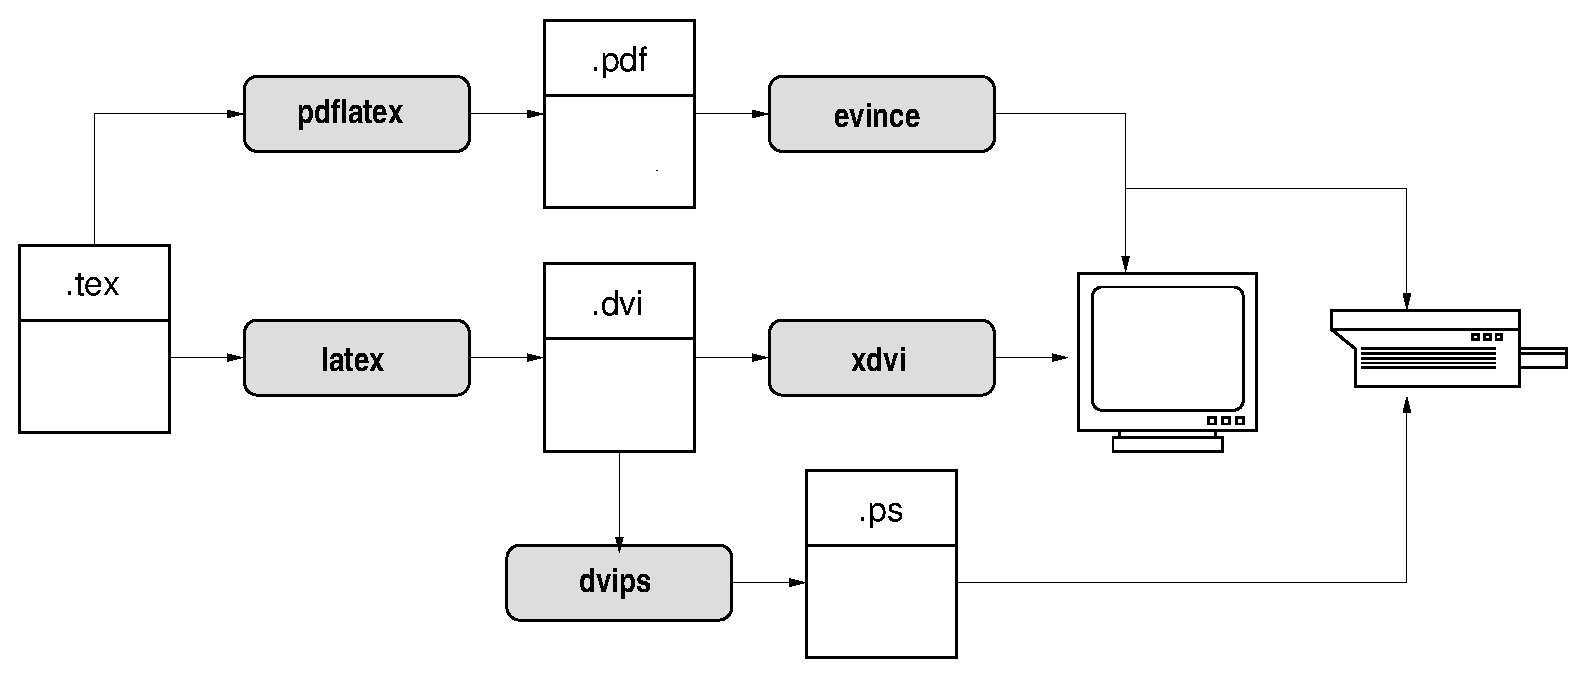
\includegraphics[width = 0.8\linewidth]{img/cycle.eps}
    \caption{UNIX中参与生成过程的工具}
    \label{fig:1.2}
\end{figure}

\subsection{显示}%visualisation有时翻译成可视化,有时翻译成显示,这个可以后期再统一一下。

在编译后,可以简单地使用\textsf{evince}程序来完成显示步骤。输入以下指令:

\dmh{evince \codereplace{文件名}.pdf \&}

这是一个\textsf{linux}下运行的十分直观的程序,能够给出一个方便阅读的文件预览。

\begin{exclamation}
    注意,不必在每次编译后都重新运行evince,它显示的内容会自动刷新。
\end{exclamation}

\subsection{打印}

对于\dm{pdf}格式,如何打印它这一问题就丢给了你的操作系统。关于这一点,没有特殊的注意事项。你有了一个文件,可以自由地处置它,无论是直接打印,还是根据你所处的环境来发挥才艺。

\begin{ii}
    从\dm{dvi}到\dm{ps}格式的转换需要调用dvips程序:

    \dmh{dvips \codereplace{文件名}.dvi}

    这可以生成一个PostScrpt格式的文件。这个格式也由Adobe创造,是一种打印机语言,可以看作\dm{pdf}的祖先。目前的打印机出厂即可识别这种打印机语言。我们可以说,文件发送到打印机时,十有八九传送的是PostScrpt格式的参数。对于PostScript格式的文件,有大量可以显示、修改这种文件的工具。
\end{ii}

\section{源文件的结构}

本节将介绍一种文档类型。实际上,所有\LaTeX 文档都具有相同的结构,形式如下:

\begin{dmd}
\backslash documentclass[\codereplace{类选项$_1$},\codereplace{类选项$_2$},...]\{\codereplace{类}\}\\
\backslash usepackage[\codereplace{包选项$_1$},\codereplace{包选项$_2$},...]\{\codereplace{包}\}\\
...\\
\codereplace{文前部分}\\
...\\
\backslash begin\{document\}\\
...\\
\codereplace{文本}\\
...\\
\backslash end\{document\}
\end{dmd}

如此一来,所有的\LaTeX 文档都可以按以下方式拆解。

\begin{itemize}
    \item 说明文档的\codereplace{类};
    \item 文前部分,包含以下内容:
        \begin{itemize}
            \item 使用特定的\codereplace{包};
            \item 多样的初始化和声明;
        \end{itemize}
    \item 文档主体,即我们将要亲手输入的全部内容,出现在\dm{\backslash begin\{document\}}和\dm{\backslash end\{document\}}之间。
\end{itemize}

以下介绍各部分的细节。

\subsection{文档的类}

所谓类,就是提供给\LaTeX 的一个指示,可以帮助\LaTeX 决定如何为文档的特定部分排版。根据具体使用的类不同,允许使用与否的指令可能不同(如\dm{\backslash chapter}在\dm{book}类中允许使用,在\dm{article}类中不允许使用)。另一方面,根据所选择的类,给出的命令会具有特定的含义(标题、材料表……)。在入门时\jz{
    实际上,我们可以在\dm{\backslash documentclass}前添加更多神奇的“咒语”……
},所有的\LaTeX 文档都必须以的指令开始——\dm{\backslash documentclass}接由花括号括住的类,包含以下几种:

\begin{itemize}
    \item \dm{article},用于文章;
    \item \dm{proc},用于电气与电子工程师协会(英:Institute of Electrical and Electronics Engineers,IEEE)会刊(英:proceeding)风格的文章;
    \item \dm{report},用于几十页篇幅的报告;
    \item \dm{book},用于图书或论文;
    \item \dm{letter},用于信件;
    \item \dm{slides},用于演示文档。
\end{itemize}

我们当然也可以为文档定义自己的类。类的配置项用方括号括住,可以是以下内容之一:

\begin{itemize}
    \item \dm{11pt, 12pt},用于全局地更改文字字号;
    \item \dm{twoside},用于生成适合双面打印的文档;
    \item \dm{draft},用于以草稿模式生成文档。
\end{itemize}

例如,输入:

\begin{dmd}
\verb|\documentclass{article}|
\end{dmd}

以上命令可以将全部配置项配置为默认值(字号为10 pt,单列,单面……)。

\begin{dmd}
    \backslash documentclass[12pt]\{article\}
\end{dmd}

以上命令将字号设置为12 pt(默认为10 pt)。再如:

\begin{dmd}
    \backslash documentclass[twoside, draft]\{report\}
\end{dmd}

以上命令可以以草稿模式生成适合双面打印的报告。

\subsection{文前部分}

文前部分是指位于子句\dm{\backslash documentclass}和子句\dm{\backslash begin\{documennt\}}间的区域。在这个区域中,我们可以明确想要包含的扩展(请看下一小节)%TODO
、初始化全局参数(如页边距等)、定义风格(如标题样式、序号等)、定义特殊的宏,等等。

\subsection{添加扩展}

\LaTeX 命令\dm{\backslash usepackage}可以与C语言的指令\dm{\#include}类比。这一命令允许添加\LaTeX 中满足宏或环境形式的功能\jz{
    相关内容将在下一章讲解。%TODO
}。目前,只需记住,我们可以在一行之内包含多个包:

\begin{dmd}
    \backslash usepackage\{\codereplace{包$_1$},\codereplace{包$_2$},\codereplace{包$_3$},...\}
\end{dmd}

如果\codereplace{包$_1$}、\codereplace{包$_2$}、\codereplace{包$_3$}拥有共同的配置项\codereplace{opt1},我们可以输入:

\begin{dmd}
    \backslash usepackage[\codereplace{opt1}]\{\codereplace{包$_1$},\codereplace{包$_2$},\codereplace{包$_3$}\}
\end{dmd}

相反,如果\codereplace{opt1}只涉及\codereplace{包$_2$},那么我们只能像这样写成两行:

\begin{dmd}
    \backslash usepackage\{\codereplace{包$_1$},\codereplace{包$_3$}\}\\
    \backslash usepackage[\codereplace{opt1}]\{\codereplace{包$_2$}\}
\end{dmd}

下面是两个例子:

\begin{dmd}
    \% 包graphicx带有配置项draft和xdvi\\
    \backslash usepackage[xdvi, draft]\{graphicx\}\\
    \% 包array和包subfig\\
    \backslash usepackage\{array, subfig\}
\end{dmd}

\begin{exclamation}
    根据定义,所有(类、包、命令的)的配置项参数都是\textit{可选的}。因此我们可以这样记:\LaTeX 中所有由方括号括住的参数\dm{[...]}都是非强制的。
\end{exclamation}

\section{开始!}

在本节,我们将尝试从一个只含几个排版命令的文档开始,介绍\LaTeX 的基本原理。

\begin{codelist}[1.1]{
    从你手中掉落的工具总是掉到最难够到的地方,或脆弱的物品上。\\
    这是\emph{墨菲}定律(loi de Murphy)的一个体现。
}  \begin{dmd}
    \verb+\documentclass{article}+\\
    \verb+\begin{document}+\\
    从你手中掉落的工具\\
    总是掉到最难够到的地方,\\
    或脆弱的物品上。\\
    ~\\
    \verb+这是\emph{墨菲}定律(loi de      Murphy)的+\\
    一个体现。\\
    \verb+\end{document}+
\end{dmd}
\end{codelist}

这个示例体现了\LaTeX 中的几个重要的原理,具体如下。

\paragraph*{空行代表跳转至下一段} \LaTeX 中的空行代表一段文字的结尾,因此在以上实例中,第一段从“\dm{从你}”开始,直到“\dm{物品上。}”结束。指令\dm{\backslash par}与空行等价,可以用来表示一段文字的起始。

\paragraph*{\LaTeX 会忽略换行}最终的文档中,换行并不由源文件中的换行决定。\LaTeX 会自动为各段文本\textit{打断、压缩、调节}文字,除非你有特殊的要求。

\paragraph*{\LaTeX 会忽略重复的空格}输入1个或18784个空格是等价的,比如源码中\dm{de}和\dm{Murphy}前插入的空格那样。此规则也适用于跳转段落:输入一行或多行空格是等价的。

\paragraph*{“\backslash ”是转义字符(caractère d’échappement;英:escape char)}“\backslash ”可以告诉\LaTeX 它后面的一系列字符是控制序列,也就是说,是最一般意义上的指令(或宏)。这里,它对“墨菲”一词生效,具体的效果由指令\dm{\backslash emph}控制。

\paragraph*{“\{”和“\}”}它们是\textit{组}的定界符,稍后会进一步解释它们。

\subsection{几个特殊字符}

就像符号“\backslash”的出现所暗示的那样,\LaTeX 中还有10个有特殊含义的符号,在此将其列出:

\begin{dmd}
    \verb+\ $ & % # ^ _ { } ~+
\end{dmd}

%todo 此前代码可以重新简化为verb

以下是一个使用部分特殊字符的案例:

\begin{codelist}[1.2]{
\textbf{是}下标:$x_{i+1}$,还是上标:$e^{i\pi}$;这是问题~1!
}\begin{verbatim}%毫无意义的段落
\textbf{是}下标:$x_{i+1}$,
还是上标:$e^{i\pi}$;
这是问题~1!%还是问题2?\end{verbatim}
\end{codelist}

目前,你需要知道:

\begin{itemize}
    \item \dm{\%}会使得\LaTeX 忽略当前行的剩余部分,因此,它是表示注释的符号(与C中的\dm{//}等价);
    \item \verb+~+代表不可拆分的空格\jz{
        见2.10节。
    },可以防止\LaTeX 在指定的位置断字。尽管有大量的情况需要插入这个符号来表示不可拆分(如所有形如“\verb+图~1+”的情况),然而,对于此类符号的使用,并没有系统化的规则。
    \item \dm{\$}用于标记公式的开始和结束。\LaTeX 遇到一个\dm{\$}符号时,它会切换到\celan{第3章}数学模式,直到遇到下一个\dm{\$}符号。
    \item \dm{\_}和\dm{\^{}}分别代表将文本转化为下标和上标。\textbf{注意},这两个符号只能在数学模式下使用。
    \item \dm{\{}和\dm{\}}分别表示组的开始和结束。本例中出现了两种组:一种出现在数学模式中,用于把将要放到下标或上标的“子公式”组合起来;另一种把将要设置成粗体的文字组合起来。
\end{itemize}

我们可以使用如下的指令来在让文档生成部分特殊字符:

\begin{dmd}
    \verb+\$ \& \% \# \{ \} \_+
\end{dmd}

这串指令可以输出“\$ \& \% \# \{ \} \_”。2.2.5小节%TODO
会解释如何使文档生成其余特殊字符(即\verb+\ ~ ^+)。

\subsection{调用指令}

你已经知道了,要想调用指令或宏,需要输入转义字符,并紧接着输入你想使用的宏名。%TODO 二对一
但是,\LaTeX 如何知道宏名的末尾在哪里呢?此处以用于生成\TeX 标识的\dm{\backslash TeX}为例来解释\yz{
    此例涉及对西文行文中空格的处理,不宜翻译。
}。

\begin{codelist}{
    \TeX book is for \TeX hackers.

    \TeX\  has some powerful macros.

    \LaTeX{} is a document preparation system
}\begin{verbatim}\TeX book is for \TeX hackers.

\TeX\  has some powerful macros.

\LaTeX{} is a document preparation system
    \end{verbatim}
\end{codelist}

\begin{exclamation}
    \verb*|\ |(其中\verb*| |代表空格)称作控制空格(espace de contrôle)。这个空格不会被\LaTeX 忽略。因此,指令“\verb*|et\ \ \ hop !|”会生成“et\ \ \ hop !”。实际上,以\dm{\backslash}\codereplace{函数}\dm{\{}\codereplace{参数}\dm{\}}的形式来调用宏是很好的习惯。因此,使用上例中的的第三种方式比第二种方式更佳。这种形式可以避免空格被忽略的情况发生\jz{
        所以他为什么要跟我们说这些?!
    }。因此,我们将使用\verb|the \teX{}book|来生成“the \TeX{}book”,使用“\verb*|\LaTeX{} is a ...|”来生成“\LaTeX{} is a ...”。
\end{exclamation}

\subsection{变音符号}

法国人往往对于使用\LaTeX 这件事忧心忡忡,因为法文中带有变音符号。别怕!你不必像表\ref{tab:1.1}\yz{
    该表与原书不完全相同。
}中展示的那样输入带有变音符号的字符。然而,你需要知道:无论是什么种类的字符,包括大写字母,我们都可以为其添加变音符号。

\begin{table}[H]
    \centering
    \begin{tabular}{|c|c|c|}
        \hline
        变音符号 & 源码 & 效果\\
        \hline
        尖音符 & \verb|\`z| & \`z \\
        钝音符 & \verb|\'z| & \'z \\
        长音符 & \verb|\^z| & \^z \\
        软音符 & \verb|\c{z}| & \c{z}\\
        分音符 & \verb|\"{z}| & \"{z}\\
        \hline
    \end{tabular}
    \caption{输入占7位(bit)的变音符号}
    \label{tab:1.1}
\end{table}

注意!虽然我们可以输入带有变音符号的字符,但不要忘记:这需要我们调用编码。目前,编码可能只针对地球上的某个地区。在法国,我们使用ISO 8859编码,配合拉丁文1区拓展。这套编码允许我们操纵美丽的变音符号。在详细阅读本书中专为使用法文书写文档的情况准备的章节\celan{第7章}之前,我们建议你在你源码的文前部分添加以下指令,以“攻克”法文文档的难关:

\begin{dmd}
    \begin{verbatim}
%源文件编码
\usepackage[latin1]{inputenc}
%TeX字体编码
\usepackage[T1]{fontenc}
%针对法文文档
\usepackage[francais]{babel}
    \end{verbatim}
\end{dmd}

\section{第一批工具}

以下几个宏和合字在文档中很常用,因此应当了解它们。首先,\LaTeX 会区分三种连接号:

\begin{itemize}
    \item \verb|-|,用于“Saint-Étienne”;
    \item \verb|--|,用于“page 12--24”;
    \item \verb|---|,在法文中用于插入语,如“une parenthèse --- comme cela”。
\end{itemize}

引号应以如下方式输入:

\begin{itemize}
    \item \verb|``|和\verb|''|可以输入英文中的引号\yz{
        此处与原书不同。原书前文输入变音符号时亦直接使用了单弯引号‘和’,但这两个符号作为命令参数时会导致编译错误,因此分别替换为反引号和直单引号。这可能是编译器的差异导致的。
    }——``English''。
    \item 如果键盘允许,对于法文,你可以输入«和»\jz{
        例如,在Linux系统下,分别按键盘的\fbox{Alt Gr}+\fbox{Z}和\fbox{Alt Gr}+\fbox{X}组合键(译注:适用于AZERTY键盘)。
    }。\textsf{babel}包的法文支持部分(参考第7章)%TODO
    允许我们通过\verb|\og|和\verb|fg|输入引号,由此,\verb|\og français\fg{}|这类命令是允许的—— «~français~»~。
\end{itemize}

以下是其余几个使用的命令:

\begin{itemize}
    \item \verb|\today|可以生成(编译时的)日期——2013年11月22日。
    \item \verb|\S|可以生成段落符号——\S。
    \item \verb|\ldots|可以在英文文档中生成省略号“\ldots”。但在法文文档中,应当输入三个点“...”(第7章会介绍更多有关法文排版的内容)。%TODO
\end{itemize}

最后要记得,英文中的双成分标点(ponctuation double;包括:;!?)前不加空格,但法文相反,它们的前面需要加空格。另外,在法国这个可爱的国家,我们几乎都靠右行驶。

\section{第一组报错}

\begin{ii}
    接下来,我们会看看\LaTeX 编译你的文档时闹的“情绪”。当我们放出编译指令时,我们会直接在终端看到这些输出。为了能让\LaTeX 得到充分使用,我们鼓励你在自己的环境下找到属于你自己的检查\LaTeX “\textsf{日志}”的方法。这些日体可以为你指明错误信息,以及编译过程中出现的其他警告。
\end{ii}

\subsection{症状}

如果你与\LaTeX 打交道,那么早晚有一天,你会看到屏幕上显示出类似这样粗旷的信息:

\begin{dmd}
    \linenumbers
    \begin{verbatim}
This is TeX, Version 3.1415 (C version 6.1)
(erreur.tex
LaTeX2e <1995/12/01>
(/usr/local/lib/texmf/tex/cls/article.cls
Document Class: article 1995/11/30 v1.3p Standard LaTeX document class
(/usr/local/lib/texmf/tex/clo/size10.clo)) (erreur.aux)
! Undefined control sequence.
l.5 paragraphe de ce \empha
                           {document}
?\end{verbatim}
\end{dmd}

几乎可以肯定,你看不懂这团内容。它是使用\LaTeX 处理文件\dm{erreur.tex}后终端上显示的内容。以下是文件全文\yz{
    文件正文意为:\dm{我觉得,在这样短的\backslash empha\{文档\}的第一段就有一个错误}。
}:

\begin{dmd}
    \begin{verbatim}
\documentclass{article}

\begin{document}
Il me semble bien qu’il y ait une erreur dans le
premier paragraphe de ce \empha{document} somme
toute assez court.
\end{document}
    \end{verbatim}
\end{dmd}

\subsection{诊断}

我们可以以一种简单的方式来解释以上错误信息。

\paragraph*{第1行}你使用的\TeX 版本为$\pi\pm 10^{-4}$。
\paragraph*{第2行}你想编译文件\dm{erreur.tex}。
\paragraph*{第3行}你使用了\LaTeXe ,版本日期为1995年12月。
\paragraph*{第4行~第5行}你使用了标准文档类\dm{article}。
\paragraph*{第6行}字号默认设置为10 pt。
\paragraph*{第7行}错误信息本身。
\paragraph*{第8行~第9行}\dm{erreur.tex}中造成错误的代码行和对应行号。
\paragraph*{第10行}\TeX 给出的短促且尤其让人焦虑的消息:\dm{?}。

第8行和第9行之间的“裂缝”精准地表明了\LaTeX 崩不住了的地方。以下消息:

\begin{dmd}
    ! Undefined control sequence.
\end{dmd}

向你说明了,\LaTeX 不认识你输入的指令。实际上,指令\verb|\empha|不存在。

\subsection*{治疗方案}

那么,当\LaTeX 给我们展示这个著名的“\dm{?}”时,我们应该怎么回答它呢?这里有3种最简短的方式,可以用来与\LaTeX 轻度交流。

\begin{itemize}
    \item 按回车键来忽略错误。
    \item 输入\dm{x}来退出编译。
    \item 输入\dm{r}让\LaTeX 继续编译,并忽略其他错误信息。
    \item 输入\dm{i}以插入一条更正信息并继续编译,但新插入的更正信息并不会出现在源文档中。
    \item 输入\dm{h}以获取更多关于该错误的信息。以下是本例中\TeX 提供给你的更多信息:\begin{verbatim}
Undefined control sequence :
  The control sequence at the end of the top line
  of your error message was never \def’ed. If you have
  misspelled it (e.g., ‘\hobx’), type ‘I’ and the
  correct spelling (e.g., ‘I\hbox’). Otherwise just
  continue, and I’ll forget about whatever was
  undefined.\end{verbatim}
\end{itemize}

\subsection{一些消息}

\TeX 和\LaTeX 会根据不同的情况给出大量错误消息,其中有一些在第一次面对时并不能读懂。然而,大多数经常出现的消息有以下类型:

\begin{itemize}
    \item \LaTeX 语法或保留字错误;
    \item 花括号没有成对出现;
    \item 在文本模式中出现了本应出现在数学模式中的内容;
    \item 数学模式没有关闭;
    \item 你忘记包含一个包;
    \item 编译过程无法结束;%TODO核实
    \item ……
\end{itemize}

\section{再说几句!}

现在,你知道了如何用\LaTeX 源码创建可打印的文件。同时,本章向你介绍了调用指令的原则。接下来,如果想要了解\LaTeX 语法中的不同功能,需要做的仅仅是去着手接下来的章节。%TODO
% \chapter{(占位)}
\chapter{需要了解的知识}

\begin{epigraphe}{《圣经·箴言》21:11}
    亵慢的人受刑罚,愚蒙的人就得智慧。\\智慧人受训诲,便得知识。
\end{epigraphe}


本章要研究使用\LaTeX 生成文档时的基本排版指令。我们将零散地处理用于突出显示、\LaTeX 标准环境、标题、页面下方的注释、页眉和页脚,以及浮动的环境。接下来,我们会介绍参考系统和\LaTeX 生成的辅助文件。最后,阅读到本章末尾的人将有机会读到一些关于断字的思考。

所有这些指令都将以其默认行为模式使用。也就是说,我们这里不介绍重新定义它们的方法。对应地,你将能够以传统的版式来生成文档。若要打出一篇更进阶的文章,你需要了解如何输入数学式(第3章)、一些关于科技文档的知识(第6章),以及包含图像的方法(第5章)。

\section{突出显示}

要了解\LaTeX 选用字体的机制,需要知道:我们通常通过4个参数来区别字体。

\begin{description}
  \item[族(famille)] 指字体的整体形状。默认情况下,\LaTeX 使用三种字体族:罗马体、\textsf{无衬线体}、\texttt{打字机体}。\LaTeX 中,以英文单词\emph{family}来指代字体族。
  \item[风格(style)] 指字体体现出的样式(英文以\emph{shape}指代),分为:\textit{意大利}、\textsl{倾斜}和小型大写字母风格(\textsc{petites capitales})\yz{
    本书翻译时,以楷体对应意大利风格、以仿宋体对应倾斜风格排版,按原文翻译。中文字体的族和风格往往是并列的,很少有交叉叠加的情况,因此在展示叠加效果时酌情保留原文。中文中很少见到类似小型大写字母的突出显示方式。因此,除了特意展示西文的部分外,本书忽略小型大写字母格式,必要时以其他风格取代。
  }。
  \item [字重(graisse)]指字体笔画的粗细(\LaTeX 中以\emph{serie}指代)。默认情况下有两种粗细:中等和\textbf{加粗}。
  \item [字号]字{\large 体}{\Large 的}{\LARGE 大}{\small 小}。
\end{description}


\subsection{族--风格--字重}

有两种不同的宏可以设置族、风格、字重这三个变量:\emph{指令}和\emph{声明}(如表\ref{tab:2.1}所示)。指令以花括号的形式将其参数括住。声明可以打断行文,同时修改三个变量之一,直到新的命令出现。总体上的规则是,我们使用指令来突出显示一个词或一组词:

\begin{table}
    \centering
    \begin{tabular}{|c|l|c|}
\hline
指令 & 声明 & 输出\\
\hline
\verb+\textrm{...}+ & \verb+{\rmfamily ...}+ & 罗马(roman) \\
\verb+\textsf{...}+ & \verb+{\sffamily ...}+ & \textsf{非衬线(sans sérif)} \\
\verb+\texttt{...}+ & \verb+{\ttfamily ...}+ & \texttt{打字机(machine à écrire)} \\
\hline
\verb+\textup{...}+ & \verb+{\upshape ...}+ & 正(droit) \\
\verb+\textit{...}+ & \verb+{\itshape ...}+ & \textit{意大利(italique)} \\
\verb+\textsl{...}+ & \verb+{\slshape ...}+ & \textsl{倾斜(penché)} \\
\verb+\textsc{...}+ & \verb+{\scshape ...}+ & 小型大写(\textsc{Petites Capitales}) \\
\hline
\verb+\textmd{...}+ & \verb+{\mdseries ...}+ & 中等(médium) \\
\verb+\textbf{...}+ & \verb+{\bfseries ...}+ & \textbf{加粗(gras)} \\
\hline
    \end{tabular}
    \caption{更改字体的声明}
    \label{tab:2.1}
\end{table}

\begin{codelist}[2.1]{
    \texttt{char}类型的\emph{变量}\textsl{总是}被编码为\textbf{8 位}。
}
\begin{verbatim}
\texttt{char}类型的\emph{变量}\textsl{总是}
被编码为\textbf{8 位}。\end{verbatim}
\end{codelist}

注意,在上面的命令中,指令\verb|\emph|(对应的声明是\verb|\em|,可以以更优雅的方式突出显示一组词)。相较声明,强烈建议使用\emph{指令}。当要修改文本的一部分时,使用指令是更明智的选择\jz{定义指令也是。}:

\begin{codelist}[2.2]{
    {\em \bfseries 马格马(Magma) \mdseries 的音乐就像一面镜子,每个人都能看到他自己的倒影。}
}
\begin{verbatim}
{\em \bfseries 马格马(Magma) \mdseries 的音乐
就像一面镜子,每个人都能看到他自己的倒影。}\end{verbatim}
\end{codelist}

接下来的例子展示了如何使用组。声明\verb|\slshape|出现在一个组中,因此它只在组内发挥作用。此外,组会继承它外层的组的参数。这样一来,“silence”一词会使用\textsf{非衬线}体(根据外层的组),并且\textsl{倾斜}展示(根据内层的声明):

\begin{codelist}[2.3]{
    \sffamily 在爵士乐中,{\slshape 沉默(silence)\/}永远是正确的。因此,这是一种充满万千可能的音乐。
}
\begin{verbatim}\sffamily 在爵士乐中,
{\slshape 沉默(silence)\/}永远是正确的。因此,
这是一种充满万千可能的音乐。\end{verbatim}
\end{codelist}

\subsection{意大利体校正}

另一个推荐使用指令而不是声明的理由是,与声明不同,指令可以实现\emph{意大利体校正}。所谓意大利体校正,是指在以意大利体显示的字符组后,有必要增加一个间距,使得这组字符不会“碰到”后面的词。这个间距与所涉及的字符有关\yz{此例展示不同情况下\emph{f}和a间距的细微差距,宜保留原文。例句意为:首长永远是对的。}:

\begin{codelist}[2.4]{
    le {\em chef} a toujours raison.\par
    le {\em chef\/} a toujours raison.\par
    le \emph{chef} a toujours raison.\par
}
\begin{verbatim}
le {\em chef} a toujours raison.\par
le {\em chef\/} a toujours raison.\par
le \emph{chef} a toujours raison.\par\end{verbatim}
\end{codelist}

我们可以看到,指令\verb|\emph|实现了校正,然而,若要使用声明,则需要明确地借助宏\verb|\/|来实现相同的效果。

\subsection{字号}

表\ref{tab:2.2}中展示的宏可以修改行文的字号。这些宏都是\emph{声明}。同时,对于每一个宏都存在同名的环境。

\begin{table}[ht]
    \centering
    \begin{tabular}{|c|c||l|c|}
\hline
\verb|\Huge| & {\Huge 宏大} & \verb|\normalsize| & {正常} \\
\verb|\huge| & {\huge 庞大} & \verb|\small| & {\small 小} \\
\verb|\LARGE| & {\LARGE 特大} & \verb|\footnotesize| & {\footnotesize 加小} \\
\verb|\Large| & {\Large 加大} & \verb|\scriptsize| & {\scriptsize 特小} \\
\verb|\large| & {\large 大} & \verb|\tiny| & {\tiny 微小} \\
\hline
    \end{tabular}
    \caption{修改字号}
    \label{tab:2.2}
\end{table}

\subsection{几个建议}

习惯上,我们应当尽量减少字体变化。实际上,如果字体变化得不合适宜或没有实际用处,尤其是喧宾夺主,影响了文档的可读性,看起来就会很低级。这里是有关使用字体变化的几条建议(仍然是习惯上的建议!):
\begin{itemize}
    \item 相较于使用其余指令,更多地使用\verb+\emph+(默认会将字体改为\emph{意大利}体)。
    \item 将\textbf{加粗}的机会留给特别重要的提示。
    \item 在法文文档中,几乎只在人名中使用小型大写字母(如Donald \textsc{Knuth})。
    \item \dm{打字机}字体族经常被用于生成编程语言的代码或类似的内容。
\end{itemize}

以下内容适用于能读懂其中道理的人……

除以上内容外,我们给出以下两个用于突出显示的情况,读者可以字形斟酌:改变字号、添加下划线(使用指令\verb|\underline|)。

\begin{origincitation}[克努特,\TeX Book{[9]}]
    也许那些希望{\tiny 小声说话}的诗人会让图书的字体频繁变化,但目前,只有一些字体狂人{\tiny (比如本手册的作者)}才喜欢这样做。
\end{origincitation}

\begin{origincitation}[迈克尔·古森斯(Michel Goossens)等,\\《\LaTeX 伴侣》(\emph{\LaTeX{} Companion}){[6]}]
    注意,出版行业认为,以添加下划线的形式来强调内容是不好的习惯。下划线只应用于一种情况——输出设备无法以其他方式突出显示内容,比如使用打字机。
\end{origincitation}

\section{环境}

\LaTeX 以\emph{环境}格式提供了一系列工具,具体结构是一个代码块,语法如下:

\begin{dmd}
    \verb+\begin+\codereplace{环境名}\verb|}|\\
    \verb|...|\\
    \verb+\end+\codereplace{环境名}\verb|}|\\
\end{dmd}

其中\codereplace{环境名}需要替换为具体的环境名称。我们目前遇到的第一个环境是\dm{document}。\verb|\begin| 和\verb|end|间的文字会以特殊版式展示。

\begin{exclamation}
    我们立刻注意到,环境中所有声明都是局部的。另外,当然可以在我们自己定义的环境中套用已经存在的环境。
\end{exclamation}

\subsection{居中和对齐}

想要居中显示几行文字,我们使用环境\dm{center}:

\begin{codelist}[2.5]{
    ……上一段的结尾。
    \begin{center}
        完美居中的\\
        几行文字\\
        且前后带有间距
    \end{center}
    然后继续下一段……
}
\begin{verbatim}
……上一段的结尾。
\begin{center}
  完美居中的\\
  几行文字\\
  且前后带有间距
\end{center}
然后继续下一段……\end{verbatim}
\end{codelist}

同样,我们可以轻易地借助环境\dm{flushright},让一个段落右对齐排列:

\begin{codelist}[2.6]{
    ……上一段的结尾。
    \begin{flushright}
      两行右对齐\\
      的文字
    \end{flushright}
    然后继续下一段……
    }
\begin{verbatim}
……上一段的结尾。
\begin{flushright}
  两行右对齐\\
  的文字
\end{flushright}
然后继续下一段……\end{verbatim}
\end{codelist}

注意,以上两个示例中,命令\verb|\\|起到了换行的功能。除一些特殊场景(表格、文档的标题和作者、特意的居中或对齐处理)外,不要使用这个命令——如果想要换行,需要使用空行或命令\verb|\par|。

\begin{flushleft}
    一般情况下,我们使用环境\dm{flushleft}时需要搭配命令\verb|\\|。但我们可以使用这个环境来生成右侧不对齐的文档,将换行的麻烦工作留给\LaTeX ,就像这段文字一样。(\textsl{译注}:此处给出本段原文。请注意右侧的换行的不对齐处理。En général, on emploie l'environnement \dm{flushleft} avec des commandes \verb|\\|. Mais on peut l'utiliser pour produire un paragraphe comme celui-ci, non justifié à droite, en laissant à \LaTeX{} le soin d’insérer les sauts de lignes.)
\end{flushleft}

%TODO 排查代码下正文内容
\begin{exclamation}
    绝大部分环境都会重启一行来插入内容。然而,重要的是:环境只是在插入内容的位置\emph{中断}当前段落,而不是结束当前段落。你可以在前两个实例中看到,“然后继续下一段……”这句话前没有缩进。另外,\LaTeX 贴心地在每个环境前后都留了一段空白。
\end{exclamation}

我们可以注意到,前面的三个环境分别代表以下三个声明:

\begin{itemize}
    \item \verb|\centering|;
    \item \verb|\raggedleft|;
    \item \verb|\raggedright|。
\end{itemize}

例如,我们可以这样写\yz{
    实际上,Emacs代表Editor MACroS。本例是对Emacs的调侃。
}:

\begin{codelist}[2.7]{
    Emacs代表:

    {\centering Emacs\\Makes\\
      A\\Computer\\Slow\\}
}
\begin{verbatim}
Emacs代表:

{\centering Emacs\\Makes\\
  A\\Computer\\Slow\\}\end{verbatim}
\end{codelist}

\subsection{列表}

\LaTeX 提供了三种呈现\emph{列表}的基本环境:\dm{itemize}、\dm{enumerate}、\dm{description}。如果它们都不能满足你,也可以定义属于你自己的\celan{9.5节}列表。但目前,先来看看标准的列表。

首先,\dm{itemize}可以生成不编号的项目列表。在法文版本中,一级列表会使用连接号(---)标记;在其他版本中,会使用点($\bullet$)标记:

\begin{codelist}[2.8]{
……一句话的结尾。
\begin{itemize}
\item 在复杂的计算中,分子的系数需要传递给分母;
\item 不应当写逗号。
\end{itemize}
然后行文继续。
}
\begin{verbatim}
……一句话的结尾。
\begin{itemize}
\item 在复杂的计算中,
  分子的系数需要
  传递给分母;
\item 不应当写逗号。
\end{itemize}
然后行文继续。\end{verbatim}
\end{codelist}

环境\dm{enumerate}遵循类似的规则,只不过项目会被编号。一个环境中可以套用另一个环境。下面的例子中,我们同时展示了\dm{ enumerate}和\dm{description}环境:

\begin{codelist}[2.9]{
    ……还是一句话的结尾。
    \begin{description}
    \item[\TeX] \TeX{}book;
    \item[\LaTeX] 两本重要的书:
      \begin{enumerate}
      \item 《\LaTeX{}:一个文档准备系统》(\emph{\LaTeX{}: A Document Preparation System})。
      \item 《\LaTeX{}伴侣》。
      \end{enumerate}
    \end{description}
    跟之前一样,接下来段落继续……
}
\begin{verbatim}
……还是一句话的结尾。
\begin{description}
\item[\TeX] \TeX{}book;
\item[\LaTeX] 两本重要的书:
  \begin{enumerate}
  \item 《\LaTeX{}:一个文档
    准备系统》(\emph{\LaTeX{}: 
    A Document Preparation System})。
  \item 《\LaTeX{}伴侣》。
  \end{enumerate}
\end{description}
跟之前一样,接下来段落继续……\end{verbatim}
\end{codelist}

至于环境\dm{description}的列表,在我们习惯的文档处理中没有对应内容。不幸的是,对于\LaTeX 初学者,它最好的结果是被误用,最差的结果是被无视。

\subsection{制表}

环境\dm{tabbing}可以用于打字机上使用的那种老式制表过程%TODO查证
。我们可以使用指令\verb|\=|来放置定位标记,并使用指令\verb|\>|来在定位标记之间移动。此外,\verb|\\|可以用来换行。

\begin{codelist}[2.10]{
  \begin{tabbing}
    左倾 \= 中间立场 \= 右倾 \\
    \> 中立派 \\
    \> \> 保守派 \\
    xxxxxxxxx \= \kill
    \> 无观点
    \end{tabbing}
}
\begin{verbatim}
\begin{tabbing}
  左倾 \= 中间立场 \= 右倾 \\
  \> 中立派 \\
  \> \> 保守派 \\
  字字字字字 \= \kill
  \> 无观点
\end{tabbing}\end{verbatim}
\end{codelist}

我们可以从这个例子中看到两个规则:

\begin{itemize}
    \item 可以在制表时插入一行“模板”,并且使用指令\verb|\kill|来隐藏这一行;
    \item 如果已经存在定位标记,新的指令\verb|\=|可以在逻辑上移除它们。
\end{itemize}

\subsection{表格}

\LaTeX 中用于生成\emph{表格}的环境称为\dm{tabular}。表线的处理可能不太精细,但对于线条简单的表格,结果可以接受\jz{
    附录B提供了一些提示,可以用来找到能够生成更复杂表格的包。
}:

\begin{codelist}[2.11]{
    嚯:
    \begin{tabular}{|r|c|}
        \hline
        俩 & 仨 \\
        五个 & 六个  \\ \hline
      \end{tabular}
}
\begin{verbatim}
嚯:
\begin{tabular}{|r|c|}
  \hline
  俩 & 仨 \\
  五个 & 六个  \\ \hline
\end{tabular}\end{verbatim}
\end{codelist}

通过这个例子,我们可以得到以下结论。

\begin{itemize}
    \item 环境\dm{tabular}会等待输入一个参数,应用指示表格的格式。每列都应该以一个定位字符表示。
    \begin{itemize}
        \item \dm{r}:右对齐。
        \item \dm{c}:居中。
        \item \dm{l}:左对齐。
    \end{itemize}
    \item 字符\verb|&|用于分隔不同列。
    \item 指令\verb|\\|用于跳转至下一行。
    \item 布局字符串中的\dm{|}表示插入纵向表线。
    \item 横向表线由指令\verb|\hline|插入。
\end{itemize}

因此,我们可以自由地调整\verb|\hline|和\dm{|}的数量,以隐藏或显示表线。包\textsf{array}可以满足一些关于表格的幻想。

\begin{exclamation}
大多数环境都会另起一行,但\dm{tabular}不会。\dm{tabular}会紧接当前的文本生成\linebreak 表格。
\end{exclamation}

此外,我们还可以使用参数来精确地指定表格竖直方向上的位置:

\begin{codelist}[2.12]{
一个表:\begin{tabular}[b]{|c|} 
甲\\乙
\end{tabular}
,另一个表:\begin{tabular}[t]{|c|} 
丙\\丁\end{tabular}
}
\begin{verbatim}
一个表:\begin{tabular}[b]{|c|} 
  甲\\乙
\end{tabular}
,另一个表:\begin{tabular}[t]{|c|} 
  丙\\丁
\end{tabular}\end{verbatim}
\end{codelist}

我们可以看出,参数\dm{b}将表格“放置”在当前行上,参数\dm{t}将表格“悬挂”在当前行下。如果没有参数,表格会在竖直方向上居中,就像前面的例子一样。

显然,表格可以不插入句子中,而可以单独成段,比如配合环境\dm{center}被单独居中。

\subsection{模拟终端}

环境\dm{verbatim}可以将其内容逐字插入文档。因此,无论什么字符,甚至是特殊字符,都可以使用它来插入,如插入一个\textsf{C++}代码片段:

\begin{codelist}[2.13]{\ttfamily
  \begin{tabbing}
    cl\=ass pixel \{\\
      \>int x, y;\\
    public:\\
      \>pixel(int i=0, int j=0);\};
  \end{tabbing}
}
\ttfamily
\backslash begin\{verbatim\}
\begin{verbatim}
class pixel{
  int x,y;
public:
  pixel(int i=0, int j=0);};\end{verbatim}
\backslash end\{verbatim\}
\end{codelist}

\begin{exclamation}
我们可以在环境\dm{verbatim}中写任何内容,\emph{除了}以下字符串——\verb|\end{verbatim}|!\\
\end{exclamation}

有两个指令可以像\dm{verbatim}一样生成文本片段:\verb|\verb|和\verb|\verb*|。带有星号的版本可以将空格“\verb| |”显示为“\verb*| |”的形式。

这两个指令的参数不使用花括号括起,而夹在任何一种可以满足以下两个条件的符号之间:不能是特殊符号、不能在参数中包含:

\begin{codelist}[2.14]{
  使用{\ttfamily \#include<stdlib.h>}可以
  包含C语言标准库的原型。
}
\begin{verbatim}
使用\verb+#include<stdlib.h>+可以
包含C语言标准库的原型。\end{verbatim}
\end{codelist}

\begin{exclamation}
在任何情况下,指令\verb|\verb|都不能出现在其他指令的参数中,无论这个指令是\linebreak 什么。
\end{exclamation}

\subsection{引用语}

环境\dm{quote}和\dm{quotation}可以在文本中引用内容。首先来看\dm{quote}:

\begin{codelist}[2.15]{
  ……仍然是一句话的结尾。
\begin{quote}
  万物相关。\hfill\textbf{爱因斯坦}

  有件事情是不确定的,
  那就是所有事情都是确定的。
  \hfill\textbf{帕斯卡}
\end{quote}
然后继续被打断的段落……
}
\begin{verbatim}
……仍然是一句话的结尾。
\begin{quote}
  万物相关。\hfill\textbf{爱因斯坦}

  有件事情是不确定的,
  那就是所有事情都是确定的。
  \hfill\textbf{帕斯卡}
\end{quote}
然后继续被打断的段落……\end{verbatim}
\end{codelist}

指令\verb|\hfill|可以插入一段在水平空间上\celan{\S 4.2.4}无限延伸的空白。环境\dm{quotation}有一些细微的差别:

\begin{codelist}[2.16]{
  ……仍然是一句话的结尾。
\begin{quotation}
  人有许多缺陷,但我们若能
  想到他们被创造的那个年代,
  就能对此感到宽容。\par
  \raggedleft 阿方斯·阿莱
  (Alphonse Allais)
\end{quotation}
然后继续被打断的段落……
}
\begin{verbatim}
……仍然是一句话的结尾。
\begin{quotation}
  人有许多缺陷,但我们若能
  想到他们被创造的那个年代,
  就能对此感到宽容。\par
  \raggedleft 阿方斯·阿莱
  (Alphonse Allais)
\end{quotation}
然后继续被打断的段落……\end{verbatim}
\end{codelist}

实际上,对于这两个环境,根据莱斯利·兰波特的介绍,一个(\dm{quote})是为引用一条或多条短的内容而准备的,另一个(\dm{quotation})是为引用一条长的内容而准备。

\section{页边注}

指令\verb|\marginpar|可以在页边缘创建一个小段落,语法如下:

\begin{dmd}
\backslash marginpar\{\codereplace{文字}\}
\end{dmd}

对于双面打印的模式,为了区分左侧和右侧的页面,我们可以使用如下指令\yz{
  原书有误。此处已更正。
}:

\begin{dmd}
\backslash marginpar[\codereplace{左侧文字}]\{\codereplace{右侧文字}\}
\end{dmd}

其中\codereplace{左侧文字}和\codereplace{右侧文字}会根据当前页码的奇偶性在页面左侧或右侧呈现。如此一来,以下指令:

\begin{dmd}
\backslash marginpar[这!]\{嚯!\}
\end{dmd}\marginpar[这!]{嚯!}

会生成你在本页页边缘看到的内容。

\section{标题}

表\ref{tab:2.3}给出了\LaTeX 种可用的\emph{章节}命令。对于类型为\dm{article}的文档,指令\verb|\chapter|不可用;对于类型为\dm{letter}的文档,任何标题类型都不可用。目前,你需要了解以下两点:

\begin{itemize}
  \item 使用指令生成的每个标题都可以自动\emph{编号},并可以在必要时列入目录。
  \item 使用指令\verb|\tableofcontents|可以生成目录,并将其插入该指令所在的位置。
\end{itemize}

\begin{table}[ht]
  \centering
  \begin{tabular}{|l|l|l|}
    \hline
    \verb|\part{...}| & \verb|\chapter{...}| & \\
    \verb|\section{...}| & \verb|\subsection{...}| & \verb|\subsubsection{...}| \\
    \verb|\paragraph{...}| & \verb|\subparagraph{...}| &  \\
    \hline
  \end{tabular}
  \caption{章节指令}
  \label{tab:2.3}
\end{table}

\begin{ii}
此外,所有的标题指令都带有可以自定义的相关类型。% TODO
总的来说,这些指令会自动生成标题前后的间距。如此一来,指令前后的任何空行都会被忽略。
\end{ii}

\begin{codelist}[2.17]{
  ……一句话的结尾。
  \section*{3.2\quad 结论}
  最终,……
}
\begin{verbatim}
……一句话的结尾。
\section{结论}
最终,……\end{verbatim}
\end{codelist}

每种标题指令都带有一种“带星”形式(例如,\verb|\section*|),可以插入不参与编号的标题。但需要注意,这种标题不会出现在\celan{\S 2.9.2}目录中。与节(section)相关的标题指令中可以接受参数,用于明确目录中展示的内容。例如:

\begin{dmd}
\verb+\section[张三]{太帅了!}+
\end{dmd}

可以在文档中插入节标题“太帅了!”,但在目录中将其展示为“张三”。

\section{页面底部的注释}

有一种方便的方式可以在页面底部插入注释:使用指令\verb|\footnote{|\codereplace{文本}\verb|}|。注释会自动编号,且在默认情况下按章重新编号。如下是\LaTeX 可以实现的效果:

\begin{codelist}[2.18]{
  无论如何,指令\texttt{footnote}$^a$可以在页面底部插入注释。\\
  ————\\%TODO 
  {\footnotesize $^a$正如其名。}
}
\begin{verbatim}
无论如何,指令\verb+footnote+
\footnote{正如其名。}可以在页面
底部插入注释。\end{verbatim}
\end{codelist}

在一些特殊情况中,\verb|\footnote|不能生成我们想要的效果。此时,有必要分两步走:

\begin{enumerate}
  \item 使用指令\verb|\footnotemark|放置\emph{注释标记};
  \item 当条件允许时,使用指令\verb|\footnotetext|在页面底部输入\emph{文字}。
\end{enumerate}

例如,在表格中插入注释似乎有点棘手,此时可以这样写:

\begin{codelist}[2.19]{
  \begin{tabular}{cc}
    甲 & 乙$^a$ \\
    丙 & 丁\\
  \end{tabular}\\
  ————\\
  {\footnotesize $^a$一个注释。}
}
\begin{verbatim}
\begin{tabular}{cc}
  甲 & 乙\footnotemark \\
  丙 & 丁
\end{tabular}\footnotetext{一个注释。}\end{verbatim}
\end{codelist}

\section{页眉和页脚}

\LaTeX 生成页眉和页脚的标准指令有些简陋,但这里也值得一提,因为这些指令对于一些特定情况已经足够了。

\begin{ii}
关于这些指令,在这里就不讲更多内容了,因为\dm{fancyhdr.dvi}中介绍的fancyhdr包易用得多,也提供了比\LaTeX 的标准指令多得多的有趣选项。本书关于使用此包生成页眉页脚的详细解释在10.4节。
\end{ii}

如果不调用其他包,可以在文档的文前部分使用指令\verb|\pagestyle|来指定页眉页脚的风格:

\begin{dmd}
\verb|\pagestyle{|\codereplace{风格}\verb|}|
\end{dmd}

其中,参数\codereplace{风格}可以从以下值中选择:

\begin{itemize}
  \item \dm{empty},不显示页眉和页脚;
  \item \dm{plain},默认风格,页脚居中显示当前页码;
  \item \dm{headings},在页眉显示一定的内容,根据文档风格的不同而不同(例如,在双面的\dm{report}文档中,会显示当前的章名或节名);
  \item \dm{myheadings},自定义插入内容。
\end{itemize}

此外,使用指令\verb|\thispagestyle|,可以变更或指定当前页的风格。

\section{浮动环境}

\LaTeX 为其优秀的用户提供了使用\emph{浮动}环境的可能性。这种环境的特点是,其内容会被“漂浮地”渲染到正文中。也就是说,\LaTeX 通过一种算法,综合考虑一系列参数,在文档中为这种环境挑选位置。

\begin{exclamation}
\LaTeX 中的环境\dm{figure}和\dm{table}并不仅仅可以用来插入图片和表格,这一点与它们的名字相反。实际上,这两种环境只是将其内容浮动起来,并且为添加图题或表题提供了可能性。实际上,这两种环境中可以是你喜欢的任何内容,也不一定要是图形。
\end{exclamation}

\subsection{图(figure)和表(table)}

环境\dm{figure}一般用来插入图像,而环境\dm{tale}一般用于插入表格。这两种环境都可以带有自己的小标题,使用语法如下:

\begin{codelist}[2.20]{
  此段包含了浮动环境“figure”,
其内容可以在页面中浮动。
% \begin{figure} 插环境会报错
  \begin{center}
三\\
O丁O\\
四\\
Figure 1: 有个老丁头
  \end{center}
%   \caption*{有个老丁头}
% \end{figure}

}
\begin{verbatim}
此段包含了浮动环境“figure”,
其内容可以在页面中浮动。
\begin{figure}
  \begin{center}
    三\\
    O丁O\\
    四\\
  \end{center}
  \caption{有个老丁头}
\end{figure}\end{verbatim}
\end{codelist}

注意到,使用指令\verb|\caption|可以生成图题或表题。文本“Figure 1:”会自动生成,并给出对应该图片的编号。这种“风格”也是可以自定义的。

\subsection{确定位置}

我们可以在\verb|\begin|后面用方括号中给出参数,来让\LaTeX 尝试依此放置浮动的内容,具体如下:

\begin{itemize}
  \item \dm{h},放置在源码中出现的原位置;
  \item \dm{t},放置在页面顶部;
  \item \dm{b},放置在页面底部;
  \item \dm{p},放置在单独的页面上。
\end{itemize}

注意,有时我们会为如何放置浮动环境而抓狂。为了不因此而烦躁,需要理解(并接受)下面这一点:\LaTeX 会综合考虑多个参数来安排环境\dm{figure}和\dm{table}的位置,其中包括:

\begin{itemize}
  \item 放置在页面顶部和底部的浮动环境的最大数量;
  \item 顶部和底部放置有浮动环境的页面占全部页面的最大可接受比例;
  \item 浮动环境前后的空白。
\end{itemize}

如果你在放置图片时遇到了关于其位置的问题\jz{并且你确定它真的成问题……},我们建议你遵循以下建议:

\begin{itemize}
  \item 如果你尝试写“\textsl{如下图所示:}”之类的话,并且希望紧接着放一个图片,\emph{不要使用环境}\dm{figure}!。
  \item 尽量使用\emph{参考}系统,例如写成“如图3所示”。
  \item 我们总是喜欢放一些超大图片——缩小它们!
  \item 如果你的表格太长,把它放到附录中去。无论如何,它会让读者很难受。
  \item \LaTeX 中的参数经过精心研究,目的是平衡文档中文字和图片的数量。所以如果你的文档是连环画,请做好最坏的准备……
  \item 只有到了\textbf{印刷你的最终版文档}时才有必要去纠结图片的位置。
\end{itemize}

\subsection{图片列表}

使用指令\verb|\listoffigures|(对应地,\verb|\listoftables|)可以在文档中插入全部图片(对应地,表格)的列表。列表会出现在指令所在的位置。此类指令会生成扩展名为\dm{.lof}(对应地,\dm{.lot})的文件。此外,与插入节标题时使用参数指定目录中展示的内容类似,指令\verb|\caption|中也可以带有一个参数,来控制其在列表中显示的内容。默认情况下,列表中会显示图题(对应地,表题):

\begin{dmd}
\verb|\caption[嚯]{|你可以在这里尽情写些人生故事,因为无论你写多长,它都不会出现在图片列表中,因为我们已经指定了这个无比长的小标题显示成“嚯”……\verb|}|
\end{dmd}

\section{引用}

\LaTeX 的引用系统以为对象编号的方式允许你以符号的方式操作文档中任何部分的序号,因此,没有必要去记忆一个图片究竟是图4还是图5。\LaTeX 通过这种方式为你减少了很多工作,并且这种方式可以通过几行文字就能解释清楚。

\subsection{原理}

为了在文档中成功使用引用,我们需要做两件事:第一,在文档中添加符号标记;第二,调用这个标记来进行引用,要么引用相应对象的序号,要么引用其出现的页码。这样简单的方式简化了工作:

\begin{enumerate}
  \item 使用指令\verb|\label|来添加标记:\\
  \verb|\label{|\codereplace{标记内容}\verb|}|\\
  其中\codereplace{标记内容}是一个不带有特殊字符的字符串;
  \item 使用指令\verb|\ref|来引用相应对象的序号:\\
  \verb|\ref{|\codereplace{标记内容}\verb|}|
\end{enumerate}

使用\verb|\pageref|,可以引用相应页码:

\verb|\pageref{|\codereplace{标记内容}\verb|}|

\subsection{需要引用什么?}

我们可以引用的内容如下:

\begin{itemize}
  \item 各级标题;
  \item 浮动环境(\dm{figure}、\dm{table}……);
  \item 数学式(参见第3章);
  \item 带编号列表(如\dm{enumerate})的项;
  \item 等等。
\end{itemize}

如下的示例综合了三种引用指令:

\begin{codelist}[2.21]{
  \section*{3.5\quad 二次方程}
二次方程即以下形式的方程 :
\begin{equation}
  ax^2 + bx + c = 0 \tag{2.12}
\end{equation}
第13页3.5节中的方程2.12这么说完那么说……
}
\begin{verbatim}
\section{二次方程}\label{sec-2dg}
二次方程具有以下形式 :
\begin{equation}
  ax^2 + bx + c = 0 \label{equ}
\end{equation}
第\pageref{sec-2dg}页\ref{sec-2dg}节
中的方程\ref{equ}这么说完那么说……\end{verbatim}
\end{codelist}

在这个示例中,我们引用了对象\verb|\section|和另一个\verb|\equation|。此外,我们还引用了这个关于方程的节所在页的页码。

\begin{exclamation}
当在浮动环境中放置\verb|\label|时,请一定将其放置指令\verb|\caption|的\textbf{后面}。否则,引用会“指向”当前的节,而不是图形。
\end{exclamation}

\section{辅助文件}

为了进一步理解引用的机制,我们需要检查以下\LaTeX 编译源文件时向你的硬盘中写入了什么。目前,你可以看到的文件有如下格式。

\begin{description}
  \item[\fbox{\texttt{dvi}}] 文档中的图片。
  \item[\fbox{\texttt{log}}] \LaTeX 在最近一次编译时的“自言自语”。一般情况下,它多多少少代表了你编译时在终端上看到的内容。
  \item[\fbox{\texttt{aux}}] 辅助文件,储存引用、页码、标题等信息。
  \item[\fbox{\texttt{toc}}] 目录文件。
  \item[\fbox{\texttt{lof}}] 图片列表文件。
\end{description}

\subsection{与引用的交互}

\LaTeX 以如下的方式处理引用:在第一次编译时,在文件\codereplace{文件名}\dm{.aux}中储存引用,其中\codereplace{文件名}是你的文档的文件名。我们可以在如下示例中看到其解决引用的问题时的机制和原理,在该示例中,我们尝试引用位于第35页的第3节中的一个名为\dm{truc}的标记\yz{“truc”意为“小东西”。}。

\begin{enumerate}
  \item 在第一次编译时,\LaTeX 在\dm{.aux}格式的辅助文件中存储该标记的号码(在本例中,存储其所在节的序号)和该标记出现页的页码(如图\ref{fig:ref1}所示)。
  
  \begin{figure}[ht]
    \begin{center}
      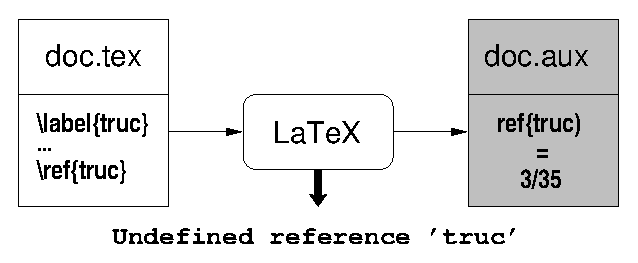
\includegraphics{img/ref1.eps}
    \end{center}
    \caption{使用\dm{.aux}的第一次编译}
    \label{fig:ref1}
  \end{figure}

  因此,此次编译时,会\LaTeX 发送警告,指出标记\dm{truc}未定义。
  \item 我们会进行第二次编译,这次编译会使用辅助文件的内容(如图\ref{fig:ref2}所示)。
  
  \begin{figure}[ht]
    \begin{center}
      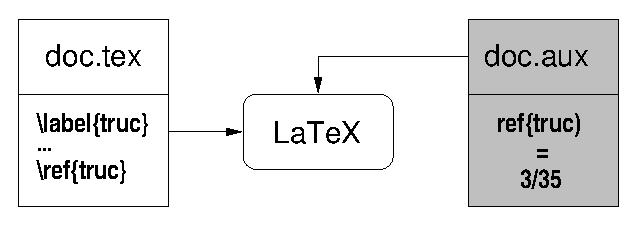
\includegraphics{img/ref2.eps}
    \end{center}
    \caption{使用\dm{.aux}的第二次编译}
    \label{fig:ref2}
  \end{figure}
\end{enumerate}

在以下情况中的引用定义是不正确的。

\begin{enumerate}
  \item 你插入了一个新的标记,并且在插入标记后第一次编译(引用\emph{未被定义})。此时,对于新插入的标记,会得到如下形式的消息:
  
  \begin{dmd}
  Reference 'vlunch' on page 2 undefined on input line 17.
  \end{dmd}

  \item 你在文档中引入的变化无疑会改变页码或对象(图片、方程等)的位置,因此引用会被\emph{错误定义}。在编译结束时,你会看到如下警告:
  
  \begin{dmd}
  Label(s) may have changed.\\
  Rerun to get cross-references right.
  \end{dmd}

  \item 你引用了一个不存在的标记。在这种情况下,再编译八百次也无济于事。
\end{enumerate}

\subsection{与目录的交互}

对于目录,你会发现,其原理与引用是类似的。在文档中插入指令\verb|\tableofcontents|意味着目录将会分两步创建,具体如下。

\begin{enumerate}
  \item 第一轮遍历会收集文档中与\emph{表题}相关的信息,并将其存入文件\codereplace{文件名}\dm{.toc}中(如图\ref{fig:toc1}所示)。
  
  \begin{figure}[ht]
    \begin{center}
      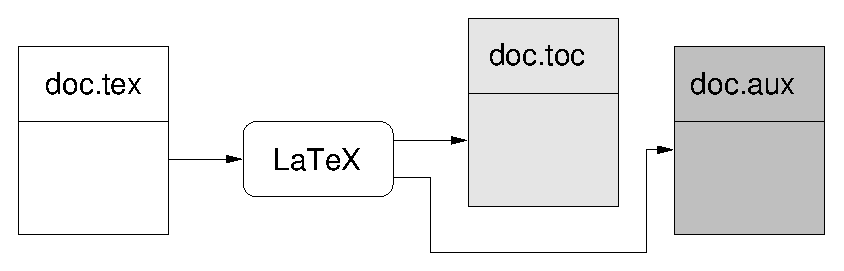
\includegraphics{img/toc1.eps}
    \end{center}
    \caption{使用\dm{.toc}的第一次编译}
    \label{fig:toc1}
  \end{figure}

  \item 第二轮遍历会使最终的文档中包含\codereplace{文件名}\dm{.toc},因此,目录也会被包含(如图\ref{fig:toc2}所示)。
  
  \begin{figure}[ht]
    \begin{center}
      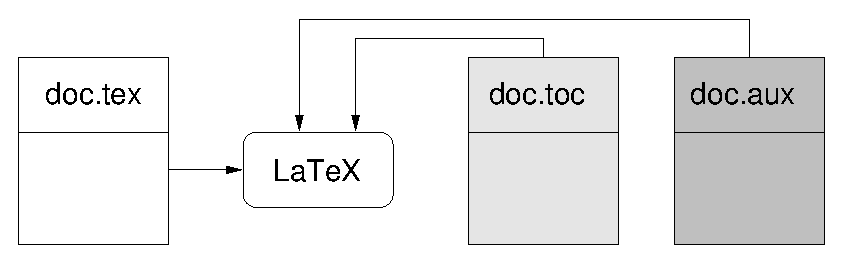
\includegraphics{img/toc2.eps}
    \end{center}
    \caption{使用\dm{.toc}的第二次编译}
    \label{fig:toc2}
  \end{figure}

\end{enumerate}

你可能会遇到这种情况:在写草稿时,文档已经包含了目录指令(\verb|tableofcontents|),而你又添加了新的章节指令。在这种情况下,新的章节只有经过\textbf{两次}编译后才会显示在目录中。

\subsection{一些建议}

要养成为每个文档生成目录的习惯。实际上,\LaTeX 会围绕你的\dm{.tex}文件生成多个文件\jz{
  这还没有涉及参考文献、索引、术语目录等。
}。另外,在起草文档时,不必过于关心目录是否时刻更新——它早晚会更新的!实际上,只有在\textbf{印刷}之前才有必要去确认所有的引用都是正确的。

最后,就像我们在不再能确定目标文件时会时不时运行一下\dm{make clean}指令一样,在看起来一切都运行不正常时,删掉辅助文件\celan{\S B.2}并重新编译是个好习惯。

\section{断字的处理}

\LaTeX 依靠\TeX 对特定的语言来实现不同的断字效果。这种算法在\TeX Book的附录H中有描述,也体现出\TeX 最成功的一面。通过检查文档打断段落的方式,可以识别出文档是不是由\LaTeX 生成的,因为其他很多软件都喜欢以在单词间添加更多空间的方式来处理此类问题。然而,也会有一些\LaTeX 无法正确断字的情况。在这种情况下,\LaTeX 会以以下两种“吓人的”信息之一为你给出警告:

\begin{dmd}
Underfull \backslash hbox (badness 1810) detected at line 33
\end{dmd}

或

\begin{dmd}
Overfull \backslash hbox (14.24376pt too wide) detected at line 41
\end{dmd}

\TeX 在很底层用你的文档生成一系列\emph{字盒}。每个字符都装入合适的字盒,字盒组合成词,再以类似的方式组合成行、成段,然后成页面。

这里以一种简单的方式总结和介绍原理。我们可以简单地理解为,\TeX 在水平模式下操纵\verb|\hbox|来组合单词,在竖直模式下操纵\verb|\vbox|来生成页面。此外,组合这些字盒时,\TeX 如果觉得结果不太美观,就会用以上述两种信息警告你。信息的含义如下。

\begin{itemize}
  \item \verb|Underfull \hbox|表示字盒组合得有些稀疏。通过显示badness的值,\TeX 会告诉你它认为当前行“有多丑”。如果一行文字排列得很完美,该值为0。在最差的情况下,该值为10000.
  \item \verb|Overfull \hbox|表示字盒有些太挤了。\TeX 可以以\dm{pt}为单位显示文字越界深入边缘的长度。
\end{itemize}

如果一个页面过于稀疏,\LaTeX 会以\verb|\vbox|代替\verb|\hbox|显示类似的消息。表\ref{tab:2.4}展示了同一句话的不同疏密程度\yz{
  表中的例句出自法国古典主义戏剧大师高乃依(Pierre Corneille)的戏剧《熙德》(\textit{Le Cid}),意为“哦,愤怒!哦,绝望!哦,宿敌!”。
}排列效果。

\newcommand{\phrase}[1]{\noindent\makebox[\width +
#1][s]{%
  Ô rage ! ô désespoir ! ô vieillesse ennemie !}\par}
\begin{table}[ht] 
\begin{center}
  % \addtolength{\extrarowheight}{4pt} 
  \begin{tabular}{|l|c|}
    \hline
    效果 & 评价 \\
    \hline
    % \typeout{UNDERFULL HBOX AUTORISE}%
    \phrase{1.0cm}  & 稀疏\\
    \phrase{0.75cm} & 稀疏\\
    \phrase{0.45cm} & 稀疏\\
    \hline
    % \typeout{UNDERFULL HBOX AUTORISE}%
    \phrase{0cm}    & 理想 \\ 
    \hline
    \phrase{-0.1cm} & 过密\\
    \phrase{-0.2cm} & 过密\\
    \phrase{-0.25cm} & 过密\\
    \hline
  \end{tabular}
  \caption{横向的不同疏密排列}
  \label{tab:2.4}
\end{center} 
\end{table}

\begin{ii}
  \makebox[\width+2pt][s]{可以在文档选项中启用\dm{draft},来使在出现\dm{Overfull \backslash hbox}问题的位置的侧栏显示一个黑色的\char"258C}
  方块,就像本段的侧栏一样。这个选项可以帮助快速定位导致问题的行。
\end{ii}

\subsection{控制断字}

对于以下情况,\LaTeX 的断字处理可能遇到困难。

\begin{itemize}
  \item 它不能识别需要打断的词——这是个极端情况。
  \item 不能打断的对象占据了需要打断的位置,例如\verb+\verb|...|+或方程类型的对象。
\end{itemize}

这里提供以下几个控制断字的方法。

\begin{exclamation}
如果以下方法都不能使你满意(如果你的句子中包含太多\TeX 不能打断的对象,就会产生这种情况),就只能想办法更换表达方式来规避问题了。
\end{exclamation}

\subsubsection{引导断字}

我们可以通过在必要的位置插入指令\verb|\-|来指出可以断字的位置,从而帮助\LaTeX 实现断字。例如,如果\LaTeX 不能成功地打断“nonmaiçavapamieu”\yz{
  作者的生造词,形似句子“Non, mais ça ne va pas mieux.”,意为“不,没有变得更好”。
}一词,我们可以输入:

\begin{dmd}
\verb|non\-mai\-ça\-va\-pa\-mieu|
\end{dmd}

如果这个词频繁出现,为了避免反复像上面这样给出指示,可以在文前部分输入指令\linebreak \verb|\hyphenation|:

\begin{dmd}
\verb|\hyphenation{non-mai-ça-va-pa-mieu}|
\end{dmd}

这样就可以告诉\LaTeX 这个生词的断字方式。

\subsubsection{强制断字}

通过输入指令\verb|\linebreak[|\codereplace{数字}\verb|]|,我们可以强制断字,但这样做可能带来灾难性的后果——如果你明白我的意思。参数\codereplace{数字}可以调节指令\verb|\linebreak|。你可以“腼腆”地给出指示——\verb|\linebreak[0]|,或是给出不容置疑的命令——\verb|\linebreak[4]|。

指令\verb|\pagebreak[|\codereplace{数字}\verb|]|可以打断页面。另一方面,还有两个指令可以用来换页:

\begin{itemize}
  \item \verb|\clearpage| 完成当前页面,换页另起。
  \item \verb|\cleardoublepage| 完成当前页面,并在双面模式下从奇数页另起。
\end{itemize}

这两条指令会强制\LaTeX 在布局过程中插入所有浮动的图像。%TODO 所以这句是在说啥???

\begin{ii}
另外一种对某些情况很实用的手动介入方式是将当前页面纵向长度加长,需要调用如下指令:

\begin{dmd}
  \backslash enlargethispage
\end{dmd}

指令需要给出尺寸,且其后需要插入一个空行:

\begin{tabbing}
  \verb|\enlargethispage{10cm}   | \= \leftarrow 针对过短的页面 \\
  ~\\
  \verb|[……一段过长的文字……]|\\
  \verb|\clearpage| \> \leftarrow 明确延长10 cm的页面的结尾
\end{tabbing}
\end{ii}

\subsubsection{防止断字}

有三种方式可以强制\LaTeX 不打断文本。

\begin{enumerate}
  \item 通过\verb|~|插入不可打断的空格。
  \item 通过\verb|\mbox{|\codereplace{单词}\verb|}|将词放入一个字盒中\jz{
    这是因为\TeX \textbf{永远不会}打断字盒。
  }。
  \item 对于防止换行使用指令\verb|\nolinebreak|:
  
  \begin{dmd}
  \backslash nolinebreak[\codereplace{数字}]
  \end{dmd}

  同样,为了防止换页,可以使用如下指令:

  \begin{dmd}
    \backslash nopagebreak[\codereplace{数字}]
  \end{dmd}

  其中\codereplace{数字}与\verb|\linebreak|或\verb|\pagebreak|中的作用一致。

\end{enumerate}

\section{小结}

本章介绍了\LaTeX 的标准功能。你如果专心地阅读至此,应该已经可以创建任何类型的简单文档了(目前还不能处理带有公式和图表的文档)。即使你还不能自由地定制你的文档,你的文档的排版质量也会足够好,不需要你提出很多形而上学的问题,如多大的页边距才“理想”、标题和文字间留出多少空白才“合适”……实际上,\LaTeX 中的默认特性已经足够满足全世界范围内有关印刷的大部分实用性规则。


\chapter{数学排版}

这十二使徒的名:头一个叫西门,又称彼得……——《圣经·马太福音》10:2

毫无疑问,\LaTeX 最实用和有趣\jz{
    没错,没错!真的有人排公式纯是为了玩!
}的特性就是可以生成数学公式。它生成的公式自然、美观,并且不需要你做任何工作\jz{
    或者只需要你去做两三件小事情。
}。另外,如果你有使用关于某个特定的公式编辑器点来点去的糟糕记忆,现在就偷着乐吧:现在,编写公式不需要鼠标了!使用\LaTeX 生成公式是一个广大的领域,我们这里仅仅会介绍一些用于生成“常用”公式所需的基本知识。因此,本章仅仅包含操作\LaTeX 公式的简短介绍。

\begin{ii}
\LaTeX 的标准指令足以生成大多数常见的数学方程。然而,建议使用美国数学学会(英:American Mathematical Society)发布的扩展amsmath和amssymb。可以在很多情况下,这两个扩展可以简化格式化过程。
\end{ii}

\section{编写数学公式的两种方式}

\LaTeX 可以识别两种数学公式。第一种是在文本中直接插入公式,就像这样:$ax+b=c$;另一种是将若干公式写在环境中,例如:
$$
{\rm d} U = \delta \mathcal{W} +\delta \mathcal{Q} 
$$

这两种模式都遵循一系列原则,涉及不同符号的字号和位置。如下示例使用了两种模式:

\begin{codelist}[3.1]{
  函数$f(x)$定义如下:
\begin{displaymath}
  f(x)=\sqrt{\frac{x-1}{x+1}}
\end{displaymath}
若其导函数存在,求其导函数。
}\begin{verbatim}
函数$f(x)$定义如下:
\begin{displaymath}
  f(x)=\sqrt{\frac{x-1}{x+1}}
\end{displaymath}
若其导函数存在,求其导函数。
\end{verbatim}
\end{codelist}

这个示例告诉我们,我们可以使用\dm{\$}符号来进入“内部”数学模式,并再次使用\dm{\$}符号退出。此外,这里使用了环境\dm{displaymath},这是最简单的生成数学式的方法。使用\verb|\[|和\verb|\]|也可以达成后者的效果(参见3.7.1节。)

3.7节会介绍\LaTeX 的不同环境。

\section{常用指令}

\subsection{上标和下标}

正如1.4.1小节提到的,指令\verb|_|和\verb|^|分别可以生成\emph{下标}和\emph{上标}。若需要这两条指令处理多个字符,需要将这些参数“打包”到一组花括号中。

\begin{center}
  \begin{tabular}{lc|lc|lc}
    \verb|x_2| & $x_2$ & \verb|x_{2y}| & $x_{2y}$ & \verb|x_{t_0}| & $x_{t_0}$ \\
    \hline
    \verb|x^2| & $x^2$ & \verb|x^{2y}| & $x^{2y}$ & \verb|x_{t^0}| & $x_{t^0}$ \\
    \hline
    & &  \verb|x^{2y}_{t_0}| & $x^{2y}_{t_0}$ & \verb|x_{t^1}^{2y}| & $x_{t^1}^{2y}$
  \end{tabular}
\end{center}

\subsection{分式和根式}

生成\emph{分式}和\emph{根式}的指令如下:

\begin{itemize}
  \item 指令\verb|\frac{|\codereplace{分子}\verb|}{|\codereplace{分母}\verb|}|可以生成分式,\codereplace{分子}会排在分数线上方,\codereplace{分母}会排在分数线下方;
  \item 指令\verb|\sqrt[|\codereplace{n}\verb|]{|\codereplace{arg}\verb|}|可以生成分式,表示变量\codereplace{arg}的\codereplace{n}次方根。
\end{itemize}

注意,这两种指令在字间模式和方程模式下生成的效果不同。对于分式$\frac{1}{\sin x + 1}$和根式$\sqrt{3x^2-1}$,他们在方程模式下的显示效果为:
\begin{displaymath}
  \frac{1}{\sin x + 1}\quad \sqrt{3x^2-1}
\end{displaymath}

作为介绍这两条指令的结尾,我们来看看它们是如何套用的:

\begin{codelist}[3.2]{
  \begin{displaymath}
    \sqrt{\frac{1+\sqrt[3]{3x+1}}
              {3x+\frac{1-x}{1+x}}}
  \end{displaymath}
}\begin{verbatim}
\begin{displaymath}
  \sqrt{\frac{1+\sqrt[3]{3x+1}}
             {3x+\frac{1-x}{1+x}}}
\end{displaymath}
\end{verbatim}
\end{codelist}

\subsection{符号}

\subsubsection{常用符号}

表\ref{tab:3.1}展示了部分生成你可能需要的符号的宏。

\begin{table}[hbt]
  \centering
  \begin{tabular}{cccccccc}
    \verb+\pm+       & $\pm$  & \verb+\otimes+      &  $\otimes$ & 
    \verb+\cong+     & $\cong$  & \verb+\imath+     &  $\imath$     \\
    \verb+\mp+       & $\mp$  & \verb+\oslash+      &  $\oslash$ &  
    \verb+\subset+   & $\subset$  & \verb+\jmath+   &  $\jmath$     \\
    \verb+\div+      & $\div$  & \verb+\odot+       &  $\odot$     & 
    \verb+\supset+   & $\supset$  & \verb+\ell+     &  $\ell$         \\
    \verb+\ast+      & $\ast$  & \verb+\leq+        &  $\leq$       & 
    \verb+\subseteq+ & $\subseteq$  & \verb+\aleph+ &  $\aleph$     \\
    \verb+\times+    & $\times$  & \verb+\geq+      &  $\geq$       & 
    \verb+\supseteq+ & $\supseteq$  & \verb+\nabla+ &  $\nabla$     \\
    \verb+\bullets+  & $\bullet$  & \verb+\equiv+   &  $\equiv$   & 
    \verb+\in+       & $\in$      & \verb+\|+       &  $\|$         \\
    \verb+\circ+     & $\circ$  & \verb+\ll+        &  $\ll$         & 
    \verb+\ni+       & $\ni$    & \verb+\partial+   &  $\partial$  \\
    \verb+\star+     & $\star$  & \verb+\gg+     &  $\gg$         & 
    \verb+\emptyset+ & $\emptyset$  & \verb+\wedge+ &  $\wedge$     \\
    \verb+\setminus+ & \backslash & \verb+\sim+ &  $\sim$       & %setminus与unicode-math包冲突,会显示空白
    \verb+\forall+   & $\forall$  & \verb+\vee+   &  $\vee$         \\
    \verb+\oplus+    & $\oplus$  & \verb+\simeq+    &  $\simeq$   & 
    \verb+\infty+    & $\infty$  & \verb+\cup+    &  $\cup$         \\
    \verb+\ominus+   & $\ominus$  & \verb+\approx+   &  $\approx$ & 
    \verb+\exists+   & $\exists$  & \verb+\cap+   &  $\cap$   
  \end{tabular}
  \caption{常用数学符号}
  \label{tab:3.1}
\end{table}

\begin{ii}
我们盘点了latexsym和amssymb包中的近450个符号(参见附录C)%TODO
。目的不是介绍它们!表\ref{tab:3.1}是标准符号中的一部分,我们认为它们可能是最常用的那一批——除了完全偶然出现的$\aleph$\yz{
  aleph,希伯来文字母表的第一个字母。
}。也许这证明了作者的数学水平不太高。
\end{ii}

\subsubsection{省略号}

为了节省篇幅,数学式中经常使用省略号。省略号有三种,指令\verb|\dots|可以生成点“放置在”基线上的省略号:

\begin{codelist}[3.3]{
$C=\{\vec{c}_0,\vec{c}_1,\dots,
    \vec{c}_N\}$
为$N$个颜色的集合。
}\begin{verbatim}
$C=\{\vec{c}_0,\vec{c}_1,\dots,
    \vec{c}_N\}$
为$N$个颜色的集合。
\end{verbatim}
\end{codelist}

指令\verb|\cdots|生成的省略号圆点上下居中,就像等号一样:

\begin{codelist}[3.4]{
  $\vec{\mu}=\frac{1}{N}
(\vec{c}_0+\vec{c}_1+\cdots+\vec{c}_N)$
为$N$个颜色的平均值。
}\begin{verbatim}
$\vec{\mu}=\frac{1}{N}
(\vec{c}_0+\vec{c}_1+\cdots+\vec{c}_N)$
为$N$个颜色的平均值。
\end{verbatim}
\end{codelist}

最后,指令\verb|\vdots|和\verb|\ddots|主要在矩阵中使用(参见3.6节、例3.15)。这两个指令分别可以生成$\vdots$和$\ddots$这两种省略号。

\subsubsection{箭头}

用于生成箭头的指令可以使用以下简单的方法来记忆:

\begin{itemize}
  \item 所有指令均以\dm{arrow}结尾;
  \item 必须带有前缀\dm{left}或\dm{right},表示方向;
  \item 可以带有前缀\dm{long},表示加长;
  \item 指令的第一个字母可以改为大写,表示箭头使用双线;
  \item 可以连写\dm{left}和\dm{right},表示双向箭头。
\end{itemize}

综上:

\begin{center}
  \begin{tabular}{lll|lll}
    \verb+\rightarrow+ & 表示  &$\rightarrow$ &
    \verb+\Longleftarrow+ & 表示 & $\Longleftarrow$ \\
    \verb+\Leftarrow+ & 表示 &$\Leftarrow$ &
    \verb+\Longleftrightarrow+ & 表示 &$\Longleftrightarrow$
  \end{tabular}
\end{center}

\subsubsection{希腊字母}

可以以一种极简单的方式使用希腊字母:打出它们的名字。也就是说,\verb|\alpha|表示$\alpha $,\verb|\pi|表示$\pi $。将指令的第一个字母改为大写,表示将对应希腊字母改为大写:\verb|\Gamma|表示$\Gamma $。注意,不是所有大写希腊字母都有对应的指令,如果要将$\alpha $改为大写,直接使用字母A即可(指令\verb|\Alpha|不存在)。

\subsubsection{实数集}

科技文档的作者常常会面临一个“至关重要”的问题:“我们应当如何打出代表实数集的字母`R'?”关于这个问题,这里分享几个观点。从历史上看,似乎最初的数学资料上将实数符号排版为加粗的形式(“令$x \in \mathbf{R}$”),老师们会使用粉笔反复在字母“R”上描几遍,来代表这个符号。这种比较烦琐的方法促成了我们“更熟悉”的写法:“令$x \in \mathbbm{R}$”。因此,出现了不同的流派:$\mathbf{R}$、ℝ,等等。如果你想自己选择,那么有如下包和指令供你选择:

\begin{itemize}
  \item \textsf{bbm}提供的指令\verb|\mathbbm{R}|可以生成$\mathbbm{R}$、指令\verb|\mathbbmss{R}|可以生成$\mathbbmss{R}$,等等;
  \item \textsf{bbold}提供的指令\verb|\mathbbm{R}|可以生成$\mathbbm{R}$;
  \item \textsf{amssymb}提供的指令\verb|\mathbb{R}|可以生成ℝ、指令\verb|\mathbf{R}|可以生成$\mathbf{R}$。
\end{itemize}

\section{函数}

\subsection{标准函数}

要生成经典的数学函数(如对数函数、三角函数等),需要使用\LaTeX 预装的函数来实现,这里是一个示例:

\begin{codelist}[3.5]{
$\sin^2x + \cos^2 x=1$
}\begin{verbatim}
$\sin^2x + \cos^2 x=1$
\end{verbatim}
\end{codelist}

如果不使用\LaTeX 函数:

\begin{codelist}[3.6]{
$sin^2x + cos^2x=1$
}\begin{verbatim}
$sin^2x + cos^2x=1$
\end{verbatim}
\end{codelist}

二者的区别在于,\LaTeX 会将字符串\dm{cos}视为一系列变量(因此生成意大利体),而将函数\verb|\cos|生成为罗马体的“cos”。另一个区别是对可能存在的下标的处理(参见以下\verb|\max|的示例)。以下函数都是\LaTeX 的标准数学函数。

\begin{itemize}
  \item 各种三角函数:\verb|\sin|、\verb|\cos|、\verb|\tan|。在前面加\dm{arc},可以得到对应的反函数。在后面加\dm{h},可以得到双曲三角函数。
  \item 自然对数和常用对数\yz{
    指以10为底的对数,标准的写法为$\lg$。本书以原书习惯为准,约定使用$\log$。
  }分别使用函数\verb|\ln|和\verb|\log|。
  \item 函数\verb|\sup|、\verb|\inf|、\verb|\max|、\verb|\min|、\verb|\arg|可以用于如下形式的数学式中:
  
  \begin{codelist}[3.7]{
    \begin{displaymath}
      T=\arg \max_{t<0} f(t)
    \end{displaymath}
  }\begin{verbatim}
\begin{displaymath}
  T=\arg \max_{t<0} f(t)
\end{displaymath}
  \end{verbatim}
  \end{codelist}
\end{itemize}

注意搭配\verb|\max|使用下标操作符\dm{\_}的结果。

\subsection{积分、求和和其他极限}

\LaTeX 使用一套简单的语法来生成\emph{积分}、\emph{求和}等内容,具体如下:

\begin{dmd}
\backslash \codereplace{操作}\verb|_{|\codereplace{下界}\verb|}^{|\codereplace{上界}\verb|}|
\end{dmd}

其中\codereplace{操作}可以是\dm{sum}、\dm{prod}、\dm{int}、\dm{lim}之一,\codereplace{上界}和\codereplace{下界}会排列在操作符号的周围。例如:

\begin{codelist}[3.8]{
  对此等比数列求和:
\begin{displaymath}
  \sum_{i=0}^{n}q^i=
  \frac{\quad 1-q^{n+1}}{1-q}
\end{displaymath}
}\begin{verbatim}
  对此等比数列求和:
\begin{displaymath}
  \sum_{i=0}^{n}q^i=
  \frac{1-q^{n+1}}{1-q}
\end{displaymath}
\end{verbatim}
\end{codelist}

类似地,使用指令\verb|\prod|可以生成求积符号$\prod$。
以下是使用积分的示例:

\begin{codelist}[3.9]{
对于$x>0$,定义自然对数如下:
\begin{displaymath}
  \ln(x)=\int_{1}^{x}\frac{1}{t}
  \,\mathrm{dt}
\end{displaymath}
}\begin{verbatim}
对于$x>0$,定义自然对数如下:
\begin{displaymath}
  \ln(x)=\int_{1}^{x}\frac{1}{t}
  \,\mathrm{dt}
\end{displaymath}
\end{verbatim}
\end{codelist}

指令\verb|\,|可以在“dt”前插入很小的空格(参见3.5.1小节)。你如果更喜欢\emph{线积分},可以使用\verb|\oint|,这个指令可以生成符号$\oint$。好了,这里会给出一个关于极限的示例,相信你可以看懂:

\begin{codelist}[3.10]{
  $f(x)$在$x_0$处存在极限$\ell$:
\begin{displaymath}
  \lim_{x\rightarrow x_0}f(x)=\ell
\end{displaymath}
}\begin{verbatim}
$f(x)$在$x_0$处存在极限$\ell$:
\begin{displaymath}
  \lim_{x\rightarrow x_0}f(x)=\ell
\end{displaymath}
\end{verbatim}
\end{codelist}

希望你能注意到示例中漂亮的$\ell$。为了巩固一下关于两种数学模式的知识,这里给出相同的数学式,但它们这次会镶嵌在行文中:求和,$\sum_{i=0}^{n}q^i=\frac{1-q^{n+1}}{1-q}$;求积分,$\ln(x)=\int_{1}^{x}\frac{1}{t}\,\mathrm{dt}$;求极限,$\lim_{x\rightarrow x_0}f(x)=\ell$。

\section{重叠的符号}

\subsection{操作符\dm{not}}

操作符\verb|\not|可以生成特定关系的“否定”样式:

\begin{codelist}[3.11]{
  令实数$x \not\in I$……
}\begin{verbatim}
  令实数$x \not\in I$……
\end{verbatim}
\end{codelist}

\verb|\not|的输出结果就是在其下一个符号上加上一道“斜杠”。\textbf{注意},这个操作符并不能总是呈现出完美的效果,例如\verb|$\not\longrightarrow$|会显示为$\not\longrightarrow$。但对于宽度合适的符号,它给出的结果还能令人满意。

\subsection{“变音符号”}

对于特殊的数学概念,经常需要\jz{
  实际上,一些名副其实的大数学家很喜欢这种符号上面的小帽子。一些人甚至还喜欢在上面叠两层、三层……
}在符号上加“变音”符号。以下是可用的符号示例:

\begin{center}
  \begin{tabular}{lc@{\quad}lc@{\quad}lc}
    \verb+\hat{x}+  &$\hat{x}$  & \verb+\check{x}+&$\check{x}$&
    \verb+\breve{x}+&$\breve{x}$\\
    \verb+\acute{x}+&$\acute{x}$& \verb+\grave{x}+&$\grave{x}$&
    \verb+\tilde{x}+&$\tilde{x}$\\ 
    \verb+\bar{x}+  &$\bar{x}$  & \verb+\dot{x}+&$\dot{x}$&
    \verb+\ddot{x}+ &$\ddot{x}$\\  
  \end{tabular}
\end{center}


\subsection{向量}

有两种\jz{
由埃迪·索德雷(Eddie Saudrais)开发的包\textsf{esvect}可以为向量生成更好看的箭头。
}方式可以得到向量:

\begin{itemize}
  \item 对于小些的符号,可以使用\verb|\vec|,因为这个指令是用于添加“变音”符号的。
  \item 对于其他情况,可以使用\verb|\overrightarrow|。
\end{itemize}

\begin{codelist}[3.12]{
设$\overrightarrow{A\!B}$在基底
$(\vec{\imath},\vec{\jmath})$
下定义。
}\begin{verbatim}
设$\overrightarrow{A\!B}$在基底
$(\vec{\imath},\vec{\jmath})$
下定义。
\end{verbatim}
\end{codelist}

注意,\verb|$\vec{A\!B}$|会显示为$\vec{A\!B}$(关于\verb|\!|的用途,参见3.5.1小节)。此外,指令\verb|\imath|和\verb|\jmath|分别可以生成不带点的字母i和j:$\imath$、$\jmath$。

\subsection{指令\dm{stackrel}}

指令\verb|\stackrel|可以将两个符号叠放在一起:

\begin{dmd}
\verb|\stackrel{|\codereplace{符号$_1$}\}\{\codereplace{符号$_2$}\}
\end{dmd}

\codereplace{符号$_1$}会置于\codereplace{符号$_2$}上方。例如:

\begin{dmd}
\verb|x\stackrel{f}{\longmapsto}y|
\end{dmd}

以上代码会生成$x\stackrel{f}{\longmapsto}y$。

\section{两个重要原则}

为了掌握\LaTeX 生成数学式的方法,需要知道以下两个原则。

\begin{description}
  \item[空格] \LaTeX 会忽略数学式中夹带的空格,因此\verb|$x+1$|和\verb|$x + 1$|生成的结果是相同的。\LaTeX 会在它认为最合适的地方添加空格。
  \item[文本] 任何的符号组都会被当作同一系列变量或函数对待,因此\verb|$x=t avec t>0$|\yz{
    此问题几乎只在西文排版中出现,因此保留原文。avec可理解为“且其中”。
  }会生成“$x=t avec t>0$”,而不是你所期待的“$x=t$ avec $t>0$”
  \jz{
    数学式中夹带文本的问题只会在使用\dm{displaymath}系列的环境时显现出来。毕竟,使用“\dm{\$x=t\$ avec \$t>0\$}”总是可以的!
  }。
\end{description}

在了解了两个原则后,来看看入门如何处理相关的问题。

\subsection{数学模式的空格}

首先需要知道,\LaTeX 选择添加空格的方式一般是正确的。然而,如果有一天你非要去\rlap{ㄨㄨㄨㄨ}吹毛求疵,表\ref{tab:3.2}可以帮助你在数学式中插入空格。在该表格中,我们在两个$\Box$符号之间夹入不同的空格指令,来展示它们的效果。

\begin{table}[ht]
  \begin{center}
    \begin{tabular}{|ll|ll|ll|ll|}
      \hline
      \verb+\!+ & $\Box\!\Box$ &
      \emph{无指令} & $\Box\Box$ &
      \verb+\,+ & $\Box\,\Box$ &
      \verb+\:+ & $\Box\:\Box$ \\
      \hline
      \verb+\;+ & $\Box\;\Box$ &
      \verb*+\ + & $\Box\ \Box$ &
      \verb|\quad| & $\Box\quad\Box$ &
      \verb|\qquad| & $\Box\qquad\Box$ \\
      \hline
    \end{tabular}
    \caption{数学模式中的空格}
    \label{tab:3.2}
  \end{center}
\end{table}

对于那些关注“毛”“疵”的人,要强调一下,本书在等比数列的示例(参见3.3.2小节)中偷偷了在分子上添加了一些空格,以让分式中的两个$q$稍微对齐。如果按照默认的生成方式,结果会是这样的:

\begin{displaymath}
  \sum_{i=0}^{n}q^i=
  \frac{1-q^{n+1}}{1-q}
\end{displaymath}

不知道这个关于$q$的故事是否为你带来了更敏锐的观察力。

\subsection{数学模式中的文本}

在数学式中插入文本,最简单的方法是将文本“装箱”,并适当地插入空格:

\begin{codelist}[3.13]{
设数列$(u_n),(v_n)$:
\begin{displaymath}
  u_n=\ln n\quad
  \mbox{且}\quad v_n=(1+\frac{1}{n})^n
  \label{ex-maths-suite}
\end{displaymath}
}\begin{verbatim}
设数列$(u_n),(v_n)$:
\begin{displaymath}
  u_n=\ln n\quad
  \mbox{且}\quad v_n=(1+\frac{1}{n})^n
  \label{ex-maths-suite}
\end{displaymath}
\end{verbatim}
\end{codelist}

你可以在4.4.1小节找到关于指令\verb|\mbox|的细节。如果你已经在考虑使用包\textsf{amsmath},相比于使用\verb|\mbox|,也可以考虑使用指令\verb|\text|。

\section{阵列(array):简单且高效}

阵列环境\dm{array}可以满足生成大多数数学式的需求。正如其名,它可以将对象排列成一行行、一列列的样子。实际上,它和环境\dm{tabular}对应。也正如\dm{tabular}一样,\dm{array}也不会换行。


\chapter{成为小魔仙}
\chapter{图像}

\begin{quote}
    不可为自己雕刻偶像,也不可作什么形像……不可跪拜那些像,也不可事奉它。
    
    \hfill《圣经·申命记》5:8
\end{quote}

今天,在文档中插入画、照片或其他类型的图像看起来稀松平常,这是由于印刷技术的性能日渐强大、运行日渐稳定。但我们需要在20世纪80年代,也就是\TeX 仍在发展的背景下去看问题。在那个年代,打印机刚刚出现,个体无法接触到具有高质量打印能力的设备。然而,很多打印的解决方案将会诞生,其中的大部分都会基于PostScript语言,因为使用PostScript已经成为了\emph{事实上的}标准做法。

围绕\LaTeX ,有很多在文档中插入图像的解决方案。我们会注意到,其中的一些使用了\textsf{metafont}(管理\LaTeX 字体的实用工具),一些编写了环境\dm{picture},还有一些使用了PIC\TeX 的代码。此处不会介绍这些解决方案,因为我们认为它们有些难以上手。即便如此,你还是需要知道这些解决方案的存在。本书采纳的操作图像的方式是:在\LaTeX 源码中插入封装了相关内容的PostScript格式文件。这种文件可以使用\textsf{xfig}、\textsf{gnuplot}、\textsf{gimp}等绘图软件生成。

\section{开胃小菜}

了解一下用于画线的指令\verb|\rule|多少有些用处:

\begin{dmd}
\backslash rule[\codereplace{纵向位置}]\{\codereplace{长度}\}\{\codereplace{宽度}\}
\end{dmd}

其中\codereplace{纵向位置}可以根据需要在竖直方向上平移线,另外两个参数足以描述线的形态:

\begin{codelist}[5.1]{
    这些都是“线”:
\begin{center}
    \rule[1ex]{1mm}{5mm}
    \quad\rule{1in}{0.4pt}
    \quad\rule[-0.5em]{1em}{1em}
\end{center}
}\begin{verbatim}
这些都是“线”:
\begin{center}
    \rule[1ex]{1mm}{5mm}
    \quad\rule{1in}{0.4pt}
    \quad\rule[-0.5em]{1em}{1em}
\end{center}
\end{verbatim}
\end{codelist}

\section{图像文件的格式}

为了在文档中包含图像,需要插入\emph{文件}。\LaTeX 的配置允许其夹带PS(即PostScript)和EPS(即Encapsuled PostScript)类型的文件,至于要插入的文件是由什么软件生成的,\LaTeX 并不关心。你如果认为PostScript格式有诸多限制,那么需要认识到以下事实。

\begin{itemize}
    \item 所有\emph{合格}的“矢量”绘图软件都具有将图表导出为EPS格式文件的功能。对于印刷设备,这种格式已经成为标准。
    \item 所有图片都可以转换为EPS格式。在UNIX系统中,可以借助程序\textsf{convert}完成这一操作\jz{
        如果你的系统中没有这个程序,请查找“ImageMagick”套件来获取它。
    }。我们也可以使用软件\textsf{gimp}(一款自由软件,可以用于修图和创建数字图片)完成这一操作,它也适用于其他操作系统。
\end{itemize}

\section{包\textsf{graphicx}}

\LaTeX ,或者说\TeX ,在最初的设想中并不以操作图像(图片、图画等)为目的。基于此,大量扩展被提出,但它们都不是必需的,也不能真正独立于操作系统。

\subsection{标准}

目前,\LaTeX 设计师似乎同意将\emph{图像的}扩展统一起来。1994年年末,两个扩展走入了人们的视野:

\begin{itemize}
    \item \textsf{graphics},作为“标准”扩展;
    \item \textsf{graphicx},作为“升级版”扩展。
\end{itemize}

此处选择介绍\textsf{graphicx}。需要理解,即使该扩展单界面独立于操作系统,用于管理不同种类图像文件的那部分代码也依赖底层系统。这样一来,就需要指明包的\emph{驱动(driver)}。在不同平台上\jz{
    其中可以注意到:对于UNIX,有\textsf{xdvi}和\textsf{dvips};对于macOS,有\textsf{texture}和Oz\TeX ;对于Windows,有em\TeX 和\textsf{dviwin}。
},已有的驱动对应\TeX 识别到的实现。在UNIX中,通常使用\textsf{dvips}。它在\TeX 的发布版中默认选用,如此一来,以下指令足以调用扩展\textsf{graphicx}:

\begin{dmd}
\backslash usepackage\{graphicx\}
\end{dmd}

此时,使用以下指令就能在文档中包含图画或图片:

\begin{dmd}
\backslash includegraphics[\codereplace{选项}]\{\codereplace{文件}\}
\end{dmd}

其中,\codereplace{文件}即包含图片的文件,\codereplace{选项}可以是以逗号隔开的一系列配置。\verb|\includegraphics|不会创建特殊的版式,只会在文本中插入一个包含图像的字盒:

\begin{codelist}[5.2]{
    前前

\includegraphics{img/punch_small}
后后。
}\begin{verbatim}
前前

\includegraphics{punch}
后后。
\end{verbatim}
\end{codelist}

\begin{exclamation}
    为了确保源代码的便携性、确保代码能够再不同格式下插入图像文件,有必要\emph{在指令}\dm{\backslash includegraphics}\emph{中不指定文件的扩展名}
\end{exclamation}

通常来说,我们会将\verb|\includegraphics|与环境\dm{figure}\celan{\S 2.7}结合使用。例如,图\ref{fig:5.1}依靠以下代码生成:

\begin{figure}
    \centering
\includegraphics[width=5cm]{img/punch}
    \caption{罗伯特(酒后版)}
    \label{fig:5.1}
\end{figure}

\begin{dmd}
\begin{verbatim}
\begin{figure}
    \centering
\includegraphics[width=5cm]{punch}
    \caption{罗伯特(酒后版)}
    \label{fig-exemple}
\end{figure}
\end{verbatim}
\end{dmd}

\begin{exclamation}
注意,环境\dm{figure}可以使图像在页面中“浮动”,而指令\verb|\includegraphics|无法做到这一点。为了防止有人漏掉这一点,再重复一遍:
\begin{center}
    \bfseries
    环境\dm{figure}可以确保\\
    图像在页面中“浮动”。\\
    这不是由指令\dm{\backslash includegraphics}\\
    来确保的。
\end{center}
\end{exclamation}

\subsection{选项}

包\textsf{graphicx}中含有若干选项,可以用于控制图像的插入过程。此处介绍其中一组最实用的选项。

\subsubsection{更改比例}

有三种调整图像尺寸的方式:

\begin{itemize}
    \item \dm{scale=}\codereplace{比例},其中\codereplace{比例}用于整体调整图片的大小,可以为正值或负值。
    \item \dm{width=}\codereplace{尺寸},可以指定图片的宽度;
    \item \dm{height=}\codereplace{尺寸},可以指定图片的高度。
\end{itemize}

\begin{codelist}[]{
    \begin{center} 
    
\includegraphics[scale=0.2]{img/magma}\\
    
\includegraphics[width=8.5mm]{img/magma}\\
    
\includegraphics[width=2cm,
                    height=3mm]{img/magma}
    \end{center}
}\begin{verbatim}
\begin{center}
  
\includegraphics[scale=0.2]{magma}\\
  
\includegraphics[width=8.5mm]{magma}\\
  
\includegraphics[width=2cm,
                   height=3mm]{magma}
\end{center}
\end{verbatim}
\end{codelist}

\subsubsection{旋转}

如果你希望,可以使用选项\dm{option}来让旋转图片。语法如下:

\begin{dmd}
angle=\codereplace{角}
\end{dmd}

其中\codereplace{角}以角度为单位,以逆时针方向为正方向。

\begin{codelist}[5.4]{

\includegraphics[angle=45,
                 scale=0.2]{img/magma}
}\begin{verbatim}

\includegraphics[angle=45,
                 scale=0.2]{magma}
\end{verbatim}
\end{codelist}

我们可以在文件\dm{grfguide.pdf}\jz{
  可以使用\dm{locate}或\dm{find}在你的系统中找到。
}中找到有关此扩展的详细描述,也可以参阅文档\dm{fepslatex.pdf}\jz{
  \wz{http://tug.ctan.org/tex-archive/info/epslatex/french/fepslatex.pdf}。
}。

\subsubsection{草稿模式}

选项\dm{draft}可以将图片生成为\emph{草稿}模式,即在最终文档中仅生成带有被包含文件文件名的方框。

\begin{codelist}[5.5]{
前前

\includegraphics[draft,scale=.2]{punch}
后后。
}\begin{verbatim}
前前

\includegraphics[draft,scale=.2]{punch}
后后。
\end{verbatim}
\end{codelist}

模式\dm{draft}默认在文档选项\dm{draft}指定时启用。如果想要阻止文档选项的转中效果\jz{
  例如,你希望同时看到图像和“字盒Overfull标记”。
},可以在使用指令\verb|\includegraphics|或通过\verb|\usepackage|包含扩展时使用选项\dm{final}。

\section{几个实用扩展}

接下来介绍三个可以生成带有图像文档的实用扩展。

\subsection{\textsf{subfig}}

该扩展可以管理带有若干分图的图片,分图会自动编号并能单独引用。例如:

\begin{dmd}
\begin{verbatim}
\begin{figure}[htbp]
  \begin{center}
      \leavevmode \subfloat[Magma]{%
        \label{fig-uniweria-magma}
        
\includegraphics[width=2cm]{magma}}
      \hspace{2cm} \subfloat[UZMK]{%
        \label{fig-uniweria-uzmk}
        
\includegraphics[height=2cm]{uzmk}}
    \caption{Uniweria Zëkt}
    \label{fig-uniweria}
  \end{center}
\end{figure}
\end{verbatim}
\end{dmd}

\begin{figure}[htbp]
  \begin{center}
      \leavevmode \subfloat[Magma]{%
        \label{fig-uniweria-magma}
        
\includegraphics[width=2cm]{img/magma}}
      \hspace{2cm} \subfloat[UZMK]{%
        \label{fig-uniweria-uzmk}
        
\includegraphics[height=2cm]{img/uzmk}}
    \caption{Uniweria Zëkt}
    \label{fig-uniweria}
  \end{center}
\end{figure}

在需要引用时,可以通过\verb|\ref{fig-uniweria}|整体引用该图,结果会展示为\ref{fig-uniweria},也可以通过对应的标签来引用分图,如使用\verb+\ref{fig-uniweria-magma}+和\verb|\ref{fig-uniweria-uzmk}|的结果分别为\ref{fig-uniweria-magma}和\ref{fig-uniweria-uzmk}。
%注意,分图没有括号。疑似这也是相关标准的来源。

\begin{ii}
有一种优雅的分图管理方法,即将每个分图打包为一个\dm{minipage}。发行版%TODO
附带的文件\dm{subfig.pdf}中说明了如何自定义环境\dm{subfigure},尤其是处理图题间的空白。
\end{ii}

\subsection{包\textsf{wrapfig}}

包\textsf{wrapfig}提供了环境\dm{wrapfigure},可以让图片在段落中浮动。此处浮动的含义不同于描述\LaTeX 的环境\dm{figure}时所用的浮动,因为此处的环境可以穿插在段落内。语法如下:

\begin{dmd}
\verb|\begin{wrapfigure}{|\codereplace{位置}\}\{\codereplace{宽度}\}\\
...\\
\verb|\end{wrapfigure}|
\end{dmd}

其中\codereplace{位置}即图片的位置(\dm{l}或\dm{r}),\codereplace{宽度}即要插入的图片宽度:

\begin{dmd}
\begin{verbatim}
\begin{wrapfigure}{r}{1.5cm}
  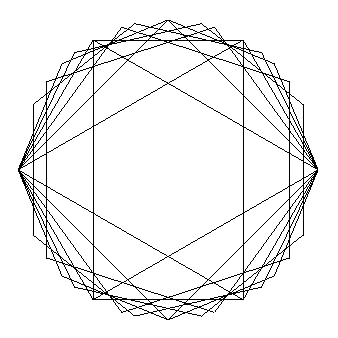
\includegraphics[width=1cm]{img/polygons}
\end{wrapfigure}

据我所知,包\textsf{wrapfig}并未
以提供\dm{dvi}文件的形式给出文档。
相反,可以在……
\end{verbatim}
\end{dmd}

\begin{wrapfigure}{r}{1.5cm}
  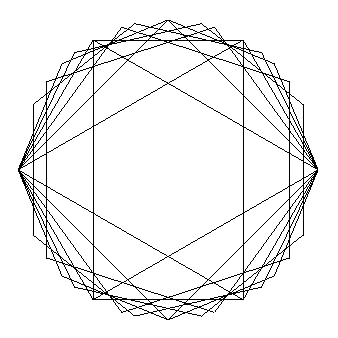
\includegraphics[width=1cm]{img/polygons}
\end{wrapfigure}

据我所知,包\textsf{wrapfig}并未以提供\dm{dvi}文件的形式给出文档。相反,可以在位于\dm{[...]/misc/wrapfig.stys}的\dm{.sty}文件自身中找到十分详细的信息。为了展示图片在段落中浮动带来的文字环绕效果,这段篇幅需要长一些,所以这里我多说一点:我们可以顺便注意到,借助一个著名的扩展——\textsf{docstrip},所有的包文档都可以“自动归纳”。这些扩展(extension),或者英文的\emph{package},包含其文档所需的代码,在安装过程中,会陆续被提取出来。\textsf{wrapfig}的作者八成没有遵循这个规则,可惜了……

\subsection{包\textsf{psfrag}}

另一个有趣的扩展是\textsf{psfrag}。它的目的是结合PostScript文件的强大和\LaTeX 方程的美观。我们想要在图片中集成数学式时,往往会遇到一个问题:大多数此类软件都不将支持数学方程作为预设。\textsf{psfrag}作者给出的解决方案中,可以使用指令\verb|\psfrag|在图中出现字符串的位置插入数学式。这样一来,使用以下方法即可生成图\ref{fig:5.3b}而非\ref{fig:5.3a}。
%此处源代码替换有问题,采用的解决方案来自https://zhidao.baidu.com/question/695901494124304244.html,即代码:
% \documentclass[border=2mm]{standalone}
% \usepackage{graphicx}
% \usepackage{psfrag}
% \begin{document}
% \psfrag{abc}{$\sin{a}$}%
% \includegraphics[width=5cm]{example.eps}
% \end{document}
% 然后执行 latex example; dvips example.dvi; epspdf example.ps
% 生成 example.pdf,在你的主文件中使用 \includegraphics{example.pdf} 导入。

\begin{figure}[ht]
  \begin{center}
      \leavevmode \subfloat[替换前]{%
        \label{fig:5.3a}
        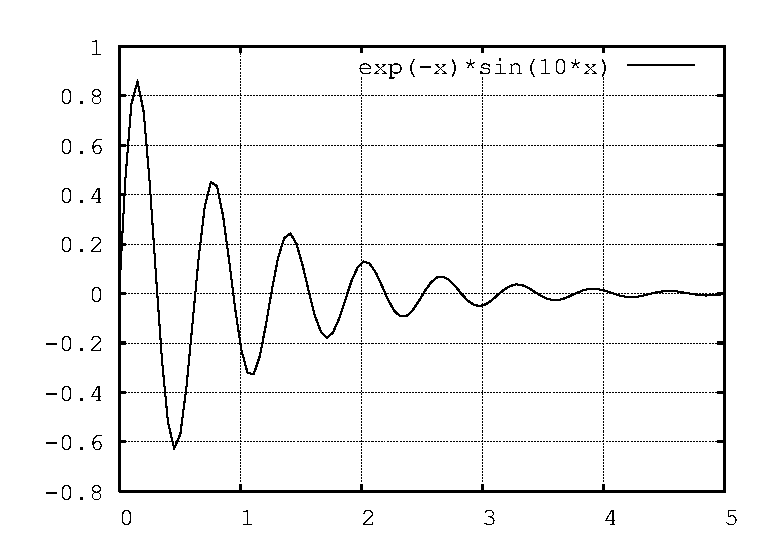
\includegraphics[width=0.4\linewidth]{img/courbe-sans-psfrag}}
      \hspace{2cm} \subfloat[替换后]{%
        \label{fig:5.3b}
        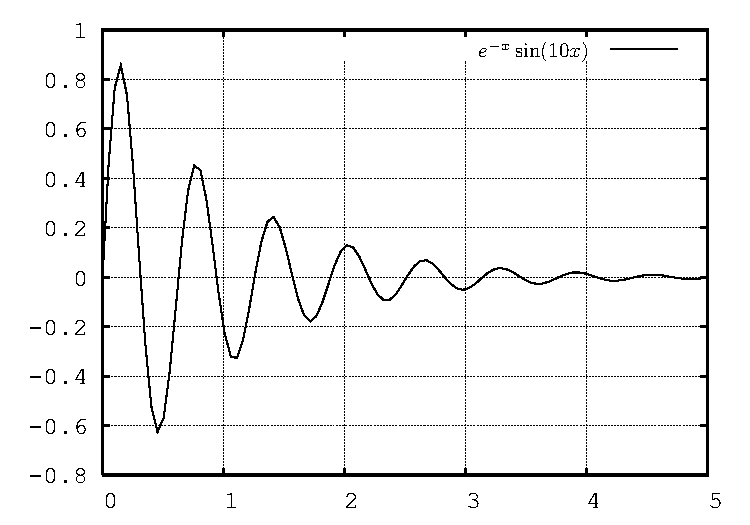
\includegraphics[width=0.4\linewidth]{img/courbe-avec-psfrag-replace}}
    \caption{\textsf{psfrag}的使用,右图中的\LaTeX 方程替换了左图的对应部分。}%TODO 分图引用不规范
    \label{fig:5.3}
  \end{center}
\end{figure}

\begin{enumerate}
  \item 在\verb+\includegraphics{courbe}+前添加一行代码:
  
  \begin{dmd}
  \verb+\psfrag{exp(-x)*sin(10*x)}[r][r]{$e^{-x}\sin(10x)$}+
  \end{dmd}
  
  该代码可以将图例中的字符串替换为漂亮的方程。
  \item 结果在\dm{.dvi}文件中不可见。相反,\textsf{dvips}会负责使用前面的指令来修改生成的PostScript文件。
\end{enumerate}

为公式确定位置的方法即为两个参考点确定位置,其中一个参考点来自方程,另一个来自需要替换的字符串。参考点的位置由用户通过指定指令\verb|\psfrag|中间的两个可选参数确定。假设我们像这样定义了参考点:

\begin{dmd}
\backslash psfrag\{字符串\}[l][c]\{\codereplace{数学方程}\}
\end{dmd}

这样的指令对应如下对其方式:

\newlength{\tempdimdemobox}

\newcommand{\chaine}{\dm{字符串}}
\newcommand{\ekouation}{\codereplace{数学方程}}

\newcommand{\contenu}[1]{%
  \ifthenelse{\equal{#1}{b}}{\raisebox{-5pt}[0pt]}{\raisebox{5pt}[0pt]}}

\newcommand{\point}[2]{% #1 (r ou l) #2 ($\bullet$ par ex.)
  \ifthenelse{\equal{#1}{r}}{%
    \setlength{\tempdimdemobox}{\fboxsep+.5\fboxrule}}{%
    \setlength{\tempdimdemobox}{-\fboxsep-.5\fboxrule}}%
  \makebox[0pt][l]{%
    \hspace{\tempdimdemobox}\makebox[0pt]{#2}}}

\newcommand{\boxdemo}[6][-5pt]{%
  \fbox{%
    \rule[#1]{0pt}{#2}%
    \ifthenelse{\equal{#3}{r}}{% point droite
      \contenu{#5}{\footnotesize#6}%
      \point{r}{#4}}{% sinon
      \ifthenelse{\equal{#3}{l}}{% point gauche
        \point{l}{#4}%
        \contenu{#5}{\footnotesize#6}}{% sinon
        \settowidth{\tempdimdemobox}{\footnotesize#6}%
        \makebox[0pt][l]{%
          \hspace{.5\tempdimdemobox}\makebox[0pt]{#4}}%
        \contenu{#5}{\footnotesize#6}}}}}%大括号随意转行会造成空格计入方框宽度

\begin{center}
  \newlength{\zob}
  \settowidth{\zob}{\boxdemo{14pt}{c}{$\bullet$}{t}{\chaine}}
  \boxdemo{14pt}{c}{$\bullet$}{t}{\chaine}\quad 和\quad
  \boxdemo[-7pt]{18pt}{l}{$\odot$}{b}{\ekouation} \quad 叠加的结果为 \quad
  \boxdemo{14pt}{c}{$\bullet$}{t}{\chaine}\kern-.5\zob\kern-.5\fboxrule%此行对比原书有改动
  \boxdemo[-7pt]{18pt}{l}{$\odot$}{b}{\ekouation}
\end{center}

同样地,如果使用如下指令:

\begin{dmd}
  \backslash psfrag\{字符串\}[r][l]\{\codereplace{数学方程}\}
\end{dmd}

则有如下结果:

\begin{center}
  \boxdemo{14pt}{l}{$\bullet$}{t}{\chaine}\quad 和\quad
  \boxdemo[-7pt]{18pt}{r}{$\odot$}{b}{\ekouation} \quad 叠加的结果为 \quad
  \boxdemo[-7pt]{18pt}{r}{$\odot$}{b}{\ekouation}\kern-\fboxrule%
  \boxdemo{14pt}{l}{$\bullet$}{t}{\chaine}
\end{center}

在图\ref{fig:5.3b}中,我们使方程的右侧(第一个可选参数为\dm{r})与原字符串的右侧(第二个可选参数为\dm{r})对齐。该包的文档十分具有参考价值……

\begin{exclamation}
注意,如果我们使用\LaTeX 源码生成PDF文件,则只能以使用一些扭曲的操作(参见\S A%TODO
)为代价来使用包\textsf{psfrag}。
\end{exclamation}

\subsection{包\textsf{xcolor}}

扩展\textsf{xcolor}由包\textsf{graphicx}的开发团队开发,在生成彩色文本时可能会很有趣——例如,生成带有透明度的颜色。包\textsf{xcolor}可以生成以下结构:

\begin{codelist}[5.6]{
  {一些\color{red}红色}和\textcolor{cyan}{青色}的文本。

  一个\colorbox{green}{绿色}字盒。
  
  另一个\fcolorbox{blue}{yellow}{字盒}。
}\begin{verbatim}
{一些\color{red}红色}和\textcolor{cyan}{青色}的文本。

一个\colorbox{green}{绿色}字盒。

另一个\fcolorbox{blue}{yellow}{字盒}。
\end{verbatim}
\end{codelist}

在这里,我们可以理解指定颜色的方法。

\begin{itemize}
  \item 使用声明:
  
  \begin{dmd}
    \backslash color\{\codereplace{颜色}\}
  \end{dmd}

  \item 使用指令:

  \begin{dmd}
  \backslash textcolor\{\codereplace{颜色}\}\{\codereplace{文本}\}
  \end{dmd}
\end{itemize}

类似地,对于字盒,有以下方法指定颜色。

\begin{itemize}
  \item 无边框:
  
  \begin{dmd}
    \backslash colorbox\{\codereplace{填充颜色}\}\{\codereplace{内容}\}
  \end{dmd}

  \item 有边框:
  
  \begin{dmd}
    \backslash fcolorbox\{\codereplace{边框颜色}\}\{\codereplace{填充颜色}\}\{\codereplace{内容}\}
  \end{dmd}
\end{itemize}

以上两个指令生成的彩色字盒对于长度\verb|\fboxsep|比较敏感。“如果颜色没有名字\emph{怎么办}?”我听到你在\emph{嘟囔}什么了……对于这个问题,我可以马上回答:

\begin{codelist}[5.7]{
  这是
{\color[rgb]{.2,.4,.5}\bfseries 
 蓝灰色}……
}\begin{verbatim}
这是
{\color[rgb]{.2,.4,.5}\bfseries 
 蓝灰色}……
\end{verbatim}
\end{codelist}

也可以为上例中的颜色起一个“小名”:

\begin{codelist}[5.8]{
  \definecolor{bleugris}{rgb}{.2,.4,.5}
这是
{\color{bleugris}\bfseries 蓝灰色}……
}\begin{verbatim}
\definecolor{bleugris}{rgb}{.2,.4,.5}
这是
{\color{bleugris}\bfseries 蓝灰色}……
\end{verbatim}
\end{codelist}

\begin{ii}
可以注意到,除了使用“\dm{rgb}”色彩模型,也可以使用定义灰度的\dm{gray}模型。同样地,如果使用\dm{html}模型,则可以使用HTML语法来指定颜色。
\end{ii}

\begin{figure}
  \centering TODO缺图%TODO
  \caption{推荐使用的储存图像文件树状结构:图像存储在一个目录中,矢量图存储在一个目录中,EPS格式的文件存储在另外的目录中}
  \label{fig:5.4}
\end{figure}

\section{使用\textsf{make}}

\begin{exclamation}
本节面向使用部署了GNU Make(更多有关信息,请参阅相关必读资料[11])的操作系统的用户准备的。其他人可以跳过这段学习路径……
\end{exclamation}

makefile使生成过程自动化的思路有:

\begin{itemize}
  \item 使用“位图”图像文件生成EPS格式的文件;
  \item 使用带有矢量绘图软件内置格式的文件生成EPS格式的文件。
\end{itemize}

为了实现以上思路,我们需要树立一个目标,可以用以下命令行表示:

\dmh{make figs}

假设图片和图像文件分别存储在主文件所在目录下的子目录\dm{Imgs}和\dm{Figs}中,生成的EPS文件同样存储在子目录\dm{Epss}中(如图\ref{fig:5.4}所示)。此时,就可以开始定义一系列变量,来指明需要用到的不同目录:

\begin{mdframed}
\begin{verbatim}
FIGSDIR=Figs
EPSSDIR=Epss
IMGSDIR=Imgs
\end{verbatim}
\end{mdframed}

\subsection{图像转码}

首先,(作为示例)我们列出JPEG和PNG格式文件的列表,使用如下两个变量来储存列表:

\begin{mdframed}
\begin{verbatim}
PNGS=$(notdir $(wildcard $(IMGSDIR)/*.png))
JPGS=$(notdir $(wildcard $(IMGSDIR)/*.jpg))
\end{verbatim}
\end{mdframed}
  
使用函数\dm{wildcard}可以获得文件夹\verb|$(IMGSDIR)|中文件的列表,而对于每个文件,函数\dm{notdir}可以删除其“目录”的部分。最终,变量\dm{PNGS}包含:

\begin{dmd}
i.png j.png
\end{dmd}

变量\dm{JPGS}包含:

\begin{dmd}
k.jpg
\end{dmd}

接下来,我们可以从这两个变量除法,创建即将生成的EPS文件的列表(再提醒一次,EPS文件应当单独存放在一个目录中):

\begin{mdframed}
\begin{verbatim}
IMGS2EPSS=$(patsubst %,$(EPSSDIR)/%,\
          $(PNGS:.png=.eps) $(JPGS:.jpg=.eps))
\end{verbatim}
\end{mdframed}

赋值符号右侧的表达式可以将前文中两个列表中文件的扩展名改为\dm{eps},并且文件名前加上存储EPS文件的目录作为前缀。因此,\dm{IMG2EPSS}包含:

\begin{dmd}
Epss/i.eps Epss/j.eps Epss/k.eps
\end{dmd}

该列表构成了(\textsf{make}意义上)生成图像的“先决”条件。因此,按以下方式定义目标:

\begin{mdframed}
\begin{verbatim}
figs : $(IMGS2EPSS)
\end{verbatim}
\end{mdframed}

此外,也需要向\textsf{make}解释我们如何将图像文件转换为封装好的PostScript格式。可以通过如下规则描述:

\begin{mdframed}
\begin{tabbing}
\verb|abcd|\=\kill
\verb+$(EPSSDIR)/%.eps : $(IMGSDIR)/%.png+\\
$\longmapsto$\>\verb+convert $< EPS:$@ +\\
\verb+$(EPSSDIR)/%.eps : $(IMGSDIR)/%.jpg+\\
$\longmapsto$\>\verb+convert $< EPS:$@+
\end{tabbing}
\end{mdframed}

这样的规则详细描述道:我们将会用到工具\textsf{convert}\jz{
  其属于包ImageMagick,可以在\wz{http://www.imagemagick.org}获取。该工具几乎可以转换所有格式的图片。
}来将JPEG和PNG文件转换为EPS格式。

\subsubsection{转换图像文件}

图像文件的转码严格遵循同一原则。假设我们指明了一个由\textsf{xfig}生成的fig格式源文件和一个由\textsf{Inkscape}生成的svg格式源文件,则\dm{makefile}有:

\begin{mdframed}
\begin{verbatim}
FIGS=$(notdir $(wildcard $(FIGSDIR)/*.fig))
SVGS=$(notdir $(wildcard $(FIGSDIR)/*.svg))
FIGS2EPSS=$(patsubst %,$(EPSSDIR)/%,\
          $(FIGS:.fig=.eps) $(SVGS:.svg=.eps))
\end{verbatim}
\end{mdframed}

当然,两条转换规则是不同的,因为它们分别会调用\textsf{fig2dev}(\textsf{xfig}的相关工具)和\textsf{Inkscape}本身:

\begin{mdframed}
\begin{tabbing}
\verb|abcd|\=\kill
\verb+$(EPSSDIR)/%.eps : $(FIGSDIR)/%.fig+\\
$\longmapsto$\>\verb+fig2dev -L eps $< > $@+\\
\verb+$(EPSSDIR)/%.eps : $(FIGSDIR)/%.svg+\\
$\longmapsto$\>\verb+inkscape -E $@ $<+
\end{tabbing}
\end{mdframed}

最终,用于输出图像文件和图片的目标如下:

\begin{mdframed}
\begin{verbatim}
figs : $(IMGS2EPSS) $(FIGS2EPSS)
\end{verbatim}
\end{mdframed}

\section{除此之外……}

针对特殊的需求,我们可以找到大量可以生成能满足需要的图像(电路图、直方图、树形图……)的扩展。实际上,你可能在某天需要使用一个指令自动生成若干图像,这时请看看可用的不同扩展(\textsf{pstricks}、\MP……)、环境\dm{picture}及其扩展\textsf{epic}和\textsf{eepic}。加油!

\begin{ii}
目前,包TikZ的发展顺风顺水。该包可以为其优秀的用户提供使用一种依赖\LaTeX 的语言创作图画的可能。如果文档中的图以等价的形式出现多次,这种解决方案会非常有趣。该包会在本书的未来版本中介绍\yz{
  我等到花儿也谢了……
}。
\end{ii}
\chapter{科技文档}

\begin{epigraphe}{《圣经·箴言》10:14}
    智慧人积存知识,\\愚妄人的口速致败坏。
\end{epigraphe}

现在,终于到了跟你聊聊所谓\emph{科技}文档特性的时刻。虽然关于数学式和其他方程的问题已经在第3章妥善解决,但还有一块骨头要啃:参考文献。对于这个问题,虽然不能一口吃个胖子,但接下来的内容可以让你大幅简化工作。在本章,我们还会解释生成索引的机制。

本章首先会介绍起草文章的几点特别之处,然后展示参考文献的生成和索引的生成,最后介绍将大篇幅文档拆解成几个小部分的实用方法。

\section{文章(article)}

为了起草一篇文章,没有什么新内容可以介绍的,我们目前为止见过的所有内容都适用。只需要注意,在文前部分中,可以使用以下指令:

\begin{itemize}
    \item \verb|\title|,定义标题;
    \item \verb|\date|,定义日期;
    \item \verb|\author|,定义作者团队;
    \item \verb|\thanks|,定义作者单位。
\end{itemize}

若要利用这些定义来插入标题,需要在\verb|\begin{document}|之\textbf{后}插入指令\verb|\maketitle|:

\begin{dmd}
\begin{verbatim}
\documentclass{article}
\title{Le seuillage à 128 : une révolution !}
\author{M. C. Orlanrien\\
        Institut du Pixel\\
        42007 Saint-Etienne---FRANCE}
\date{2 Avril 1927}
\begin{document}\end{verbatim}
\backslash maketitle\textsl{\% 标题插到此处}\\
...\\
\verb|\end{document}|
\end{dmd}

此处重复一遍\jz{
    因为传授知识就是重复的过程。
}:标题是由指令\verb|\maketitle|生成并插入的,而不是文前部分的定义。

通常来说,会议或期刊提供的模板文件中会引入一些变化(例如使用\verb|\address|分隔作者和其地址),但基本原理是一致的。

\section{参考文献}

由两种方式可以使用\LaTeX 起草文章的参考文献部分。其中,可以称得上是“手动”的方式是,在文章中插入环境\dm{thebibliography}。另一种方式,即此处要介绍的方式,是使用\bib ,主要分为如下步骤。

\begin{enumerate}
    \item 创建一个或多个参数文件,包含\bib 格式的各条参考文献入口(entrée;文章、会议……)。这个步骤不可避免地需要我们去\emph{输入}。
    \item 在文档中,使用指令\verb|\cite|去引用这些入口。
    \item 参考文献会自动根据你选择的特殊风格排版。
\end{enumerate}

这种方法的优势是,对于每条参考文献,你只需输入一次。此外,考虑到可以使用\emph{风格文件},你不用去担心它的版式。有几十种风格文件,对应各种标准,包含期刊和其他会议所使用的标准。我们也可以在互联网上找到\bib 格式的参考文献数据库,可以在文档中直接使用。

我们重复一遍:参考文献有多种标准。但不幸的是,一些期刊偏偏喜欢指定属于自己的参考文献格式。有朝一日你在这种期刊上发表文章时,就需要去创建或调整风格文件。为了实现这一点,可以去查找工具\textsf{makebst}。

\subsection{\dm{.bib}文件}

第一个操作是构建\jz{
    \textbf{Emacs}的Auc\TeX 组件包含了很好用的\bib 模式。
}参考文献文件,其扩展名最好为\dm{.bib}。该文件需要遵循特殊的语法。首先需要知道,\bib 通过\emph{类型(type)}区分每个入口。这样一来,每个入口都带有一个文档类型:图书、文章、会议、科技报告……一共有二十多种不用的文档类型。

\begin{ii}
正常来说,我们可以在伴随\LaTeX 发行版提供的文件找到名为\bib ing的文件(命名为\dm{btxdoc.pdf}),由奥兰·帕塔什尼克(Oran Patashnik)在约二十年前创作。该文件包含有关构建\bib 格式文件方法的重要信息来源。
\end{ii}

每个入口\emph{类型}都包含一定数量描述该入口的\emph{字段(champ)}。参考文件入口的结构如下:

\begin{dmd}
@\codereplace{入口}\{\codereplace{关键描述},\\
\verb|  |\codereplace{字段$_1$}\ =\ \{...\},\\
\verb|  |\codereplace{字段$_2$}\ =\ \{...\},\\
\verb|  |...\\
\verb|  |\codereplace{字段$_n$}\ =\ \{...\},\\
\}
\end{dmd}

其中,\codereplace{入口}表示文档类型(\dm{article}、\dm{inproceedings}等),\codereplace{字段$_1$}、\codereplace{字段$_2$}……\codereplace{字段$_n$}表示参考文献入口的不同字段。这些\bib 的保留字可以以大写或小写形式输入。

符号\codereplace{关键描述}需要以唯一方法描述该文档,以备通过用于识别标签的符号\verb|\label|来重新找到。为了你能够快速上手\bib ,接下来的示例综合了三个你需要使用的基本入口。

\subsubsection{期刊文章}

有一篇期刊文章需要以如下形式输入:

\begin{dmd}
\begin{verbatim}
@article{qtz:UchArb,
    author ={Uchiyama, Toshio and Arbib, Michael A.},
    title = {Color Image Segmentation
            Using Competitive Learning},
    journal=pami,
    volume =16, number=2, pages={1197--1206},
    month=dec, year=1994}\end{verbatim}
\end{dmd}

有以下几点需要注意。

\begin{enumerate}
    \item 字段\dm{author}、\dm{title}、\dm{journal}、\dm{year}是必需的。
    \item 对于作者\jz{
        此处关于作者的注意事项对于其他入口(会议、书等)也同样适用。
    }姓名,需要遵循\codereplace{姓}、\codereplace{名}的顺序。\textbf{所有}作者姓名都需要以\dm{and}分隔。
    \item 对于复合姓或其他特殊作者名,可以以如下形式输入:
    \begin{center}
        \dm{author="de la Motte Beuvron, Alain"}
    \end{center}
    其中遵循的顺序为:\codereplace{特殊组成部分}、\codereplace{姓}、\codereplace{名}。逗号作为分割符,起到与上例中相似的作用。
    \item 所有月份可以以字符串的形式给出,如\dm{jan}、\dm{feb}、\dm{mar}等。
\end{enumerate}


在\dm{.bib}文件的开头,为简洁起见,我们已经创建了\emph{缩写}\dm{pami}:

\begin{dmd}
\begin{verbatim}
@string{pami="IEEE transactions on Pattern Analysis and
              Machine Intelligence"}\end{verbatim}
\end{dmd}

\subsubsection{会议析出文章}

没错,\bib 会区分对待\emph{期刊}和\emph{会议}中的文章。格式结构与上例很相似,只不过\dm{booktitle}用于会议标题而不是期刊标题:

\begin{dmd}
\begin{verbatim}
@Inproceedings{qtz:BouOrch,
    author={Bouman, Charles A. and Orchard, Michael T.}
    title={Color Image Display with a Limited Palette Size},
    booktitle={SPIE Conference on Visual Communications
               and Image Processing},
    volume=1199,pages={522--533},
    year=1989}\end{verbatim}
\end{dmd}

这里,\dm{author}、\dm{title}、\dm{booktitle}、\dm{year}是必填字段,我们可以选用\dm{volume}和\dm{number}。

\subsubsection{图书片段}

相比于整本书,我们经常指参考其中的一个片段——若干章、若干页:

\begin{dmd}
\begin{verbatim}
@inBook{col:McA,
    author =    {MacAdam, David L.},
    title =     {Color Measurement},
    chapter =   4,
    pages   =   {48--49},
    publisher = {Springer-Verlag},
    year =      1985}\end{verbatim}
\end{dmd}

强制字段为:\dm{author}、\dm{title}、\dm{chapter}或\dm{pages}、\dm{publisher} (出版方),以及\dm{year}。

\begin{ii}
我们再次强烈建议你使用Emacs组件Auc\TeX 的\bib 模式。特别是该模式为你提供了包含所有入口类型的菜单。选择菜单中的一项,就可以在你的文件中插入入口“骨架”。该组件可以在\wz{ftp.lip6.fr/pub/TeX/CTAN/support/auctex}下载,也可以以包Debian的形式获取。
\end{ii}

\subsection{参考文献的标注}

一旦参考文献建立完成,就可以即刻在文档中借助关键描述使用指令\verb|\cite|来标明引用:

\begin{dmd}
\backslash cite\{\codereplace{关键描述}\}
\end{dmd}

指令\verb|\cite|有如下功能:

\begin{enumerate}
    \item 根据选择的风格插入跳转符号(如[2]、[Loz95]等);
    \item 在文档的参考文献部分中添加所引用的文章。
\end{enumerate}

\begin{ii}
    文章(此处指广义的文章)只有在被\verb|cite|作为引用对象时才会出现在参考文献中。若要列出未于正文中直接引用的文章,则需要使用指令\verb|\nocite{|\codereplace{关键描述}\verb|}|将\codereplace{关键描述}的对应文章插入文档的参考文献部分。此外,指令\verb|\nocite{*}|会将\dm{.bib}文件中的\emph{所有}入口插入文档。
\end{ii}

在实际进入生成参考文献的步骤前,需要在\LaTeX 文档末尾添加对以下指令的引用来指定参考文献的风格:

\begin{dmd}
\verb|\bibliographystyle|
\end{dmd}

然后,引用如下指令来实际插入参考文献:

\begin{dmd}
\verb|\bibliography|
\end{dmd}

对于风格,有:

\begin{dmd}
\backslash bibliographystyle\{\codereplace{风格}\}
\end{dmd}

\LaTeX 预定义的风格\jz{
    在CTAN网站的\dm{biblio/bibtex/contrib}可以找到几十种可供使用的其他风格。
}如下。

\begin{itemize}
    \item \dm{plain},引用的形式为[2],参考文献会根据作者名排序。
    \item \dm{unsrt},参考文献根据引用顺序排序。会议文章经常使用这种风格。
    \item \dm{alphs},引用的形式为“作者缩写+年份”。
\end{itemize}

接下来,需要指定哪些文件包含了文档中指令\verb|\cite|所“指向”的那些参考文献:

\begin{dmd}
\backslash bibliography\{\codereplace{文件$_1$}, \codereplace{文件$_2$}, \codereplace{……}\}
\end{dmd}

这样的指令会使\bib 在处理过程中包含\codereplace{文件$_1$}\dm{.bib}、\codereplace{文件$_2$}\dm{.bib}……

\subsection{生成参考文献}

生成参考文献的步骤如下。

\begin{enumerate}
    \item 借助\LaTeX 实现第一次编译,使得辅助文件\dm{doc.aux}包含\emph{引用标注}信息:
    
    \begin{center}
        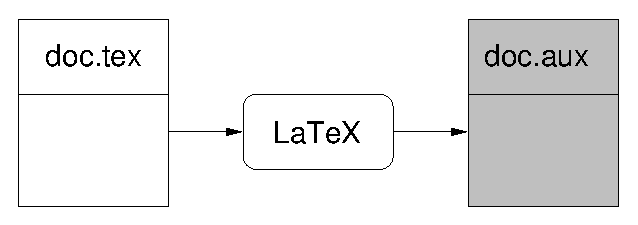
\includegraphics{img/bibtex1}
    \end{center}
    
    \item 运行\bib ,在文件\dm{doc.bbl}中生成参考文献:
    
    \dmh{bibtex doc}

    \begin{center}
        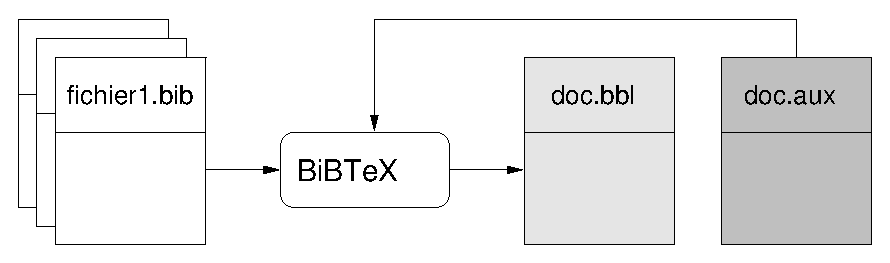
\includegraphics{img/bibtex2}
    \end{center}

    \item 借助\LaTeX 的第二次编译插入参考文献:
    
    \begin{center}
        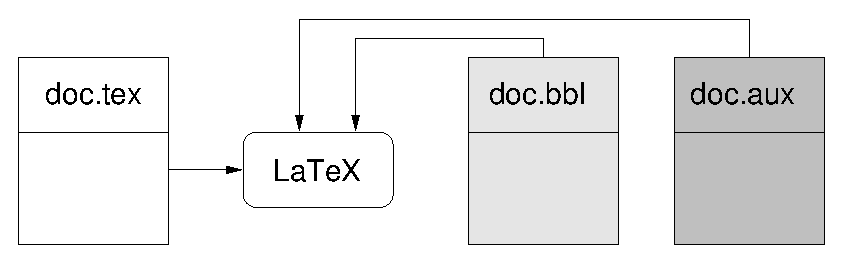
\includegraphics{img/bibtex3}
    \end{center}

    %TODO 图片中bibtex和latex替换

    \item 通过第三次编译解析交叉引用。
\end{enumerate}

如果你对这个过程感到好奇,可以看到:文件\dm{doc.bbl}包含了环境\dm{thebibliography}以供随时使用\jz{
    也就是说,你如果不使用\bib ,就必须着手处理该环境。
};文件\dm{doc.blg}是与那些\dm{.log}文件相似的“日志”文件,储存着上一次使用\bib 时一些可能出现的错误或警告。

\begin{exclamation}
程序\bib 对环境\dm{BIBINPUTS}中的参数敏感。因此,在某些情况下,有必要在\linebreak\dm{.bash\_profile}中添加以下一行命令:

\dmh{export BIBINPUTS=\$HOME/LaTeX/biblio//:}

这样可以使\bib 在目录\dm{\$HOME/LaTeX/biblio}中搜索你的参考文献文件(此处的目录为示例)。
\end{exclamation}

\section{索引}

生成索引需要依靠以下两个概念:

\begin{enumerate}
    \item 在\LaTeX 文档中添加指令\verb|\index|来添加索引入口;
    \item 使用程序\textbf{makeindex}来正确地抽取和展示索引。
\end{enumerate}

负责在文档中插入索引部分的是指令\verb|\printindex|。可以将该指令与\verb|\tableofcontents|类比。

\subsection{必要步骤}

这里给出简短的索引制作备忘录:

\begin{enumerate}
    \item 在主文件中插入两条指令:
    \begin{dmd}
    \begin{tabbing}
12345678902234567890\=\kill
\verb|\makeindex|\>\textsf{$\leftarrow$告知\LaTeX 需要生成索引}\\
\verb|\begin{document}|\\
{\rmfamily ……文档正文……}\\
\verb|\printindex|\>\textsf{$\leftarrow$在文档中实际插入索引部分}\\
\verb|\end{document}|
    \end{tabbing}
    \end{dmd}

    \item 插入索引入口:
\begin{dmd}
\begin{tabbing}
12345678902234567890\=\kill
\verb|\index{bidule}|\>\textsf{$\leftarrow$在索引中插入“bidule”}
\end{tabbing}
\end{dmd}

    \item 为了为文档\dm{doc.tex}生成索引,需要成功执行以下三条指令:
    
    \begin{dmd}
        latex doc\\makeindex doc\\latex doc
    \end{dmd}
\end{enumerate}

\subsection{机制细节}

文档\dm{doc.tex}的第一次编译(在满足文前部分带有控制序列\verb|\makeindex|的条件下)会生成包含“散装”的索引入口文件\dm{doc.idx}:

\begin{center}
    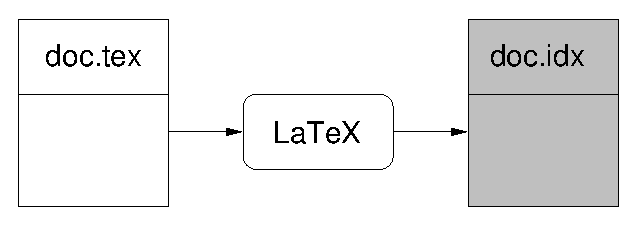
\includegraphics{img/makeindex1}
\end{center}

接下来,使用\textsf{makeindex},在这个文件\dm{doc.idx}中整理条目、删除重复项,并将结果存入\dm{doc.ind}。执行轨迹会存储在\dm{doc.ilg}中:

\begin{center}
    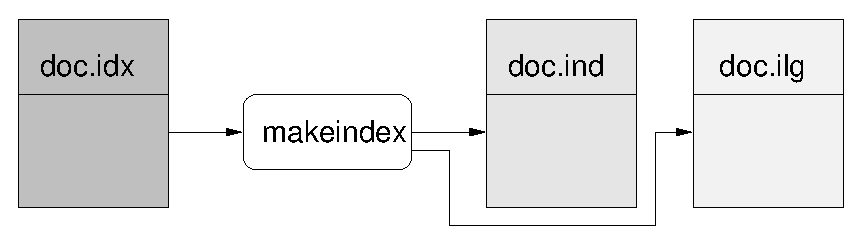
\includegraphics{img/makeindex2}
\end{center}

终端下运行的\textsf{makeindex}嘴很碎。如下展示了它生成文档索引时展示的信息:

\begin{dmd}
\begin{verbatim}
This is makeindex, version 2.13 [07-Mar-1997] (using kpathsea).
Scanning input file guide.idx....done (982 entries accepted, 0 rejected).
Sorting entries...........done (11254 comparisons).
Generating output file guide.ind....done (745 lines written, 0 warnings).
Output written in guide.ind.
Transcript written in guide.ilg.\end{verbatim}
\end{dmd}

因此,在运行失败的情况下,需要警惕可能出现的抛出和警告(\emph{warning})。\LaTeX 的第二次编译可以在\dm{doc.tex}中指令\verb|\printindex|指出的位置插入格式化过的索引(文件\dm{doc.ind}):

\begin{center}
    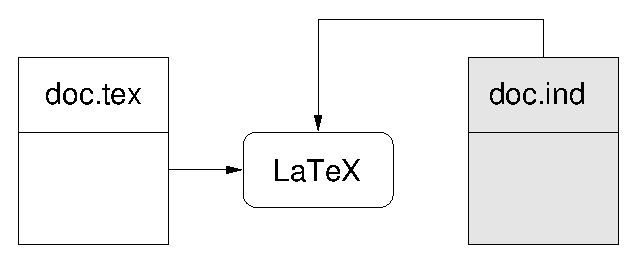
\includegraphics{img/makeindex3}
\end{center}

\begin{ii}
工具makeindex可以识别选项\dm{-s},该选项用于为索引指定\emph{风格}。这里所说的风格定义在带有扩展名\dm{.ist}的文件中,可以改变索引的排版央视。可以以如下方式修改文件风格:

\dmh{makeindex -s}\codereplace{文件风格}\codereplace{主文件}

可以在你使用的发行版中寻找风格文件并测试它们。
\end{ii}

\subsection{索引入口的不同类型}

目前为止,我们看到的索引形式都是\emph{\codereplace{索引词}及\codereplace{页码}},但也可以使用更讲究些的入口形式,至少包含如下三种。

\begin{enumerate}
    \item 带有层级的入口:
    
    \begin{dmd}
    \verb|\index{bidule!chouette}|
    \end{dmd}

    该指令可以在索引中插入“bidule”的子入口“bidule”。

    \item 跨页入口:
\begin{dmd}
\begin{tabbing}
12345678902234567890\=\kill
\verb+\index{bidule|(}+\>\textsf{$\leftarrow$位于第$i$页}\\
\verb+\index{bidule|)}+\>\textsf{$\leftarrow$位于第$j$页}
\end{tabbing}
\end{dmd}
    该指令插入的索引形式为bidule $i$--$j$。

    \item 符号化的入口:
    
    \begin{dmd}
    \verb|\index{alpha@\alpha}|
    \end{dmd}

    这样的指令会在索引中插入$\alpha$,并按“alpha”将其分类。同样地,以下指令会在索引中插入“épluche”,但分类时会将首字母看作“e”:

    \begin{dmd}
    \verb|\index{eplucher@éplucher}|
    \end{dmd}
\end{enumerate}

此处列出的最后一个格式同样可以用于为索引插入带有特殊版式的入口。例如:

\begin{dmd}
\verb|\index{bonjour@\textbf{bonjour}}|
\end{dmd}

该指令可以在索引中插入\textbf{bonjour}(即将bonjour加粗),同时按“bonjour”将该入口分类。此外,借助以下指令,我们还可以以特殊版式显示页码:

\begin{dmd}
\backslash index\{\codereplace{入口}|\codereplace{版式指令}\}
\end{dmd}

例如:

\begin{dmd}
\verb+\index{bidule|textbf}+
\end{dmd}

该指令可以让索引中“bidule”的页码显示为加粗样式(注意,在版式指令中没有符号\verb|\|)。

\subsection{术语词典}

有时,我们需要详细列出文档中一些术语的含义。文档中重新组织这些术语解释的部分称为\emph{术语词典(glossaire)}。为了生成术语词典,需要采用与生成\celan{\S 6.3.1}索引相似的方法,只需做一些小的改动,将在11.6节详细介绍。

\section{拆分文档}

如果文档的篇幅很长,我们可以将其自然地按章或部分来拆解。因此,建议创建一个\emph{主}文档,并在其中包含各章或各部分。主文档的形式如下:

\begin{dmd}
\begin{verbatim}
\documentclass{book}

\begin{document}\end{verbatim}
\verb+\frontmatter +\textsl{\% 所有介绍性的文字}
\begin{verbatim}
\include{preface}
\tableofcontents\end{verbatim}
\verb+\mainmatter +\textsl{\% 文档的“主体”}
\begin{verbatim}
\part{关于\LaTeX 的那些你想知道却从不敢问的问题}

\chapter{基本原则}
\begin{quote}
    人若身患漏症,他因这漏症就不洁净了。——《圣经·利未记》15:2
\end{quote}

本章介绍\LaTeX 的基本原理。你将会看到关于\LaTeX 安装的简介、使用\LaTeX 的基本“流程”(session)介绍、文章格式的结构、使用变音符号的注意事项,认识几个工具,以及了解面对编译错误消息时的态度。

\section{安装}

你想安装\LaTeX 吗?你将要安装的是\LaTeX 的其中一个\textit{发行版},具体的版本取决于你的操作系统\jz{
    如果你不知道操作系统是什么东西,那么你使用的是macOS;如果你不知道你的计算机用的\textit{具体是哪个}操作系统,那么你在用Windows;否则,你在用UNIX……
}。发行版中带有可以自动安装和配置\LaTeX 、\TeX 和其他相关内容的程序。

\paragraph*{对于UNIX}我们可以找到称为te\TeX 的发行版,虽然它的开发早在2006年就停止了。今天,我们一般安装\TeX Live(\wz{http://www.tug.org/texlive})。

\paragraph*{对于macOS}建议安装的发行版是Mac\TeX(\wz{http://www.tug.org/mactex})。

\paragraph*{对于Windows}最简单的方式无疑是选择pro\TeX t(\wz{http://www.tug.org/protext})。它会安装称为MiK\TeX 的发行版(\wz{http://www.miktex.org})和几个开发工具,其中包含一个查看PostScript文件的程序(\textsf{gsview})。

偶尔,需要在为发行版中搭配一款文字编辑器(如果其中没有包含),因为你很快就能看到,使用\LaTeX 就是在文件中输入文字和命令。

\begin{itemize}
    \item UNIX中,推荐使用\textsf{emacs}或\textsf{vi},即使前者明显比后者更高级,但二者用户之间无结果的恶意争吵仍在继续。
    \item \textsf{kile}和\textsf{texmaker}是已集成的开发环境。依靠它们,初学的用户在入门时会觉得更轻松。它们的特点是将编辑、编译和可视化集成在一个界面。这两个环境也使通过菜单、对话框或其他标签来探索\LaTeX 指令称为可能(如图\ref{fig:1.1}a所示)。
    \item Windows中的对应产品是\textsf{\TeX nicCenter}(如图\ref{fig:1.1}b所示)。
    \item macOS中的对应产品是\textsf{\TeX shop}和\textsf{i\TeX max}。
\end{itemize}

\begin{figure}%[H]
    %TODO 图
    \centering
    \includegraphics[width = 0.8\linewidth]{img/kile.eps}\\
    (a) Kile\\
    \includegraphics[width = 0.8\linewidth]{img/texniccenter.eps}\\
    (b) \TeX nicCenter
    \caption{集成的两个开发环境:Linux中的Kile和Windows中的\TeX nicCenter。它们将编辑、编译和可视化集成在一个界面中}
    \label{fig:1.1}
\end{figure}

你很快就会学到,用\LaTeX 制作文档是一个翻译(也称作\textit{编译})的过程——将编辑者创建的源文件转换为用于显示或印刷的格式\jz{本章会略微多介绍一些这个格式。}。因此,发行版中内置了或多或少的著名工具,可以将编译后的不同格式的文件显示出来。

\paragraph*{对于PDF格式}除了著名的\textsf{acrobat reader},UNIX中还有一些可以显示PDF文件,如\textsf{xpdf}、\textsf{evince}等。

\paragraph*{对于DVI格式}UNIX中的\textsf{xdvi}、\textsf{kdvi}和Windows中的\textsf{yap}都是可以显示这种\LaTeX 编译文件的程序。

\paragraph*{对于PostScript格式}\textsf{ghostscript}套件(在各平台下的名称可能有差异)可以显示PostScript文件。

\begin{exclamation}
    需要注意,为了使你选用的发行版包含\LaTeX 的“法文”模式,以确保能够正确处理断字(césure;英:hyphenation),我们需要在编译文档是需要更改其“日志”(见1.6节)%带有引用
    以使法文模式加载:

    \begin{dmd}
    LaTeX2e <2005/12/01>\\
    Babel <v3.8h> and hyphenation patterns for english, [...] dumylang, \fbox{french}, loaded.
    \end{dmd}
\end{exclamation}

\section{“生产”周期}

即使\LaTeX 并不是通常意义上说的编译型语言,但我们仍然可以将制作一个\LaTeX 文档的周期与使用一款经典的编程语言开发软件的\textit{编辑—编译—执行}周期进行类比。

\subsection{编辑}

一个\LaTeX \textit{源}文件是一个文本文件\jz{即文件仅由组成其中符号的代码构成。}。因此,对\LaTeX 文件的操作并不依赖于某个特定的软件,只需要一个经典的文本编辑器即可。因此,若要操作\LaTeX 文档,指令

\dmh{emacs \codereplace{文件名}.tex \&} %TODO <>

或

\dmh{vi \codereplace{文件名}.tex}

足以让你进入\LaTeX 文档这个充满野性和未知的世界。在Windows中,根据自己的喜好,我们可以选用一款文字编辑器。注意,对于\LaTeX 源文件,推荐使用\dm{.tex}扩展名名。

\subsection{编译}

我们用如下指令开始编译:

\dmh{pdflatex \codereplace{文件名}.tex}

早晚有一天,你会看到编译会产出错误。这将是1.6节会处理的问题。总之,解决了编译问题后,我们会得到一个带有\dm{.pdf}扩展名的文件,它代表\textit{便携文件格式(英:portable document format)},这是一种由Adobe公司创造的著名格式。

\begin{ii}
    历史上,编译\LaTeX 源文件会生成\dm{dvi}文件,代表\textit{设备无关(英:device independant)}。此类文件独不受输出环境(如屏幕、打印机等)的影响。这是一种包含了“图像”的\LaTeX 便携二进制文件,可以用于各种操作系统。随后,出现了一批用途各异的程序:
    \begin{itemize}
        \item 用于显示文档,即\dm{.dvi}\rightarrow 点阵屏幕;
        \item 用于打印,即\dm{.dvi}\rightarrow 打印机语言;
        \item 用于转换格式,即\dm{.dvi}\rightarrow PostScript文件。
    \end{itemize}
\end{ii}

图\ref{fig:1.2}表明了UNIX生成最终文件过程中参与流程的多种程序。

\begin{ii}
    除了使用pdflatex外,也可以使用其他“编译器”来生成PDF文件。例如,xelatex和lualatex可以能正确地处理以UTF-8编码的文件,是常用的替代选项。
\end{ii}

\begin{figure}[H]
    %TODO 图
    \centering
    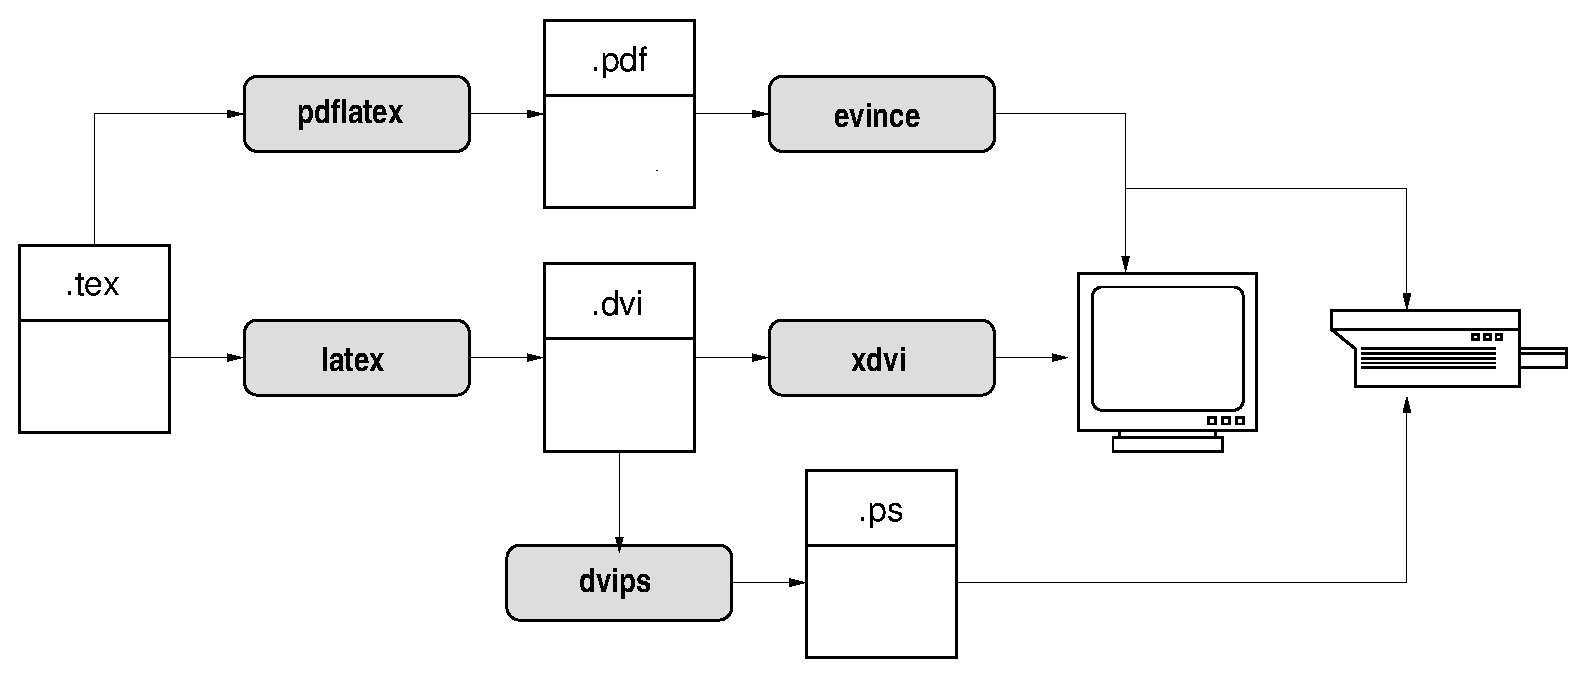
\includegraphics[width = 0.8\linewidth]{img/cycle.eps}
    \caption{UNIX中参与生成过程的工具}
    \label{fig:1.2}
\end{figure}

\subsection{显示}%visualisation有时翻译成可视化,有时翻译成显示,这个可以后期再统一一下。

在编译后,可以简单地使用\textsf{evince}程序来完成显示步骤。输入以下指令:

\dmh{evince \codereplace{文件名}.pdf \&}

这是一个\textsf{linux}下运行的十分直观的程序,能够给出一个方便阅读的文件预览。

\begin{exclamation}
    注意,不必在每次编译后都重新运行evince,它显示的内容会自动刷新。
\end{exclamation}

\subsection{打印}

对于\dm{pdf}格式,如何打印它这一问题就丢给了你的操作系统。关于这一点,没有特殊的注意事项。你有了一个文件,可以自由地处置它,无论是直接打印,还是根据你所处的环境来发挥才艺。

\begin{ii}
    从\dm{dvi}到\dm{ps}格式的转换需要调用dvips程序:

    \dmh{dvips \codereplace{文件名}.dvi}

    这可以生成一个PostScrpt格式的文件。这个格式也由Adobe创造,是一种打印机语言,可以看作\dm{pdf}的祖先。目前的打印机出厂即可识别这种打印机语言。我们可以说,文件发送到打印机时,十有八九传送的是PostScrpt格式的参数。对于PostScript格式的文件,有大量可以显示、修改这种文件的工具。
\end{ii}

\section{源文件的结构}

本节将介绍一种文档类型。实际上,所有\LaTeX 文档都具有相同的结构,形式如下:

\begin{dmd}
\backslash documentclass[\codereplace{类选项$_1$},\codereplace{类选项$_2$},...]\{\codereplace{类}\}\\
\backslash usepackage[\codereplace{包选项$_1$},\codereplace{包选项$_2$},...]\{\codereplace{包}\}\\
...\\
\codereplace{文前部分}\\
...\\
\backslash begin\{document\}\\
...\\
\codereplace{文本}\\
...\\
\backslash end\{document\}
\end{dmd}

如此一来,所有的\LaTeX 文档都可以按以下方式拆解。

\begin{itemize}
    \item 说明文档的\codereplace{类};
    \item 文前部分,包含以下内容:
        \begin{itemize}
            \item 使用特定的\codereplace{包};
            \item 多样的初始化和声明;
        \end{itemize}
    \item 文档主体,即我们将要亲手输入的全部内容,出现在\dm{\backslash begin\{document\}}和\dm{\backslash end\{document\}}之间。
\end{itemize}

以下介绍各部分的细节。

\subsection{文档的类}

所谓类,就是提供给\LaTeX 的一个指示,可以帮助\LaTeX 决定如何为文档的特定部分排版。根据具体使用的类不同,允许使用与否的指令可能不同(如\dm{\backslash chapter}在\dm{book}类中允许使用,在\dm{article}类中不允许使用)。另一方面,根据所选择的类,给出的命令会具有特定的含义(标题、材料表……)。在入门时\jz{
    实际上,我们可以在\dm{\backslash documentclass}前添加更多神奇的“咒语”……
},所有的\LaTeX 文档都必须以的指令开始——\dm{\backslash documentclass}接由花括号括住的类,包含以下几种:

\begin{itemize}
    \item \dm{article},用于文章;
    \item \dm{proc},用于电气与电子工程师协会(英:Institute of Electrical and Electronics Engineers,IEEE)会刊(英:proceeding)风格的文章;
    \item \dm{report},用于几十页篇幅的报告;
    \item \dm{book},用于图书或论文;
    \item \dm{letter},用于信件;
    \item \dm{slides},用于演示文档。
\end{itemize}

我们当然也可以为文档定义自己的类。类的配置项用方括号括住,可以是以下内容之一:

\begin{itemize}
    \item \dm{11pt, 12pt},用于全局地更改文字字号;
    \item \dm{twoside},用于生成适合双面打印的文档;
    \item \dm{draft},用于以草稿模式生成文档。
\end{itemize}

例如,输入:

\begin{dmd}
\verb|\documentclass{article}|
\end{dmd}

以上命令可以将全部配置项配置为默认值(字号为10 pt,单列,单面……)。

\begin{dmd}
    \backslash documentclass[12pt]\{article\}
\end{dmd}

以上命令将字号设置为12 pt(默认为10 pt)。再如:

\begin{dmd}
    \backslash documentclass[twoside, draft]\{report\}
\end{dmd}

以上命令可以以草稿模式生成适合双面打印的报告。

\subsection{文前部分}

文前部分是指位于子句\dm{\backslash documentclass}和子句\dm{\backslash begin\{documennt\}}间的区域。在这个区域中,我们可以明确想要包含的扩展(请看下一小节)%TODO
、初始化全局参数(如页边距等)、定义风格(如标题样式、序号等)、定义特殊的宏,等等。

\subsection{添加扩展}

\LaTeX 命令\dm{\backslash usepackage}可以与C语言的指令\dm{\#include}类比。这一命令允许添加\LaTeX 中满足宏或环境形式的功能\jz{
    相关内容将在下一章讲解。%TODO
}。目前,只需记住,我们可以在一行之内包含多个包:

\begin{dmd}
    \backslash usepackage\{\codereplace{包$_1$},\codereplace{包$_2$},\codereplace{包$_3$},...\}
\end{dmd}

如果\codereplace{包$_1$}、\codereplace{包$_2$}、\codereplace{包$_3$}拥有共同的配置项\codereplace{opt1},我们可以输入:

\begin{dmd}
    \backslash usepackage[\codereplace{opt1}]\{\codereplace{包$_1$},\codereplace{包$_2$},\codereplace{包$_3$}\}
\end{dmd}

相反,如果\codereplace{opt1}只涉及\codereplace{包$_2$},那么我们只能像这样写成两行:

\begin{dmd}
    \backslash usepackage\{\codereplace{包$_1$},\codereplace{包$_3$}\}\\
    \backslash usepackage[\codereplace{opt1}]\{\codereplace{包$_2$}\}
\end{dmd}

下面是两个例子:

\begin{dmd}
    \% 包graphicx带有配置项draft和xdvi\\
    \backslash usepackage[xdvi, draft]\{graphicx\}\\
    \% 包array和包subfig\\
    \backslash usepackage\{array, subfig\}
\end{dmd}

\begin{exclamation}
    根据定义,所有(类、包、命令的)的配置项参数都是\textit{可选的}。因此我们可以这样记:\LaTeX 中所有由方括号括住的参数\dm{[...]}都是非强制的。
\end{exclamation}

\section{开始!}

在本节,我们将尝试从一个只含几个排版命令的文档开始,介绍\LaTeX 的基本原理。

\begin{codelist}[1.1]{
    从你手中掉落的工具总是掉到最难够到的地方,或脆弱的物品上。\\
    这是\emph{墨菲}定律(loi de Murphy)的一个体现。
}  \begin{dmd}
    \verb+\documentclass{article}+\\
    \verb+\begin{document}+\\
    从你手中掉落的工具\\
    总是掉到最难够到的地方,\\
    或脆弱的物品上。\\
    ~\\
    \verb+这是\emph{墨菲}定律(loi de      Murphy)的+\\
    一个体现。\\
    \verb+\end{document}+
\end{dmd}
\end{codelist}

这个示例体现了\LaTeX 中的几个重要的原理,具体如下。

\paragraph*{空行代表跳转至下一段} \LaTeX 中的空行代表一段文字的结尾,因此在以上实例中,第一段从“\dm{从你}”开始,直到“\dm{物品上。}”结束。指令\dm{\backslash par}与空行等价,可以用来表示一段文字的起始。

\paragraph*{\LaTeX 会忽略换行}最终的文档中,换行并不由源文件中的换行决定。\LaTeX 会自动为各段文本\textit{打断、压缩、调节}文字,除非你有特殊的要求。

\paragraph*{\LaTeX 会忽略重复的空格}输入1个或18784个空格是等价的,比如源码中\dm{de}和\dm{Murphy}前插入的空格那样。此规则也适用于跳转段落:输入一行或多行空格是等价的。

\paragraph*{“\backslash ”是转义字符(caractère d’échappement;英:escape char)}“\backslash ”可以告诉\LaTeX 它后面的一系列字符是控制序列,也就是说,是最一般意义上的指令(或宏)。这里,它对“墨菲”一词生效,具体的效果由指令\dm{\backslash emph}控制。

\paragraph*{“\{”和“\}”}它们是\textit{组}的定界符,稍后会进一步解释它们。

\subsection{几个特殊字符}

就像符号“\backslash”的出现所暗示的那样,\LaTeX 中还有10个有特殊含义的符号,在此将其列出:

\begin{dmd}
    \verb+\ $ & % # ^ _ { } ~+
\end{dmd}

%todo 此前代码可以重新简化为verb

以下是一个使用部分特殊字符的案例:

\begin{codelist}[1.2]{
\textbf{是}下标:$x_{i+1}$,还是上标:$e^{i\pi}$;这是问题~1!
}\begin{verbatim}%毫无意义的段落
\textbf{是}下标:$x_{i+1}$,
还是上标:$e^{i\pi}$;
这是问题~1!%还是问题2?\end{verbatim}
\end{codelist}

目前,你需要知道:

\begin{itemize}
    \item \dm{\%}会使得\LaTeX 忽略当前行的剩余部分,因此,它是表示注释的符号(与C中的\dm{//}等价);
    \item \verb+~+代表不可拆分的空格\jz{
        见2.10节。
    },可以防止\LaTeX 在指定的位置断字。尽管有大量的情况需要插入这个符号来表示不可拆分(如所有形如“\verb+图~1+”的情况),然而,对于此类符号的使用,并没有系统化的规则。
    \item \dm{\$}用于标记公式的开始和结束。\LaTeX 遇到一个\dm{\$}符号时,它会切换到\celan{第3章}数学模式,直到遇到下一个\dm{\$}符号。
    \item \dm{\_}和\dm{\^{}}分别代表将文本转化为下标和上标。\textbf{注意},这两个符号只能在数学模式下使用。
    \item \dm{\{}和\dm{\}}分别表示组的开始和结束。本例中出现了两种组:一种出现在数学模式中,用于把将要放到下标或上标的“子公式”组合起来;另一种把将要设置成粗体的文字组合起来。
\end{itemize}

我们可以使用如下的指令来在让文档生成部分特殊字符:

\begin{dmd}
    \verb+\$ \& \% \# \{ \} \_+
\end{dmd}

这串指令可以输出“\$ \& \% \# \{ \} \_”。2.2.5小节%TODO
会解释如何使文档生成其余特殊字符(即\verb+\ ~ ^+)。

\subsection{调用指令}

你已经知道了,要想调用指令或宏,需要输入转义字符,并紧接着输入你想使用的宏名。%TODO 二对一
但是,\LaTeX 如何知道宏名的末尾在哪里呢?此处以用于生成\TeX 标识的\dm{\backslash TeX}为例来解释\yz{
    此例涉及对西文行文中空格的处理,不宜翻译。
}。

\begin{codelist}{
    \TeX book is for \TeX hackers.

    \TeX\  has some powerful macros.

    \LaTeX{} is a document preparation system
}\begin{verbatim}\TeX book is for \TeX hackers.

\TeX\  has some powerful macros.

\LaTeX{} is a document preparation system
    \end{verbatim}
\end{codelist}

\begin{exclamation}
    \verb*|\ |(其中\verb*| |代表空格)称作控制空格(espace de contrôle)。这个空格不会被\LaTeX 忽略。因此,指令“\verb*|et\ \ \ hop !|”会生成“et\ \ \ hop !”。实际上,以\dm{\backslash}\codereplace{函数}\dm{\{}\codereplace{参数}\dm{\}}的形式来调用宏是很好的习惯。因此,使用上例中的的第三种方式比第二种方式更佳。这种形式可以避免空格被忽略的情况发生\jz{
        所以他为什么要跟我们说这些?!
    }。因此,我们将使用\verb|the \teX{}book|来生成“the \TeX{}book”,使用“\verb*|\LaTeX{} is a ...|”来生成“\LaTeX{} is a ...”。
\end{exclamation}

\subsection{变音符号}

法国人往往对于使用\LaTeX 这件事忧心忡忡,因为法文中带有变音符号。别怕!你不必像表\ref{tab:1.1}\yz{
    该表与原书不完全相同。
}中展示的那样输入带有变音符号的字符。然而,你需要知道:无论是什么种类的字符,包括大写字母,我们都可以为其添加变音符号。

\begin{table}[H]
    \centering
    \begin{tabular}{|c|c|c|}
        \hline
        变音符号 & 源码 & 效果\\
        \hline
        尖音符 & \verb|\`z| & \`z \\
        钝音符 & \verb|\'z| & \'z \\
        长音符 & \verb|\^z| & \^z \\
        软音符 & \verb|\c{z}| & \c{z}\\
        分音符 & \verb|\"{z}| & \"{z}\\
        \hline
    \end{tabular}
    \caption{输入占7位(bit)的变音符号}
    \label{tab:1.1}
\end{table}

注意!虽然我们可以输入带有变音符号的字符,但不要忘记:这需要我们调用编码。目前,编码可能只针对地球上的某个地区。在法国,我们使用ISO 8859编码,配合拉丁文1区拓展。这套编码允许我们操纵美丽的变音符号。在详细阅读本书中专为使用法文书写文档的情况准备的章节\celan{第7章}之前,我们建议你在你源码的文前部分添加以下指令,以“攻克”法文文档的难关:

\begin{dmd}
    \begin{verbatim}
%源文件编码
\usepackage[latin1]{inputenc}
%TeX字体编码
\usepackage[T1]{fontenc}
%针对法文文档
\usepackage[francais]{babel}
    \end{verbatim}
\end{dmd}

\section{第一批工具}

以下几个宏和合字在文档中很常用,因此应当了解它们。首先,\LaTeX 会区分三种连接号:

\begin{itemize}
    \item \verb|-|,用于“Saint-Étienne”;
    \item \verb|--|,用于“page 12--24”;
    \item \verb|---|,在法文中用于插入语,如“une parenthèse --- comme cela”。
\end{itemize}

引号应以如下方式输入:

\begin{itemize}
    \item \verb|``|和\verb|''|可以输入英文中的引号\yz{
        此处与原书不同。原书前文输入变音符号时亦直接使用了单弯引号‘和’,但这两个符号作为命令参数时会导致编译错误,因此分别替换为反引号和直单引号。这可能是编译器的差异导致的。
    }——``English''。
    \item 如果键盘允许,对于法文,你可以输入«和»\jz{
        例如,在Linux系统下,分别按键盘的\fbox{Alt Gr}+\fbox{Z}和\fbox{Alt Gr}+\fbox{X}组合键(译注:适用于AZERTY键盘)。
    }。\textsf{babel}包的法文支持部分(参考第7章)%TODO
    允许我们通过\verb|\og|和\verb|fg|输入引号,由此,\verb|\og français\fg{}|这类命令是允许的—— «~français~»~。
\end{itemize}

以下是其余几个使用的命令:

\begin{itemize}
    \item \verb|\today|可以生成(编译时的)日期——2013年11月22日。
    \item \verb|\S|可以生成段落符号——\S。
    \item \verb|\ldots|可以在英文文档中生成省略号“\ldots”。但在法文文档中,应当输入三个点“...”(第7章会介绍更多有关法文排版的内容)。%TODO
\end{itemize}

最后要记得,英文中的双成分标点(ponctuation double;包括:;!?)前不加空格,但法文相反,它们的前面需要加空格。另外,在法国这个可爱的国家,我们几乎都靠右行驶。

\section{第一组报错}

\begin{ii}
    接下来,我们会看看\LaTeX 编译你的文档时闹的“情绪”。当我们放出编译指令时,我们会直接在终端看到这些输出。为了能让\LaTeX 得到充分使用,我们鼓励你在自己的环境下找到属于你自己的检查\LaTeX “\textsf{日志}”的方法。这些日体可以为你指明错误信息,以及编译过程中出现的其他警告。
\end{ii}

\subsection{症状}

如果你与\LaTeX 打交道,那么早晚有一天,你会看到屏幕上显示出类似这样粗旷的信息:

\begin{dmd}
    \linenumbers
    \begin{verbatim}
This is TeX, Version 3.1415 (C version 6.1)
(erreur.tex
LaTeX2e <1995/12/01>
(/usr/local/lib/texmf/tex/cls/article.cls
Document Class: article 1995/11/30 v1.3p Standard LaTeX document class
(/usr/local/lib/texmf/tex/clo/size10.clo)) (erreur.aux)
! Undefined control sequence.
l.5 paragraphe de ce \empha
                           {document}
?\end{verbatim}
\end{dmd}

几乎可以肯定,你看不懂这团内容。它是使用\LaTeX 处理文件\dm{erreur.tex}后终端上显示的内容。以下是文件全文\yz{
    文件正文意为:\dm{我觉得,在这样短的\backslash empha\{文档\}的第一段就有一个错误}。
}:

\begin{dmd}
    \begin{verbatim}
\documentclass{article}

\begin{document}
Il me semble bien qu’il y ait une erreur dans le
premier paragraphe de ce \empha{document} somme
toute assez court.
\end{document}
    \end{verbatim}
\end{dmd}

\subsection{诊断}

我们可以以一种简单的方式来解释以上错误信息。

\paragraph*{第1行}你使用的\TeX 版本为$\pi\pm 10^{-4}$。
\paragraph*{第2行}你想编译文件\dm{erreur.tex}。
\paragraph*{第3行}你使用了\LaTeXe ,版本日期为1995年12月。
\paragraph*{第4行~第5行}你使用了标准文档类\dm{article}。
\paragraph*{第6行}字号默认设置为10 pt。
\paragraph*{第7行}错误信息本身。
\paragraph*{第8行~第9行}\dm{erreur.tex}中造成错误的代码行和对应行号。
\paragraph*{第10行}\TeX 给出的短促且尤其让人焦虑的消息:\dm{?}。

第8行和第9行之间的“裂缝”精准地表明了\LaTeX 崩不住了的地方。以下消息:

\begin{dmd}
    ! Undefined control sequence.
\end{dmd}

向你说明了,\LaTeX 不认识你输入的指令。实际上,指令\verb|\empha|不存在。

\subsection*{治疗方案}

那么,当\LaTeX 给我们展示这个著名的“\dm{?}”时,我们应该怎么回答它呢?这里有3种最简短的方式,可以用来与\LaTeX 轻度交流。

\begin{itemize}
    \item 按回车键来忽略错误。
    \item 输入\dm{x}来退出编译。
    \item 输入\dm{r}让\LaTeX 继续编译,并忽略其他错误信息。
    \item 输入\dm{i}以插入一条更正信息并继续编译,但新插入的更正信息并不会出现在源文档中。
    \item 输入\dm{h}以获取更多关于该错误的信息。以下是本例中\TeX 提供给你的更多信息:\begin{verbatim}
Undefined control sequence :
  The control sequence at the end of the top line
  of your error message was never \def’ed. If you have
  misspelled it (e.g., ‘\hobx’), type ‘I’ and the
  correct spelling (e.g., ‘I\hbox’). Otherwise just
  continue, and I’ll forget about whatever was
  undefined.\end{verbatim}
\end{itemize}

\subsection{一些消息}

\TeX 和\LaTeX 会根据不同的情况给出大量错误消息,其中有一些在第一次面对时并不能读懂。然而,大多数经常出现的消息有以下类型:

\begin{itemize}
    \item \LaTeX 语法或保留字错误;
    \item 花括号没有成对出现;
    \item 在文本模式中出现了本应出现在数学模式中的内容;
    \item 数学模式没有关闭;
    \item 你忘记包含一个包;
    \item 编译过程无法结束;%TODO核实
    \item ……
\end{itemize}

\section{再说几句!}

现在,你知道了如何用\LaTeX 源码创建可打印的文件。同时,本章向你介绍了调用指令的原则。接下来,如果想要了解\LaTeX 语法中的不同功能,需要做的仅仅是去着手接下来的章节。%TODO
% \chapter{(占位)}
\chapter{需要了解的知识}

\begin{epigraphe}{《圣经·箴言》21:11}
    亵慢的人受刑罚,愚蒙的人就得智慧。\\智慧人受训诲,便得知识。
\end{epigraphe}


本章要研究使用\LaTeX 生成文档时的基本排版指令。我们将零散地处理用于突出显示、\LaTeX 标准环境、标题、页面下方的注释、页眉和页脚,以及浮动的环境。接下来,我们会介绍参考系统和\LaTeX 生成的辅助文件。最后,阅读到本章末尾的人将有机会读到一些关于断字的思考。

所有这些指令都将以其默认行为模式使用。也就是说,我们这里不介绍重新定义它们的方法。对应地,你将能够以传统的版式来生成文档。若要打出一篇更进阶的文章,你需要了解如何输入数学式(第3章)、一些关于科技文档的知识(第6章),以及包含图像的方法(第5章)。

\section{突出显示}

要了解\LaTeX 选用字体的机制,需要知道:我们通常通过4个参数来区别字体。

\begin{description}
  \item[族(famille)] 指字体的整体形状。默认情况下,\LaTeX 使用三种字体族:罗马体、\textsf{无衬线体}、\texttt{打字机体}。\LaTeX 中,以英文单词\emph{family}来指代字体族。
  \item[风格(style)] 指字体体现出的样式(英文以\emph{shape}指代),分为:\textit{意大利}、\textsl{倾斜}和小型大写字母风格(\textsc{petites capitales})\yz{
    本书翻译时,以楷体对应意大利风格、以仿宋体对应倾斜风格排版,按原文翻译。中文字体的族和风格往往是并列的,很少有交叉叠加的情况,因此在展示叠加效果时酌情保留原文。中文中很少见到类似小型大写字母的突出显示方式。因此,除了特意展示西文的部分外,本书忽略小型大写字母格式,必要时以其他风格取代。
  }。
  \item [字重(graisse)]指字体笔画的粗细(\LaTeX 中以\emph{serie}指代)。默认情况下有两种粗细:中等和\textbf{加粗}。
  \item [字号]字{\large 体}{\Large 的}{\LARGE 大}{\small 小}。
\end{description}


\subsection{族--风格--字重}

有两种不同的宏可以设置族、风格、字重这三个变量:\emph{指令}和\emph{声明}(如表\ref{tab:2.1}所示)。指令以花括号的形式将其参数括住。声明可以打断行文,同时修改三个变量之一,直到新的命令出现。总体上的规则是,我们使用指令来突出显示一个词或一组词:

\begin{table}
    \centering
    \begin{tabular}{|c|l|c|}
\hline
指令 & 声明 & 输出\\
\hline
\verb+\textrm{...}+ & \verb+{\rmfamily ...}+ & 罗马(roman) \\
\verb+\textsf{...}+ & \verb+{\sffamily ...}+ & \textsf{非衬线(sans sérif)} \\
\verb+\texttt{...}+ & \verb+{\ttfamily ...}+ & \texttt{打字机(machine à écrire)} \\
\hline
\verb+\textup{...}+ & \verb+{\upshape ...}+ & 正(droit) \\
\verb+\textit{...}+ & \verb+{\itshape ...}+ & \textit{意大利(italique)} \\
\verb+\textsl{...}+ & \verb+{\slshape ...}+ & \textsl{倾斜(penché)} \\
\verb+\textsc{...}+ & \verb+{\scshape ...}+ & 小型大写(\textsc{Petites Capitales}) \\
\hline
\verb+\textmd{...}+ & \verb+{\mdseries ...}+ & 中等(médium) \\
\verb+\textbf{...}+ & \verb+{\bfseries ...}+ & \textbf{加粗(gras)} \\
\hline
    \end{tabular}
    \caption{更改字体的声明}
    \label{tab:2.1}
\end{table}

\begin{codelist}[2.1]{
    \texttt{char}类型的\emph{变量}\textsl{总是}被编码为\textbf{8 位}。
}
\begin{verbatim}
\texttt{char}类型的\emph{变量}\textsl{总是}
被编码为\textbf{8 位}。\end{verbatim}
\end{codelist}

注意,在上面的命令中,指令\verb|\emph|(对应的声明是\verb|\em|,可以以更优雅的方式突出显示一组词)。相较声明,强烈建议使用\emph{指令}。当要修改文本的一部分时,使用指令是更明智的选择\jz{定义指令也是。}:

\begin{codelist}[2.2]{
    {\em \bfseries 马格马(Magma) \mdseries 的音乐就像一面镜子,每个人都能看到他自己的倒影。}
}
\begin{verbatim}
{\em \bfseries 马格马(Magma) \mdseries 的音乐
就像一面镜子,每个人都能看到他自己的倒影。}\end{verbatim}
\end{codelist}

接下来的例子展示了如何使用组。声明\verb|\slshape|出现在一个组中,因此它只在组内发挥作用。此外,组会继承它外层的组的参数。这样一来,“silence”一词会使用\textsf{非衬线}体(根据外层的组),并且\textsl{倾斜}展示(根据内层的声明):

\begin{codelist}[2.3]{
    \sffamily 在爵士乐中,{\slshape 沉默(silence)\/}永远是正确的。因此,这是一种充满万千可能的音乐。
}
\begin{verbatim}\sffamily 在爵士乐中,
{\slshape 沉默(silence)\/}永远是正确的。因此,
这是一种充满万千可能的音乐。\end{verbatim}
\end{codelist}

\subsection{意大利体校正}

另一个推荐使用指令而不是声明的理由是,与声明不同,指令可以实现\emph{意大利体校正}。所谓意大利体校正,是指在以意大利体显示的字符组后,有必要增加一个间距,使得这组字符不会“碰到”后面的词。这个间距与所涉及的字符有关\yz{此例展示不同情况下\emph{f}和a间距的细微差距,宜保留原文。例句意为:首长永远是对的。}:

\begin{codelist}[2.4]{
    le {\em chef} a toujours raison.\par
    le {\em chef\/} a toujours raison.\par
    le \emph{chef} a toujours raison.\par
}
\begin{verbatim}
le {\em chef} a toujours raison.\par
le {\em chef\/} a toujours raison.\par
le \emph{chef} a toujours raison.\par\end{verbatim}
\end{codelist}

我们可以看到,指令\verb|\emph|实现了校正,然而,若要使用声明,则需要明确地借助宏\verb|\/|来实现相同的效果。

\subsection{字号}

表\ref{tab:2.2}中展示的宏可以修改行文的字号。这些宏都是\emph{声明}。同时,对于每一个宏都存在同名的环境。

\begin{table}[ht]
    \centering
    \begin{tabular}{|c|c||l|c|}
\hline
\verb|\Huge| & {\Huge 宏大} & \verb|\normalsize| & {正常} \\
\verb|\huge| & {\huge 庞大} & \verb|\small| & {\small 小} \\
\verb|\LARGE| & {\LARGE 特大} & \verb|\footnotesize| & {\footnotesize 加小} \\
\verb|\Large| & {\Large 加大} & \verb|\scriptsize| & {\scriptsize 特小} \\
\verb|\large| & {\large 大} & \verb|\tiny| & {\tiny 微小} \\
\hline
    \end{tabular}
    \caption{修改字号}
    \label{tab:2.2}
\end{table}

\subsection{几个建议}

习惯上,我们应当尽量减少字体变化。实际上,如果字体变化得不合适宜或没有实际用处,尤其是喧宾夺主,影响了文档的可读性,看起来就会很低级。这里是有关使用字体变化的几条建议(仍然是习惯上的建议!):
\begin{itemize}
    \item 相较于使用其余指令,更多地使用\verb+\emph+(默认会将字体改为\emph{意大利}体)。
    \item 将\textbf{加粗}的机会留给特别重要的提示。
    \item 在法文文档中,几乎只在人名中使用小型大写字母(如Donald \textsc{Knuth})。
    \item \dm{打字机}字体族经常被用于生成编程语言的代码或类似的内容。
\end{itemize}

以下内容适用于能读懂其中道理的人……

除以上内容外,我们给出以下两个用于突出显示的情况,读者可以字形斟酌:改变字号、添加下划线(使用指令\verb|\underline|)。

\begin{origincitation}[克努特,\TeX Book{[9]}]
    也许那些希望{\tiny 小声说话}的诗人会让图书的字体频繁变化,但目前,只有一些字体狂人{\tiny (比如本手册的作者)}才喜欢这样做。
\end{origincitation}

\begin{origincitation}[迈克尔·古森斯(Michel Goossens)等,\\《\LaTeX 伴侣》(\emph{\LaTeX{} Companion}){[6]}]
    注意,出版行业认为,以添加下划线的形式来强调内容是不好的习惯。下划线只应用于一种情况——输出设备无法以其他方式突出显示内容,比如使用打字机。
\end{origincitation}

\section{环境}

\LaTeX 以\emph{环境}格式提供了一系列工具,具体结构是一个代码块,语法如下:

\begin{dmd}
    \verb+\begin+\codereplace{环境名}\verb|}|\\
    \verb|...|\\
    \verb+\end+\codereplace{环境名}\verb|}|\\
\end{dmd}

其中\codereplace{环境名}需要替换为具体的环境名称。我们目前遇到的第一个环境是\dm{document}。\verb|\begin| 和\verb|end|间的文字会以特殊版式展示。

\begin{exclamation}
    我们立刻注意到,环境中所有声明都是局部的。另外,当然可以在我们自己定义的环境中套用已经存在的环境。
\end{exclamation}

\subsection{居中和对齐}

想要居中显示几行文字,我们使用环境\dm{center}:

\begin{codelist}[2.5]{
    ……上一段的结尾。
    \begin{center}
        完美居中的\\
        几行文字\\
        且前后带有间距
    \end{center}
    然后继续下一段……
}
\begin{verbatim}
……上一段的结尾。
\begin{center}
  完美居中的\\
  几行文字\\
  且前后带有间距
\end{center}
然后继续下一段……\end{verbatim}
\end{codelist}

同样,我们可以轻易地借助环境\dm{flushright},让一个段落右对齐排列:

\begin{codelist}[2.6]{
    ……上一段的结尾。
    \begin{flushright}
      两行右对齐\\
      的文字
    \end{flushright}
    然后继续下一段……
    }
\begin{verbatim}
……上一段的结尾。
\begin{flushright}
  两行右对齐\\
  的文字
\end{flushright}
然后继续下一段……\end{verbatim}
\end{codelist}

注意,以上两个示例中,命令\verb|\\|起到了换行的功能。除一些特殊场景(表格、文档的标题和作者、特意的居中或对齐处理)外,不要使用这个命令——如果想要换行,需要使用空行或命令\verb|\par|。

\begin{flushleft}
    一般情况下,我们使用环境\dm{flushleft}时需要搭配命令\verb|\\|。但我们可以使用这个环境来生成右侧不对齐的文档,将换行的麻烦工作留给\LaTeX ,就像这段文字一样。(\textsl{译注}:此处给出本段原文。请注意右侧的换行的不对齐处理。En général, on emploie l'environnement \dm{flushleft} avec des commandes \verb|\\|. Mais on peut l'utiliser pour produire un paragraphe comme celui-ci, non justifié à droite, en laissant à \LaTeX{} le soin d’insérer les sauts de lignes.)
\end{flushleft}

%TODO 排查代码下正文内容
\begin{exclamation}
    绝大部分环境都会重启一行来插入内容。然而,重要的是:环境只是在插入内容的位置\emph{中断}当前段落,而不是结束当前段落。你可以在前两个实例中看到,“然后继续下一段……”这句话前没有缩进。另外,\LaTeX 贴心地在每个环境前后都留了一段空白。
\end{exclamation}

我们可以注意到,前面的三个环境分别代表以下三个声明:

\begin{itemize}
    \item \verb|\centering|;
    \item \verb|\raggedleft|;
    \item \verb|\raggedright|。
\end{itemize}

例如,我们可以这样写\yz{
    实际上,Emacs代表Editor MACroS。本例是对Emacs的调侃。
}:

\begin{codelist}[2.7]{
    Emacs代表:

    {\centering Emacs\\Makes\\
      A\\Computer\\Slow\\}
}
\begin{verbatim}
Emacs代表:

{\centering Emacs\\Makes\\
  A\\Computer\\Slow\\}\end{verbatim}
\end{codelist}

\subsection{列表}

\LaTeX 提供了三种呈现\emph{列表}的基本环境:\dm{itemize}、\dm{enumerate}、\dm{description}。如果它们都不能满足你,也可以定义属于你自己的\celan{9.5节}列表。但目前,先来看看标准的列表。

首先,\dm{itemize}可以生成不编号的项目列表。在法文版本中,一级列表会使用连接号(---)标记;在其他版本中,会使用点($\bullet$)标记:

\begin{codelist}[2.8]{
……一句话的结尾。
\begin{itemize}
\item 在复杂的计算中,分子的系数需要传递给分母;
\item 不应当写逗号。
\end{itemize}
然后行文继续。
}
\begin{verbatim}
……一句话的结尾。
\begin{itemize}
\item 在复杂的计算中,
  分子的系数需要
  传递给分母;
\item 不应当写逗号。
\end{itemize}
然后行文继续。\end{verbatim}
\end{codelist}

环境\dm{enumerate}遵循类似的规则,只不过项目会被编号。一个环境中可以套用另一个环境。下面的例子中,我们同时展示了\dm{ enumerate}和\dm{description}环境:

\begin{codelist}[2.9]{
    ……还是一句话的结尾。
    \begin{description}
    \item[\TeX] \TeX{}book;
    \item[\LaTeX] 两本重要的书:
      \begin{enumerate}
      \item 《\LaTeX{}:一个文档准备系统》(\emph{\LaTeX{}: A Document Preparation System})。
      \item 《\LaTeX{}伴侣》。
      \end{enumerate}
    \end{description}
    跟之前一样,接下来段落继续……
}
\begin{verbatim}
……还是一句话的结尾。
\begin{description}
\item[\TeX] \TeX{}book;
\item[\LaTeX] 两本重要的书:
  \begin{enumerate}
  \item 《\LaTeX{}:一个文档
    准备系统》(\emph{\LaTeX{}: 
    A Document Preparation System})。
  \item 《\LaTeX{}伴侣》。
  \end{enumerate}
\end{description}
跟之前一样,接下来段落继续……\end{verbatim}
\end{codelist}

至于环境\dm{description}的列表,在我们习惯的文档处理中没有对应内容。不幸的是,对于\LaTeX 初学者,它最好的结果是被误用,最差的结果是被无视。

\subsection{制表}

环境\dm{tabbing}可以用于打字机上使用的那种老式制表过程%TODO查证
。我们可以使用指令\verb|\=|来放置定位标记,并使用指令\verb|\>|来在定位标记之间移动。此外,\verb|\\|可以用来换行。

\begin{codelist}[2.10]{
  \begin{tabbing}
    左倾 \= 中间立场 \= 右倾 \\
    \> 中立派 \\
    \> \> 保守派 \\
    xxxxxxxxx \= \kill
    \> 无观点
    \end{tabbing}
}
\begin{verbatim}
\begin{tabbing}
  左倾 \= 中间立场 \= 右倾 \\
  \> 中立派 \\
  \> \> 保守派 \\
  字字字字字 \= \kill
  \> 无观点
\end{tabbing}\end{verbatim}
\end{codelist}

我们可以从这个例子中看到两个规则:

\begin{itemize}
    \item 可以在制表时插入一行“模板”,并且使用指令\verb|\kill|来隐藏这一行;
    \item 如果已经存在定位标记,新的指令\verb|\=|可以在逻辑上移除它们。
\end{itemize}

\subsection{表格}

\LaTeX 中用于生成\emph{表格}的环境称为\dm{tabular}。表线的处理可能不太精细,但对于线条简单的表格,结果可以接受\jz{
    附录B提供了一些提示,可以用来找到能够生成更复杂表格的包。
}:

\begin{codelist}[2.11]{
    嚯:
    \begin{tabular}{|r|c|}
        \hline
        俩 & 仨 \\
        五个 & 六个  \\ \hline
      \end{tabular}
}
\begin{verbatim}
嚯:
\begin{tabular}{|r|c|}
  \hline
  俩 & 仨 \\
  五个 & 六个  \\ \hline
\end{tabular}\end{verbatim}
\end{codelist}

通过这个例子,我们可以得到以下结论。

\begin{itemize}
    \item 环境\dm{tabular}会等待输入一个参数,应用指示表格的格式。每列都应该以一个定位字符表示。
    \begin{itemize}
        \item \dm{r}:右对齐。
        \item \dm{c}:居中。
        \item \dm{l}:左对齐。
    \end{itemize}
    \item 字符\verb|&|用于分隔不同列。
    \item 指令\verb|\\|用于跳转至下一行。
    \item 布局字符串中的\dm{|}表示插入纵向表线。
    \item 横向表线由指令\verb|\hline|插入。
\end{itemize}

因此,我们可以自由地调整\verb|\hline|和\dm{|}的数量,以隐藏或显示表线。包\textsf{array}可以满足一些关于表格的幻想。

\begin{exclamation}
大多数环境都会另起一行,但\dm{tabular}不会。\dm{tabular}会紧接当前的文本生成\linebreak 表格。
\end{exclamation}

此外,我们还可以使用参数来精确地指定表格竖直方向上的位置:

\begin{codelist}[2.12]{
一个表:\begin{tabular}[b]{|c|} 
甲\\乙
\end{tabular}
,另一个表:\begin{tabular}[t]{|c|} 
丙\\丁\end{tabular}
}
\begin{verbatim}
一个表:\begin{tabular}[b]{|c|} 
  甲\\乙
\end{tabular}
,另一个表:\begin{tabular}[t]{|c|} 
  丙\\丁
\end{tabular}\end{verbatim}
\end{codelist}

我们可以看出,参数\dm{b}将表格“放置”在当前行上,参数\dm{t}将表格“悬挂”在当前行下。如果没有参数,表格会在竖直方向上居中,就像前面的例子一样。

显然,表格可以不插入句子中,而可以单独成段,比如配合环境\dm{center}被单独居中。

\subsection{模拟终端}

环境\dm{verbatim}可以将其内容逐字插入文档。因此,无论什么字符,甚至是特殊字符,都可以使用它来插入,如插入一个\textsf{C++}代码片段:

\begin{codelist}[2.13]{\ttfamily
  \begin{tabbing}
    cl\=ass pixel \{\\
      \>int x, y;\\
    public:\\
      \>pixel(int i=0, int j=0);\};
  \end{tabbing}
}
\ttfamily
\backslash begin\{verbatim\}
\begin{verbatim}
class pixel{
  int x,y;
public:
  pixel(int i=0, int j=0);};\end{verbatim}
\backslash end\{verbatim\}
\end{codelist}

\begin{exclamation}
我们可以在环境\dm{verbatim}中写任何内容,\emph{除了}以下字符串——\verb|\end{verbatim}|!\\
\end{exclamation}

有两个指令可以像\dm{verbatim}一样生成文本片段:\verb|\verb|和\verb|\verb*|。带有星号的版本可以将空格“\verb| |”显示为“\verb*| |”的形式。

这两个指令的参数不使用花括号括起,而夹在任何一种可以满足以下两个条件的符号之间:不能是特殊符号、不能在参数中包含:

\begin{codelist}[2.14]{
  使用{\ttfamily \#include<stdlib.h>}可以
  包含C语言标准库的原型。
}
\begin{verbatim}
使用\verb+#include<stdlib.h>+可以
包含C语言标准库的原型。\end{verbatim}
\end{codelist}

\begin{exclamation}
在任何情况下,指令\verb|\verb|都不能出现在其他指令的参数中,无论这个指令是\linebreak 什么。
\end{exclamation}

\subsection{引用语}

环境\dm{quote}和\dm{quotation}可以在文本中引用内容。首先来看\dm{quote}:

\begin{codelist}[2.15]{
  ……仍然是一句话的结尾。
\begin{quote}
  万物相关。\hfill\textbf{爱因斯坦}

  有件事情是不确定的,
  那就是所有事情都是确定的。
  \hfill\textbf{帕斯卡}
\end{quote}
然后继续被打断的段落……
}
\begin{verbatim}
……仍然是一句话的结尾。
\begin{quote}
  万物相关。\hfill\textbf{爱因斯坦}

  有件事情是不确定的,
  那就是所有事情都是确定的。
  \hfill\textbf{帕斯卡}
\end{quote}
然后继续被打断的段落……\end{verbatim}
\end{codelist}

指令\verb|\hfill|可以插入一段在水平空间上\celan{\S 4.2.4}无限延伸的空白。环境\dm{quotation}有一些细微的差别:

\begin{codelist}[2.16]{
  ……仍然是一句话的结尾。
\begin{quotation}
  人有许多缺陷,但我们若能
  想到他们被创造的那个年代,
  就能对此感到宽容。\par
  \raggedleft 阿方斯·阿莱
  (Alphonse Allais)
\end{quotation}
然后继续被打断的段落……
}
\begin{verbatim}
……仍然是一句话的结尾。
\begin{quotation}
  人有许多缺陷,但我们若能
  想到他们被创造的那个年代,
  就能对此感到宽容。\par
  \raggedleft 阿方斯·阿莱
  (Alphonse Allais)
\end{quotation}
然后继续被打断的段落……\end{verbatim}
\end{codelist}

实际上,对于这两个环境,根据莱斯利·兰波特的介绍,一个(\dm{quote})是为引用一条或多条短的内容而准备的,另一个(\dm{quotation})是为引用一条长的内容而准备。

\section{页边注}

指令\verb|\marginpar|可以在页边缘创建一个小段落,语法如下:

\begin{dmd}
\backslash marginpar\{\codereplace{文字}\}
\end{dmd}

对于双面打印的模式,为了区分左侧和右侧的页面,我们可以使用如下指令\yz{
  原书有误。此处已更正。
}:

\begin{dmd}
\backslash marginpar[\codereplace{左侧文字}]\{\codereplace{右侧文字}\}
\end{dmd}

其中\codereplace{左侧文字}和\codereplace{右侧文字}会根据当前页码的奇偶性在页面左侧或右侧呈现。如此一来,以下指令:

\begin{dmd}
\backslash marginpar[这!]\{嚯!\}
\end{dmd}\marginpar[这!]{嚯!}

会生成你在本页页边缘看到的内容。

\section{标题}

表\ref{tab:2.3}给出了\LaTeX 种可用的\emph{章节}命令。对于类型为\dm{article}的文档,指令\verb|\chapter|不可用;对于类型为\dm{letter}的文档,任何标题类型都不可用。目前,你需要了解以下两点:

\begin{itemize}
  \item 使用指令生成的每个标题都可以自动\emph{编号},并可以在必要时列入目录。
  \item 使用指令\verb|\tableofcontents|可以生成目录,并将其插入该指令所在的位置。
\end{itemize}

\begin{table}[ht]
  \centering
  \begin{tabular}{|l|l|l|}
    \hline
    \verb|\part{...}| & \verb|\chapter{...}| & \\
    \verb|\section{...}| & \verb|\subsection{...}| & \verb|\subsubsection{...}| \\
    \verb|\paragraph{...}| & \verb|\subparagraph{...}| &  \\
    \hline
  \end{tabular}
  \caption{章节指令}
  \label{tab:2.3}
\end{table}

\begin{ii}
此外,所有的标题指令都带有可以自定义的相关类型。% TODO
总的来说,这些指令会自动生成标题前后的间距。如此一来,指令前后的任何空行都会被忽略。
\end{ii}

\begin{codelist}[2.17]{
  ……一句话的结尾。
  \section*{3.2\quad 结论}
  最终,……
}
\begin{verbatim}
……一句话的结尾。
\section{结论}
最终,……\end{verbatim}
\end{codelist}

每种标题指令都带有一种“带星”形式(例如,\verb|\section*|),可以插入不参与编号的标题。但需要注意,这种标题不会出现在\celan{\S 2.9.2}目录中。与节(section)相关的标题指令中可以接受参数,用于明确目录中展示的内容。例如:

\begin{dmd}
\verb+\section[张三]{太帅了!}+
\end{dmd}

可以在文档中插入节标题“太帅了!”,但在目录中将其展示为“张三”。

\section{页面底部的注释}

有一种方便的方式可以在页面底部插入注释:使用指令\verb|\footnote{|\codereplace{文本}\verb|}|。注释会自动编号,且在默认情况下按章重新编号。如下是\LaTeX 可以实现的效果:

\begin{codelist}[2.18]{
  无论如何,指令\texttt{footnote}$^a$可以在页面底部插入注释。\\
  ————\\%TODO 
  {\footnotesize $^a$正如其名。}
}
\begin{verbatim}
无论如何,指令\verb+footnote+
\footnote{正如其名。}可以在页面
底部插入注释。\end{verbatim}
\end{codelist}

在一些特殊情况中,\verb|\footnote|不能生成我们想要的效果。此时,有必要分两步走:

\begin{enumerate}
  \item 使用指令\verb|\footnotemark|放置\emph{注释标记};
  \item 当条件允许时,使用指令\verb|\footnotetext|在页面底部输入\emph{文字}。
\end{enumerate}

例如,在表格中插入注释似乎有点棘手,此时可以这样写:

\begin{codelist}[2.19]{
  \begin{tabular}{cc}
    甲 & 乙$^a$ \\
    丙 & 丁\\
  \end{tabular}\\
  ————\\
  {\footnotesize $^a$一个注释。}
}
\begin{verbatim}
\begin{tabular}{cc}
  甲 & 乙\footnotemark \\
  丙 & 丁
\end{tabular}\footnotetext{一个注释。}\end{verbatim}
\end{codelist}

\section{页眉和页脚}

\LaTeX 生成页眉和页脚的标准指令有些简陋,但这里也值得一提,因为这些指令对于一些特定情况已经足够了。

\begin{ii}
关于这些指令,在这里就不讲更多内容了,因为\dm{fancyhdr.dvi}中介绍的fancyhdr包易用得多,也提供了比\LaTeX 的标准指令多得多的有趣选项。本书关于使用此包生成页眉页脚的详细解释在10.4节。
\end{ii}

如果不调用其他包,可以在文档的文前部分使用指令\verb|\pagestyle|来指定页眉页脚的风格:

\begin{dmd}
\verb|\pagestyle{|\codereplace{风格}\verb|}|
\end{dmd}

其中,参数\codereplace{风格}可以从以下值中选择:

\begin{itemize}
  \item \dm{empty},不显示页眉和页脚;
  \item \dm{plain},默认风格,页脚居中显示当前页码;
  \item \dm{headings},在页眉显示一定的内容,根据文档风格的不同而不同(例如,在双面的\dm{report}文档中,会显示当前的章名或节名);
  \item \dm{myheadings},自定义插入内容。
\end{itemize}

此外,使用指令\verb|\thispagestyle|,可以变更或指定当前页的风格。

\section{浮动环境}

\LaTeX 为其优秀的用户提供了使用\emph{浮动}环境的可能性。这种环境的特点是,其内容会被“漂浮地”渲染到正文中。也就是说,\LaTeX 通过一种算法,综合考虑一系列参数,在文档中为这种环境挑选位置。

\begin{exclamation}
\LaTeX 中的环境\dm{figure}和\dm{table}并不仅仅可以用来插入图片和表格,这一点与它们的名字相反。实际上,这两种环境只是将其内容浮动起来,并且为添加图题或表题提供了可能性。实际上,这两种环境中可以是你喜欢的任何内容,也不一定要是图形。
\end{exclamation}

\subsection{图(figure)和表(table)}

环境\dm{figure}一般用来插入图像,而环境\dm{tale}一般用于插入表格。这两种环境都可以带有自己的小标题,使用语法如下:

\begin{codelist}[2.20]{
  此段包含了浮动环境“figure”,
其内容可以在页面中浮动。
% \begin{figure} 插环境会报错
  \begin{center}
三\\
O丁O\\
四\\
Figure 1: 有个老丁头
  \end{center}
%   \caption*{有个老丁头}
% \end{figure}

}
\begin{verbatim}
此段包含了浮动环境“figure”,
其内容可以在页面中浮动。
\begin{figure}
  \begin{center}
    三\\
    O丁O\\
    四\\
  \end{center}
  \caption{有个老丁头}
\end{figure}\end{verbatim}
\end{codelist}

注意到,使用指令\verb|\caption|可以生成图题或表题。文本“Figure 1:”会自动生成,并给出对应该图片的编号。这种“风格”也是可以自定义的。

\subsection{确定位置}

我们可以在\verb|\begin|后面用方括号中给出参数,来让\LaTeX 尝试依此放置浮动的内容,具体如下:

\begin{itemize}
  \item \dm{h},放置在源码中出现的原位置;
  \item \dm{t},放置在页面顶部;
  \item \dm{b},放置在页面底部;
  \item \dm{p},放置在单独的页面上。
\end{itemize}

注意,有时我们会为如何放置浮动环境而抓狂。为了不因此而烦躁,需要理解(并接受)下面这一点:\LaTeX 会综合考虑多个参数来安排环境\dm{figure}和\dm{table}的位置,其中包括:

\begin{itemize}
  \item 放置在页面顶部和底部的浮动环境的最大数量;
  \item 顶部和底部放置有浮动环境的页面占全部页面的最大可接受比例;
  \item 浮动环境前后的空白。
\end{itemize}

如果你在放置图片时遇到了关于其位置的问题\jz{并且你确定它真的成问题……},我们建议你遵循以下建议:

\begin{itemize}
  \item 如果你尝试写“\textsl{如下图所示:}”之类的话,并且希望紧接着放一个图片,\emph{不要使用环境}\dm{figure}!。
  \item 尽量使用\emph{参考}系统,例如写成“如图3所示”。
  \item 我们总是喜欢放一些超大图片——缩小它们!
  \item 如果你的表格太长,把它放到附录中去。无论如何,它会让读者很难受。
  \item \LaTeX 中的参数经过精心研究,目的是平衡文档中文字和图片的数量。所以如果你的文档是连环画,请做好最坏的准备……
  \item 只有到了\textbf{印刷你的最终版文档}时才有必要去纠结图片的位置。
\end{itemize}

\subsection{图片列表}

使用指令\verb|\listoffigures|(对应地,\verb|\listoftables|)可以在文档中插入全部图片(对应地,表格)的列表。列表会出现在指令所在的位置。此类指令会生成扩展名为\dm{.lof}(对应地,\dm{.lot})的文件。此外,与插入节标题时使用参数指定目录中展示的内容类似,指令\verb|\caption|中也可以带有一个参数,来控制其在列表中显示的内容。默认情况下,列表中会显示图题(对应地,表题):

\begin{dmd}
\verb|\caption[嚯]{|你可以在这里尽情写些人生故事,因为无论你写多长,它都不会出现在图片列表中,因为我们已经指定了这个无比长的小标题显示成“嚯”……\verb|}|
\end{dmd}

\section{引用}

\LaTeX 的引用系统以为对象编号的方式允许你以符号的方式操作文档中任何部分的序号,因此,没有必要去记忆一个图片究竟是图4还是图5。\LaTeX 通过这种方式为你减少了很多工作,并且这种方式可以通过几行文字就能解释清楚。

\subsection{原理}

为了在文档中成功使用引用,我们需要做两件事:第一,在文档中添加符号标记;第二,调用这个标记来进行引用,要么引用相应对象的序号,要么引用其出现的页码。这样简单的方式简化了工作:

\begin{enumerate}
  \item 使用指令\verb|\label|来添加标记:\\
  \verb|\label{|\codereplace{标记内容}\verb|}|\\
  其中\codereplace{标记内容}是一个不带有特殊字符的字符串;
  \item 使用指令\verb|\ref|来引用相应对象的序号:\\
  \verb|\ref{|\codereplace{标记内容}\verb|}|
\end{enumerate}

使用\verb|\pageref|,可以引用相应页码:

\verb|\pageref{|\codereplace{标记内容}\verb|}|

\subsection{需要引用什么?}

我们可以引用的内容如下:

\begin{itemize}
  \item 各级标题;
  \item 浮动环境(\dm{figure}、\dm{table}……);
  \item 数学式(参见第3章);
  \item 带编号列表(如\dm{enumerate})的项;
  \item 等等。
\end{itemize}

如下的示例综合了三种引用指令:

\begin{codelist}[2.21]{
  \section*{3.5\quad 二次方程}
二次方程即以下形式的方程 :
\begin{equation}
  ax^2 + bx + c = 0 \tag{2.12}
\end{equation}
第13页3.5节中的方程2.12这么说完那么说……
}
\begin{verbatim}
\section{二次方程}\label{sec-2dg}
二次方程具有以下形式 :
\begin{equation}
  ax^2 + bx + c = 0 \label{equ}
\end{equation}
第\pageref{sec-2dg}页\ref{sec-2dg}节
中的方程\ref{equ}这么说完那么说……\end{verbatim}
\end{codelist}

在这个示例中,我们引用了对象\verb|\section|和另一个\verb|\equation|。此外,我们还引用了这个关于方程的节所在页的页码。

\begin{exclamation}
当在浮动环境中放置\verb|\label|时,请一定将其放置指令\verb|\caption|的\textbf{后面}。否则,引用会“指向”当前的节,而不是图形。
\end{exclamation}

\section{辅助文件}

为了进一步理解引用的机制,我们需要检查以下\LaTeX 编译源文件时向你的硬盘中写入了什么。目前,你可以看到的文件有如下格式。

\begin{description}
  \item[\fbox{\texttt{dvi}}] 文档中的图片。
  \item[\fbox{\texttt{log}}] \LaTeX 在最近一次编译时的“自言自语”。一般情况下,它多多少少代表了你编译时在终端上看到的内容。
  \item[\fbox{\texttt{aux}}] 辅助文件,储存引用、页码、标题等信息。
  \item[\fbox{\texttt{toc}}] 目录文件。
  \item[\fbox{\texttt{lof}}] 图片列表文件。
\end{description}

\subsection{与引用的交互}

\LaTeX 以如下的方式处理引用:在第一次编译时,在文件\codereplace{文件名}\dm{.aux}中储存引用,其中\codereplace{文件名}是你的文档的文件名。我们可以在如下示例中看到其解决引用的问题时的机制和原理,在该示例中,我们尝试引用位于第35页的第3节中的一个名为\dm{truc}的标记\yz{“truc”意为“小东西”。}。

\begin{enumerate}
  \item 在第一次编译时,\LaTeX 在\dm{.aux}格式的辅助文件中存储该标记的号码(在本例中,存储其所在节的序号)和该标记出现页的页码(如图\ref{fig:ref1}所示)。
  
  \begin{figure}[ht]
    \begin{center}
      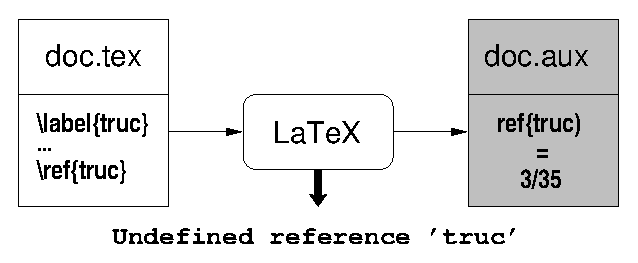
\includegraphics{img/ref1.eps}
    \end{center}
    \caption{使用\dm{.aux}的第一次编译}
    \label{fig:ref1}
  \end{figure}

  因此,此次编译时,会\LaTeX 发送警告,指出标记\dm{truc}未定义。
  \item 我们会进行第二次编译,这次编译会使用辅助文件的内容(如图\ref{fig:ref2}所示)。
  
  \begin{figure}[ht]
    \begin{center}
      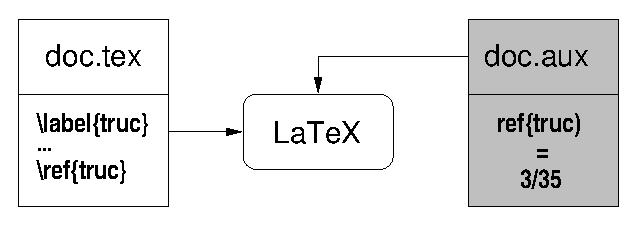
\includegraphics{img/ref2.eps}
    \end{center}
    \caption{使用\dm{.aux}的第二次编译}
    \label{fig:ref2}
  \end{figure}
\end{enumerate}

在以下情况中的引用定义是不正确的。

\begin{enumerate}
  \item 你插入了一个新的标记,并且在插入标记后第一次编译(引用\emph{未被定义})。此时,对于新插入的标记,会得到如下形式的消息:
  
  \begin{dmd}
  Reference 'vlunch' on page 2 undefined on input line 17.
  \end{dmd}

  \item 你在文档中引入的变化无疑会改变页码或对象(图片、方程等)的位置,因此引用会被\emph{错误定义}。在编译结束时,你会看到如下警告:
  
  \begin{dmd}
  Label(s) may have changed.\\
  Rerun to get cross-references right.
  \end{dmd}

  \item 你引用了一个不存在的标记。在这种情况下,再编译八百次也无济于事。
\end{enumerate}

\subsection{与目录的交互}

对于目录,你会发现,其原理与引用是类似的。在文档中插入指令\verb|\tableofcontents|意味着目录将会分两步创建,具体如下。

\begin{enumerate}
  \item 第一轮遍历会收集文档中与\emph{表题}相关的信息,并将其存入文件\codereplace{文件名}\dm{.toc}中(如图\ref{fig:toc1}所示)。
  
  \begin{figure}[ht]
    \begin{center}
      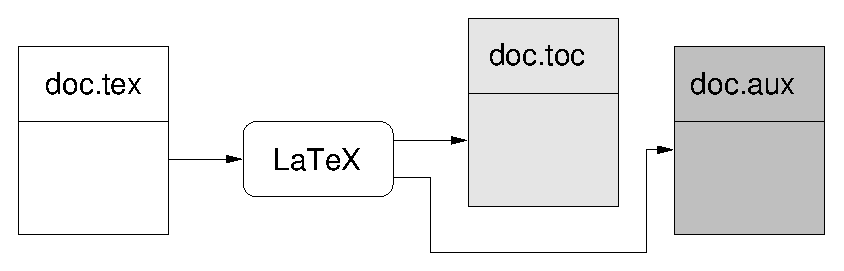
\includegraphics{img/toc1.eps}
    \end{center}
    \caption{使用\dm{.toc}的第一次编译}
    \label{fig:toc1}
  \end{figure}

  \item 第二轮遍历会使最终的文档中包含\codereplace{文件名}\dm{.toc},因此,目录也会被包含(如图\ref{fig:toc2}所示)。
  
  \begin{figure}[ht]
    \begin{center}
      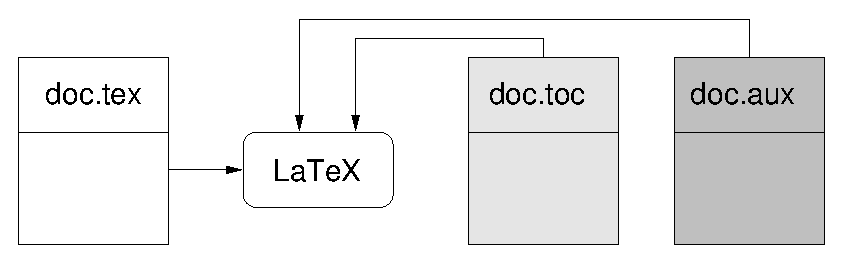
\includegraphics{img/toc2.eps}
    \end{center}
    \caption{使用\dm{.toc}的第二次编译}
    \label{fig:toc2}
  \end{figure}

\end{enumerate}

你可能会遇到这种情况:在写草稿时,文档已经包含了目录指令(\verb|tableofcontents|),而你又添加了新的章节指令。在这种情况下,新的章节只有经过\textbf{两次}编译后才会显示在目录中。

\subsection{一些建议}

要养成为每个文档生成目录的习惯。实际上,\LaTeX 会围绕你的\dm{.tex}文件生成多个文件\jz{
  这还没有涉及参考文献、索引、术语目录等。
}。另外,在起草文档时,不必过于关心目录是否时刻更新——它早晚会更新的!实际上,只有在\textbf{印刷}之前才有必要去确认所有的引用都是正确的。

最后,就像我们在不再能确定目标文件时会时不时运行一下\dm{make clean}指令一样,在看起来一切都运行不正常时,删掉辅助文件\celan{\S B.2}并重新编译是个好习惯。

\section{断字的处理}

\LaTeX 依靠\TeX 对特定的语言来实现不同的断字效果。这种算法在\TeX Book的附录H中有描述,也体现出\TeX 最成功的一面。通过检查文档打断段落的方式,可以识别出文档是不是由\LaTeX 生成的,因为其他很多软件都喜欢以在单词间添加更多空间的方式来处理此类问题。然而,也会有一些\LaTeX 无法正确断字的情况。在这种情况下,\LaTeX 会以以下两种“吓人的”信息之一为你给出警告:

\begin{dmd}
Underfull \backslash hbox (badness 1810) detected at line 33
\end{dmd}

或

\begin{dmd}
Overfull \backslash hbox (14.24376pt too wide) detected at line 41
\end{dmd}

\TeX 在很底层用你的文档生成一系列\emph{字盒}。每个字符都装入合适的字盒,字盒组合成词,再以类似的方式组合成行、成段,然后成页面。

这里以一种简单的方式总结和介绍原理。我们可以简单地理解为,\TeX 在水平模式下操纵\verb|\hbox|来组合单词,在竖直模式下操纵\verb|\vbox|来生成页面。此外,组合这些字盒时,\TeX 如果觉得结果不太美观,就会用以上述两种信息警告你。信息的含义如下。

\begin{itemize}
  \item \verb|Underfull \hbox|表示字盒组合得有些稀疏。通过显示badness的值,\TeX 会告诉你它认为当前行“有多丑”。如果一行文字排列得很完美,该值为0。在最差的情况下,该值为10000.
  \item \verb|Overfull \hbox|表示字盒有些太挤了。\TeX 可以以\dm{pt}为单位显示文字越界深入边缘的长度。
\end{itemize}

如果一个页面过于稀疏,\LaTeX 会以\verb|\vbox|代替\verb|\hbox|显示类似的消息。表\ref{tab:2.4}展示了同一句话的不同疏密程度\yz{
  表中的例句出自法国古典主义戏剧大师高乃依(Pierre Corneille)的戏剧《熙德》(\textit{Le Cid}),意为“哦,愤怒!哦,绝望!哦,宿敌!”。
}排列效果。

\newcommand{\phrase}[1]{\noindent\makebox[\width +
#1][s]{%
  Ô rage ! ô désespoir ! ô vieillesse ennemie !}\par}
\begin{table}[ht] 
\begin{center}
  % \addtolength{\extrarowheight}{4pt} 
  \begin{tabular}{|l|c|}
    \hline
    效果 & 评价 \\
    \hline
    % \typeout{UNDERFULL HBOX AUTORISE}%
    \phrase{1.0cm}  & 稀疏\\
    \phrase{0.75cm} & 稀疏\\
    \phrase{0.45cm} & 稀疏\\
    \hline
    % \typeout{UNDERFULL HBOX AUTORISE}%
    \phrase{0cm}    & 理想 \\ 
    \hline
    \phrase{-0.1cm} & 过密\\
    \phrase{-0.2cm} & 过密\\
    \phrase{-0.25cm} & 过密\\
    \hline
  \end{tabular}
  \caption{横向的不同疏密排列}
  \label{tab:2.4}
\end{center} 
\end{table}

\begin{ii}
  \makebox[\width+2pt][s]{可以在文档选项中启用\dm{draft},来使在出现\dm{Overfull \backslash hbox}问题的位置的侧栏显示一个黑色的\char"258C}
  方块,就像本段的侧栏一样。这个选项可以帮助快速定位导致问题的行。
\end{ii}

\subsection{控制断字}

对于以下情况,\LaTeX 的断字处理可能遇到困难。

\begin{itemize}
  \item 它不能识别需要打断的词——这是个极端情况。
  \item 不能打断的对象占据了需要打断的位置,例如\verb+\verb|...|+或方程类型的对象。
\end{itemize}

这里提供以下几个控制断字的方法。

\begin{exclamation}
如果以下方法都不能使你满意(如果你的句子中包含太多\TeX 不能打断的对象,就会产生这种情况),就只能想办法更换表达方式来规避问题了。
\end{exclamation}

\subsubsection{引导断字}

我们可以通过在必要的位置插入指令\verb|\-|来指出可以断字的位置,从而帮助\LaTeX 实现断字。例如,如果\LaTeX 不能成功地打断“nonmaiçavapamieu”\yz{
  作者的生造词,形似句子“Non, mais ça ne va pas mieux.”,意为“不,没有变得更好”。
}一词,我们可以输入:

\begin{dmd}
\verb|non\-mai\-ça\-va\-pa\-mieu|
\end{dmd}

如果这个词频繁出现,为了避免反复像上面这样给出指示,可以在文前部分输入指令\linebreak \verb|\hyphenation|:

\begin{dmd}
\verb|\hyphenation{non-mai-ça-va-pa-mieu}|
\end{dmd}

这样就可以告诉\LaTeX 这个生词的断字方式。

\subsubsection{强制断字}

通过输入指令\verb|\linebreak[|\codereplace{数字}\verb|]|,我们可以强制断字,但这样做可能带来灾难性的后果——如果你明白我的意思。参数\codereplace{数字}可以调节指令\verb|\linebreak|。你可以“腼腆”地给出指示——\verb|\linebreak[0]|,或是给出不容置疑的命令——\verb|\linebreak[4]|。

指令\verb|\pagebreak[|\codereplace{数字}\verb|]|可以打断页面。另一方面,还有两个指令可以用来换页:

\begin{itemize}
  \item \verb|\clearpage| 完成当前页面,换页另起。
  \item \verb|\cleardoublepage| 完成当前页面,并在双面模式下从奇数页另起。
\end{itemize}

这两条指令会强制\LaTeX 在布局过程中插入所有浮动的图像。%TODO 所以这句是在说啥???

\begin{ii}
另外一种对某些情况很实用的手动介入方式是将当前页面纵向长度加长,需要调用如下指令:

\begin{dmd}
  \backslash enlargethispage
\end{dmd}

指令需要给出尺寸,且其后需要插入一个空行:

\begin{tabbing}
  \verb|\enlargethispage{10cm}   | \= \leftarrow 针对过短的页面 \\
  ~\\
  \verb|[……一段过长的文字……]|\\
  \verb|\clearpage| \> \leftarrow 明确延长10 cm的页面的结尾
\end{tabbing}
\end{ii}

\subsubsection{防止断字}

有三种方式可以强制\LaTeX 不打断文本。

\begin{enumerate}
  \item 通过\verb|~|插入不可打断的空格。
  \item 通过\verb|\mbox{|\codereplace{单词}\verb|}|将词放入一个字盒中\jz{
    这是因为\TeX \textbf{永远不会}打断字盒。
  }。
  \item 对于防止换行使用指令\verb|\nolinebreak|:
  
  \begin{dmd}
  \backslash nolinebreak[\codereplace{数字}]
  \end{dmd}

  同样,为了防止换页,可以使用如下指令:

  \begin{dmd}
    \backslash nopagebreak[\codereplace{数字}]
  \end{dmd}

  其中\codereplace{数字}与\verb|\linebreak|或\verb|\pagebreak|中的作用一致。

\end{enumerate}

\section{小结}

本章介绍了\LaTeX 的标准功能。你如果专心地阅读至此,应该已经可以创建任何类型的简单文档了(目前还不能处理带有公式和图表的文档)。即使你还不能自由地定制你的文档,你的文档的排版质量也会足够好,不需要你提出很多形而上学的问题,如多大的页边距才“理想”、标题和文字间留出多少空白才“合适”……实际上,\LaTeX 中的默认特性已经足够满足全世界范围内有关印刷的大部分实用性规则。

\end{verbatim}
\verb+\backmatter +\textsl{\% 文档末尾的索引内容}
\begin{verbatim}
\bibliographstyle{plain} 
\bibliography{machin,bidule,truc}
\end{document}\end{verbatim}
\end{dmd}

其中的指令\verb|\include|的作用在于,它们减少了你需要同时处理的章节数量,却依然保证了文档的完整性。为此,我们可以在文前部分使用指令\verb|\includeonly|:

\begin{dmd}
\verb|\includeonly{preface,savoir}|
\end{dmd}

使用该指令,可以仅编译前言部分(作为文件\dm{preface.tex}的内容)和文档\dm{savoir.tex}中的章节。

\begin{exclamation}
每条指令\verb|\include|都具有换页的效果,并且似乎没有规避该指令换页的方法。因此,你应该了解,\verb|\include|应当配合能够换页的章节指令(如\verb|\chapter|)使用。若要在插入其他文件时不换页,则应使用指令\verb|\input|,否则这种主文件机制就不会为你带来好处。
\end{exclamation}

最后需要注意到,\verb|\frontmatter|、\verb|\mainmatter|、\verb|\backmatter|这三条指令不是必需的。它们的作用是自动将页码改为罗马数字,常常用于介绍性质的文前页或其他短小部分(然而,它们只在文件类型\dm{book}中可用)。
\chapter{法文文档}

\begin{quote}
    那人说,你所赐给我,与我同居的女人,她把那树上的果子给我,我就吃了。
    
    \hfill《圣经·创世纪》3:12
\end{quote}

了解法文文档要遵循的规则总是好的。严格说来,这些规则并不是无法逃避的准则,而更像是一些使用上的规矩。为了让文档容易可读、避免读者被打断,\emph{建议遵循}这些规则。这些使用上的建议总体上可以让文档看起来更严肃,甚至更专业。有很多关于法文排版的作品,这里给出来自国家印刷局(imprimerie nationale)的汇编材料[7],以及伊夫·佩伊卢梭(Yves Peyrousseaux)的手册[13]。

本章包含一些总结了有关\LaTeX 为实现法文变音符号而使用的字体编码方法的信息,介绍了关于排版的一些规则和用于简化法文输入过程的包\textsf{babel}。本章的末尾介绍了文档类型\dm{letter},其是为信件和传真而设计的。

\section{带有变音符号的字母的问题}

在若干年前,\TeX 的构思阶段完成的时候,其使用的字体不包含带有变音符号的字符。每个字形以7个二进制位区分,这样一共有128个字符可被编码。由于这种方法起源于美国,这128个字符中显然不包括法文中使用的带有变音符号的字符。正因如此,在很长一段时间内,那些优秀的讲法语母语的\TeX 和\LaTeX 用户不得不以一种窘迫方式去录入带有难以输入的字符的法文文档(document en \verb+fran\c{c}ais+ avec des \verb+caract{\`e}res+ assez \verb+p{\'e}nibles+ \verb+{\`a}+ taper)\yz{
    即document en français avec des caractères assez pénibles à taper。原书此处以源代码的方式展示部分单词,以展现其烦琐程度。%原书依然错误渲染了上引号和下引号
}。

今天,这些不悦不再成为人们的糟糕记忆。1990年起,一种容纳了多种语言中带变音符号的字符的字体编码被采用,称为\emph{Cork encoding}或\emph{T1编码(codage T1)}。当然,这种\TeX 编码本身和目前的字符编码标准间存在一定的联系。一些\LaTeX 包就包含了从字符编码(如iso-latin1)到字体编码(如T1编码)的“翻译”操作。

\begin{exclamation}
    于20实际90年代末出现的标准是ISO8859,带有针对称为\emph{latin1}的欧洲语言的编码方案扩展。这也是今天最常用的编码方案。然而,近年来,通用的字符表格\emph{统一码(Unicode)}及其编码\dm{UTF-8}标准得到了大多数系统的良好支持。不幸的是,\LaTeX 引擎最初并没有考虑处理含以多个字节存储的带有变音符号的字符的文档的情况\jz{这正是\dm{UTF-8}面临的情况。}。因此,有多种新型引擎见于公众,如pdftex、xe\TeX 、lua\TeX ,但它们暂时都没有被社区承认为标准。因此,编译以\dm{UTF-8}编码的文件时,需要在这些引擎中自行选用。本书创作时,选用了编码ISO88559和引擎pdftex。
\end{exclamation}

\section{使用\LaTeX 以法文创作}

有两个\LaTeX 包可以将文档“法国化”:\textsf{french}和\textsf{babel}。我们凭借带有绝对偏见的理由选用了后者,使用以下方法激活了包\textsf{babel}:

\begin{dmd}
\verb|\usepackage[francais]{babel}|
\end{dmd}

这条指令出现在文前部分,它使得五个功能运转起来,具体如下。

\begin{description}
    \item[断字] \textsf{babel}在处理段落中的断字时,会考虑法文的使用习惯\jz{
        英文单词和法文单词需要依据不同的规则打断。
    },尤其是会特殊考虑带有变音符号的法文单词。
    \item[排版] 应用法文的排版规则,特别是在面对涉及引号和其他标点符号的情况时。
    \item[版式] 主要涉及为章节标题后的首段文字重新引入首行缩进\jz{在英文排版时不需引入。},为列表替换符号、调整空白等。
    \item[翻译] 将敏感词翻译为法文,如“章”(chapitre)、“目录”(table des matières)等。
    \item[宏] 包\textsf{babel}中提供了一组可用的宏,用于插入一些法文中日常使用的结构,如no、1er、2o、37°C等。
\end{description}

\section{包\textsf{babel}和排版}

与法文排版相关的“规则”集合远远超出了本章的框架。幸运的是,包\textsf{babel}从实践的角度,允许我们在不了解这些规则的情况下去使用它们。我们只需简单地遵守\LaTeX 文档的几条\emph{输入}规则,就能使编译结果遵循那些最常用的排版规则。举例来说,\textsf{babel}会自动在分号前插入一个无法打断的四分之一全空格\yz{全空格(cadratin)指当前字体下字符M的宽度。}。对于法文排版,这是十分常见的做法。

\begin{ii}
如果你不想自动插入此类空格,可以调用指令\verb|\NoAutoSpaceBeforeFDP|。这样一来,你就可以全权决定是否在标点符号前插入空格。
\end{ii}

\subsection{标点符号}

关于标点符号,需要你了解的规则可以总结为以下两点。

\begin{enumerate}
    \item \emph{双}标点——即; : ! ? « »——的前后都应该添加空格。
    \item \emph{单}标点——即. , ( )——的后面应当插入空格,而前面不需要\yz{此处显然是原书纰漏了,左圆括弧的空格应当加在括弧外,即前面。}。
\end{enumerate}

以遵循上述规则的方式输入文档,\textsf{babel}就可以在标点符号前后自动插入空格。对于这个话题,有个有趣的知识点——问号和句号前的空格会更窄一些:

\begin{codelist}[7.1]{
    fouilla\,! et\enspace\,fouilla !
}\begin{verbatim}
fouilla ! et \selectlanguage{english}
fouilla !\selectlanguage{french}
\end{verbatim}
\end{codelist}

\subsection{L-a, e dans l'a, t-i, t-i, a !}

我改编了塞尔日·甘斯堡(Serge Gainsbourg)的歌词作为本小节的标题\yz{
    原歌词为“Elaeudanla teïtéïa”,出自歌曲\emph{Elaeudanla téitéia}。该句歌词描述了拼读Lætitia一词时的发音,其中将æ读作“a, e dans l'a”,即拆读为“a”和“那a中的e”。Lætitia为人名。作者以更贴近Lætitia一词的形式重新拼写该发音作为本小节标题。
},来借此介绍法文中的两个“美丽”的合字:æ和œ。为了输入这两个合字,我们可以选择输入\verb|\ae|和\verb+\oe+(对于大写,则使用\verb|\AE|和\verb+\OE+):

\begin{codelist}[7.2]{
    拉蒂希娅(L\ae titia)去了圣心教堂(Sacré-C\oe ur)。
}\begin{verbatim}
拉蒂希娅(L\ae titia)去了圣心教堂(Sacré-C\oe ur)。
\end{verbatim}
\end{codelist}

如果你的键盘允许,也可以直接输入æ。作为参考,在Linux系统上使用组合键\ovalbox{Alt Gr}+\ovalbox{A}可以输入名副其实地得到这种“a中的e”。出于历史原因,“o中的e”不在范式iso-latin1中,我的键盘不支持直接输入合字æ。

\subsection{包\textsf{babel}中的工具}

在排版时,“是否被排正确”这个问题对于大量细枝末节的内容是很难界定的,例如我想到的以下这些词的缩写:先生、女士、第一、第二、第一,等等。幸运的是,包\textsf{babel}在一定程度上解决了我们的问题。

\begin{center}
    \begin{tabular}{|l|l|}
        \hline
        \verb|1\ier| & 1er\\
        \verb|3\ieme| & 3e\\
        \verb|37\degres{} C| & 37° C\\
        \verb|\primo, \secundo, \tertio, \quarto| & 1o , 2o , 3o , 4o\\
        \verb|\no 4| & no\,4\\
        \verb|\No 4| & No\,4\\
        \hline
    \end{tabular}
\end{center}

\subsubsection{首字下沉}

\lettrine[lines=2]{在}{一些}文档中,我们可以看到\emph{首字下沉(lettrine)}的效果,正如本段所示。包\textsf{lettrine}和贝尔纳·高乐(Bernard Gaulle)的包\textsf{french}定义了此类指令。在本书第II部分,我们会向你介绍一个生成此类指令的\LaTeX 源代码示例。%TODOx2

\subsubsection{摘目}

在法文文档中,我们通常将目录插在文档末尾,而将摘目(sommaire)——目录的摘要——插在文档开头。包\textsf{french}中提供了指令\verb|\sommaire|。正如其名,该指令可以生成文档的摘目。再一次地,我们会在本书第II部分向你介绍生成此类摘目的方法。

\subsection{工具推荐}

包\textsf{babel}的接下来这些推荐使用的功能没有详细说明。它们都是些你可以在排版书籍中可以找到的建议。

\begin{itemize}
    \item 如果你的键盘支持,法文的引号可以直接使用“«”和“»”输入;如果不支持,可以借助小于号和大于号输入:\dm{<<}和\dm{>>}。此外,还可以借助\verb|\og|和\verb|fg|输入:
    
    \begin{codelist}[7.3]{
        Qu'on devra dans ce cas saisir « ainsi ».
    }\begin{verbatim}
Qu'on devra dans ce cas saisir
\og ainsi\fg{}.
    \end{verbatim}
    \end{codelist}

    \item “英文化”的引号可以使用单引号和反引号生成:\verb|``|和\verb|''|。无论如何,直接使用“\verb|"|”作为引号都是不推荐的。
    
    \item 拉丁短语\emph{理论上(a priori)}应以意大利体输入。
    
    \item 有以下缩写规则\jz{
        其中,Monsieur不应缩写为“Mr.”——这是英文\emph{mister}的缩写。
    }:

    \begin{center}
        \begin{tabular}{|l|l|l|}
            \hline
            \emph{et cætera} & 缩写为\quad \verb|etc.| & etc.而不是“etc...” \\
            Monsieur & 缩写为\quad \verb|M.| & M. Machin \\
            Messieurs & 缩写为\quad \verb|MM.| & MM. Machin et Bidule\\
            Madame & 缩写为\quad \verb|M\up{me}| & M$^{\rm me}$ Machin\\
            Mademoiselle & 缩写为\quad \verb|M\up{lle}| & M$^{\rm lle}$ Machin\\
            kilomètre(s) & 缩写为\quad \verb|km| & 25 km(不加s)\\
            kilogramme(s) & 缩写为\quad \verb|kg| & 25 kg\\
            \hline
        \end{tabular}
    \end{center}

    \item 法文中,整数与小数间的分割符为\emph{逗号},而英文中为圆点。因此我们“应当”这样写:123,54。
    
    \item 每逢千位或千分位\yz{即从小数分割符向两侧每三位。},要插入四分之一全空格:
    \begin{codelist}[7.4]{
        12\,345\,678,234\,34
    }\begin{verbatim}
\nombre{12345678,23434}
    \end{verbatim}
    \end{codelist}

    \item 可以将专有名词写成小型大写字母的形式,比如John \textsc{Coltrane}。这里使用的方式是\linebreak\verb|\textsc{Coltrane}|,但包\textsf{babel}中包含了宏\verb|\bsc|,可以忽略大小写。也就是说,\verb|\bsc{COLTRANE}|、\linebreak\verb|\bsc{Coltrane}|和\verb|\bsc{coltrane}|都可以生成预期的结果。
    
    \item 首字母缩合词应采用大写,并且不加圆点,如RATP\yz{全称为Régie autonome des transports parisiens,即巴黎独立运输公司。}、SNCF\yz{全称为Société nationale des chemins de fer français,即法国国家铁路公司。}、ENISE\yz{即国立圣-埃蒂安工程师学院。}。如果首字母缩合词“可以直接读出来”,则也可以使用小写字母,如Assedic\yz{全称为Association pour l'Emploi dans l'Industrie et le Commerce,即工商业就业协会。}、Inserm\yz{全称为Institut national de la santé et de la recherche médicale,即全国保健和医学研究所。}等。
\end{itemize}

\subsection{欧元符号}

欧元符号可以借助包\textsf{textcomp}中的指令\verb|\texteuro|生成。因此,我们可以得到€。如果使用非衬线字体,则有\textsf{€}。另一种输入方式是借助包\textsf{eurosym},支持如下指令。

\begin{itemize}
    \item \verb|\euro{}|:€。
    \item \verb|\euro{35}|:35€。
\end{itemize}

\subsection{说到大写……}

除了耳熟能详的应当或不应当使用大写的情况(句首应大写,括号内首字母不应大写,冒号后取决于具体内容,等等),关于大写(majuscule;对于印刷工人,会称作capitale),有以下三个要点。

首先,\textbf{大写字母也应带有变音符号}(我没生气,我在解释)。伊夫·佩伊卢梭的手册中有关于此的说法:大写字母的变音符号自16世纪以来就一直存在,但随着盎格鲁-撒克逊人带来的打字机和印刷排版技术而消失了。我们同样可以在各种优秀的排版图书中找到因没有添加变音符号而导致歧义的例子。

其次,\emph{对于标题},我们只将全句的首字母大写(与此相反,英文中会将每个单词的首字母大写)。最后,需要强调,大写字母如何使用是很微妙的,大写字母的使用与否会带来微妙的差别。这里展示了一些示例,可以让你领会这些“规则”:

\begin{itemize}
    \item maître de conférences(也就是不用大写);
    \item l'université Jean Monnet(université一词不大写);
    \item 当谈论作为独立实体的结构时,写成l'Université;
    \item le ministre de l'Intérieur;
    \item l'académie de Lyon;
    \item l'Assemblée nationale、le Sénat,因为它们是独立机构;
    \item les Espagnols(指人)、le français(指语言)。
\end{itemize}

我不反对雅克·安德烈(Jacques André)的观点:

\begin{quote}
    ……我们在活动报告中找到了这样一句典型的话:
    
    \begin{quote}
        Jean Transent, Maître de Conférence en Analyse de Données à l'Université de Nancy (Bien connue de la Communauté Scientifique Internationale) a donné, lors du séminaire de Biologie Informatique de Mardi 23 Juin, une conférence sur les Applications de l'Intelligence Artificielle à l'emploi de la Télévision Haute Dé- finition en Robotique Avancée.
    \end{quote}

    这句话中共有23个大写字母,但按理来说,应当只有3个,分别用于Jean、Transent和Nancy。是的,没错……
    
    \hfill 雅克·安德烈[2]
\end{quote}

我也不反对伊夫·佩伊卢梭的观点:

\begin{quote}
    用于体现尊严、权力、等级或职能的名头\textbf{是普通的称谓}:
    \begin{itemize}
        \item ……
        \item 总理事会主席(le président du conseil général),等等。\\\textsf{这是个普通的称谓,就像总理事会保安或总理事会保洁一样。}
    \end{itemize}

    \hfill 伊夫·佩伊卢梭[13]
\end{quote}

\section{信件和传真}

\LaTeX 的核心包含了用于写信的文档类型。然而,这个类型不够灵活,也没有很好地兼容\linebreak 法文\jz{
    1999年2月9日基于文档类型\dm{class} 1.2z版本的个人评价。
}。对于法文信件,我们建议你使用来自日内瓦天文台的德尼·梅吉翁(Denis Megévand)开发的文档类型\dm{lettre}。该类型和其文档可以在\wz{obsftp.unige.ch/pub/tex/macros/lettre}找到,也可以在发行版Debian Sarge中的包\dm{tetex-frogg}中找到。

\subsection{可用指令}

以下是我们在信件类型中可以定义的几个实体。

\begin{description}
    \item[寄件人地址] 使用指令\verb|\address|。
    \item[出发地] 使用\verb|\lieu|可以在页面右上方书写下我们的信件来自何地。
    \item[电话和传真] 分别使用指令\verb|\telephone|和\verb|\fax|指明。
    \item[签名] 使用指令\verb|\signature|。
    \item[信件主题] 使用指令\verb|\conc|(指concernant,即“关于”)。
    \item[附件] 使用指令\verb|\encl|(指英文的\emph{enclosed}) 。
\end{description}

\subsection{基于类型\dm{lettre}的文档}

图\ref{fig:7.1}展示了使用类型\dm{lettre}的\LaTeX 文档骨架。指令\verb|\opening|和\verb|\closing|是必需的,分别对应在信件首尾引入礼貌用语的对象。

\begin{figure}[tb]
    \rotatebox{90}{%
      \begin{minipage}{.5\linewidth}
        \begin{footnotesize}
          \VerbatimInput{texs/ossature.tex}
        \end{footnotesize}
      \end{minipage}%
    \setlength{\fboxsep}{-\fboxrule}%
    \quad
    \fbox{\begin{minipage}{.7\linewidth}
        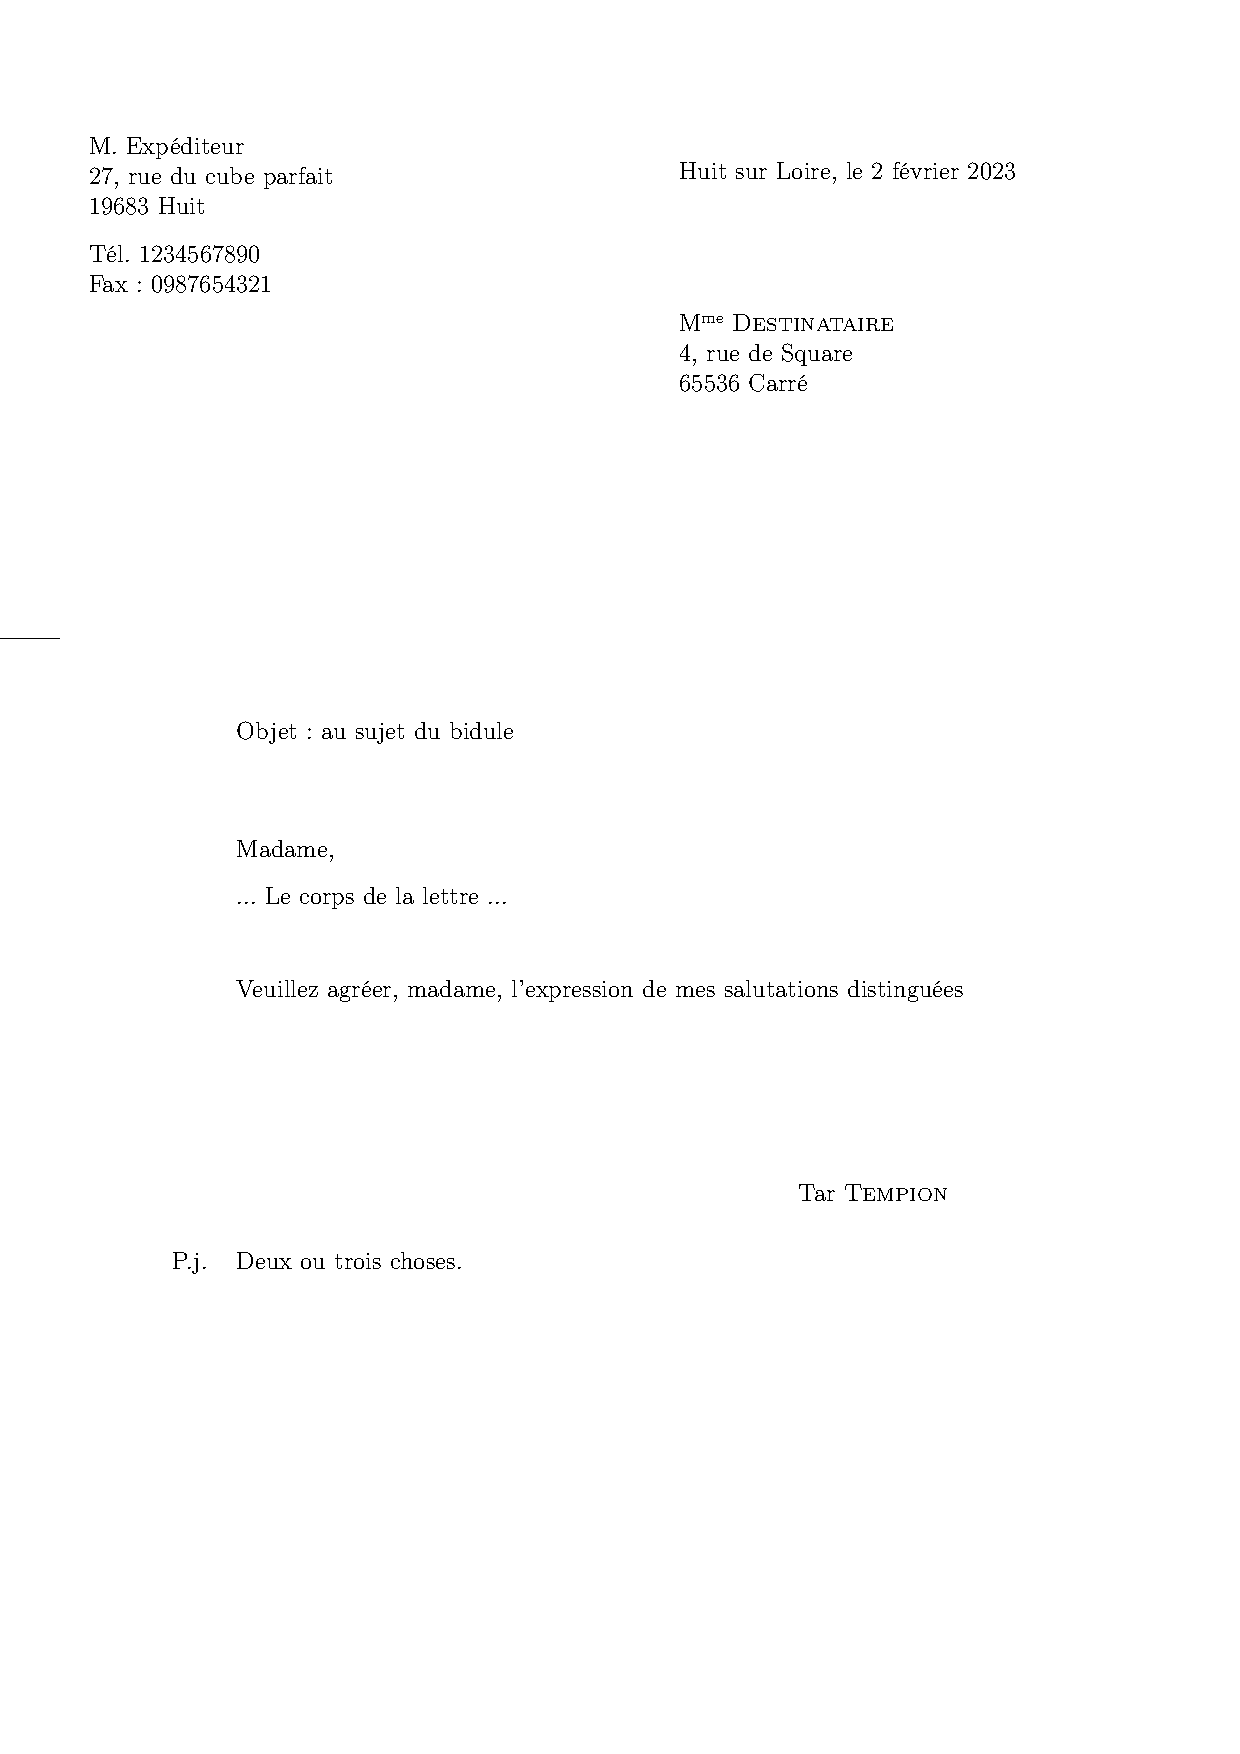
\includegraphics[width=\textwidth]{img/ossature}
      \end{minipage}}}
  \caption{基于类型\dm{lettre}的文档“骨架”}
  \label{fig:7.1}
  \end{figure}

\subsubsection{“协会”文件}

类型\dm{lettre}借助文件\dm{default.ins}交付。该文件默认定义了日内瓦天文台的地址。你使用的\LaTeX 系统管理员应当将该文件适配为你的组织。

我们可以定义自己的“协会”文件,并将其包含在信件中。但实际上,当我们想以私人名义寄信时,使用私人通信地址更符合逻辑。因此,我们可以定义名为\dm{moi.ins}的文件,并在其中包含相应信息,例如:

\begin{dmd}
\begin{verbatim}
\address{%
    M. Expéditeur\\
    27, rue du cube parfait\\
    19683 Huit}
\lieu{Huit sur Loire}
\telephone{1234567890}
\fax{0987654321}
\signature{Tar \textsc{Tempion}}
\end{verbatim}
\end{dmd}

此时,只需借助指令\verb|\institut|在文档的文前部分调用它。该指令会寻找带有扩展名\dm{.ins}的文件:

\begin{dmd}
\verb|\institut{moi}|
\end{dmd}

\subsection{传真}

信件类型中,同样包含用于传真的环境,它带有你所在组织的笺头。通用的原则和关键字与信件是相同的,只不过需要使用环境\dm{telefax}而不是环境\dm{letter}。

注意,这里我们仍然可以使用“机构”文件。毕竟,指令\verb|\addpages|可以用于需要在传真中附加已打印文档的情况。例如,你不得不向初始传真发送$n$页,就可以添加指令\verb|\addpages{|\codereplace{$n$}\dm{\}}。图\ref{fig:7.2}展示了创建传真需要的最小文档。



\begin{figure}[tb]
    \rotatebox{90}{%
      \begin{minipage}{.5\linewidth}
        \begin{footnotesize}
          \VerbatimInput{texs/ossature-fax.tex}
        \end{footnotesize}
      \end{minipage}%
    \setlength{\fboxsep}{-\fboxrule}%
    \quad
    \fbox{\begin{minipage}{.7\linewidth}
        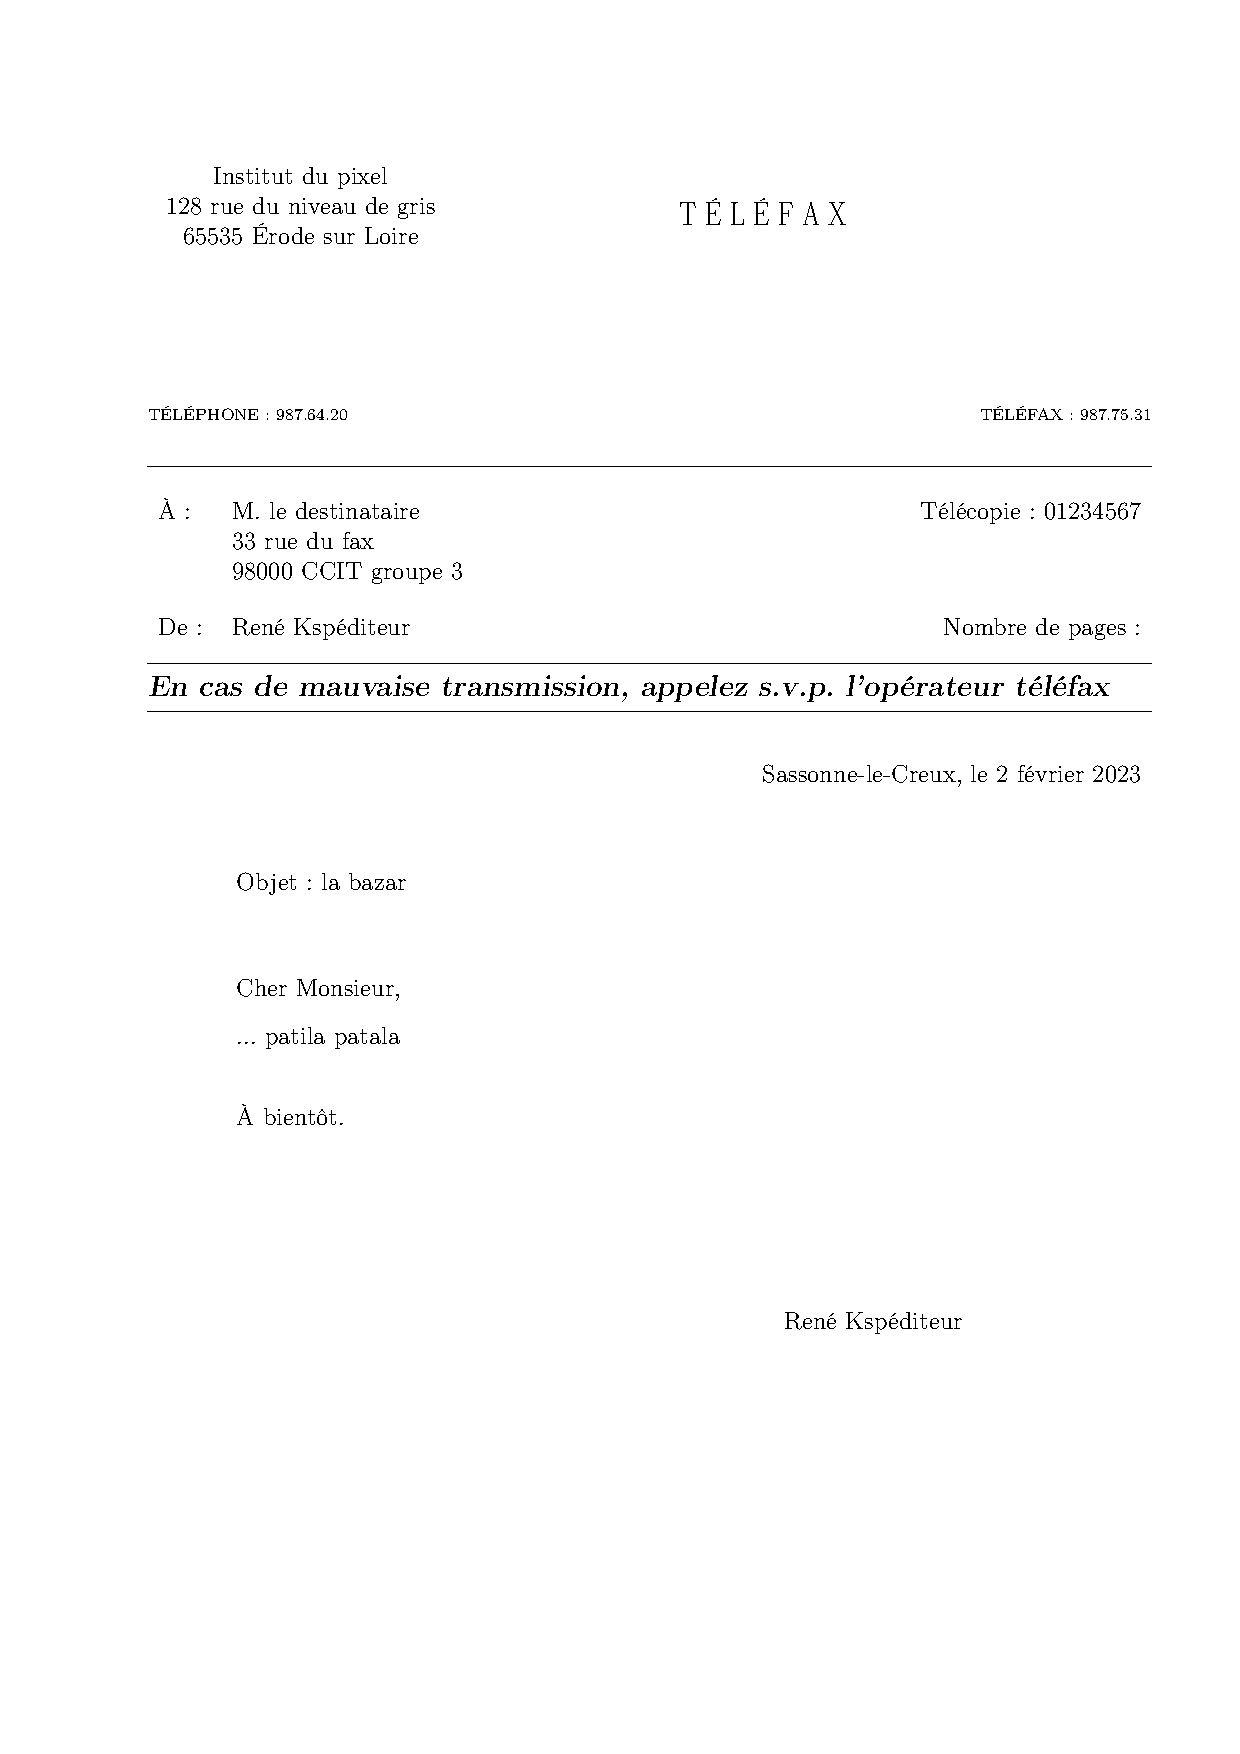
\includegraphics[width=\textwidth]{img/ossature-fax}
      \end{minipage}}}
  \caption{传真文档的“骨架”}
  \label{fig:7.2}
  \end{figure}
\chapter{你的回合!}

\begin{quote}
    不可与男人苟合,像与女人一样,这本是可憎恶的。

    \hfill《圣经·利未记》18:22
\end{quote}

\part{关于《关于\LaTeX 的那些你想知道却从不敢问的问题》的那些你想知道却从不敢问的问题}

\chapter*{简介}

\begin{quote}
    王女阿,你的脚在鞋中何其美好。你的大腿圆润,好像美玉,是巧匠的手做成的。你的肚脐如圆杯,不缺调和的酒。你的腰如一堆麦子,周围有百合花\jz{
        本部分的题记都取自《雅歌》,与章标题毫无关联。
    }。

    \hfill《圣经·雅歌》7:2
\end{quote}

本部分的名为“关于《关于\LaTeX 的那些你想知道却从不敢问的问题》的那些你想知道却从不敢问的问题”,旨在解释此前的各章节是如何生成的,并借此介绍已定义的用于生成你当前看到的这本书的指令和环境。本部分的目标更宏大一些,因为我们希望为有勇气的读者提供用于创建其自己的风格的坚实知识基础……

在遇到读者询问是否可以复用本文档中这样或那样的风格的问题后,我萌生了编写接下来的章节的想法。对于我来说,继续向下编写这项工作有些艰巨,因为我需要介绍的\LaTeX 知识超出了基础知识的范畴,也因此更难解释。最后,同样重要的是,在这里,我自己的巴扎中的剩货通常必须被“合理化”,才能成为可介绍的内容。这可不是件好搞的事。

在这一部分,我想介绍些生成本文档时使用的手段。我的手段不是能获得你当前看到的版式的唯一方法。例如,文档中的一些部分可以借助一些具有类似功能的包来完成,这些包甚至能比这里开发的工具生成更好的效果。

这一部分隐藏的思想是将好奇的读者领到探索\LaTeX 的小路上,并向他们展示:我们可以借助几个工具,将原指令校准到可以严格适用于他们自己的需求的程度。这些小路具有足够的普适性,可以用于按图索骥,也可以针对类似或不同的情况来调整。这里的关键,一方面是发现“\LaTeX ”内部功能的经典之处,另一方面通过创造自己的工具来获得满足感——但针对这件事,我们不宣扬“重新发明”轮子。

我尝试尽可能只介绍\LaTeX 指令。然而,有时也有必要使用一些\TeX 的功能,这里也是一个介绍这些功能的机会。因此,这一部分由三章组成。

\begin{description}
    \item[必要工具] 介绍需要了解的指令,以为接下来的工作做准备。例如,在这里,我们可以找到\LaTeX 发行版中文件结构的踪迹、切换文档弟子的思路,以及关于基于列表创建新环境的详细介绍;
    \item[装饰] 介绍了我们实现的工具,它们用于修改标题、页眉页脚、侧栏以及其他一些细枝末节的风格。
    \item[新玩具] 这里解释了本书的侧面标签、术语字典、示例、摘要、首字下沉、提示框,以及其他一些细碎的内容的创建过程。
\end{description}

\begin{qquestion}
这些章节中给出的一些解释显得有些云里雾里,即使是作者也无法理解。问题的一些解决方案是片面的。然而,对于鄙人来说,一些内容仍然很神秘。在这些情况下,段落中会插入这种“路面不平”(dos d'âne)\yz{
    原作者已经把这个标志替掉了。在源文档中可以找到名为\dm{dosdane.eps}的文件,指的就是这里说的已经被弃用的标志。
}标志。
\end{qquestion}
\chapter{必要工具}

\begin{quote}
    我所爱的,你何其美好。何其可悦,使人欢畅喜乐。你的身量好像棕树。你的两乳如同其上的果子,累累下垂。

    \hfill《圣经·雅歌》7:7
\end{quote}

在本章,我们会介绍创造比第4章中介绍的指令和环境更复杂的指令和环境所需准备的工具。此外,借着本章的介绍,我们旨在说明,此处提到的第4章需要正确消化,才能继续这一部分的阅读。本章也会介绍一些关于字体的机制,以及挖掘\LaTeX 资源的方法。

\section{赫尔克里·波洛}

\subsection{在文件中挖掘信息}

首先,为了让使用\LaTeX 写成的文档带有一些个人特色,需要知道组成你使用的\TeX 或\LaTeX 的发行版的文件的组织方法。鄙人使用了UNIX平台的发行版\TeX Live(\wz{http://www.tug.org/texlive})。在这个发行版中,我们可以在第一时间在以下目录中查阅各种包的文档:

\begin{dmd}
/usr/share/texmf-texlive/doc/latex/
\end{dmd}

这个目录中包含其他子目录,通常每个子目录对应一个包,其中就以DVI或PostScript文件的形式提供了文档。在一些情况下,需要去检查这些包的源代码。在发行版te\TeX 中,这些源代码位于:

\begin{dmd}
/usr/share/texmf-texlive/tex/latex
\end{dmd}

在同样的位置,我们通常可以为每个包找到一个目录,包含文本形式且带有扩展名\dm{sty}的源代码,在必要时也会包含相关文件。最后,为了独立于我们可以包含的包而了解\LaTeX 的默认行为,可以借助以下位置的\LaTeX 源代码:

\begin{dmd}
/usr/share/texmf-texlive/tex/latex/base/latex.ltx
\end{dmd}

对于文档类型\dm{book},还可以借助以下位置的文档类型源代码:

\begin{dmd}
/usr/share/texmf-texlive/tex/latex/base/book.cls
\end{dmd}

\subsection{检查宏}

查找指令定义的一个非常便捷的方法是在交互式会话中求助于\LaTeX 。可以直接在操作系统的命令行终端中执行以下指令:

\dmh{latex}

我的系统是这样冷冰冰地回答的:

\begin{dmd}
\begin{verbatim}
This is e-TeXk, Version 3.14159-2.1 (Web2C 7.4.5)
%&-line parsing enabled.
**
\end{verbatim}
\end{dmd}

在“赤裸裸的\TeX ”呼喊出这个冷峻的提示(\dm{**})的邀请下,我勇敢地回复了\verb|&latex|来要求加载\LaTeX 格式。没有丝毫延迟,就得到了答复:

\begin{dmd}
\begin{verbatim}
**&latex
entering extended mode
LaTeX2e <2001/06/01>
Babel <v3.7h> and hyphenation patterns for american,
french loaded.
*
\end{verbatim}
\end{dmd}

注意,提示中少了一个星号。从现在开始,我们就可以交互式地编写\LaTeX 文档了。从绝对意义商来说,这样做的乐趣不大,但从获取指令的定义和语法上来说,却很有帮助。因此,举例来说,我们可以写下这样的指令:

\begin{dmd}
\verb|*\show|\codereplace{指令}
\end{dmd}

这样可以获取\codereplace{指令}的定义。例如:

\begin{dmd}
\begin{verbatim}
*\show\mbox
> \mbox=\long macro:
\end{verbatim}
\verb|#1->\leavevmode \hbox {#1}.| \quad $\leftarrow$\textsf{此处为定义}\\
\verb+<*> \show\mbox+
\end{dmd}

其中向我们提供了指令\verb|\mbox|的定义。可以注意到,该指令被调用时,将这种调用转化为对\verb|\leavevmode|和\verb|\hbox|的调用。在好奇心的驱使下,我们继续查看指令的定义:

\begin{dmd}
\verb|*\show\hbox|\\
\verb|> \hbox=\hbox.| \quad $\leftarrow$\textsf{这是一个原语}\\
\verb|<*> \show\hbox|
\end{dmd}

可以观察到,\verb|\hbox|不是由其他指令定义而成的。在\TeX 中,这种指令称为原语(primitive)。我们的探索可以继续:

\begin{dmd}
\verb|*\show\leavevmode|\\
\verb|> \leavevmode=macro:|\\
\verb|->\unhbox \voidb@x .|\quad $\leftarrow$\backslash leavevmode\textsf{的定义}\\
\verb|<*> \show\leavevmode|
\end{dmd}

以此类推……

\section{底层工具}

\subsection{百分号图个什么?}

你可能已经注意到,有时\LaTeX 源代码中的行末带有百分号\dm{\%}。基于代码换行时文本间会自动添加空格这样的情况,百分号就有理由出现了。请看如下指令:

\begin{dmd}
\verb|\newcommand{\beurk}{bidule}|
\end{dmd}

为了增强可读性,这条指令可以拆分为多行代码:

\begin{codelist}[9.1]{
\newcommand{\beurk}{
    bidule
}
==(\beurk)==
}\begin{verbatim}
\newcommand{\beurk}{
    bidule
}
==(\beurk)==
\end{verbatim}
\end{codelist}

可以观察到,“bidule”一词的两侧出现了我们不想要的空格。为了避免这种现象,可以使用如下方式改写:


\begin{codelist}[9.2]{
\newcommand{\beurk}{%
    bidule%
}
==(\beurk)==
}\begin{verbatim}
\newcommand{\beurk}{%
    bidule%
}
==(\beurk)==
\end{verbatim}
\end{codelist}

在另一些场景下,空格会为行文带来有害的干预。定义以下环境:

\begin{dmd}
\begin{verbatim}
\newenvironment{hyperimportant}{% 
    \bfseries\itshape}{% 
    \upshape\mdseries}
\end{verbatim}
\end{dmd}

\newenvironment{hyperimportant}{% 
    \bfseries\itshape}{% 
    \upshape\mdseries}

\begin{codelist}[9.3]{
    Il est impératif
\begin{hyperimportant}
  de multiplier les sauvegardes
\end{hyperimportant}
de vos documents personnels
}\begin{verbatim}
Il est impératif
\begin{hyperimportant}
    de multiplier les sauvegardes
\end{hyperimportant}
de vos documents personnels
\end{verbatim}
\end{codelist}

如果仔细观察生成的文本,可以注意到,在粗斜体部分文本“{\bfseries\itshape de ... sauvegardes}”的两侧各有两个空格:

\begin{itemize}
    \item “{\bfseries\itshape de}”前面的两个空格分别由“\dm{impératif}”和begin条目“\verb|\begin{hyperimportant}|”后的换行引入;
    \item “{\bfseries\itshape sauvegardes}”后面的两个空格分别由“\dm{sauvegardes}”和end条目“\verb|\end{hyperimportant}|”后的换行引入。
\end{itemize}

我们可以删除换行,来证明这种观点:

\begin{codelist}[9.4]{
Il est impératif\begin{hyperimportant} de
multiplier  les
sauvegardes\end{hyperimportant} de vos
documents personnels
}\begin{verbatim}
Il est impératif\begin{hyperimportant} de
multiplier  les
sauvegardes\end{hyperimportant} de vos
documents personnels
\end{verbatim}
\end{codelist}

为了防止被这种问题牵扯精力,一般可以求助于两条用于删除双重空格的指令。对于序列之前的双重空格,可以调用指令\verb+\ignorespaces+来消除它;对于序列之后的,可以调用\verb|\unskip|。

\subsubsection{指令\dm{\backslash ignorespaces}}

该指令可以展开后续的指令,并忽略后面的所有空格:

\begin{codelist}[9.5]{
\newcommand{\truc}{ }
\newcommand{\bidule}{ }

a\truc\bidule b\par
a\ignorespaces\truc\bidule b
}\begin{verbatim}
\newcommand{\truc}{ }
\newcommand{\bidule}{ }

a\truc\bidule b\par
a\ignorespaces\truc\bidule b
\end{verbatim}
\end{codelist}

以上示例中,指令\verb|\truc|和\verb|\bidule|的唯一作用都是在被调用时生成空格。例如,以下指令会生成“\verb*|a { }b|”:

\begin{dmd}
\verb|a\truc\bidule b|
\end{dmd}

也就是说,字母a和b之间由两个空格隔开。调用指令\verb|\ignorespaces|——正如其名——可以忽略指令\verb|\truc|和\verb|\bidule|产生的空格。因此,对于前面的示例,可以使用以下指令:

\begin{dmd}
\begin{verbatim}
\newenvironment{hyperimportant}{% 
    \bfseries\itshape\ignorespaces}{\upshape\mdseries}
\end{verbatim}
\end{dmd}

这样就能删除一个空格:

\renewenvironment{hyperimportant}{% 
    \bfseries\itshape\ignorespaces}{\upshape\mdseries}

\begin{codelist}[9.6]{
    Il est impératif
\begin{hyperimportant}
    de multiplier les sauvegardes
\end{hyperimportant}
de vos documents personnels.
}\begin{verbatim}
Il est impératif
\begin{hyperimportant}
    de multiplier les sauvegardes
\end{hyperimportant}
de vos documents personnels.
\end{verbatim}
\end{codelist}

\subsubsection{指令\dm{\backslash unskip}}

如果细心一些,我们可以发现,“{\bfseries\itshape sauvegardes}”和“de”之间仍然有两个空格抵住了我们的攻击。这就到了\TeX 的原语\verb|\unskip|的用武之地:它可以删除后一个被插入的空格:

\begin{codelist}[9.7]{
    \newcommand{\truc}{ }
\newcommand{\bidule}{ }
a\truc\bidule b\par
a\truc\bidule\unskip b
}\begin{verbatim}
\newcommand{\truc}{ }
\newcommand{\bidule}{ }
a\truc\bidule b\par
a\truc\bidule\unskip b
\end{verbatim}
\end{codelist}

最后,我们环境的“正确”定义如下:

\begin{dmd}
\begin{verbatim}
\newenvironment{hyperimportant}{% 
    \bfseries\itshape\ignorespaces}{\unskip\upshape\mdseries}
\end{verbatim}
\end{dmd}

这样,就可以删除所有我们不希望插入的空格:

\renewenvironment{hyperimportant}{% 
    \bfseries\itshape\ignorespaces}{\unskip\upshape\mdseries}

\begin{codelist}[9.8]{
Il est impératif
\begin{hyperimportant}
  de multiplier les sauvegardes
\end{hyperimportant}
de vos documents personnels.
}\begin{verbatim}
Il est impératif
\begin{hyperimportant}
  de multiplier les sauvegardes
\end{hyperimportant}
de vos documents personnels.
\end{verbatim}
\end{codelist}

\subsection{字符\dm{@}}

在开始探索包的源代码时,你会发现,有很大一部分的指令名称定义中都带有字符\dm{@}。然而,在\dm{.tex}文档中,不允许执行名称带有该字符的指令。这样可以保护或限制包指令的能力范围。例如,在包\textsf{changebar}中定义了指令\verb+\cb@defpoint+,它不能被包的使用者调用。若要重定义该内部指令,需要做出以下小操作:

\begin{dmd}
\begin{verbatim}
\makeatletter
% 我们可以在这里胡说八道
\renewcommand{\@ttention}{oulala...}
\makeatother
% 但在这里就不行了
\end{verbatim}
\end{dmd}

这里举例的指令\verb+\@ttention+只有在字符\dm{@}被当作字母的情况下才能被操作。这正是\verb+\makeatletter+的作用:将字符\dm{@}转化为字母,就像其他字母一样。而指令\verb+\makeatother+可以重新赋予该字符区别于其他字母的特殊性。

\begin{exclamation}
这种操作在使用指令\verb+\usepackage+包含的风格文件中不是必需的。对于这些文件,字符\dm{@}可以当作字母使用。
\end{exclamation}

\TeX 得以更改此字符的类别的方法在10.5.1小节会详细解释。

\subsection{\TeX 的\dm{\backslash let}}

有时,修改\LaTeX 内部的指令以在其默认行为中添加功能是很有用的做法。例如,为了修改内部指令\verb+\bidule+\jz{
    好吧,这并不是一条内部指令。它只是作为愚蠢的例子而使用的指令名称……
},可以遵循以下步骤。

\begin{enumerate}
    \item 借助\TeX 的指示\verb+\let+保存该指令:
    
    \begin{dmd}
    \verb|\let\biduleORIG\bidule|
    \end{dmd}

    \item 在初始定义的基础上重新定义指令\verb+\bidule+:
    
    \begin{dmd}
    \begin{verbatim}
\renewcommand{\bidule}{%
    一些新东西\biduleORIG}
    \end{verbatim}
    \end{dmd}

    \item 如果有需要,可以借助如下指令重新回到其原定义:
    
    \begin{dmd}
    \verb+\let\bidule\biduleORIG+
    \end{dmd}
\end{enumerate}

\section{控制结构和测试}

包\textsf{ifthen}引入的结构遵循以下语法:

\begin{dmd}
\verb+\ifthenelse{+\codereplace{布尔表达式}\}\\
\{……若真,\LaTeX 代码……\}\\
\{……若假,\LaTeX 代码……\}
\end{dmd}

以及

\begin{dmd}
\verb+\whiledo{+\codereplace{布尔表达式}\}\\
\{……只要为真时,\LaTeX 代码……\}
\end{dmd}

\codereplace{布尔表达式}可以根据可以由包\textsf{ifthen}中不同指令的上下文构成,具体如下:

\begin{itemize}
    \item 表达式\codereplace{数$_1$}\dm{>}\codereplace{数$_2$}、\codereplace{数$_1$}\dm{<}\codereplace{数$_2$}及\codereplace{数$_1$}\dm{=}\codereplace{数$_2$}都可以用于比较\codereplace{数$_1$}和\codereplace{数$_2$};
    \item \verb+\equal{+\codereplace{$C_1$}\verb+}{+\codereplace{$C_2$}\dm{\}}可以根据字符串\codereplace{$C_1$}是否等于\codereplace{$C_2$}来返回真或假;
    \item \verb+\isodd{+\codereplace{数}\verb+}+在\codereplace{数}是奇数的时候返回真,否则返回假;
    \item \verb+\value{+\codereplace{计数器}\dm{\}}可以以可被布尔条件使用的形式返回\codereplace{计数器}的值;
    \item \verb+\lengthtest{\codereplace{长度检验}+\dm{\}}返回表达式\codereplace{长度检验}的结果,所谓“长度检验”包含操作符\dm{>}、\dm{<}或\dm{=}和作为运算量的\LaTeX 长度。
\end{itemize}

可以注意到,我们可以使用逻辑连接符\verb+\OR+、\verb+\AND+和\verb+\NOT+,它们在布尔表达式中扮演的正是我们所想象的角色。也可以使用操作符\verb+\(+和\verb+\)+来组合表达式。

\subsection{布尔值和相关操作符}

包\textsf{ifthen}为其朝气蓬勃的用户提供了操作布尔值的方式。可以使用指令\verb+\newboolean+声明一个布尔值:

\begin{dmd}
\verb+\newboolean{+\codereplace{布尔值标识}\}
\end{dmd}

这样就定义了一个可以以\codereplace{布尔值标识}唯一指代的布尔值。接下来,可以使用指令\verb+\setboolean+为其赋值\dm{true}或\dm{false}:

\begin{dmd}
\verb|\setboolean{|\codereplace{布尔值标识}\}\{\codereplace{值}\}
\end{dmd}

当然,可以在控制结构\celan{\S 9.3}中使用以此种方式创建的布尔值,例如:

\begin{dmd}
\verb|\ifthenelse{\boolean{|\codereplace{布尔值标识}\}\}\\
\{……\codereplace{布尔值标识}为真时的\LaTeX 代码……\}\\
\{……\codereplace{布尔值标识}为假时的\LaTeX 代码……\}
\end{dmd}

这里提议了解一下前面内容中的\TeX 版本。实际上,我们可以在\LaTeX 包中找到使用\TeX 编写的代码,特别是对结构“若--则--否则”的使用。如下示例使用了\TeX 定义了新的布尔值\yz{
    其中,imprimante couleur意为“彩色打印机”。
}:

\begin{dmd}
\verb|\newif\ifimprimantecouleur|
\end{dmd}

使用如下指令将其置为假:

\begin{dmd}
\verb|\imprimantecouleurfalse|
\end{dmd}

使用如下指令将其置为真:

\begin{dmd}
\verb|\imprimantecouleurtrue|
\end{dmd}

接下来,就可以在\TeX 模式的结构“若--则--否则”中操作这个布尔值:

\begin{dmd}
\backslash ifimprimantecouleur\\
... \textsl{\% 针对彩色打印机的代码}\\
\backslash else\\
... \textsl{\% 针对黑白打印机的代码}
\end{dmd}

\subsection{示例}

我们希望通过编写指令来生成阶乘函数的展开\jz{
    有人整天没什么事情可做……
},使得以下方法可以生成预期效果:

\begin{codelist}[9.9]{
    9的阶乘可以表达为:
    \begin{displaymath}
        9!=9\times 8\times 7\times 6\times 5\times 4\times 3\times 2\times 1
    \end{displaymath}
}\begin{verbatim}
9的阶乘可以表达为:
\begin{displaymath}
    9!=\itfactorielle{9}
\end{displaymath}
\end{verbatim}
\end{codelist}

解决该问题的一种方法是,编写一个指令,其中包含循环\verb|\whiledo|:

\begin{dmd}
    \begin{verbatim}
\verb|\newcommand{\itfactorielle}[1]{%
    \setcounter{cptfact}{#1} % 使用一个计数器来存储变量
    \whiledo{\value{cptfact}>1}{ % 只要变量大于1
    \thecptfact\times % 显示一个乘号
    \addtocounter{cptfact}{-1}} % 计数器递减
1} % 在末尾显示1
    \end{verbatim}
\end{dmd}

当然,需要声明计数器:

\begin{dmd}
\verb+\newcounter{cptfact}+
\end{dmd}

可以注意到,在“只要……”循环中的布尔条件中,我们调用了指令\verb|\value|来比较计数器的值和1。更迂回的办法是,我们可以以递归的方式来实现这个指令:

\begin{dmd}
\begin{verbatim}
\newcommand{\recfactorielle}[1]{ % 递归的方式
\setcounter{cptfact}{#1} % 为计数器赋值
\ifthenelse{#1>1}{ % 如果值大于1
    \thecptfact\times % 显示计数器,并紧跟一个乘号
    \addtocounter{cptfact}{-1} % 计数器递减
    \recfactorielle{\thecptfact}} % 做一次递归调用
{1}} % 否则(即值为1)显示1
\end{verbatim}
\end{dmd}

该指令当然与之前的方法生成相同的结果。注意到,在\verb|\ifthenelse|的条件中,我们将一个数(\dm{\#1})与另一个数(1)作比较。我们也能注意到,\verb|\times|的出现说明了该指令需要在数学模式中执行。如果有需要,我们也可以通过指令\verb|\ensuremath|\celan{\S 4.5.1}来避开这个问题。

在你当前阅读的这个文档中,使用了\verb|\whiledo|\verb|\ifthenelse|来生成表\ref{tab:C.22},以及第7章中的表??\yz{
    原文此处链接丢失。
}。首先,我们创建了用于以如下形式显示一个符号的指令:

\newcommand{\affsymb}[2]{%
\framebox{% un cadre
\parbox[][16pt][b]{1em}{% autour d'une boîte paragraphe 
\centering% de 16 pt de hauteur, 1em de large,
\Pisymbol{#1}{#2}\\% dont le contenu centré 
\tiny#2}}}

\begin{codelist}[9.10]{
    \affsymb{pzd}{249} \affsymb{pzd}{75}
    \affsymb{pzd}{221} \affsymb{pzd}{88}
}\begin{verbatim}
\affsymb{pzd}{249} \affsymb{pzd}{75}
\affsymb{pzd}{221} \affsymb{pzd}{88}
\end{verbatim}
\end{codelist}

这个指令如下:

\begin{dmd}
\begin{verbatim}
\newcommand{\affsymb}[2]{% 
    \framebox{% un cadre
        \parbox[][16pt][b]{1em}{ % 使用段落字盒框起
            \centering % 字盒高度为16pt,宽度为1em
            \Pisymbol{#1}{#2}\\ % 字盒的内容居中 
            \tiny#2}}} % 字盒的内容由符号和其编号组成
\end{verbatim}
\end{dmd}

参数\dm{\#1}是字体名(\dm{pzd}或\dm{psy}),参数\dm{\#2}是符号\celan{\S C}的编号。如果你一路阅读本书到这里,并且已经仔细阅读了第4章,尤其是4.4节,那么这段指令对你来说没什么特别的……接下来,我们定义一个指令,用于显示一系列符号:

\newcounter{clig}
\newcounter{csym}
\newcounter{cligmax}
\newcounter{ccol}
\newcounter{ccolmax}

\newcommand{\symboles}[4][0]{%
\setcounter{clig}{0}% Mise à zéro des compteurs de ligne 
\setcounter{ccol}{0}% et de colonne 
\setcounter{cligmax}{#3}% arguments 3 et 4 pour fixer 
\setcounter{ccolmax}{#4}% le nbre max de colonnes et de lignes 
% Pour chaque ligne : 
\whiledo{\value{clig}<\value{cligmax}}{%
\setcounter{ccol}{0}% remise à zéro du compteur de colonne 
% et pour chaque colonne : 
\whiledo{\value{ccol}<\value{ccolmax}}{%
% on calcule le numéro du symbole 
\setcounter{csym}{%
         \value{clig}*\value{ccolmax}+\value{ccol}+#1}
% si sa valeur est inférieure à 256 
\ifthenelse{\value{csym}<256}{%
\affsymb{#2}{\thecsym}}{% on l'affiche
\mbox{}}% sinon on créé un boîte vide 
\stepcounter{ccol}}% on passe à la colonne suivante
\stepcounter{clig}% on passe à la ligne suivante
% on saute une ligne, sauf à la fin 
\ifthenelse{\value{clig}<\value{cligmax}}{\\}{}}}

\begin{codelist}[9.11]{
如下是Zapf Dingbats字体下的一些符号,
从40号开始,排列成3行6列:
\begin{center}
    \symboles[40]{pzd}{3}{6}
\end{center}
}\begin{verbatim}
如下是Zapf Dingbats字体下的一些符号,
从40号开始,排列成3行6列:
\begin{center}
    \symboles[40]{pzd}{3}{6}
\end{center}
\end{verbatim}
\end{codelist}

如下所示,是指令\verb|\symboles|:

\begin{dmd}
\begin{verbatim}
\newcommand{\symboles}[4][0]{%
    \setcounter{clig}{0} % 行计数器置0
    \setcounter{ccol}{0} % 列计数器置0
    \setcounter{cligmax}{#3} % 变量3和4分别用于控制
    \setcounter{ccolmax}{#4} % 行数和列数的最大值
    % 对于每行:
    \whiledo{\value{clig}<\value{cligmax}}{%
        \setcounter{ccol}{0} % 将列计数器重新置0
        % 对于某列: 
        \whiledo{\value{ccol}<\value{ccolmax}}{%
            % 计算符号的编号
            \setcounter{csym}{%
                \value{clig}*\value{ccolmax}+\value{ccol}+#1}
            % 若值小于256 
            \ifthenelse{\value{csym}<256}{%
                \affsymb{#2}{\thecsym}}{ % 显示该符号
                \mbox{}}% 否则,创建空字盒
            \stepcounter{ccol}} % 进到下一列
        \stepcounter{clig} % 进到下一行
    % 换行,除非到达结尾
    \ifthenelse{\value{clig}<\value{cligmax}}{\\}{}}}
\end{verbatim}
\end{dmd}

当然,需要使用指令\verb|\newcounter|声明其中的五个计数器。

\begin{codelist}[9.12]{
    我知道,你尤其好奇在计数器到达边界时,
    指令会怎样处理:
\begin{center}
    \symboles[240]{psy}{3}{6}
\end{center}
}\begin{verbatim}
我知道,你尤其好奇在计数器到达边界时,
指令会怎样处理:
\begin{center}
    \symboles[240]{psy}{3}{6}
\end{center}
\end{verbatim}
\end{codelist}

\subsection{判断页码的奇偶性}

有个十分日常的实践,就是创建可以根据页码的奇偶性显示不同内容的指令。我们接下来就来研究下这个事情。在英文问答网站[1]的“Finding if you're on an odd or an even page”入口可以找到,以下天真做法不能得到预期效果:

\begin{dmd}
\begin{verbatim}
\ifthenelse{\isodd{\value{page}}} 
{……对于奇数页……}
{……对于偶数页……}
\end{verbatim}
\end{dmd}

这是因为,在\emph{两个页面的交界处}检测时,页码计数器可能不会被更新:如果在页面开头请求的页码计数器,它会返回前一页的页码……这要归咎于\TeX 实现换页时的处理方法。为了避开这个问题,有很多可用的解决方案。此处采用的方法是使用包\textbf{chngpage}。它使得我们可以在想要检测页码奇偶性的时候人工插入一个\verb|\label|。

所以,在页码奇偶性的检测过程被评估成位于两页的交接处时,可以这样写:

\begin{dmd}
\begin{verbatim}
\checkoddpage% \ifcpoddpage
    ……对于奇数页……
\else
    ……对于偶数页……
\fi 
\end{verbatim}
\end{dmd}

\section{字体}

\subsection{“三个”字体族的游戏}

为了保持\LaTeX 文档中字体外形的一致性,三个字体族被定义:

\begin{enumerate}
    \item 罗马族,正如此处所展现的;
    \item \textsf{非衬线族,正如此处所展现的;}
    \item \dm{打字机族,对于使用英文的人,也称\emph{typewriter}族——你无疑没办法避开这个字体族,因为你正在阅读的这行文字正属于打字机族。}
\end{enumerate}

需要注意,默认的这三个字体族由其作者(克努特本人)赐名“计算机现代体”(英:Computer Modern),设计的目的是可以在同一文档内呈现得和谐。基于这样的想法,需要始终注意使这三个字体族在视觉上“相容”。\LaTeX 的各发行版通常提供了一些用以在文档中使用PostScript字体的包,其中就有著名\jz{
    但过时。现在推荐使用包\textsf{mathptmx}。
}的包\textsf{times}:

\begin{enumerate}
    \item {\fontencoding{T1} \fontfamily{ptm} \selectfont 对于罗马族,使用Times,正如此处所展现的;} 
    \item {\fontencoding{T1} \fontfamily{phv} \selectfont 对于非衬线族,使用Helvetica,正如此处所展现的;}
    \item {\fontencoding{T1} \fontfamily{pcr} \selectfont 对于打字机族,使用Courier。}
\end{enumerate}

另外,还有包\textsf{newcent}:

\begin{itemize}
    \item {\fontencoding{T1} \fontfamily{pnc} \selectfont 对于罗马族,使用New Century,正如此处所展现的;} 
    \item {\fontencoding{T1} \fontfamily{pag} \selectfont 对于非衬线族,使用Avant Garde,正如此处所展现的;}
    \item {\fontencoding{T1} \fontfamily{pcr} \selectfont 对于打字机族,使用Courier。}
\end{itemize}

\subsection{字体的指定和字体属性}

\LaTeX 中,字符的字体(fonte\jz{
    fonte这个术语参考了印刷铅字……
}或police)由多个特性定义,这正是2.1节提到的问题。为了借助接下来会出现的指令来指定字体,需要进行如下约定:

\begin{itemize}
    \item 除少数特殊情况外,我们使用T1编码;
    \item 使用一组字符序列来区分字体族,如\dm{cmr}代表\emph{计算机现代体罗马族(Computer Modern roman)}、\dm{ptm}代表\emph{PostScript Times体},等等;
    \item 使用一组字符序列来表示字重,如\dm{m}代表“中等”、\dm{b}代表加粗、\dm{bx}代表“加粗伸展”(gras étendu,英:bold extended;即字母加粗且更宽),等等;
    \item 使用一组字符序列来表示字体样式(allure,\emph{英:shape}),如\dm{n}d代表“常规”、\dm{it}代表“意大利”、\dm{sl}代表“倾斜”(英:slanted),等等。
\end{itemize}

\subsubsection{“计算机现代”字体系列}

这一套字体由唐纳德·克努特绘制,由\LaTeX 默认使用。使用指令\verb|\emph|、\verb|\textbf|等时,会自动选用其中的字体。

\newlength{\extrarowheight}

\newenvironment{decritfonte}[3][T1]{%
  \begin{center}
    \setlength{\extrarowheight}{2pt}
    \begin{tabular}{|l|c|c|c|}\hline%
      \multicolumn{1}{|c|}{#2#3)}&
      \multicolumn{3}{c|}{编码方式:#1}\\
      \hline
    }%
    {\end{tabular}
  \end{center}
}

\newcommand{\testefonte}[4]{%
    \fontencoding{#1}%
    \fontfamily{#2}%
    \fontseries{#3}%
    \fontshape{#4}%
    \selectfont}

\newcommand{\phrasetest}{machin Bidule Chouette chose}

\newcommand{\descriptionfonte}[5][T1]{%
  {\testefonte{#1}{#2}{#3}{#4}\phrasetest}&#3&#4&#5\\
  \hline}

  \begin{decritfonte}{计算机现代体罗马族(Computer Modern roman,}{cmr}
    \descriptionfonte{cmr}{m}{n}{常规}
    \descriptionfonte{cmr}{m}{it}{意大利}
    \descriptionfonte{cmr}{m}{sl}{倾斜}
    \descriptionfonte{cmr}{m}{sc}{小型大写}
    \descriptionfonte{cmr}{bx}{n}{加粗伸展常规}
    \descriptionfonte{cmr}{bx}{it}{加粗伸展意大利}
    \descriptionfonte{cmr}{bx}{sl}{加粗伸展倾斜}
    \descriptionfonte{cmr}{b}{n}{加粗常规}
  \end{decritfonte}
  
  \begin{decritfonte}{计算机现代体非衬线族(Computer Modern sans sérif,}{cmss}
    \descriptionfonte{cmss}{m}{n}{常规}
    \descriptionfonte{cmss}{m}{sl}{倾斜}
    \descriptionfonte{cmss}{bx}{n}{加粗伸展常规}
    \descriptionfonte{cmss}{sbc}{n}{半加粗紧缩常规}
  \end{decritfonte}
  
  \begin{decritfonte}{计算机现代体打字机族(Computer Modern typewriter,}{cmtt}
    \descriptionfonte{cmtt}{m}{n}{常规}
    \descriptionfonte{cmtt}{m}{it}{意大利}
    \descriptionfonte{cmtt}{m}{sl}{倾斜}
    \descriptionfonte{cmtt}{m}{sc}{小型大写}
  \end{decritfonte}
  
  \begin{decritfonte}{计算机现代体斐波那契族(Computer Modern fibonacci,}{cmfib}
    \descriptionfonte{cmfib}{m}{n}{常规}
  \end{decritfonte}
  
  \begin{decritfonte}{计算机现代体滑稽罗马族(Computer Modern funny roman,}{cmfr}
    \descriptionfonte{cmfr}{m}{n}{常规}
    \descriptionfonte{cmfr}{m}{it}{意大利}
  \end{decritfonte}
  
  \begin{decritfonte}{计算机现代体登喜路族(Computer Modern dunhil,}{cmdh}
    \descriptionfonte{cmdh}{m}{n}{常规}
  \end{decritfonte}

\subsubsection{混凝土体}

{\fontencoding{T1}\fontfamily{ccr}\fontseries{m}\fontshape{n}\selectfont 混凝土体(fontes en béton)是由克努特为其名为《实用数学》( \emph{Mathématiques concrètes},英:\emph{Concrete Mathematics}})的图书而绘制的\yz{
    英文的concrete一词既有“混凝土”的含义,又有“实用”的含义。
}。使用包\textsf{beton}可以在文档中切换该字体。

\begin{decritfonte}[T1]{混凝土体(Concrete fonts,}{ccr}
    \descriptionfonte{ccr}{m}{n}{常规}
    \descriptionfonte{ccr}{m}{sc}{小型大写}
    \descriptionfonte{ccr}{m}{sl}{倾斜}
    \descriptionfonte{ccr}{m}{it}{意大利}
\end{decritfonte}

\subsubsection{“哥特风格”字体}

{\fontencoding{U}\fontfamily{yswab}\fontseries{m}\fontshape{n}\selectfont 下面的这些字体属于哥特风格字体族(famille gothique),只有在使用目的特别明确的情况下才能使用,否则文字会极难阅读——正如这里所展示的一样。此外,你可能已经放弃读下去了,所以我可以说点脏话:yi tuo dabian……\\
}

\begin{decritfonte}[U]{哥特体(Gothique,}{ygoth}
\descriptionfonte[U]{ygoth}{m}{n}{---}
\end{decritfonte}
\begin{decritfonte}[U]{德文尖角体(Fraktur,}{yfrak}
\descriptionfonte[U]{yfrak}{m}{n}{---}
\end{decritfonte}
\begin{decritfonte}[U]{施瓦巴赫体(Schwabacher,}{yswab}
\descriptionfonte[U]{yswab}{m}{n}{---}
\end{decritfonte}

\subsubsection{PostScript字体}

下面展示的字体通常可以免费获取,而且在大多数情况下打印机都预装了这些字体。

\begin{decritfonte}{Times(}{ptm}
    \descriptionfonte{ptm}{m}{n}{常规}
    \descriptionfonte{ptm}{m}{it}{意大利}
    \descriptionfonte{ptm}{m}{sl}{倾斜}
    \descriptionfonte{ptm}{m}{sc}{小型大写}
    \descriptionfonte{ptm}{b}{n}{加粗}
  \end{decritfonte}
  
  \begin{decritfonte}{Palatino(}{ppl}
    \descriptionfonte{ppl}{m}{n}{常规}
    \descriptionfonte{ppl}{m}{it}{意大利}
    \descriptionfonte{ppl}{m}{sl}{倾斜}
    \descriptionfonte{ppl}{m}{sc}{小型大写}
    \descriptionfonte{ppl}{b}{n}{加粗}
  \end{decritfonte}
  
  \begin{decritfonte}{Charter(}{bch}
    \descriptionfonte{bch}{m}{n}{常规}
    \descriptionfonte{bch}{m}{it}{意大利}
    \descriptionfonte{bch}{m}{sl}{倾斜}
    \descriptionfonte{bch}{m}{sc}{小型大写}
    \descriptionfonte{bch}{b}{n}{加粗}
  \end{decritfonte}
  
  \begin{decritfonte}{New Century(}{pnc}
    \descriptionfonte{pnc}{m}{n}{常规}
    \descriptionfonte{pnc}{m}{it}{意大利}
    \descriptionfonte{pnc}{m}{sl}{倾斜}
    \descriptionfonte{pnc}{m}{sc}{小型大写}
    \descriptionfonte{pnc}{b}{n}{加粗} 
  \end{decritfonte}
  
  \begin{decritfonte}{Bookman(}{pbk}
    \descriptionfonte{pbk}{m}{n}{常规}
    \descriptionfonte{pbk}{m}{it}{意大利}
    \descriptionfonte{pbk}{m}{sl}{倾斜}
    \descriptionfonte{pbk}{m}{sc}{小型大写}
    \descriptionfonte{pbk}{b}{n}{加粗}
  \end{decritfonte}

  \begin{decritfonte}{Helvetica(}{phv}
    \descriptionfonte{phv}{m}{n}{常规} 
    \descriptionfonte{phv}{m}{sl}{倾斜}
    \descriptionfonte{phv}{m}{sc}{小型大写}
    \descriptionfonte{phv}{b}{n}{加粗}
    \descriptionfonte{phv}{bc}{n}{加粗紧缩}
  \end{decritfonte}
  
  \begin{decritfonte}{Avant Garde(}{pag}
    \descriptionfonte{pag}{m}{n}{常规}
    \descriptionfonte{pag}{m}{sl}{倾斜}
    \descriptionfonte{pag}{m}{sc}{小型大写}
    \descriptionfonte{pag}{b}{n}{加粗}
  \end{decritfonte}
  
  \begin{decritfonte}{Courier(}{pcr}
    \descriptionfonte{pcr}{m}{n}{常规}
    \descriptionfonte{pcr}{m}{sl}{倾斜}
    \descriptionfonte{pcr}{m}{sc}{小型大写}
    \descriptionfonte{pcr}{b}{n}{加粗}
  \end{decritfonte}
  
  \begin{decritfonte}{Zapf Chancery(}{pzc}
    \descriptionfonte{pzc}{m}{n}{常规}
  \end{decritfonte}

  \subsection{切换字体}

  \subsubsection{全局切换字体}

  我们多少可以使用\LaTeX 发行版中的标准包来切换字体:

  \begin{description}
    \item[\textsf{mathptmx}] 用于“丑陋”的Times New Roman;
    \item[\textsf{newcent}] 用于New Century;
    \item[\textsf{mathpazo}] 用于Palatino;
    \item[……] 一些只在你使用的发行版中的包……
  \end{description}

  如果我们去查看文件\dm{newcent.sty}的内容,可以轻松地发现以下指令:

  \begin{dmd}
  \begin{verbatim}
\renewcommand{\rmdefault}{pnc}
\renewcommand{\sfdefault}{pag}
\renewcommand{\ttdefault}{pcr}
  \end{verbatim}
  \end{dmd}

正如9.4.1小节所说,这代表着,通过为三个字体族——“罗马”、“非衬线”,以及“打字机”指定\LaTeX 的标准名,我们重新定义了它们。如\dm{pcn}代表PostScript NewCentury、\dm{pag}代表PostScript AvantGarde等。这些标准名在9.4.2小节的表格中已经给出。

\subsubsection{局部切换字体}

在行文中,可以以以突出必要段落的方式来局部切换字体:

\begin{codelist}[9.13]{
    {\fontencoding{T1} \fontfamily{cmfr}\selectfont  On passe
    en ``Funny Roman'' et même qu'on peut
    faire de l'\emph{italique}... c'est
    dingue !} Et hop nous voila de nouveau
    en \dm{\backslash rmdefault}
}\begin{verbatim}
{\fontfamily{cmfr}\selectfont  On passe
  en ``Funny Roman'' et même qu'on peut
  faire de l'\emph{italique}... c'est
  dingue !} Et hop nous voila de nouveau
  en \verb+\rmdefault+
\end{verbatim}
\end{codelist}

在\verb|\selectfont|前可以使用调用的指令如下:

\begin{itemize}
    \item \verb|\fontencoding|指定编码方式;
    \item \verb|\fontfamily|像使用参数一样指定字体族(\dm{cmr}代表Computer Modern、\dm{ptm}代表PostScript Times等);
    \item \verb|\fontseries|指定字重(\dm{b}标识加粗、\dm{m}代表中等字重等);
    \item \verb|\fontshape|指定样式(\dm{n}表示常规、\dm{sl}表示倾斜等);
    \item \verb|\fontsize|带有两个参数,可以指定字号和相邻两行间的距离。
\end{itemize}

请看以下示例:

\begin{codelist}[9.14]{
    {\fontencoding{T1} \fontfamily{ppl}\fontseries{b}%
  \fontsize{1.8cm}{2cm}\selectfont
  Big!}
  
Et nous voila de nouveau en
\dm{\backslash rmdefault}
}\begin{verbatim}
{\fontfamily{ppl}\fontseries{b}%
  \fontsize{1.8cm}{2cm}\selectfont
  Big!}

Et nous voila de nouveau en
\verb+\rmdefault+
\end{verbatim}
\end{codelist}

最后,如果我们调用指令时,总是重复使用各种属性都完全相同的字体,则可以借助指令\verb|\DeclareFixedFont|。该指令可以接受六个参数(名称、编码方式、族、自重、风格、字号),以便我们像使用指令一样去在接下来的文本中使用:

\begin{codelist}[9.15]{
\DeclareFixedFont{\toupiti}
{T1}{pag}{m}{n}{3pt}
Avant {\toupiti bon bé là à moins d'avoir
une bonne loupe vous ne serez pas capable
de lire ce texte} après.
}\begin{verbatim}
\DeclareFixedFont{\toupiti}
{T1}{pag}{m}{n}{3pt}
Avant {\toupiti bon bé là à moins d'avoir
une bonne loupe vous ne serez pas capable
de lire ce texte} après.
\end{verbatim}
\end{codelist}

\section{新环境列表}

在本文档中,我们多次使用可以基于列表原则(编号、描述等)创建环境的环境\dm{list}。在这里,我们会以示例的方式给出使用此环境的基础知识。

\subsection{原则}

为了定义基于列表的环境,可以遵循如下语法:

\begin{dmd}
\begin{verbatim}
\newenvironment{自定义列表}% {\begin{list}%
{……默认项的代码……}
{……列表的特征……} }%
{\end{list}}
\end{verbatim}
\end{dmd}

环境\dm{list}接收\emph{两个}参数。第一个参数可以定义默认项目标签(或项)的样式,第二个参数可以定义列表本身,尤其是:

\begin{description}
    \item[几何特征] 边距、构成列表的段间空间、列表与其插入的环境间的空间,等等;
    \item[项目标签的生成] 即我们实际生成列表各入口标题的方式。
\end{description}

接下来的列表会尝试阐明我们定义自己的列表是可以修改的不同尺寸。

\newenvironment{listetest}{\begin{list}{}{%
    \setlength{\labelwidth}{70pt}%
    \setlength{\labelsep}{30pt}%
    \setlength{\itemindent}{15pt}%
    \setlength{\leftmargin}{100pt}%
    \setlength{\rightmargin}{10pt}%
    \setlength{\listparindent}{20pt}%
    \renewcommand{\makelabel}[1]{\textsf{##1}}
  }
}
{\end{list}}

\newcommand{\prout}{%
  \raisebox{-11pt}[0pt][0pt]{%
    \makebox[0pt][l]{\dimension{\labelwidth}{(3)}}}\hfill}
\newcommand{\youpla}{%
  \makebox[0pt][r]{\dimension{\leftmargin}{(4)}\kern\listparindent}}

\newcommand{\dimension}[2]{%
  \parbox{#1}{%
    \mbox{}\hfill{\tiny #2}\hfill\mbox{}\\[-10pt]
    \rule[-3.5pt]{1pt}{8pt}%
    \kern-1pt\rule{#1}{1pt}\kern-1pt%
    \rule[-3.5pt]{1pt}{8pt}}}

\begin{listetest}
\item[\prout 水平方向:]
  \makebox[0pt][r]{\dimension{\itemindent}{(1)}}尺寸\verb+\itemindent+[如序号(1)所示]用于为列表中各个入口的首个段落引入缩进。

  \youpla 尺寸\verb+\leftmargin+[如序号(4)所示]定义了左侧的边距。若要定义右侧的边距,则需要使用尺寸\verb+\rightmargin+。
\item[\prout 项目标签:]\makebox[0pt][r]{\dimension{\labelsep}{(2)}}尺寸\verb+\labelsep+[如序号(2)所示]定义了项目标签和段首的间隔。\verb+\labelwidth+[如序号(3)所示]定义了包含项目标签的字盒的宽度。

  \makebox[0pt][r]{\dimension{\listparindent}{(5)}}如果我们在列表的一个入口中切换了段落,那么新的段落会依照尺寸\verb+\listparindent+[如序号(5)所示]缩进,默认为0。
\item[“足够”重要的注意事项:]
  \makebox[0pt][r]{\dimension{\labelsep}{(2)}}如果项目标签的宽度小于\verb+\labelwidth+,那么文本会插入宽度为\verb+\labelwidth+的字盒中。对于相反的情况,正如此处展示的那样,项目标签的文本会插入带有足够宽度的字盒中,文本也会因此缩进。
\end{listetest}

\begin{exclamation}
\verb+\makelabel+会等待参数,从而生成项目标签。这样,我们输入\verb|\item[|\codereplace{项目标签文本}\dm{]}时,就可以调用指令\verb|\makelabel{|\codereplace{项目标签文本}\dm{\}}。
\end{exclamation}

\subsection{调节项目标签}

为了了解环境\dm{list}的功能,尤其是为项目标签和相邻段落确定相对位置的原则,我们可以想想这些元素按如下顺序一一摆放:

\begin{enumerate}
    \item 根据长度\verb|\leftmargin|确定的左边距确定段落的整体摆放位置;
    \item 根据长度\verb|\itemindent|缩进段落首行;
    \item \emph{相对于}段落的起始位置,同时借助长度\verb|\labelsep|确定项目标签的摆放位置。
\end{enumerate}

这样操作可以让列表的入口(或项目标签)能够位于左边距以内。图\ref{fig:9.1}表明了相对于段落为列表入口确定位置的两种情况。

\begin{itemize}
    \item 第一种情况如图\ref{fig:9.1a}所示,列表入口的宽度小于尺寸\verb|\labelwidth|。这种情况下,列表入口可以距离段落\verb|\labelsep|放置。段落缩进\verb|\itemindent|,\verb|\leftmargin|确定左边距。
    \item 第二中情况如图\ref{fig:9.1b}所示,列表入口的宽度大于尺寸\verb|\labelwidth|。这种情况下,列表入口依然会距离段落\verb|\labelsep|放置,但段落的缩进会大于\verb|\itemindent|。
\end{itemize}

\begin{figure}[ht]
    \begin{center}
        \leavevmode \subfloat[标准]{%
          \label{fig:9.1a}
          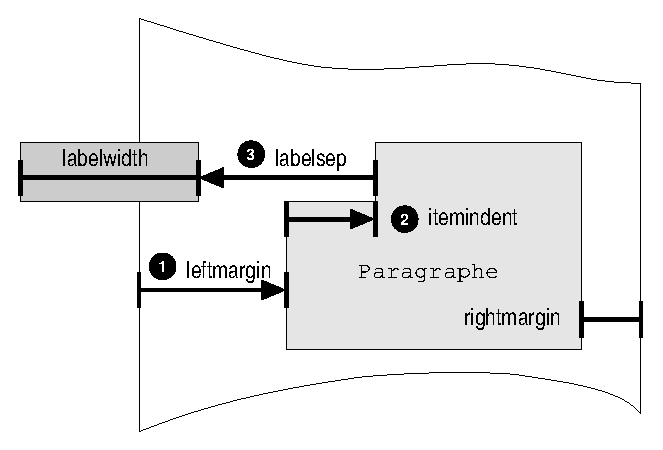
\includegraphics[width=0.4\linewidth]{img/liste-1}}
        \hspace{2cm}
        \subfloat[宽度大于\dm{\backslash labelwidth}]{%
          \label{fig:9.1b}
          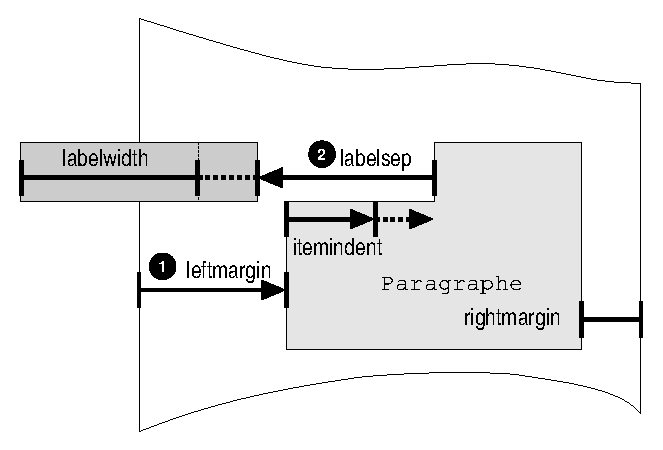
\includegraphics[width=0.4\linewidth]{img/liste-2}}
      \caption{列表入口的放置}
      \label{fig:9.1}
    \end{center}
\end{figure}

\subsection{纵向调整}

同样,我们也可以调整环境\dm{list}中的纵向空白,尤其是借助以下参数可以定义构成列表入口的段落间的距离,也可以定义我们想在列表前后插入的空白。

\begin{itemize}
  \item \verb|\itemsep|:列表各入口间的距离。
  \item \verb|\parsep|:列表入口内部的段落间距。
  \item \verb|\topsep|:所创建的环境前后插入的空白。如果新环境创建了新段落,距离还会再加上\verb|\partopsep|。
\end{itemize}

\subsection{默认值}

环境\dm{list}的所有参数都带有默认值。在鄙人的系统中用于在水平调整的长度默认值如下:

\begin{center}
  \begin{tabular}{|l|c|}
    \hline
    尺寸 & 默认值\\
    \hline
    \verb+\itemindent+    &0pt\\
    \verb+\listparindent+ &0pt\\
    \verb+\rightmargin+   &0pt\\
    \verb+\leftmargin+    &25pt\\
    \verb+\labelwidth+    &20pt\\
    \verb+\labelsep+      &5pt\\
    \hline
  \end{tabular}
\end{center}

用于纵向调整的长度的默认值如下:

\begin{center}
  \begin{tabular}{|l|c|}
    \hline
    尺寸 & 默认值\\
    \hline 
    \verb+\itemsep+       &4.0pt plus 2.0pt minus 1.0pt\\
    \verb+\parsep+        &4.0pt plus 2.0pt minus 1.0pt\\
    \verb+\topsep+        &8.0pt plus 2.0pt minus 4.0pt\\
    \verb+\partopsep+     &2.0pt plus 1.0pt minus 1.0pt\\
    \hline
  \end{tabular}
\end{center}

指令\verb|\makelabel|定义为:

\begin{dmd}
\verb+\hfil #1+
\end{dmd}

因此,在宽度为\verb|\labelwidth|的字盒中,项目标签的内容会被推向右侧。这样一来,如果我们使用以下方式定义一个简单列表:

\begin{dmd}
\begin{verbatim}
\newenvironment{listebasique}
{\begin{list}{}{}}
{\end{list}}
\end{verbatim}
\end{dmd}

那么对于带有项目标签的列表,可以这样使用它:

\newenvironment{listebasique}
{\begin{list}{}{}}
{\end{list}}

\begin{codelist}[9.16]{
    前文前文前文前文前文前文前文前文前文前文前文
    前文前文
    \begin{listebasique}
        \item[X]  o o o o o o o o o o o o o o
            o o o o o o o o o o o o o o o o o
          
            u u u u u u u u u u u u u u u u u
        \item[一个东西] v v v v v v v v v v v
    \end{listebasique}
    后文后文后文后文后文后文后文后文后文后文后文
    后文后文后文
}\begin{verbatim}
前文前文前文前文前文前文前文前文前文前文前文
前文前文
\begin{listebasique}
    \item[X]  o o o o o o o o o o o o o o
        o o o o o o o o o o o o o o o o o
      
        u u u u u u u u u u u u u u u u u
    \item[一个东西] v v v v v v v v v v v
\end{listebasique}
后文后文后文后文后文后文后文后文后文后文后文
后文后文后文
\end{verbatim}
\end{codelist}

对于没有列表标签的情况,则可以这样使用:

\begin{codelist}[9.17]{
    前文前文前文前文前文前文前文前文前文前文前文
    前文前文
    \begin{listebasique}
        \item[] e e e e e e e e e e e e e e e e
            e e e e e e e e e e e e e e e e e e
    \end{listebasique}
    后文后文后文后文后文后文后文后文后文后文后文
    后文后文后文
}\begin{verbatim}
前文前文前文前文前文前文前文前文前文前文前文
前文前文
\begin{listebasique}
    \item[] e e e e e e e e e e e e e e e e
        e e e e e e e e e e e e e e e e e e
\end{listebasique}
后文后文后文后文后文后文后文后文后文后文后文
后文后文后文
\end{verbatim}
\end{codelist}

\subsection{示例}

B.2节中,描述\LaTeX 辅助文件的列表是使用如下代码生成的:

\newenvironment{ficaux}{% 
\begin{list}{}{%
    % largeur de la boîte englobant le label :
          \setlength{\labelwidth}{1cm}
    % espace entre paragraphe et l ’ étiquette :
          \setlength{\labelsep}{8pt}
    % marge de gauche :
    \setlength{\leftmargin}{\labelwidth+\labelsep} \renewcommand{\makelabel}[1]{% production de l’étiquette : 
    \framebox[\labelwidth]{\texttt{##1}}}}}{\end{list}}

\begin{codelist}[9.18]{
    \begin{ficaux}
        \item[tex] \LaTeX{} 源文件,吧啦
        吧啦吧啦……
        \item[aux] 辅助文件……
        \item[log] 跟踪……
        \item[dvi] \emph{独立于设备}的文
        件……
    \end{ficaux}
}\begin{verbatim}
\begin{ficaux}
    \item[tex] \LaTeX{} 源文件,吧啦
    吧啦吧啦……
    \item[aux] 辅助文件……
    \item[log] 跟踪……
    \item[dvi] \emph{独立于设备}的文
    件……
\end{ficaux}
\end{verbatim}
\end{codelist}

环境\dm{ficaux}按如下方式定义:

\begin{dmd}
\begin{verbatim}
\newenvironment{ficaux}{% 
    \begin{list}{}{%
        % 包含整个标签的字盒宽度:
        \setlength{\labelwidth}{1cm}
        % 段落和项目标签的间距:
        \setlength{\labelsep}{8pt}
        % 左边距:
        \setlength{\leftmargin}{\labelwidth+\labelsep} 
        \renewcommand{\makelabel}[1]{% 生成项目标签:
            \framebox[\labelwidth]{\texttt{##1}}}}}{\end{list}}
\end{verbatim}
\end{dmd}

在这个例子中,以下关系使得列表入口的位置按图\ref{fig:9.2a}所示的方式确定:

\begin{dmd}
\verb|\leftmargin=\labelwidth+\labelsep|
\end{dmd}

%TODO 与附录统一

\begin{figure}[ht]
    \begin{center}
        \leavevmode \subfloat[\dm{ficaux}列表]{%
          \label{fig:9.2a}
          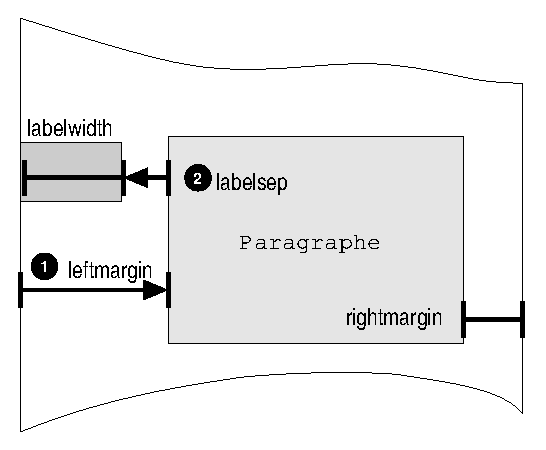
\includegraphics[width=0.4\linewidth]{img/liste-ficaux}}
        \hspace{2cm}
        \subfloat[\dm{question}列表]{%
          \label{fig:9.2b}
          \includegraphics[width=0.4\linewidth]{img/liste-question.eps}}
      \caption{示例列表的项目标签位置}
      \label{fig:9.2}
    \end{center}
\end{figure}

再看一个例子:创建一个带编号的列表环境,为实验课或课堂测验生成试卷题目……

\newcounter{cptquestion}

\newcommand{\etiquettequestion}[1]{% 
\makebox[\labelwidth]{%
     \Pisymbol{pzd}{47}$_\thecptquestion$}}

\newenvironment{question}{\begin{list}{}{%
    \usecounter{cptquestion}% 
    \setlength{\labelwidth}{2em}% 
    \setlength{\labelsep}{1em} 
    \setlength{\itemindent}{15pt}% 
    \setlength{\leftmargin}{.8cm} 
    \setlength{\rightmargin}{10pt} 
    \renewcommand{\makelabel}[1]{%
        \etiquettequestion{##1}}}}
{\end{list}}

\begin{codelist}[9.19]{
    \begin{question}
        \item o o o o o o o o o o o o o o o o
            o o o o o o o o o o o o o o o o o
        \item o o o o o o o o o o o o o o o o
            o o o o o o o o o o o o o o o o o
            o o o o o o o o o o o o o o o o o
        \item o o o o o o o o o o o o o o o o
            o o o o o o o o o o o o o o o o o
    \end{question}
}\begin{verbatim}
\begin{question}
    \item o o o o o o o o o o o o o o o o
        o o o o o o o o o o o o o o o o o
    \item o o o o o o o o o o o o o o o o
        o o o o o o o o o o o o o o o o o
        o o o o o o o o o o o o o o o o o
    \item o o o o o o o o o o o o o o o o
        o o o o o o o o o o o o o o o o o
\end{question}
\end{verbatim}
\end{codelist}

该环境可以由以下代码生成:

\begin{dmd}
\begin{verbatim}
    \newenvironment{question}{\begin{list}{}{% 
        \usecounter{cptquestion}% 
        \setlength{\labelwidth}{2em}% 
        \setlength{\labelsep}{1em} 
        \setlength{\itemindent}{15pt}% 
        \setlength{\leftmargin}{.8cm} 
        \setlength{\rightmargin}{10pt} 
        \renewcommand{\makelabel}[1]{%
            \etiquettequestion{##1}}}}
   {\end{list}}
\end{verbatim}
\end{dmd}

对应的位置确定过程如图\ref{fig:9.2b}所示。注意到,在列表的定义中,指令\verb|\usecounter|用来创建编号,并且指明了会用到的计数器。因此,需要声明所涉及的计数器:

\begin{dmd}
\verb+\newcounter{cptquestion}+
\end{dmd}

接下来,每个列表入口由题号和一个“美观”的铅笔图标构成,可以借助以下指令来达到我们的目的:

\begin{dmd}
\begin{verbatim}
\newcommand{\etiquettequestion}[1]{% 
    \makebox[\labelwidth]{%
        \Pisymbol{pzd}{47}$_\thecptquestion$}}
\end{verbatim}
\end{dmd}

最后,以下指令重定义了指令\verb|\makelabel|:

\begin{dmd}
\verb|\renewcommand{\makelabel}[1]{\etiquettequestion{##1}}}}|
\end{dmd}

这样的重定义使其调用我们“美观”的铅笔图标。指令\verb|\etiquettequestion|的第一个也是唯一一个参数由表达式\verb+##1+传入。实际上,在定义环境\dm{question}的语境中,\verb|#1|就成为了该语境的第一个参数。

本书附录B中可以找到包的列表。生成这个列表的代码如下:

\begin{dmd}
\begin{verbatim}
\newenvironment{packages}{\begin{list}{}{%
    \setlength{\labelwidth}{2.5cm}%
    \setlength{\itemindent}{0pt}% 
    \setlength{\leftmargin}{\labelwidth+\labelsep}% 
    \renewcommand{\makelabel}[1]{%
        $\blacktriangle$ \ltxpack{##1} \hfil:}}}
    {\end{list}}
\end{verbatim}
\end{dmd}

\newenvironment{packages}{\begin{list}{}{%
    \setlength{\labelwidth}{2.5cm}%
    \setlength{\itemindent}{0pt}% 
    \setlength{\leftmargin}{\labelwidth+\labelsep}% 
    \renewcommand{\makelabel}[1]{%
        % $\blacktriangle$ \textsf{##1} \hfil:}}}
        \textsf{##1} \hfil:}}}
    {\end{list}}
%FIXME ▲不显示

其中,指令\verb|\ltxpack|的定义见11.1.2小节。为了给你提供更多信息,该环境的效果如下:

\begin{codelist}[9.20]{
    \begin{packages}
        \item[▴\ 某东西] 该包可以用于在文档中插入
        某东西,而不需要这个玩意和那个物件……
    \end{packages}
}\begin{verbatim}
\begin{packages}
    \item[某东西] 该包可以用于在文档中插入
    某东西,而不需要这个玩意和那个物件……
\end{packages}
\end{verbatim}
\end{codelist}

\subsection{略微变形的示例}

我们接下来围绕本书术语词典的组成方法来讨论细节。这个例子中的列表风格展示在接下来说明两个思路的列表中:

\newcommand{\boiteentreeglossaire}[1]{% 
\parbox[b]{\labelwidth}{%
\setlength{\fboxsep}{3pt}% 
\setlength{\fboxrule}{.4pt}% 
\shadowbox{\sffamily#1}\\\hfill\mbox{}}}

\newenvironment{glossaire}{\begin{list}{}{%
     \setlength{\labelwidth}{.5\textwidth}% 
     \setlength{\labelsep}{-.8\labelwidth}% 
     \setlength{\itemindent}{\parindent}% 
     \setlength{\leftmargin}{25pt}% 
     \setlength{\rightmargin}{0pt}%
     \setlength{\itemsep}{.8\baselineskip}% 
     \renewcommand{\makelabel}[1]{%
       \boiteentreeglossaire{##1}}}}
{\end{list}}

\begin{glossaire}
    \item[思路1] 长度\verb|\labelsep|可以是负值,这样可以使列表入口和段落重合,如图\ref{fig:9.3a}所示。
    \item[思路2] 我们可以创建一个段落字盒,用于创建项目标签。这样创建的字盒可以由两行文字构成,上面的一行是构成项目标签文本的文字,下面的一行置空并与段落重合,如图\ref{fig:9.3b}所示。
\end{glossaire}

\begin{figure}[ht]
    \begin{center}
        \leavevmode \subfloat[\dm{\backslash labelsep}使用负值]{%
          \label{fig:9.3a}
          \includegraphics[width=0.4\linewidth]{img/liste-glo-1}}
        \hspace{2cm}
        \subfloat[创建段落字盒使项目标签和段落重叠]{%
          \label{fig:9.3b}
          \includegraphics[width=0.4\linewidth]{img/liste-glo-2}}
      \caption{列表“术语字典”中项目标签的位置确定}
      \label{fig:9.3}
    \end{center}
\end{figure}

本书使用的生成如上形式的列表和其中项目标签的代码如下:

\begin{dmd}
\begin{verbatim}
\newenvironment{glossaire}{\begin{list}{}{%
    \setlength{\labelwidth}{.5\textwidth}% 
    \setlength{\labelsep}{-.8\labelwidth}% 
    \setlength{\itemindent}{\parindent}% 
    \setlength{\leftmargin}{25pt}% 
    \setlength{\rightmargin}{0pt}%
    \setlength{\itemsep}{.8\baselineskip}% 
    \renewcommand{\makelabel}[1]{%
        \boiteentreeglossaire{##1}}}}
{\end{list}}
\end{verbatim}
\end{dmd}

\verb|\itemsep|的值\verb|.8\baselineskip|针对每个列表入口插入了空白,可以项目标签“透透气”。
\chapter{装饰}

\begin{quote}
    我说,我要上这棕树,抓住枝子。愿你的两乳好像葡萄累累下垂,你鼻子的气味香如苹果。你的口如上好的酒,女子说,为我的良人下咽舒畅,流入睡觉人的嘴中。

    \hfill《圣经·雅歌》7:10
\end{quote}

那本章的主要思路是介绍,介绍那些为生成文档中个别部分而被个性化修改的\LaTeX 的标准工具,间或可以从中看到些用于“调香”的宏。这些个性化设置可以应用于各个层级:使用包的选项,如设置页眉;偶尔涉足宏定义,如设置章节的展现风格;更深入地处理宏,如处理内容的表格。本章的一部分聚焦于我们可以从包\textsf{fancyvrb}中调用的工具。作为本章的末尾,我们会去抨击一下法文的引号。

\section{索引的外观} % 这节翻译得是什么破玩意

为了修改索引的外观,需要明白,当我们大手一挥噼里啪啦地写下如下指令的时候,我们实际上就生成了一个文件\codereplace{文档}\dm{.ind}:

\dmh{makeindex }\codereplace{文档}

该文件包含了类似下面列出的内容:

\begin{dmd}
\verb|\begin{theindex}| \quad$\leftarrow$\textsf{文前部分}\\
~\\
\verb|\item Cosmic debris, 12,34|\\
~\\
\verb|\indexspace| \quad$\leftarrow$\textsf{分组间的空间}\\
~\\
\verb|\item Debra kadabra, 23| \quad$\leftarrow$\textsf{入口,分割符,页码}\\
~\\
\verb|\end{theindex}| \quad$\leftarrow$\textsf{文后部分}
\end{dmd}

实际上,该代码会从带有预定义值且可被修改的一般性实体中生成。为了证明这个观点,只需要知道,程序\textsf{makeindex}可以生成一个包含\LaTeX 代码外内容的\dm{.ind}文件。为了理解一般性实体的职责,可以用如下方式描述\textsf{makeindex}的工作。

\begin{enumerate}
    \item 根据实体\dm{preamble}的值来写入文前部分。
    \item 对于每个\dm{.idm}文件:
    \begin{enumerate}
        \item 写入实体\dm{item\_0}的内容;
        \item 写入入口(本例中为“Cosmic debris”);
        \item 写入分割符(实体\dm{delin\_0}的值);
        \item 写入页码。
    \end{enumerate}
    \item 在每个分组的结尾(即首字母切换时),写入实体\dm{group\_skip}的内容;
    \item 根据\dm{postamble}的值写入文后部分。
\end{enumerate}

上述实体的默认值如下:

\begin{center}
    \begin{dmd}
        \begin{tabular}{|l|l|}
            \hline
            preamble & \verb+"\\begin{theindex}\n"+\\
            item\_0 &\verb+"\n \\item"+\\
            delim\_0 & ", "\\
            group\_skip & \verb+"\n\n \\indexspace\n"+\\
            postamble & \verb+"\n\n\\end{theindex}\n"+\\
            \hline
        \end{tabular}
    \end{dmd}
\end{center}

这些值可以使用通常带有后缀名\dm{.ist}的风格文件作为媒介来修改。可以通过以下方式在调用\textsf{makeindex}时使用:

\dmh{makeindex -s \codereplace{风格}.ist \codereplace{文件}}

如此一来,为了生成文档的标题,我们可以一开始就重新定义一二级间的分隔符:

\begin{dmd}
\begin{verbatim}
delim_0 " \\dotfill \ "
delim_1 " \\dotfill \ "
\end{verbatim}
\end{dmd}

我们将默认用于分隔索引入口和页码的逗号替换成了省略号。接下来,通过严谨地阅读\textsf{makeindex}的文档\jz{
    可参见参考文献的实用引用后的提醒。
},可以注意到要求\textsf{makeindex}为入口组和代表分组的字母间生成空间的礼貌方式如下:

\begin{dmd}
headings\_flag 1
\end{dmd}

这里,代表分组的字母会表示为大写,并且借助实体\dm{heading\_prefix}和\dm{heading\_suffix}的内容框起。无所谓——为了生成我们美丽的带阴影的字盒,我们可以在风格文件中这样写:

\begin{dmd}
\begin{verbatim}
heading_prefix "{\\large\\sffamily\\bfseries\\shadowbox{"
heading_suffix "}\\hfill}\\nopagebreak\n"
\end{verbatim}
\end{dmd}

这段你已经可以看懂的示例内容,就会生成我们需要的字盒。例如对于字母C:

\begin{codelist}[10.1]{
    {\large\sffamily\bfseries%
    \shadowbox{C}\hfil}\nopagebreak
}\begin{verbatim}
{\large\sffamily\bfseries%
    \shadowbox{C}\hfil}\nopagebreak
\end{verbatim}
\end{codelist}

这段指令会被\dm{group\_skip}的内容覆盖掉。而我们稍早前说过,\dm{group\_skip}的默认值是\verb|\indexspace|。在研究了几个月之后\jz{
    开玩笑的。我是想说,只花了几秒……好吧,几分钟。
},我们成功地在\dm{book.cls}中发现了该指令的定义,并且将分组间空间略微扩大了些:

\begin{dmd}
\renewcommand\indexspace{%
    \par \vskip 20pt plus5pt minus3pt\relax}
\end{dmd}

\begin{ii}
本小节中,我们只是非常简单地看了看makeindex提供的功能。除了在《\LaTeX 伴侣》中能找到的信息,Debian环境下关于此工具的说明书中提供了我们可以定义的一半入口的详尽列表。由P.陈(P. Chen;音译)和M.A.哈林森(M. A. Harrinson)编写的文件\dm{ind.dvi}同样是初学索引自定义的良好开端。
\end{ii}

\section{标题的外观}

在本节,我们会介绍我们修改\LaTeX 标准(篇、章、节等)标题外观的方式。

\subsection{目录中的编号}

作为开始操作目录的前提条件,需要掌握两个计数器:

\begin{enumerate}
    \item \dm{secnumdepth}(英:\emph{section numbering depth}),可以明确文档中标题编号的层级;
    \item \dm{tocdepth}(英:\emph{table of contents depth}),可以定义目录标题的最大层级(或称最大深度)。
\end{enumerate}

为了使用这两个计数器,还需要了解\LaTeX 为各标题连接层级的方法。以下是各标题的层级:

\begin{center}
    \begin{tabular}{|c|r||c|r|}
        \hline
        标题 & 层级 & 标题 & 层级\\
        \hline
        \dm{part} & -1 & & \\
        \dm{chapter}    & 0 & \dm{subsubsection} & 3\\
        \dm{section}    & 1 & \dm{paragraph}     & 4\\
        \dm{subsection} & 2 & \dm{subparagraph}  & 5\\
        \hline
    \end{tabular}
\end{center}

如此一来,将\verb|secnumdepth|赋值为1、将\verb|tocdepth|赋值为2,则可以让标题编号至各\verb|\section|,同时将层级少于\verb|\subsection|的标题插入目录。

\subsection{节和更少的层级}

在\TeX 系统的文件\dm{book.cls}中,我们可以找到如下代码\jz{
    稍微简化了一些……
}:

\begin{dmd}
\begin{verbatim}
\newcommand{\section}{%
    \@startsection%
    {section} % 标题名称
    {1} % 标题层级
    {0pt} % 缩进
    {-3.5ex plus -1ex minus -.2ex}% 段前纵向空间
    {2.3ex plus.2ex}% 段后纵向空间{\normalfont\Large\bfseries}} % 标题外观
\end{verbatim}
\end{dmd}

该段代码定义了节标题的生成方式。可以观察到,指令\verb|\section|调用了指令\verb|\@startsection|,而后者需要6各参数:

\begin{itemize}
    \item 标题名称,如\dm{section}、\dm{subsection}等;
    \item 标题层级,1对应\dm{section},2对应\dm{subsection},3对应\dm{subsubsection},等等;
    \item 缩进;
    \item 标题前的纵向空白;
    \item 标题后的纵向空白;
    \item 用于确定标题本身格式的一系列\emph{声明}。
\end{itemize}

因此,我们可以注意到\LaTeX 默认为类型\dm{book}设定的版式如下。

\begin{itemize}
    \item 无缩进(\dm{0pt})。
    \item 标题前的纵向空间为\dm{3.5ex},带有正向\dm{-1ex}和负向\dm{-.2ex}的允差。
    \item 标题后的纵向空间为\dm{2.3ex},带有正向\dm{.2ex}的允差。可以注意到,如果空间为负,则段落开头会紧接标题,而不会重起一段。
    \item 标题加粗加大,使用“常规”(normal)字体。
\end{itemize}

为了定义本文档使用的标题样式,我们引入三个长度,分别用于\dm{section}、\dm{subsection}、\dm{subsubsection}的缩进:

\begin{dmd}
\begin{verbatim}
\newlength{\sectiontitleindent}
\newlength{\subsectiontitleindent}
\newlength{\subsubsectiontitleindent}
\end{verbatim}
\end{dmd}

长度值如下:

\begin{dmd}
\begin{verbatim}
\setlength{\sectiontitleindent}{-1cm}
\setlength{\subsectiontitleindent}{-.5cm}
\setlength{\subsubsectiontitleindent}{-.25cm}
\end{verbatim}
\end{dmd}

此外,我们为标题还定义了特殊的字体,具体如下:

\begin{dmd}
\begin{verbatim}
\newcommand{\sectionfont}{% 
    \fontencoding{\encodingdefault}% 
    \fontfamily{pag}% \fontseries{bc}%
    \fontshape{n}% \selectfont}
\end{verbatim}
\end{dmd}

该指令可以选用PostScript字体AvantGarde的加粗紧缩版本(参阅9.4节)%TODO 解释中文的使用
。最终,我们使用了以下指令来定义节标题外观:

\begin{dmd}
\begin{verbatim}
\renewcommand{\section}{% 
    \@startsection%
    {section}%
    {1}%
    {\sectiontitleindent}%
    {-3.5ex plus -1ex minus -.2ex}% 
    {2.3ex plus.2ex}% {\sectionfont\Large}}
\end{verbatim}
\end{dmd}

对于更少层级的标题,我们也编写了等价的指令。

\subsection{章}

通过深入研究文件\dm{book.cls},我们可以找到有关\LaTeX 生成章首内容的信息。

\subsubsection{原则}

在文件\dm{book.cls}中,我们可以找到以下指令:

\begin{dmd}
\begin{verbatim}
\newcommand{\chapter}{% 
    ...
    \thispagestyle{plain}%
    ...
    \secdef\@chapter\@schapter} % 我们感兴趣的行
\end{verbatim}
\end{dmd}

指令\verb|\chapter|本身会调用两个不同的指令:

\begin{enumerate}
    \item \verb|\@chapter|,用于被编号的章标题;
    \item \verb|\@schapter|,用于不被编号的章标题(\dmh{s}代表\emph{star},即“星号”,对应指令\verb|\chapter*|)。
\end{enumerate}

在英勇地(同样在文件\dm{book.cls}中)查找这两条指令的定义之后,我们找到了下面这类东西:

\begin{dmd}
\begin{verbatim}
\def\@chapter[#1]#2{% ...
    \refstepcounter{chapter}%
    % 终端上的消息:
    \typeout{\@chapapp\space\thechapter.} 
    \addcontentsline{toc}{chapter}% 在目录中添加标题
    ...
    \if@twocolumn
    ...
    \else% 针对不分栏的文档
    \@makechapterhead{#2}% 我们感兴趣的代码行
    \fi}
\end{verbatim}
\end{dmd}

这段代码把我们领上道了……实际上,\verb+\@makechapterhead+(可以按字面翻译为“制作章首装饰”)正是我们更改图案所需要重定义的指令。经过进一步的搜索,我们可以发现指令\verb|\@makeschapterhead|能够生成未编号的章首装饰。这两条指令接受章名作为其参数。

\subsubsection{必要的小工具}

我们定义了环境\dm{cadrechap},用于简单地讲右边距加宽2厘米:

\begin{dmd}
\begin{verbatim}
\newenvironment{cadrechap}% 
    {\begin{list}{}{%
        \setlength{\leftmargin}{0pt}% 
        \setlength{\rightmargin}{-2cm}% 宽敞些
        \setlength{\itemindent}{0pt}% 
        \setlength{\labelsep}{0pt}%
    }\item}% 
{\end{list}}
\end{verbatim}
\end{dmd}

同时,可以使用布尔值\dm{@mainmatter}来获取我们目前是否处于文档的“中心”——这是针对指令\verb|\mainmatter|被调用的情况。

\subsubsection{严格的章首装饰}

本文档中,生成章首装饰的指令可以看作两个微型页面的组合。%TODO minipage

\begin{enumerate}
    \item 在左侧的是微型页面字盒。我们指定了它的高度,以便放置微型摘要(参见\S 10.7)。
    \item 在右侧的是包含“章”一词和章号的字盒。
\end{enumerate}

\newcommand{\boite}[1]{%
  {\setlength{\fboxrule}{.2pt}%
    \setlength{\fboxsep}{-\fboxrule}%
    \fbox{#1}}}
\DeclareFixedFont{\fnumfont}{T1}{phv}{b}{n}{32pt}
\DeclareFixedFont{\fnomfont}{T1}{phv}{b}{n}{12pt}
\DeclareFixedFont{\ftitrefont}{T1}{phv}{b}{n}{16pt}

\newcommand{\fairechapitre}[1]{%
  \noindent\begin{minipage}{\linewidth}%
      \boite{\begin{minipage}[t][3cm][c]{.75\textwidth}%
          \centering%
          为\\微型摘要\\准备的\\微型页面
        \end{minipage}}%
      \boite{\begin{minipage}[t]{.25\textwidth}
          \begin{flushright}
            {\fnomfont\chaptername}\\[.5cm]
            {\fnumfont\thechapter}
          \end{flushright}
        \end{minipage}}
    \end{minipage}\par
  \begin{flushright}\ftitrefont#1\end{flushright}}

\fairechapitre{Zhang biaoti}%TODO  font

实现此类字盒组合的框架如下:

\begin{dmd}
\begin{verbatim}
\begin{cadrechap}
    \begin{minipage}[t][6cm][t]{0.75\linewidth}
        % 这里插入微型摘要 
    \end{minipage} 
    \begin{minipage}[t]{0.25\linewidth}
        % 这里插入章号
    \end{minipage}
    \begin{flushright}
        % 这里插入章标题
    \end{flushright}
\end{cadrechap}
\end{verbatim}
\end{dmd}

此处无疑需要注意到,左侧的字盒(即接收微型目录的字盒)带有可指定的高度,用于以一致的方法来生成章首装饰而无须关注章中的节数(即无须关注微型目录的高度)。接下来,为不同元素定义不同的字体,就可以完成章首装饰的定义。在本文档中,我们的定义如下:

\begin{dmd}
\begin{verbatim}
% 章号
\DeclareFixedFont{\chapnumfont}{T1}{phv}{b}{n}{80pt}
% “章”一词
\DeclareFixedFont{\chapchapfont}{T1}{phv}{b}{n}{16pt}
% 章标题
\DeclareFixedFont{\chaptitfont}{T1}{phv}{b}{n}{24.88pt}
\end{verbatim}
\end{dmd}

\DeclareFixedFont{\chapnumfont}{T1}{phv}{b}{n}{80pt}
\DeclareFixedFont{\chaptitfont}{T1}{phv}{b}{n}{24.88pt}

因此,有如下指令:

\begin{codelist}[10.2]{
    {\chapnumfont 8}
    {\chaptitfont Oula !}
}\begin{verbatim}
{\chapnumfont 8}
{\chaptitfont Oula !}
\end{verbatim}
\end{codelist}

\subsection{部分}

在文件\dm{book.cls}中,我们可以找到指令\verb|\part|的定义:

\begin{dmd}
\begin{verbatim}
\newcommand\part{% 
    \cleardoublepage
    \thispagestyle{plain}
    [...]
    \null\vfil
    \secdef\@part\@spart}
\end{verbatim}
\end{dmd}

该定义告诉我们,正如各章一样,指令\verb|\part|会调用两条独立的指令,用于生成编号和不编号的部分(分别借助指令\verb|\@part|和\verb|\@spart|)。在之前的实践中,我们指定了页面的风格,使得各部分的开头为空(即没有页码和部分开头的装饰等),指令如下:

\begin{dmd}
\begin{verbatim}
\newcommand\part{%
    \cleardoublepage
    \thispagestyle{empty}% 代替默认的plain
    [...]
    \null\vfil% 空字盒和竖直方向的弹性空间
    \secdef\@part\@spart}
\end{verbatim}
\end{dmd}

接下来,我们可以查看指令\verb|\@part|的定义。该指令用于生成展示文档部分的页:

\begin{dmd}
\begin{verbatim}
\def\@part[#1]#2{%
    [...]
    {\centering % 居中
     [...]
     \huge\bfseries \partname\nobreakspace\thepart
        \par
        \vskip 20\pt
     [...]
     \Huge \bfseries #2\par}% 
\@endpart}
\end{verbatim}
\end{dmd}

通过查看这段代码,我们了解到,展现部分的页面由一行加粗加大的“部分”字样和部分的序号构成\jz{
    实际上,在联动了包\textsf{babel}和选项\dm{french}后,这两个指令会被重定义,以生成形如“Première partie”(第一部分)的内容。
}:

\begin{dmd}
\verb|\huge\bfseries \partname\nobreakspace\thepart|
\end{dmd}

在距离20点的下方,是部分的标题(存储在参数\verb|#2|中)。对于此文档,我们以如下方式重定义了指令\verb|\@part|:

\begin{dmd}
\begin{verbatim}
\def\@part[#1]#2{% 
    [...]
    {\centering
     \interlinepenalty \@M
     \normalfont
     [...]
     \partnumfont \thepart % 只显示部分的序号
     \par
     \vskip 50\p@% 将20点改为50点
     \partfont #2\par}% 使用自定义字体的标题
    \@endpart}
\end{verbatim}
\end{dmd}

为了与章首装饰保持一致,我们定义指定字体的指令如下:

\begin{dmd}
\begin{verbatim}
\newcommand{\partfont}{% 
    \fontencoding{\encodingdefault}\fontfamily{phv}% 
    \fontseries{bc}\fontshape{n}% \fontsize{32}{34}%
    \selectfont}
\DeclareFixedFont{\partnumfont}{T1}{phv}{bc}{n}{80}%
\end{verbatim}
\end{dmd}

\begin{exclamation}
我们也应注意到,指令\verb+\@part+依靠调用另一条指令作为结尾:\verb|\@endpart|。通过查看文件\dm{book.cls}可以看到,这样的结尾可以阻止来自指令\verb|\part|的纵向弹性空间,并跳过一个空白页……
\end{exclamation}

\section{几何}

本文档中,各页面中的不同尺寸借助包\textsf{geometry}使用如下指令定义:

\begin{dmd}
\begin{verbatim}
\geometry{%
    a4paper, 
    body={150mm,250mm}, 
    left=25mm,top=25mm, 
    headheight=7mm,headsep=4mm, marginparsep=4mm, 
    marginparwidth=27mm}
\end{verbatim}
\end{dmd}

这会分别定义如下元素(如图\ref{fig:10.1}所示):

\begin{itemize}
    \item 版心宽150 mm,高250 mm;
    \item 版心在页面上的位置为左边距25 mm、上边距25 mm;
    \item 页眉高7 mm,页眉与正文的间距为4 mm;
    \item 页面尺寸为标准A4;
    \item 用于页边注释的页边距为2.7 cm。
\end{itemize}

\begin{figure}[ht]
    \centering
    \includegraphics{img/geometry}
    \caption{定义文档几何样式的部分尺寸}
    \label{fig:10.1}
\end{figure}

以通常的方式来讲,正如图\ref{fig:10.1}展现的,包\textsf{geometry}可以定义一定数量的尺寸。我们可以以选项的方式将这些尺寸传递给\verb|\usepackage|,也可以借助指令\verb|\geometry|。

\begin{description}
    \item[页面尺寸]%TODO 此处如何换行,下同
    
\begin{itemize}
    \item 若使用预定义中的格式,可以使用\dm{a4paper}、\dm{a5paper}等。
    \item 若要自由地指定纸张尺寸,例如针对会使用碎纸机销毁的文档的尺寸,可以使用\dm{paperwidth=}\codereplace{尺寸}和\dm{paperheight=}\codereplace{尺寸}。
\end{itemize}

\item[文本]

\begin{itemize}
    \item 可以使用\dm{body=\{\codereplace{宽度},\codereplace{高度}\}};
    \item 也可以使用\dm{width=}\codereplace{宽度}和\dm{height=}\codereplace{高度};
    \item 文本在页面内的位置由参考点确定,可以使用\dm{top=}\codereplace{纵向位置}和\dm{left=}\codereplace{水平位置}确定参考点位置。
\end{itemize}

\item[页面顶端和底部]

\begin{itemize}
    \item 页面中为页面预留的高度可以借助神奇的表达式\dm{headheight=}\codereplace{高度}定义,页眉相对于版心的位置可以借助指令\dm{headsep=}\codereplace{空间}指定;
    \item 页脚的位置可以通过长度\dm{footskipp=}\codereplace{空间}指定,该长度可以定义版心底部和页脚第一行间的空间。
\end{itemize}

\item[页边注释] 秉承着同样的精神,页面中为边注预留的空间的宽度和位置可以借助两个长度定义:\dm{marginparwidth=}\codereplace{宽度}和\dm{marginparsep=}\codereplace{空间}
\end{description}

\begin{exclamation}
包geometry中,涉及页眉、页脚、边注的尺寸默认算作版心\emph{外}的部分。有一些指令可以将这些尺寸中的一个或多个包含到版心内部来完成计算。例如,我们可以说“我希望版心宽度为10厘米,包含边注”。关于更多相关细节,请参阅包文档。
\end{exclamation}

\section{页眉和页脚}

版心上下的空间分别成为页眉和页脚,可以借助包\textsf{fancyhdr}来定制。定制的基本原则很简单\jz{
    在读完接下来的内容后,你无疑会开始质疑这里说的“简单”一词……
},只需要使用以下指令来指明我们想要使用借助包\textsf{fancyhdr}定义的页眉和页脚。该包默认会在页面下方和页脚上方生成一条水平线段,线段粗细分别由\verb|\footrulewidth|和\verb|\headrulewidth|定义。接下来,我们使用以下指令:

\begin{itemize}
    \item \verb|\fancyhead|,来定义页眉;
    \item \verb|\fancyfoot|,来定义页脚。
\end{itemize}

这两条指令都可以接收由一个或两个以下字符组成的序列构成的参数:

\begin{itemize}
    \item \dm{E}或\dm{O},用于指明页码的奇偶性(偶数即\emph{even},奇数即\emph{odd});
    \item \dm{R}、\dm{L}或\dm{C},用于指明我们想在哪个位置生成信息,分别指代右侧、左侧或居中。
\end{itemize}

示例如下:

\begin{dmd}
\begin{verbatim}
\fancyhf{} % 清除页面并开始
% 【页眉】
% 作者姓名首字母偶数页靠右,奇数页靠左:
\fancyhead[RE,LO]{VL}
% 页码居中:
\fancyhead[C]{\thepage}
% 节号奇数页靠右,
% 偶数页靠左:
\fancyhead[LE,RO]{\thesection}
% 【页脚】
% 图片奇数页靠右,偶数页靠左:
\fancyfoot[RO,LE]{\includegraphics[height=4ex]{punch}}
% 标题奇数页靠右,偶数页靠左:
\fancyfoot[LO,RE]{%
    关于\LaTeX{}的那些你想知道的问题}
% 线条粗细
\renewcommand{\footrulewidth}{3pt}
\end{verbatim}
\end{dmd}

\fancyhf{} 
\fancyhead[RE,LO]{VL}
\fancyhead[C]{\thepage}
\fancyhead[LE,RO]{\thesection}
\fancyfoot[RO,LE]{\includegraphics[height=4ex]{punch}}
\fancyfoot[LO,RE]{关于\LaTeX{}的那些你想知道的问题}
\renewcommand{\footrulewidth}{3pt}

\subsection{章首页的情况}

在类型\dm{book}中,\LaTeX 会自动为每章的第一页调用风格\dm{plain}。为了使包\textsf{fancyhdr}为这些页面定义新风格,可以使用如下指令:

\begin{dmd}
\begin{verbatim}
% 章首页的情况 
\fancypagestyle{plain}{%
    \fancyhf{}% 全部清空 
    \fancyfoot[C]{\thepage}% 页面底部的页码
    % 清空所有线条
    \renewcommand{\headrulewidth}{0pt}% 
    \renewcommand{\footrulewidth}{0pt}}
\end{verbatim}
\end{dmd}

可以注意到,本书各章的章首正是采用了这种风格……

\subsection{章首前的空白页}

在类型\dm{book}的双面模式下(正是本文档对应的情况),\LaTeX 会默认在奇数页——这在排版术语中称作“单面”(belle page)——开始新的一章。为了实现这一点,\LaTeX 在不同的内部指令中调用了指令\verb+\cleardoublepage+。这样可以在必要时在章的首页前插入一个空白页。默认情况下,该空白页会带有目前使用的页眉和页脚。在本文档中,我们针对这些页面修改了文件\dm{latex.ltx}中的指令\verb|\cleardoublepage|,指定了一种“空白”的风格:%TODO 还没搞

\begin{dmd}
\begin{verbatim}
\renewcommand{\cleardoublepage}{% 重定义该指令
    \clearpage\ifodd\c@page\else
    \hbox{}
    \vspace*{\fill}
    \thispagestyle{empty}% 添加此行 
    \newpage
    \fi}
\end{verbatim}
\end{dmd}

你可以翻阅本书,看看章首前的页面是否是空白的……

\subsection{标记的机制}

你无疑已经注意到了,本书的页眉带有一些与文本相关的内容。实际上,针对偶数页(出现在左侧的页面),我们插入了章标题;针对奇数页(出现在右侧的页面),我们插入了该页出现的最后一节的节标题。\LaTeX 部署了一种\emph{标记}机制,使得我们可以实现这一点。这里将尝试解释这种机制。

\begin{exclamation}
这里不妨解释一下:\LaTeX 和\TeX 生成一个页面是,它们会根据从所涉页面收集来的信息来制备页眉和页脚。因此,生成页眉和页脚是编译页面的后置步骤。
\end{exclamation}

\subsubsection{指令\dm{\backslash markboth}和\dm{\backslash markright}}

设有以下指令:

\begin{dmd}
\backslash markboth\{\codereplace{文本$_{\mbox{左}}$}\}\{\codereplace{文本$_{\mbox{右}}$}\}
\end{dmd}

或:

\begin{dmd}
\backslash markright\{\codereplace{文本}\}
\end{dmd}

想象参数\codereplace{文本$_{x}$}存储在栈和队列中。根据这种想法,有:

\begin{itemize}
    \item \verb|\markboth|将\codereplace{文本$_{\mbox{左}}$}入栈,将\codereplace{文本$_{\mbox{右}}$}存入队列;
    \item \verb|\markright|将\codereplace{文本}存入队列。
\end{itemize}

在一个页面中,这两个“标记”指令可以调用多次,也可以一次都不调用。在\TeX 结束版心的排版,在生成页眉和页脚时,会探索栈和队列的参数。这借助了以下指令:

\begin{itemize}
    \item \verb|\leftmark|返回栈顶,即\emph{上一次调用}\verb|\markboth|时的\codereplace{文本$_{\mbox{左}}$};
    \item \verb|\rightmark|返回队列头,即\emph{第一次调用}\verb|\markboth|时的\codereplace{文本$_{\mbox{右}}$},或\emph{第一次调用}\verb|\markbot|时的\codereplace{文本}。
\end{itemize}

\begin{exclamation}
我们这里介绍的“队列”有一个小巧思:只要页面中没有“标记”指令添加数据,那么队列就会保持此前的页面中\emph{最后插入的信息}。指令\verb|\markboth|和\verb|\markright|一出现,“队列”就被清空。
\end{exclamation}

另一个理解这种标记机制的方法可以描述如下:

\begin{itemize}
    \item \verb|\leftmark|包含入栈的最后一条信息(借助\verb|\markboth|的第一个参数);
    \item 如果我们在页面上放置了一词\verb|\rightmark|,则它包含“队列”的第一条信息,否则它包含队列中的最后一条信息(借助\verb|\markboth|的第二个参数或\verb|\markright|的参数)。
\end{itemize}

\begin{ii}
    供你参考的是,作者使用了这些指令来生成了带有几十个名称和照片的相册。这里的思路是去探索通过页眉显示页面上第一个和最后一个名称的机制——这种页眉跟字典很像。为了实现这个目的,只需要为每个人(包含名称和照片)调用以下指令:
    
    \begin{dmd}
    \backslash markboth\{\codereplace{老铁的名称}\}\{\codereplace{老铁的名称}\}
    \end{dmd}
    
    接下来,在左侧页面页眉中插入指令\verb|\rightmark|,在右侧插入\verb|\leftmark|……
\end{ii}

\subsubsection{与段落指令的互动}

在各章、节、小节等结构的开头,\LaTeX 的一条内部指令会调用前文介绍过的标记指令,以将疑似可以丰富页眉和页脚内容的信息存储起来。这些指令的名称如下:

\begin{itemize}
    \item \verb|\chaptermark|,适用于章;
    \item \verb|\sectionmark|,适用于节;
    \item ……
\end{itemize}

这些指令会等待包含章或段落标题的参数。对于本书,前面列出的两条指令采用如下方式定义:

\begin{dmd}
\begin{verbatim}
% #1包含节标题
\renewcommand{\sectionmark}[1]{%
    \markright{\sectionfont\thesection\ #1}}
% #2 包含章标题
\renewcommand{\chaptermark}[1]{%
    \markboth{\sectionfont#1}{}}
\end{verbatim}
\end{dmd}

接下来有:

\begin{dmd}
\begin{verbatim}
\fancyhead[LE,RO]{\thepage}
\fancyhead[LO]{\rightmark}
\fancyhead[RE]{\leftmark}
\end{verbatim}
\end{dmd}

这样一来:

\begin{itemize}
    \item 在偶数页的右侧,我们可以找到上一个章标题(\verb|\leftmark|);
    \item 在奇数页的左侧,我们可以找到当前页的第一个\verb|\section|,包含序号和标题,或是上一个\verb|\section|的序号和标题(\verb|\rightmark|)……
\end{itemize}

%TODO 对于前置页面的单章双节?

\fancyhf{}
\fancyhead[LE]{\bfseries\thepage}
\fancyhead[RO]{\bfseries\thepage}
\fancyhead[LO]{\texttt{\backslash rightmark}的值为“\rightmark{}”,\texttt{\backslash leftmark}的值为“\leftmark”}
\fancyhead[RE]{\texttt{\backslash rightmark}的值为“\rightmark{}”,\texttt{\backslash leftmark}的值为“\leftmark”}
\renewcommand{\footrulewidth}{0pt}

如果你不相信,可以亲自看看本章的页眉。

\subsection{文档的组织}

需要知道,对于形如本书的文档,\LaTeX 可以识别出三大部分,在英文中分别称作\emph{front matter}、\emph{main matter}和\emph{back matter},分别代表文章的开头(通常带有前言和摘要)、作为主体的部分、用于收尾的部分(通常带有目录、附录、参考文献、术语字典等)。因此,我们应该明确,\LaTeX 文档的书写形式如下:

\begin{dmd}
\backslash documentclass\{\codereplace{文档类型}\}
\begin{verbatim}
\begin{document}
\frontmatter % 前言
[...]
\mainmatter % 主体部分
[...]
\backmatter % 用于收尾
[...]
\end{document}
\end{verbatim}
\end{dmd}

接下来,我们将会着手逐一修改这三个指令。目前你需要知道的是,类型\dm{book}种定义了一个布尔值:

\begin{dmd}
\verb|\newif\if@mainmatter|
\end{dmd}

\LaTeX 默认使用该值来获取当前我们是否处于“main matter”中。此外,我们的文档中还有另一个布尔值:

\begin{dmd}
\verb+\newif\if@frontmatter+
\end{dmd}

该值可以使我们为文档中介绍性的部分进行特殊处理。界定三大部分的三个指令定义如下:

\begin{dmd}
\begin{verbatim}
\renewcommand\frontmatter{%
    \cleardoublepage
    \@frontmattertrue
    \@mainmatterfalse
    \pagenumbering{roman}% 以罗马数字编号
}
\renewcommand\mainmatter{%
    \cleardoublepage
    \@mainmattertrue
    \@frontmatterfalse
    \pagenumbering{arabic}% 以阿拉伯数字编号
}
\renewcommand\backmatter{%
    \cleardoublepage
    \@frontmatterfalse
    \@mainmatterfalse
}
\end{verbatim}
\end{dmd}

在\LaTeX 源代码中一番翻找后,我们就可以明白,指令\verb|\pagenumbering|能够修改编号方式,并且将页码计数器重置为1。

%
% TODO on remet tous commme c'�tait avant
%
\fancyhf{}
\fancyhead[LE]{\bfseries\thepage}
\fancyhead[RO]{\bfseries\thepage}
\fancyhead[LO]{\bfseries\rightmark}
\fancyhead[RE]{\bfseries\leftmark}
\renewcommand{\footrulewidth}{0pt}

\subsection{以“小型大写”罗马数字为前言编号}

鄙人坚持认为,前言部分的页码应当以小型大写罗马数字标示。很不幸,我们不能写成这样:

\begin{dmd}
\verb|\renewcommand{\thepage}{\textsc{\roman{page}}}|
\end{dmd}

这是因为,这样的写法会导致索引的不兼容。这里的思路是按如下步骤处理:

\begin{enumerate}
    \item 使用小写罗马数字编号;
    \item 在页脚显示\verb|\textsc{\thepage}|;
    \item 修改指令\verb|\index|来使页码显示为小型大写。
\end{enumerate}

这样一来,我们需要在\verb|\frontmatter|的定义中添加如下内容:

\begin{dmd}
\begin{verbatim}
\let\indexORI\index% 保存初始的定义
\renewcommand{\index}[1]{\indexORI{##1|textsc}} 
\fancyfoot{}
\fancyhead[LE,RO]{\textsc{\thepage}}
\end{verbatim}
\end{dmd}

在\verb|\mainmatter|的定义中添加如下内容:

\begin{dmd}
\begin{verbatim}
\let\index\indexORI% 以回到初始的定义
\end{verbatim}
\end{dmd}

为了完美地达到我们的严格标准,我们也会修改章首页的风格:

\begin{dmd}
\begin{verbatim}
\fancypagestyle{plain}{% 
    \fancyhf{}
    \if@frontmatter% 前言
        \fancyfoot[C]{\textsc{\thepage}}
    \else
        \fancyfoot[C]{\thepage}
    \fi
    \renewcommand{\headrulewidth}{0pt}
    \renewcommand{\footrulewidth}{0pt}}
\makeatother
\end{verbatim}
\end{dmd}

\subsection{索引、参考文献和目录}

在类型\dm{book}中,定义了两种环境:

\begin{itemize}
    \item \dm{thebibliography},用于生成参考文献;
    \item \dm{theindex},用于生成索引。
\end{itemize}

此外,还定义了一个指令:

\begin{itemize}
    \item \verb|\tableofcontents|,用于生成目录。
\end{itemize}

这些环境或指令被设计为可以生成带有页码和大写标题的页眉,即\verb|\bibname|、\verb|\indexname|和\verb|\contentsname|。例如,以下是\verb|\tableofcontents|的节选:

\begin{dmd}
\begin{verbatim}
\newcommand\tableofcontents{% 
    [...]
    \chapter*{\contentsname 
        \@mkboth{%
            \MakeUppercase\contentsname}% 
           {\MakeUppercase\contentsname}}%
    \@starttoc{toc}% 
    [...]
}
\end{verbatim}
\end{dmd}

我希望本文档的页眉不采用大写形式。有采用两种解决方式。

\begin{itemize}
    \item 使用包\textsf{fancyhdr}的指令\verb|\nouppercase|,并在\verb|\backmatter|的定义中编写如下内容:
    \begin{dmd}
    \begin{verbatim}
% 大写页眉: 
\fancyhead[LO]{\nouppercase\rightmark} 
\fancyhead[RE]{\nouppercase\leftmark}%
    \end{verbatim}
    \end{dmd}
    
    \item  重新复制并修改源于\dm{book.cls}的宏\verb|\tableofcontents|,将其中多次出现的指令\verb|\MakeUppercase|全部删除。对于索引和参考文献进行相同的操作。
\end{itemize}

本文档采用了第二种方式。我们同样在目录中插入索引和参考文献时,也同样可以感受到这种方式带来的优势——默认情况下,\LaTeX 和类型\dm{book}对此不兼容。因此,我们有了如下形式的环境\dm{theindex}:

\begin{dmd}
\begin{verbatim}
\renewenvironment{theindex} {%
    [...]
    % 插入至目录
    \addcontentsline{toc}{chapter}{\indexname}
    % 删除\MakeUppercase
    \@mkboth{\indexname}{\indexname}
    \thispagestyle{plain}
    [...]
{\if@restonecol\onecolumn\else\clearpage\fi}
\end{verbatim}
\end{dmd}

\section{“照抄”环境}

包\textsf{fancyvrb}和\textsf{listings}都包含可以生成带特殊符号文本的特性。其中,前者更加灵活,可以生成\dm{verbatim}种类的环境,特别是可以定制必要的边框和边距。最重要的是,它允许你从环境的正中央“逃回\LaTeX ”,或者按英语国家的人所说的:\emph{to escape to \LaTeX }。换句话说,尽管是在符号\verb|\|、\dm{\{}、\dm{\}}都不起作用的环境中,我们仍然可以调用\LaTeX 的指令。

后者(\textsf{listings})致力于生成代码片段。它提供的大量功能中,同样包含可以逃回\LaTeX 的方法。这里我们推荐你借助本章使用的“真实复刻”示例探索一下这两个环境。

\subsection{跑个题,说说符号……}

在这里我想先说说\TeX 如何“消化吸收”我们喂给它的字符——我相信这题没有白偏\jz{
    在做事低调这件事上,法国人似乎是专家,但我们不要偏太远了……
}。需要明白,符号可以被划分为16中类别,每个符号只能同时属于其中的一种。每种类别都可以由\TeX 特殊处理。例如,遇到符号\dm{\backslash}时,\TeX 会读取其后面的字符组,来识别指令(或\emph{控制序列})的名称;遇到符号\dm{\{}时,\TeX 会开启新的组;读取到符号\dm{\%}时,\TeX 会一路忽略接下来符号,直到当前行结束,也就是遇到标记“行末”的符号,等等。\TeX 可以识别的类别举例如下:

\begin{description}
    \item[类0]控制符号(\LaTeX 中的\dm{\backslash});
    \item[类1]组起始符号(\LaTeX 中的\dm{\{});
    \item[类2]组结束符号(\LaTeX 中的\dm{\}});
    \item[类11]字母;
    \item[类14]注释(\LaTeX 中的\dm{\%})。
\end{description}

我们可以来找找乐子——虽然这样做挺“危险”——来修改各类别的内容。在下面的示例中,我们将\verb|\|、\dm{\{}、\dm{\}}转为字母,并且决定分别让\dm{/}、\dm{(}、\dm{)}出现在控制符号、组起始、组结束类别中。字符\verb+#+同样被修改了类别,现在它属于注释:

\begin{codelist}[10.3]{
\backslash bidule\{一些东西\} \textbf{加粗}\par
现在回到\LaTeX{}模式……
}\begin{verbatim}
{ \catcode`\/=0 \catcode`\(=1 
  \catcode`\)=2 \catcode`\#=14
  \catcode`\{=11 \catcode`\}=11 
  \catcode`\\=11
  # 这行应该看不到……
  \bidule{一些东西} /textbf(加粗)
  )\par
  现在回到\LaTeX{}模式……
\end{verbatim}
\end{codelist}

此外,有趣的是,\TeX 可以让某些符号活跃起来(将其归入类13)。这样,这些符号就可以被定义为指令。以下是一个有些蠢的示例:

\begin{codelist}[10.4]{
3 加 4 = 7
}\begin{verbatim}
\catcode`\+=13
\newcommand{+}{加}
3 + 4 = 7
\end{verbatim}
\end{codelist}

这个示例中,我们让字符\dm{+}“活跃”了起来,并像定义指令那样定义了它。可以注意到,这里,我们曾可以不调用符号\dm{\backslash}就创建一个可用的指令。

\begin{ii}
需要知道,我们使用了包babel和法文扩展。一些双标点同样被设置为活跃,目的是防止在它们前面出现断字。此外,符号\dm{~}在\LaTeX 被视为活跃,你可以在交互式\LaTeX 绘画中看到其定义:

\begin{dmd}
\begin{verbatim}
*\show~
> ~=macro:
->\nobreakspace {}.
<*> \show~
\end{verbatim}
\end{dmd}
\end{ii}

\subsection{基于包\textsf{fancyvrb}的上层建筑环境}

\dm{verbatim}之类的环境的目的是将字符的归属分别转化到对应的类中。此外,借助包\textsf{fancyvrb},可以定义哪些字符可以传递控制指令给\LaTeX 。在本文档中,环境\dm{unixcom}的定义如下:

\begin{dmd}
\begin{verbatim}
\DefineVerbatimEnvironment{unixcom}{Verbatim}{% 
    commandchars=¢« »,
    frame=single, framerule=.4pt, framesep=1.5mm, gobble=2,
    xleftmargin=15pt}
\end{verbatim}
\end{dmd}

这个环境属于一种\dm{verbatim},但我们可以在其中“执行”\LaTeX 指令。这需要借助属于类0的符号\dm{¢}、属于类1的符号\dm{«},以及属于类2的符号\dm{»}——很显然,我们可以随意选择字符来实现这一点。然而,这样做需要秉持着符号应当易读且其用途几乎仅为向\LaTeX 传递控制指令的精神。

\begin{codelist}[10.5]{%这个序号原书没有显示出来,但确实占了一个号
为了显示变量的内容:\\
\dmh{echo \$\{}\codereplace{我的变量}\dm{\}}
}\begin{verbatim}
为了显示变量的内容:
\begin{unixcom}
    echo ${¢marg«我的变量»} 
\end{unixcom}
\end{verbatim}
\end{codelist}

%TODO 左边距根据原文修改

指令\celan{\S 11.1.1}\verb|\marg|可以将其变量放入尖括号并以倾斜形式显示。指令\verb|\DefineVerbatimEnvironment|的其他变量可以详细说明边框风格(参数\dm{frame}等)、左边距(参数\dm{xleftmargin}),以及指定每行第一组字符被系统地忽略(\dm{gobble})。正如包\textsf{fancyvrb}的文档中提到的,有很多其他选项可供使用。

我们创建的另一个此类环境用于在Auc\TeX 认可的附录中插入\textsf{Emacs}指令。此处涉及的环境(赐名为\dm{emacscom})的创建方式如下:

\begin{dmd}
\begin{verbatim}
\DefineVerbatimEnvironment{emacscom}{Verbatim}{%
    commandchars=¢« »,
    frame=leftline, framerule=1mm, framesep=2mm, 
    gobble=2, xleftmargin=15pt}
\end{verbatim}
\end{dmd}

使用如下:

\begin{codelist}[10.6]{
在\textsf{Emacs}中玩俄罗斯方块:\\
\dmh{}{\fontencoding{T1} \fontfamily{phv} \selectfont M-x tetris}
}\begin{verbatim}
在\soft{Emacs}中玩俄罗斯方块:
\begin{emacscom}
    M-x tetris
\end{emacscom}
\end{verbatim}
\end{codelist}

\subsection{用于编程语言的环境}

包\textsf{listing}可以识别大量编程语言的语法。该包的一种简单的使用方式是借助一种很像\verb|\newenvironment|的指令创建它自带的环境:

\begin{dmd}
\begin{verbatim}
\lstnewenvironment{C}{\lstset{language=C}}{}
\end{verbatim}
\end{dmd}

接下来,可以简单地编写代码:

\lstnewenvironment{C}{\lstset{language=C}}{}

\begin{codelist}[10.7]{
\includegraphics{texs/chelloworld1}
}\begin{verbatim}
\begin{C}
    /* 用C写成的hello world */
    int main()
    {
        printf("Hello !\n");
        return 0;
    }
\end{C}
\end{verbatim}
\end{codelist}

显然,有大量配置选项让你可以根据需要来调整该环境。想要了解它们,阅读包的文档无疑是最简单有效的。例如,我们可以修改相关编程语言中保留字和注释的版式。如此一来,我们就可以通过如下代码来实现不同的字体效果:

\begin{dmd}
\begin{verbatim}
\lstnewenvironment{Cbis}{% 
    \lstset{language=C,
        basicstyle=\rmfamily\slshape,
        commentstyle=\rmfamily\upshape,}}{}
\end{verbatim}
\end{dmd}

\begin{codelist}[10.8]{
    \includegraphics{texs/chelloworld2}
}\begin{verbatim}
\begin{C}
    /* 用C写成的hello world */
    int main()
    {
        printf("Hello !\n");
        return 0;
    }
\end{C}
\end{verbatim}
\end{codelist}

此外,因为还要考虑用于\emph{逃回\LaTeX }的特殊字符,你需要知道,正如\textsf{fancyvrb},包\textsf{listings}也允许你指定一个用于逃跑的字符:

\begin{dmd}
\begin{verbatim}
\lstnewenvironment{Cter}{% 
    \lstset{language=C, escapechar=@}}{}
\end{verbatim}
\end{dmd}

以上代码在代码清单中插入\LaTeX 指令的效果如下:

\begin{codelist}[10.9]{
    \includegraphics{texs/chelloworld3}
}\begin{verbatim}
\begin{Cter}
    int main()
    {
        printf("Hi !\n");
        return @\fbox{返回代码}@;
    } 
\end{Cter}
\end{verbatim}
\end{codelist}

\section{关于那个叫做“法文引号”的玩意儿}

法文排版的乐趣之一不容置疑地归属于卓越的“法国特色”引号的使用方式\jz{
    此外,我们注意到,现在很流行伸出食指和中指勾动来表示引号,但我们仍在使用代表法文引号“«”和“»”的guillet一词来表示引号。这种兔耳朵一样的手势无疑是从美国人那里传来的。因此,我公开呼吁,我们要使用拇指和食指来表示引号。然而,为了形象地模仿出法文引号这种双层尖角的特征,也许需要再长出两只胳膊,或习惯于扭动一只手的四根手指才行。
}……然而,我们在文档中输入法文引号时,包\textsf{babel}没法正确处理断字:

\begin{dmd}
\begin{verbatim}
\begin{minipage}{3.7cm}
    字盒中的这句话仅仅是为了去证明此处出现的法文引号处理得不够 « 优雅 »。
\end{minipage}
\end{verbatim}
\end{dmd}

这个字盒的显示效果为:
\begin{minipage}{3.7cm}
    字盒中的这句话仅仅是为了去证明此处出现的法文引号处理得不够 « 优雅 »。
\end{minipage}

至少这种处理方式让人很不舒服……当然,可以借助包\textsf{babel}中的指令\verb|\og|和\verb|\fg|来插入法文引号,但依鄙人的品味,这种输入方式显得束手束脚,尤其是考虑到法文引号可以在法文键盘上直接输入\jz{
    分别使用\ovalbox{Alt Gr}+\ovalbox{Z}和\ovalbox{Alt Gr}+\ovalbox{X}快捷键。
}。一种曾经由包\textsf{french}适配的解决方案通过将字符“«”和“»”设为活跃\celan{\S 10.5.1}来缓解了断字的问题。因此,我们可以这样编写:

\begin{dmd}
\begin{verbatim}
\catcode`\«=13
\catcode`\»=13
\end{verbatim}
\end{dmd}

然后定义以下两个指令:

\begin{dmd}
\begin{verbatim}
\newcommand{\fermerguillemets}{% 
\unskip\kern.15em\symbol{20}} 
\newcommand{\ouvrerguillemets}{%
\symbol{19}\ignorespaces\kern.15em}
\end{verbatim}
\end{dmd}

注意到,此处使用了可以根据指定长度插入一段不可打断的空白的指令\TeX 指令\verb|\kern|,使用了指令\verb|\unskip|\celan{\S 9.2.1},还使用了指令\verb|\symbol|来插入当前字体中的第19和第20个字符:

\begin{codelist}[10.10]{
\newcounter{car}
\setcounter{car}{1}
\fontencoding{T1} \selectfont
\whiledo{\value{car}<64}{%
  \symbol{\value{car}}$_{\thecar}$
  \stepcounter{car}}
}\begin{verbatim}
\setcounter{car}{1}
\whiledo{\value{car}<64}{%
  \symbol{\value{car}}$_{\thecar}$
  \stepcounter{car}}
\end{verbatim}
\end{codelist}

最终,我们为这两个符号分配了前面的指令:

\begin{dmd}
\begin{verbatim}
\let»=\fermerguillemets
\let«=\ouvrerguillemets
\end{verbatim}
\end{dmd}

\begin{qquestion}
这种操作方式有三个我仍然没法解决的小问题。首先,目前没有广泛流传的既能操作编码UTF-8,又能允许\TeX 将符号<<(编码为2字节)设置为活跃的引擎,我必须得谦卑地承认,我还没有测试它们。因此,这里提到的操作仅限于将每个字符编码为1字节的编码方式。其次,我们不能在标题中使用这些引号,因为可能有被识别为“书签”(signet;英:\emph{bookmark})的可能。最后,这些引号在第11章%TODO
末尾的环境\dm{ltxexemple}中无法使用。悲剧了!
\end{qquestion}

\section{用于微型摘要的字盒}

包\textsf{mini-toc}可以生成“微型目录”(正如其名),以便我们在文档的指定位置插入。一般来说,我们会将微型摘要插在章首。在文前部分使用命令\verb|\dominitoc|之后,我们可以调用指令\verb|\minitoc|来在想要的位置插入这个微型目录。包的文档详细解释了相关信息,还介绍了我们可以使用的不同风格。对于本书,我为章首构思了一种十分漂亮的目录,但该包不支持其中涉及的风格。实际上,我曾希望以如下的方式将各节标题展示在一个方框中:

\newsavebox{\boitetitre}
\newlength{\tempdim}
\newlength{\largeurboitetitre}
\newlength{\hauteurboitetitre}
\newlength{\largeurtitre}

\newcommand{\espacetitre}{0.6}
\newcommand{\decalagetitreg}{1}
\newcommand{\decalagetitred}{5}

\newcommand{\traitressort}[2][1]{%
  \leaders\hrule height#2\hskip0pt plus #1fill\relax}

\newcommand{\titlebox}[3][-0.5ex]{%
  \begin{lrbox}{\boitetitre}\kern\fboxsep#3\kern\fboxsep\end{lrbox}%
  \settowidth{\largeurboitetitre}{\usebox{\boitetitre}}%
  \settowidth{\largeurtitre}{#2}%
  \settoheight{\hauteurboitetitre}{\usebox{\boitetitre}}%
  \settodepth{\tempdim}{\usebox{\boitetitre}}%
  \addtolength{\hauteurboitetitre}{\tempdim+2\fboxrule+2\fboxsep}%
  \parbox{\fboxrule}{%
    \rule{\fboxrule}{\hauteurboitetitre}}%
  \parbox{\largeurboitetitre}{%
    \begin{flushleft}
      \makebox[\largeurboitetitre]{%
        \traitressort[\decalagetitreg]{\fboxrule}%
        \raisebox{#1}[0pt][0pt]{%
          \kern\espacetitre\fboxsep#2\kern\espacetitre\fboxsep}%
        \traitressort[\decalagetitred]{\fboxrule}}\\[\fboxsep]\nointerlineskip
      \usebox{\boitetitre}\\[\fboxsep]\nointerlineskip%
      \rule{\largeurboitetitre}{\fboxrule}
    \end{flushleft}}%
  \parbox{\fboxrule}{%
    \rule{\fboxrule}{\hauteurboitetitre}}}

\begin{center}
    \titlebox{摘要}{%
        \begin{minipage}{0.5\linewidth}
            \begin{flushleft}
            \bfseries
            $\times $.1 标题一\\
            $\times $.2 标题二\\
            $\times $.3 等等
            \end{flushleft}
        \end{minipage}}
\end{center}

详细来说,这是一个带有标题的字盒,此处的标题是“摘要”。据我所知,\LaTeX 不提供这种字盒。我在论坛上提出这个问题后,一位好心人——邦雅曼·巴亚尔——为我提供了一段符合需求的代码。在本节,我会为你们提供一段用于生成带标题的字盒的\LaTeX 代码\jz{
    毫无疑问,这段代码值得商榷,且功能有限,就像哪些诞生于小作坊的“软件”一样……
}

\subsection{指令界面}

有多种方式可以创建此类指令。受\LaTeX 中字盒界面的灵感启发,我们可以使用这种语法来创建宏:

\begin{codelist}[10.11]{
    \titlebox{\footnotesize 标题}{%
  字盒中的内容}
}\begin{verbatim}
\titlebox{\footnotesize 标题}{%
  字盒中的内容}
\end{verbatim}
\end{codelist}

以及:

\begin{codelist}[10.12]{
    \setlength{\fboxsep}{5pt}
\setlength{\fboxrule}{2pt}
\titlebox{另一个标题}{%
\begin{minipage}{3cm}\begin{center} 
    一些东西\\ 一些玩意
\end{center}\end{minipage}}
}\begin{verbatim}
\setlength{\fboxsep}{5pt}
\setlength{\fboxrule}{2pt}
\titlebox{另一个标题}{%
\begin{minipage}{3cm}\begin{center} 
    一些东西\\ 一些玩意
\end{center}\end{minipage}}
\end{verbatim}
\end{codelist}

\subsection{还是得来点\TeX}

\TeX 原语\verb|\leaders|可以使用你想到的任何内容来填充一个弹性空间,语法如下:

\begin{dmd}
\verb|\leaders|\codereplace{随你喜欢}\codereplace{空间}
\end{dmd}

这样可以使用\codereplace{随你喜欢}来填满\codereplace{空间}。例如:

\begin{codelist}[10.13]{
\framebox[3cm]{%
  \leaders\hbox{o}\hfill}
}\begin{verbatim}
\framebox[3cm]{%
    \leaders\hbox{o}\hfill}
\end{verbatim}
\end{codelist}

\TeX 原语\verb|\hbox|(由\verb|\mbox|和\verb|\makebox|使用)可以创建水平字盒:

\begin{codelist}[10.14]{
\framebox[3cm]{%
    \leaders\hbox to 3pt{o}\hfill}
}\begin{verbatim}
\framebox[3cm]{%
    \leaders\hbox to 3pt{o}\hfill}
\end{verbatim}
\end{codelist}

\verb|\leaders|同样可以与\TeX 原语\verb|\hrule|结合,用来画线:

\begin{codelist}[10.15]{
\framebox[3cm]{%
    \leaders\hrule height 4pt\hfill}
}\begin{verbatim}
\framebox[3cm]{%
    \leaders\hrule height 4pt\hfill}
\end{verbatim}
\end{codelist}

这里,弹性长度\verb|\hfill|延展为\verb|\framebox|的3 cm,并由线宽为4 pt的线段填充。

\begin{codelist}[10.16]{
    \framebox[3cm]{%
    \leaders\hbox to5pt{%
      \leaders\hrule width1pt\hfill%
      \kern2pt}\hfill}
}\begin{verbatim}
\framebox[3cm]{%
    \leaders\hbox to5pt{%
        \leaders\hrule width1pt\hfill%
        \kern2pt}\hfill}
\end{verbatim}
\end{codelist}

在上述示例中,3 cm的空间被宽度为5 pt的字盒填充,每个字盒中包含如前展示的\verb|\leaders|,以及宽度为2 pt的空白。借助\TeX ,我们可以使用以下方式规范弹性长度的“僵硬”程度\celan{\S 4.2.4}:

\begin{codelist}[10.17]{
    \framebox[4cm]{%
    \hskip0pt plus 2fill X%
    \hskip0pt plus 3fill}
}\begin{verbatim}
\framebox[4cm]{%
    \hskip0pt plus 2fill X%
    \hskip0pt plus 3fill}
\end{verbatim}
\end{codelist}

其中,以下尺寸可以定义相对“僵硬”程度为$n$的弹性长度:

\begin{dmd}
\verb|\hskip 0pt plus |\codereplace{n}fill
\end{dmd}

\newcommand{\mafraction}[2]{%
\raisebox{0.5ex}{#1}%
\slash\raisebox{-0.5ex}{#2}}

因此,在上面的示例中,字母“X”出现在字盒中\mafraction{2}{5}的位置……使用此类的弹性空白和\verb|\leaders|,我们可以定义出如下的内容并在以下示例中使用:

\begin{dmd}
\begin{verbatim}
\newcommand{\traitressort}[2][1]{%
    \leaders\hrule height#2\hskip0pt plus #1fill\relax}
\end{verbatim}
\end{dmd}

\begin{codelist}[10.18]{
    \framebox[4cm]{%
    \traitressort[2]{2ex}X%
    \traitressort{2pt}}
}\begin{verbatim}
\framebox[4cm]{%
    \traitressort[2]{2ex}X%
    \traitressort{2pt}}
\end{verbatim}
\end{codelist}

在该5 cm宽的字盒中,我们有:

\begin{itemize}
    \item “僵硬”程度为2的弹性空白,由线宽为4 pt的线段填充;
    \item 字母X;
    \item “僵硬”程度为1的弹性空白,由线宽为2 pt的线段填充;
\end{itemize}

接下来,我们将很快得到该指令为我们服务的消息……

\subsection{字盒的概念}

为了构建我们需要的那种字盒,我们将要按如下方式创建三个字盒:

\begin{center}
    \fbox{\parbox{3pt}{%
        \rule{0pt}{1.215cm}%
        \rule{3pt}{1.025cm}}}%
    \parbox[][1.5cm][c]{4cm}{%
        \begin{flushleft}
          \framebox[4cm]{%
            \traitressort{3pt}
            \raisebox{-.23ex}{标题}
            \traitressort[4]{3pt}}\\\nointerlineskip
          \framebox[4cm]{内容}\\\nointerlineskip
          \framebox[4cm]{\traitressort{3pt}}
        \end{flushleft}}%
    \fbox{\parbox{3pt}{%
        \rule{0pt}{1.215cm}%
        \rule{3pt}{1.025cm}}}
\end{center}

其中包含:

\begin{itemize}
    \item 两个\verb|\parbox|,用于包含左右两侧的竖线;
    \item 中央的一个\verb|\parbox|,包含响应标题变化的横线、内容,以及底部的水平线。
\end{itemize}

很快,我们就会看到如何构建这三个字盒,并且一个参考一个地放置它们。

\subsection{代码}


\chapter{新玩具}

\begin{epigraphe}{《圣经·雅歌》7:11}
    我属我的良人,他也恋慕我。\\我的良人,来吧,你我可以往田间去。你我可以在村庄住宿!\\我们早晨起来往葡萄园去,\\看看葡萄发芽开花没有,石榴放蕊没有。\\我在那里要将我的爱情给你。
\end{epigraphe}

在本章,我会介绍专为本书创建的工具。为了看懂本章定义的大部分指令和环境,你需要阅读过第9章和第10章的内容……本章中,我们会涉及带有“危险”标记的提示的创建方法、各章开头的首字下沉、摘要、术语字典、带有当前章号的标签,以及并列展示\LaTeX 代码和效果的环境。

\section{一些小手工}

\subsection{参数和排版转换}

在涉及信息语言的文档中,需要突出显示参数、指令,以及函数。例如,我们需要这类效果:

\begin{codelist}[11.1]{
    为了编译文件\codereplace{文件}:
\begin{flushleft}
    \ttfamily latex \codereplace{文件}
\end{flushleft}
}
\begin{verbatim}
为了编译文件\bwarg{文件}:
\begin{flushleft}
    \ttfamily latex \bwarg{文件}
\end{flushleft}\end{verbatim}
\end{codelist}

指令\verb|\bwmarg|可以以\textsl{倾斜字体}来输出其参数,并且置于“⟨”和“⟩”之间。这种括号可以在数学模式下分别由指令\verb|\langle|、\verb|\rangle|生成。此外,你无疑注意到了,我们可以使用下标符号,就像这样:

\begin{codelist}[11.2]{
复制文件:
\begin{flushleft}\ttfamily
    cp \codereplace{文件$_1$} ...
    \codereplace{文件$_n$}
    \codereplace{文件$_{dst}$}
\end{flushleft} 
}
\begin{verbatim}
复制文件:
\begin{flushleft}\ttfamily
    cp \bwarg[1]{文件} ...
    \bwarg[n]{文件}
    \bwarg[dst]{文件}
\end{flushleft}\end{verbatim}
\end{codelist}

指令\verb|\bwarg|\jz{
    这个名称代表“黑白”参数(« black \& white » argument)……
}的定义如下:

\begin{dmd}
\begin{verbatim}
\newcommand{\marg}[2][]{% 
    {\normalfont%
        \textsl{$\langle$#2%
            % 如果选用了可选参数 
            \ifthenelse{\equal{#1}{}}{} 
            {$_\mathit{#1}$}% 显示下标
            $\rangle$}}}%\end{verbatim}
\end{dmd}

指令\verb|\normalfont|的效果是回到文档的默认字体。这解释了为什么示例11.1中的“\codereplace{文件}”没有使用打字机字体显示。

在本文档的电子版(也就是需要通过屏幕阅读的版本)中,我们决定使用\emph{颜色}而不是字符“⟨”和“⟩”。这样一来,可以定义指令\verb|\colarg|:

\begin{dmd}
\begin{verbatim}
\newcommand{\colarg}[2][]{{% 
    \normalfont\color{blue!90}#2% 蓝色 
    \ifthenelse{\equal{#1}{}}{}{$_\mathit{#1}$}}}\end{verbatim}
\end{dmd}

接下来,借助一个巧妙放置的布尔值\celan{\S 9.3.1},我们可以定义一个通用的指令\verb|\marg|,以调用其中的一个版本(黑白版本或彩色版本):

\begin{dmd}
\begin{verbatim}
\ifversionenligne
    \let\marg\colarg
\else
    \let\marg\bwarg
\fi\end{verbatim}
\end{dmd}

这个结构调用了\TeX 的指令\verb|\let|,在9.2.3小节有明确的介绍。

\subsection{关于索引的生成}

本书中,凡是行文中提到指令、环境、包、文档类型等时,都会调用对应的特殊指令,来自动在索引中插入一条入口\yz{
    怎么不早说。算了先不做索引了,全书翻译完之后再调整吧。
}。举例来说,这样一来的效果为:

\begin{codelist}[11.3]{
借助包\textsf{varioref},可以
使用指令\dm{\backslash vref}……
}
\begin{verbatim}
借助包\ltxpack{varioref},可以
使用指令\ltxcom{vref}……\end{verbatim}
\end{codelist}

指令\verb|\ltxpack|的定义如下。首先,以下内容定义的指令\verb|\ltx@pack|可以以非衬线字体展示包名:

\begin{dmd}
\begin{verbatim}
\newcommand{\ltx@pack}[1]{%
    \upshape\textsf{#1}}\end{verbatim}
\end{dmd}

接下来,我们像这样定义:

\begin{dmd}
\begin{verbatim}
\newcommand{\ltxpack}[1]{%
    \ltx@pack{#1}% 
    \protect\index{扩展们!\protect\texttt{#1}}% 
    \protect\index{#1@\protect\textsf{#1 扩展}}}\end{verbatim}
\end{dmd}

其中调用了前面定义的指令,并在索引中插入了两个入口,一个遵循“\codereplace{包名}扩展”的格式,另一个作为“扩展们”的\celan{\S 6.3}子入口。这里,指令\verb|\protect|的作用是避免指令\verb|\ltxpack|本身作为作为另一条指令的参数时带来的麻烦。遵循同样的思路,我们可以定义指令\verb|\ltxcom|。首先:

\begin{dmd}
\begin{verbatim}
\newcommand{\ltx@com}[1]{%
    \texttt{\symbol{92}#1}}\end{verbatim}
\end{dmd}

以上指令可以以打字机字体生成指令名,并在前面加上字符\dm{\backslash}。\verb|\symbol|是\LaTeX 指令,此处用于插入所选字体下的第92个字符(恰好为反斜杠)。因此,我们最终有如下定义:

\begin{dmd}
\begin{verbatim}
\newcommand{\ltxcom}[1]{%
    \ltx@com{#1}% 
    \index{#1@\protect\texttt{\symbol{92}#1}}}\end{verbatim}
\end{dmd}

该指令调用了上一条指令,在索引中插入一个入口。此处需要提炼出的思想是,定义可以自动在索引中插入入口的指令可能很有帮助。举例来说,我们也许可以定义这样一条指令:

\begin{dmd}
\begin{verbatim}
\newcommand{\jargonanglais}[1]{% 
    \emph{#1}%
    \index{#1}}\end{verbatim}
\end{dmd}

该指令可以在设置英文术语格式的同时将其插入索引——比如某个特殊的索引。同样,如果在文档中经常出现,我们就可以定义一条指令,将其插到索引中。例如,在本书中,我们有这样的定义:

\begin{dmd}
\begin{verbatim}
\newcommand{\postscript}{% 
    PostScript% 
    \protect\index{PostScript}}\end{verbatim}
\end{dmd}

\subsection{跳转提示}

本书的纸质版中四处分散着跳转阅读的提示,例如这个提醒你去看\celan{\S D.3.5}术语字典(glossaire)的提示——幸亏我们这里在说跳转阅读,否则这个术语字典就这里的内容毫无关联了\jz{
    如果你没完全跟上的话,我是想说,这里其实没有术语字典的什么事……
}。实现跳转提示符号的指令被赐名为\verb|\voir|,接收两个参数:

\begin{dmd}
\backslash voir\{\codereplace{目标标签}\}\{\codereplace{跳转对象文本}\}
\end{dmd}

例如,前面的跳转是这样生成的:

\begin{dmd}
\verb|\voir{chap-glossaire}{glossaire}|
\end{dmd}

这个指令的设计过程中,全部的“难点”在于怎样让三角形根据页面奇偶性来改变朝向。借助包\textsf{chngpage},这一难点得以功课。请参阅9.3.3小节。

余下的工作就是展示三角形。为了达成这一目的,我们定义了两个指令,分别生成侧栏的跳转提示和正文中的标记。由此,\verb|\voir|的格式如下:

\begin{dmd}
\begin{verbatim}
\newcommand{\voir}[3][\S]{% 
    \checkoddpage% 
    \ifcpoddpage
        \v@irpageimpaire{#1}{#2}{#3}}{% 奇数页的跳转提示
    \else
        \v@irpagepaire{#1}{#2}{#3}}} % 偶数页的跳转提示
    \fi\end{verbatim}
\end{dmd}%TODO 此处括号似乎不配对

我们注意到,除了两个必需的参数外,该指令还可以接收一个可选参数,它默认定义为段落标记(\S)。指令\verb|\v@irpageimpaire|和\verb|\v@irpagepaire|是对称的,作用如下:

\begin{enumerate}
    \item 将“朝向正确”的三角形放置在文本中,作为跳转提示对象;
    \item 在侧栏生成带有跳转目标的注解。
\end{enumerate}

三角形可以从包\textsf{amssymb}中包含的符号中获取:

\begin{codelist}[11.4]{
    天啊,那些“蟀爆了”的三角形:
$\blacktriangleleft$和
$\blacktriangleright$!
}
\begin{verbatim}
天啊,那些“蟀爆了”的三角形:
$\blacktriangleleft$和
$\blacktriangleright$!\end{verbatim}
\end{codelist}

如下所示,是针对在偶数页实现跳转提示的指令的最终版本:

\begin{dmd}
\begin{verbatim}
\newcommand{\v@irpageimpaire}[3]{% 
    {\tiny$\blacktriangleright$}#3% 文本中的跳转提示
    \marginpar{%
        \parbox[t]{.9\marginparwidth}{% 
            {\footnotesize\sffamily%
                \hfill#1~\ref{#2}}~{\small$\blacktriangleleft$}\\
            {\footnotesize\sffamily%
                \mbox{}\hfill p.~\pageref{#2}\hfill\mbox{}}}}\end{verbatim}
\end{dmd}% TODO 括号配对

注意到,在侧栏的跳转内容包含于一个\verb|\parbox|\celan{\S 4.4.3},其中分两行展示章节编号和页码\yz{
    中文版没做。%TODO 页码
}。对于奇数页,需要做与偶数页相同的事情,只不过需要考虑到它是奇数页\dm{:-)}

在“在线”版本中,跳转提示可以像超文本链接(lien hypertexte)那样呈现。这可以简单地通过指令\verb|\hyperref|(对应包同名)来实现。因此,我们可以编写出这类指令:

\begin{dmd}
\begin{verbatim}
\newcommand{\voir}[3][\S]{% 
    \hyperref[#2]{#3}}\end{verbatim}
\end{dmd}

其中的可选参数没有过多的用处,只是为了与“纸质”版本中的指令\verb+\voir+兼容。

\subsection{更改侧栏}

在本文中,我多次临时改变了侧栏的样子,尤其是针对用于并列展示\LaTeX 代码和其效果,或需要展示题记等内容%TODO 是题记吗?
的情况。为了实现这种效果,维护\LaTeX 法文问答社区的玛丽-保罗·克卢特(Marie-Paul Kluth)\jz{
    这位似乎有个命中注定的姓[lom prédestilé;\textsl{译注}:将nom prédestiné中的n替换为了l。此处是在调侃此人的姓(Kluth)与发明\TeX 的克努特(Knuth)仅有一个字母的区别]……
}提议使用一种集成环境,如下所示:

\begin{dmd}
\begin{verbatim}
\newenvironment{changemargin}[2]% 
    {\begin{list}{}{%
        \setlength{\listparindent}{\parindent}% 
        \setlength{\itemindent}{\parindent}% 
        \setlength{\leftmargin}{#1}% 
        \setlength{\rightmargin}{#2}%
    }\item }% 
    {\end{list}}\end{verbatim}
\end{dmd}

其中的思路是定义一个列表,而我们修改其中的侧栏。该环境接收的两个参数分别代表左侧和右侧的边距尺寸。这样的思路可以让环境产生很有趣的结果:边距会根据页面的奇偶性而实用不同的尺寸。这样的环境可以定义如下:

\begin{dmd}
\begin{verbatim}
\newenvironment{agrandirmarges}[2]{% 
    \begin{list}{}{%
        \setlength{\topsep}{0pt}% 
        \setlength{\listparindent}{\parindent}% 
        \setlength{\itemindent}{\parindent}% 
        \setlength{\parsep}{0pt plus 1pt}% 
        \checkoddpage%
        \ifcpoddpage
            \setlength{\leftmargin}{-#1}
            \setlength{\rightmargin}{-#2}
        \else
            \setlength{\leftmargin}{-#2}
            \setlength{\rightmargin}{-#1}
        \fi}\item }% 
    {\end{list}}\end{verbatim}
\end{dmd}

\newenvironment{agrandirmarges}[2]{% 
    \begin{list}{}{%
        \setlength{\topsep}{0pt}% 
        \setlength{\listparindent}{\parindent}% 
        \setlength{\itemindent}{\parindent}% 
        \setlength{\parsep}{0pt plus 1pt}% 
        \checkoddpage%
        \ifcpoddpage
            \setlength{\leftmargin}{-#1}
            \setlength{\rightmargin}{-#2}
        \else
            \setlength{\leftmargin}{-#2}
            \setlength{\rightmargin}{-#1}
        \fi}\item }% 
    {\end{list}}

注意,这里我们使用了指令\verb|\isodd|来测试页面的奇偶性。图\ref{fig:11.1}展示了使用这种环境的示例,其代码如下:

\begin{figure}[bt]
    \centering
    \newcommand{\graphtex}{%
      \includegraphics[height=2cm]{img/knuth-tex}}
    \begin{agrandirmarges}{1cm}{2cm}
      \begin{center}
        \graphtex\graphtex\graphtex\graphtex\graphtex%
        \graphtex\graphtex\graphtex\graphtex\graphtex%
        \graphtex\graphtex\graphtex\graphtex\graphtex%
        \graphtex\graphtex\graphtex\graphtex%
      \end{center}
    \caption{一幅内容完全不重要的图。它的出现只是为了说明我们可以在需要额外空间的时候临时修改左边距和右边距……}
    \label{fig:11.1}
    \end{agrandirmarges}
\end{figure}

\begin{dmd}
\begin{verbatim}
    \begin{figure}[tb]
        \begin{agrandirmarges}{1cm}{2cm}
            % 这里1cm针对“订口”侧
            %     2cm针对“切口”侧
        ...
        \caption{一幅内容完全不重要的……}
        \end{agrandirmarges}
      \end{figure}\end{verbatim}
\end{dmd}

\section{各种提示}

提示中可以见到的符号来源于“剪贴画”(……)。在图\ref{fig:11.2}中以3 cm的宽度展示了这些符号。在文档对应位置插入这些符号的“提示”由鄙人定义的环境生成。环境基于\TeX 层面的一项功能,而这项功能正是我勤勉地阅读\TeX Book是发现的,那就是指令\verb|\parshape|。该指令可以为段落指定任意形状:

\begin{codelist}[11.5]{
\parshape=5
1.5cm 2.5cm
1.5cm 2.5cm
1cm 2cm
1cm 2cm
0pt \textwidth 
a a a a a a a a a a a a a a a a a a a 
a a a a a a a a a a a a a a a a a a a 
a a a a a a a a a a a a a a a a a a a 
}
\begin{verbatim}
\parshape=5
1.5cm 2.5cm
1.5cm 2.5cm
1cm 2cm
1cm 2cm
0pt \textwidth 
a a a a a a a a a a a a a a a a a a a 
a a a a a a a a a a a a a a a a a a a 
a a a a a a a a a a a a a a a a a a a \end{verbatim}
\end{codelist}

\begin{figure}[htb]
    \begin{center}
      \includegraphics[width=3cm]{img/fmb-important}\quad%
      \includegraphics[width=3cm]{img/fmb-note}\quad%
      \includegraphics[width=3cm]{img/fmb-question}
    \end{center}
    \caption{手册中使用的符号}
    \label{fig:11.2}
\end{figure}

符号“=”后面的数字用于指明我们想要变形的行数。接下来,成对出现的数字用于指明缩进和该行变形后的长度。对于上述示例,有:

\begin{itemize}
    \item 最先出现的两行缩进1.5 cm,并且每行长2.5 cm;
    \item 接下来的两行缩进1 cm,并且每行长2 cm;
    \item 第五行(也是最后一次指明内容)可以决定接下来所有行的风格,即缩进0 cm且行长等于事先定义的长度\verb|\textwidth|。
\end{itemize}

因此,想要在段落中插入提示,我们可以借助该指令将前两行错位:

% \newlength{\larnota}
% \newlength{\largligne}

\begin{codelist}[11.6]{
\setlength{\larnota}{.9cm}
\setlength{\largligne}{%
    \textwidth-\larnota}
\parshape=3
\larnota\largligne
\larnota\largligne
0pt\textwidth
\noindent 注意,这个段落唯一的
作用,就是用来证明我们确实可以
将段落中的两行内容错后一些,并
让随后的内容如同什么都没有发生
一样继续……
}
\begin{verbatim}
\setlength{\larnota}{.9cm}
\setlength{\largligne}{%
    \textwidth-\larnota}
\parshape=3
\larnota\largligne
\larnota\largligne
0pt\textwidth
\noindent 注意,这个段落唯一的
作用,就是用来证明我们确实可以
将段落中的两行内容错后一些,并
让随后的内容如同什么都没有发生
一样继续……\end{verbatim}
\end{codelist}

好了,接下来要做的事情就是在指令\verb|\parshape|留下的“洞口”中放上图片,让我们来简单地尝试一下:

\begin{codelist}[11.7]{
\setlength{\larnota}{.9cm}
\setlength{\largligne}{%
    \textwidth-\larnota}
\parshape=3
\larnota\largligne\larnota\largligne
0pt\textwidth\noindent%
\includegraphics[width=\larnota]{%
img/fmb-important}
注意,这个段落唯一的作用,就是
用来证明我们确实可以将段落中的
两行内容错后一些,并让随后的内
容如同什么都没有发生一样继续……
}
\begin{verbatim}
\setlength{\larnota}{.9cm}
\setlength{\largligne}{%
    \textwidth-\larnota}
\parshape=3
\larnota\largligne\larnota\largligne
0pt\textwidth\noindent%
\includegraphics[width=\larnota]{%
    \ficnota}
注意,这个段落唯一的作用,就是
用来证明我们确实可以将段落中的
两行内容错后一些,并让随后的内
容如同什么都没有发生一样继续……\end{verbatim}
\end{codelist}

显然,这里的图像像其他字符一样放置在行上。我们将其放入宽度为零的字盒中,这样可以让字盒的内容右对齐:

\begin{codelist}[11.7]{
\setlength{\larnota}{.9cm}
\setlength{\largligne}{%
    \textwidth-\larnota}%
\parshape=3
\larnota\largligne\larnota\largligne%
0pt\textwidth\noindent%
\makebox[0pt][r]{%
    \includegraphics[width=\larnota]{%
    img/fmb-important}}%
注意,这个美观的段落唯一的作用
,就是用来证明我们确实可以将段
落中的两行内容错后一些 [...]
}
\begin{verbatim}
\setlength{\larnota}{.9cm}
\setlength{\largligne}{%
    \textwidth-\larnota}%
\parshape=3
\larnota\largligne\larnota\largligne%
0pt\textwidth\noindent%
\makebox[0pt][r]{%
    \includegraphics[width=\larnota]{%
        \ficnota}}%
注意,这个美观的段落唯一的作用
,就是用来证明我们确实可以将段
落中的两行内容错后一些 [...]\end{verbatim}
\end{codelist}

接下来要做的是为这个图标施加竖直方向的位移(实际上,这个图标是正方形的,因此我们可以使用尺寸\verb|\indnota|):

\begin{codelist}[11.9]{
\setlength{\larnota}{.9cm}
\setlength{\largligne}{%
    \textwidth-\larnota}
\parshape=3
\larnota\largligne\larnota\largligne
0pt\textwidth\noindent%
\raisebox{-\larnota}{%
    \makebox[0pt][r]{%
        \includegraphics[width=\larnota]{%
        img/fmb-important}}}%
注意,这个美观的段落唯一的作用
,就是用来证明我们确实可以将段
落中的两行内容错后一些 [...]
}
\begin{verbatim}
\setlength{\larnota}{.9cm}
\setlength{\largligne}{%
    \textwidth-\larnota}
\parshape=3
\larnota\largligne\larnota\largligne
0pt\textwidth\noindent%
\raisebox{-\larnota}{%
    \makebox[0pt][r]{%
        \includegraphics[width=\larnota]{%
            \ficnota}}}%
注意,这个美观的段落唯一的作用
,就是用来证明我们确实可以将段
落中的两行内容错后一些 [...]\end{verbatim}
\end{codelist}

得,还是不行。需要让\LaTeX 相信我们所移动的字盒的尺寸为零:

\begin{codelist}[11.10]{
\setlength{\larnota}{.9cm}
\setlength{\largligne}{%
    \textwidth-\larnota}
\parshape=3
\larnota\largligne\larnota\largligne
0pt\textwidth\noindent%
\raisebox{-\larnota}[0pt][0pt]{%
    \makebox[0pt][r]{%
        \includegraphics[width=\larnota]{%
        img/fmb-important}}}%
注意,这个美观的段落唯一的作用
,就是用来证明我们确实可以将段
落中的两行内容错后一些 [...]
}
\begin{verbatim}
\setlength{\larnota}{.9cm}
\setlength{\largligne}{%
    \textwidth-\larnota}
\parshape=3
\larnota\largligne\larnota\largligne
0pt\textwidth\noindent%
\raisebox{-\larnota}[0pt][0pt]{%
    \makebox[0pt][r]{%
        \includegraphics[width=\larnota]{%
            \ficnota}}}%
注意,这个美观的段落唯一的作用
,就是用来证明我们确实可以将段
落中的两行内容错后一些 [...]\end{verbatim}
\end{codelist}

我们就快要达到目的了。接下来需要做两处调整。

\begin{itemize}
    \item 字盒太低了些,这是因为参考线是文本行的底端。因此,我们可以在位移时抬升\dm{1ex}(字符的高度)。
    \item 在图标和文档之间添加一些空间是个不错的想法。为此,我们定义一个长度\verb|\padnota|。
\end{itemize}

% \newlength{\padnota}
% \newlength{\indnota}

\begin{codelist}[11.11]{
\setlength{\padnota}{5pt}
\setlength{\larnota}{.9cm}
\setlength{\indnota}{\larnota+\padnota}
\setlength{\largligne}{%
    \textwidth-\indnota}
\parshape=3
\indnota\largligne\indnota\largligne
0pt\textwidth\noindent%
\raisebox{-\larnota+2.2ex}[0pt][0pt]{%
    \makebox[0pt][r]{%
    \includegraphics[width=\larnota]{%
    img/fmb-important}%
    \hspace*{\padnota}}}%
注意,这个美观的段落唯一的作用
,就是用来证明我们确实可以将段
落中的两行内容错后一些 [...]
}
\begin{verbatim}
\setlength{\padnota}{5pt}
\setlength{\larnota}{.9cm}
\setlength{\indnota}{\larnota+\padnota}
\setlength{\largligne}{%
    \textwidth-\indnota}
\parshape=3
\indnota\largligne\indnota\largligne
0pt\textwidth\noindent%
\raisebox{-\larnota+2.2ex}[0pt][0pt]{%
    \makebox[0pt][r]{%
    \includegraphics[width=\larnota]{%
        \ficnota}%
    \hspace*{\padnota}}}%
注意,这个美观的段落唯一的作用
,就是用来证明我们确实可以将段
落中的两行内容错后一些 [...]\end{verbatim}
\end{codelist}

当当当当!接下来将这些代码修改成可以创建新环境的样子就可以了。这里使用的技巧基于9.5节介绍的环境\dm{list}。环境的完整代码如下:

\begin{dmd}
\begin{verbatim}
% 为参数传入文件名
\newenvironment{pictonote}[1]{% 
    \begin{list}{}{%
        \setlength{\labelsep}{0pt}%
        \setlength{\rightmargin}{15pt}} 
    \item%
        \setlength{\indentationnota}{% 
            \@totalleftmargin+\largeurnota+\paddingnota}%
        \setlength{\largeurlignenota}{% 
            \linewidth-\largeurnota-\paddingnota}%
        \parshape=3% 
        \indentationnota\largeurlignenota% 
        \indentationnota\largeurlignenota% 
        \@totalleftmargin\linewidth% 
        \raisebox{-\largeurnota+2.2ex}[0pt][0pt]{%
            \makebox[0pt][r]{% 
                \includegraphics[width=\largeurnota]{#1}%
                 \hspace{\paddingnota}}}%
        \ignorespaces}{% 
    \end{list}}\end{verbatim}
\end{dmd}

\begin{exclamation}
注意,使用尺寸\verb|\@totalleftmargin|可以获取列表左侧边距的宽度,并将可能出现的嵌套纳入考虑。实际上,列表中的尺寸\verb|\leftmargin|代表了\emph{相对于}包含该列表的环境的做边距。
\end{exclamation}

接下来,我们可以使用此环境,并为其传入特殊的文件作为参数。更好的方案是,我们可以去定义新的环境,例如:

\begin{dmd}
\verb+\newenvironment{nota}{%+\\
\verb+    \begin{pictonote}{+\codereplace{你的文件}\verb+}}{\end{pictnote}}+
\end{dmd}

\begin{qquestion}
作为本节的结尾,需要知道,这个环境有些问题:如果提示中包含新的段落,那么会多出一块为图标预留的空白。%TODO

没错,没错,就像这里展示的一样。你也看到了,段首为图标留出了一块空白,但这里我们并不需要,对吧?为了避免这种麻烦,需要借助下面的咒语,在\TeX 的层面重新初始化缩进:

\begin{dmd}
\verb|\par\parshape=1\@totalleftmargin\linewidth|
\end{dmd}

这段内容可以作为一个指令的对象,在各个新段落的段首手动插入,就像我刚刚做的那样\dm{:-)}
\end{qquestion}

\section{引文}

\subsection{题记}

本书中,我将生成各章首那些有煽动性的题记的环境命名为\dm{epigraphe}。例如,在第2章的\LaTeX 原代码中,我们可以找到:

\begin{dmd}
\begin{verbatim}
\chapter{需要了解的知识}
\label{chap-savoir}
\begin{epigraphe}{《圣经·箴言》\textbf{21} 11}
    亵慢的人受刑罚,愚蒙的人就得智慧。
    智慧人受训诲,便得知识。
\end{epigraphe}\end{verbatim}
\end{dmd}

环境\dm{epigraphe}的定义如下:

\begin{dmd}
\begin{verbatim}
\newenvironment{epigraphe}[1] 
{% begin条目
    \vspace*{-1.5cm}%
    \small\sffamily% 突出显示
    \savebox{\nomepigraphe}{#1}% 存储引文来源
                               % 的字盒
    \slshape% 将内容设为倾斜
    \begin{changemargin}{0pt}{-2cm}% 设置宽度
        \begin{flushright}}% 将文字推到右侧
        {% end文牧
            \\[4pt]\usebox{\nomepigraphe}.% 插入来源
        \end{flushright}%
    \end{changemargin}\par\vspace*{0.6cm}}\end{verbatim}
\end{dmd}

其中,需要\celan{\S 4.4.5}声明用于储存引文来源的字盒:

\begin{dmd}
\verb|\newsavebox{\nomepigraphe}|
\end{dmd}

该环境首尾插入的竖直方向的空白(\verb|\vspace|)可以使题记正确地固定在章首和微型目录中间。

\subsection{引用内容}

本书各处散步着各式各样的引用内容(citation),它们由手工制作的环境生成:

\definecolor{coulcitation}{rgb}{0.90,0.75,0.20}%

\newenvironment{citationzero}[1][]{%
  \ifthenelse{\equal{#1}{}}{%
    \setboolean{auteurcitationpresent}{false}}{%
    \setboolean{auteurcitationpresent}{true}%
    \savebox{\auteurcitation}{#1}}% on le sauve si nécessaire
  \begin{lrbox}{\boitecitation}
    \begin{minipage}{.8\linewidth}%
      \setlength{\parindent}{10pt}%
      \small\slshape«\ignorespaces}% on passe en petit et penché
    {\unskip»
      \ifthenelse{\boolean{auteurcitationpresent}}%
      {\par\nopagebreak\hfill\usebox{\auteurcitation}}
      {}% sinon on ne fait rien...
    \end{minipage}
  \end{lrbox}
  \begin{center}
    \setlength{\fboxsep}{10pt}%
    \colorbox{coulcitation}{\usebox{\boitecitation}}
  \end{center}}
%

\begin{codelist}[11.12]{%TODO 
xxxxxxxxxxxxx
\begin{citationzero}[乔治·巴塔伊
    (Georges \textsc{Bataille})]
    老去的恐惧无穷无尽地延续着。
    衰老将未完成的存在重置为开端。
    我隐约在坟墓的边缘看见的开端是
    死亡和侮辱都不能杀死的心中的
    \emph{猪肉}。坟墓边缘的恐惧是
    神授予的,我堕落于作为孩子的恐
    惧之中。
\end{citationzero}
xxxxxxxxxxxxxxx
}
\begin{verbatim}
xxxxxxxxxxxxx
\begin{unecitation}[乔治·巴塔伊
    (Georges \textsc{Bataille})]
    老去的恐惧无穷无尽地延续着。
    衰老将未完成的存在重置为开端。
    我隐约在坟墓的边缘看见的开端是
    死亡和侮辱都不能杀死的心中的
    \emph{猪肉}。坟墓边缘的恐惧是
    神授予的,我堕落于作为孩子的恐
    惧之中。
\end{unecitation}
xxxxxxxxxxxxxxx\end{verbatim}
\end{codelist}

我们将会一步一步地创建这个环境。在创建过程中,可以预见\LaTeX 会抛给我们一些经典的问题。我们会基于9.6节和4.5.2小节的环境来定义可以生成引文和作者的引文环境:

\begin{dmd}
\begin{verbatim}
% 为引文的作者准备字盒
\newsavebox{\auteurcitation} 
\newsavebox{\boitecitation}
\newenvironment{citationi}[1]{% begin条目
    % 存储带有作者信息的参数1
    \savebox{\auteurcitation}{#1}% 
    \begin{lrbox}{\boitecitation}
        \begin{minipage}{.8\linewidth} 
            \small\slshape}% 设为小字号斜体
    {% end条目:将引文作者推至右侧
        \par\mbox{}\hfill\usebox{\auteurcitation} 
        \end{minipage}
    \end{lrbox}
    \begin{center}
        \usebox{\boitecitation}
    \end{center}\end{verbatim}
\end{dmd}

这样的效果是:

\newenvironment{citationi}[1]{% begin条目
    % 存储带有作者信息的参数1
    \savebox{\auteurcitation}{#1}% 
    \begin{lrbox}{\boitecitation}
        \begin{minipage}{.8\linewidth} 
            \small\slshape}% 设为小字号斜体
    {% end条目:将引文作者推至右侧
        \par\mbox{}\hfill\usebox{\auteurcitation} 
        \end{minipage}
    \end{lrbox}
    \begin{center}
        \usebox{\boitecitation}
    \end{center}}

\begin{codelist}[11.13]{
前文 前文 前文 前文 前文 前文 前文
前文 前文 前文 前文 前文 前文 前文
\begin{citationi}{米歇尔·巴库尼%
    (Michel \textsc{Bakounine}), 1845}
    在几乎所有的国家,女性都是奴隶。
    只要她们没有完全得到解放,我们
    自身的自由就不可能实现。
\end{citationi}
后文 后文 后文 后文 后文 后文 后文
后文 后文 后文 后文 后文 后文 后文

}
\begin{verbatim}
前文 前文 前文 前文 前文 前文 前文
前文 前文 前文 前文 前文 前文 前文
\begin{citationi}{米歇尔·巴库尼%
(Michel \textsc{Bakounine}), 1845}
    在几乎所有的国家,女性都是奴隶。
    只要她们没有完全得到解放,我们
    自身的自由就不可能实现。
\end{citationi}
后文 后文 后文 后文 后文 后文 后文
后文 后文 后文 后文 后文 后文 后文\end{verbatim}
\end{codelist}

我们也可以在环境中修改程度\verb|\parindent|的值,来修改微型页面中段落的缩进(在该环境中,默认为\dm{0pt}):

\begin{dmd}
...\\
\verb|\begin{lrbox}{\boitecitation}|\\
\verb|    \begin{minipage}{.8\linewidth}%|\\
\verb|        \setlength{\parindent}{10pt}%|\quad $\leftarrow$\textsf{缩进第1行}\\
...
\end{dmd}

接下来,可以插入引言首尾的引号,代码如下:

\begin{dmd}
\begin{verbatim}
... 
\begin{minipage}{.8\linewidth}%
    \setlength{\parindent}{10pt}%
    \small\slshape« \ignorspaces}% 设为小字号斜体
    {\unskip »
        \par\mbox{}\hfill\usebox{\auteurcitation}
...\end{verbatim}
\end{dmd}

对于指令\verb|\ignorespaces|和\verb|\unskip|的含义,可以参考9.2.1小节。目前的效果如下:

\newenvironment{citationiii}[1]{%
    % on sauve l'argument 1 pour l'auteur
    \savebox{\auteurcitation}{#1}%
    \begin{lrbox}{\boitecitation}
      \begin{minipage}{.8\linewidth}%
        \setlength{\parindent}{10pt}%
        \small\slshape«\ignorespaces}% on passe en petit et pench�
    {\unskip»
      % on saute un paragraphe et on pousse l'auteur de la citation � droite
      \par\mbox{}\hfill\usebox{\auteurcitation}
      \end{minipage}
    \end{lrbox}
    \begin{center}
      \usebox{\boitecitation}
    \end{center}}

\begin{codelist}[11.14]{
前文 前文 前文 前文 前文 前文 前文
前文 前文 前文 前文 前文 前文 前文
\begin{citationiii}{
    米歇尔·巴库尼, 1845}
    在几乎所有的国家,女性都是奴隶。
    只要她们没有完全得到解放,我们
    自身的自由就不可能实现。
\end{citationiii}
后文 后文 后文 后文 后文 后文 后文
后文 后文 后文 后文 后文 后文 后文
}
\begin{verbatim}
前文 前文 前文 前文 前文 前文 前文
前文 前文 前文 前文 前文 前文 前文
\begin{citationiii}{
    米歇尔·巴库尼, 1845}
    在几乎所有的国家,女性都是奴隶。
    只要她们没有完全得到解放,我们
    自身的自由就不可能实现。
\end{citationiii}
后文 后文 后文 后文 后文 后文 后文
后文 后文 后文 后文 后文 后文 后文\end{verbatim}
\end{codelist}

我们快要达到目的了。接下来,我们将代表“引言作者”的参数设置为可省略项,从而达到在需要时不显示作者的效果。实现的思路是声明一个布尔值来表明引言(citation)的作者(auteur)是否出现(présent):

\begin{dmd}
\verb|\newboolean{auteurcitationpresent}|
\end{dmd}

接下来,修改环境定义如下:

\begin{dmd}
\begin{verbatim}
% 参数默认为空:
\newenvironment{unecitation}[1][] {%
    % begin条目:
    % 记录是否出现了引言作者
    \ifthenelse{\equal{#1}{}}{%
        \setboolean{auteurcitationpresent}{false}}{% 
        \setboolean{auteurcitationpresent}{true}% 
        \savebox{\auteurcitation}{#1}}% 在必要时存储作者
...\end{verbatim}
\end{dmd}

接下来,修改环境的end条目,只在作者参数出现时插入作者:

\begin{dmd}
\begin{verbatim}
{»% 环境的end条目
    % 如果具有作者,我们将其推至右侧
    \ifthenelse{\boolean{auteurcitation}}% 
    {\par\nopagebreak\hfill\usebox{\auteurcitation}} 
    {}% 否则,什么也不做……\end{verbatim}
\end{dmd}

最终,我们为引言添加底纹。例如,我们可以借助包\textsf{xcolor}定义这个颜色:

\begin{dmd}
\verb+\definecolor{coulcitation}{rgb}{0.90,0.75,0.20}%+
\end{dmd}

只需将end条目中的指令\verb|\usebox|替换为以下内容:

\begin{dmd}
\begin{verbatim}
\setlength{\fboxsep}{10pt}% 
\colorbox{coulcitation}{\usebox{\boitecitation}}\end{verbatim}
\end{dmd}

最终的效果为:

% \newboolean{auteurcitationpresent}
% \definecolor{coulcitation}{rgb}{0.90,0.75,0.20}%

\newenvironment{citationiv}[1][]{%
  \ifthenelse{\equal{#1}{}}{%
    \setboolean{auteurcitationpresent}{false}}{%
    \setboolean{auteurcitationpresent}{true}%
    \savebox{\auteurcitation}{#1}}% on le sauve si nécessaire
  \begin{lrbox}{\boitecitation}
    \begin{minipage}{.8\linewidth}%
      \setlength{\parindent}{10pt}%
      \small\slshape«\ignorespaces}% on passe en petit et penché
    {\unskip»
      \ifthenelse{\boolean{auteurcitationpresent}}%
      {\par\nopagebreak\hfill\usebox{\auteurcitation}}
      {}% sinon on ne fait rien...
    \end{minipage}
  \end{lrbox}
  \begin{center}
    \setlength{\fboxsep}{10pt}%
    \colorbox{coulcitation}{\usebox{\boitecitation}}
  \end{center}}
%

\begin{codelist}[11.15]{
前文 前文 前文 前文 前文 前文 前文
\begin{citationiv}[皮埃尔·德普罗热
    (Pierre \textsc{Desproges})]
    他是如此痴迷,以至于最终甚至
    不吃饭。
\end{citationiv}
后文 后文 后文 后文 后文 后文 后文
}
\begin{verbatim}
前文 前文 前文 前文 前文 前文 前文
\begin{citationiv}[皮埃尔·德普罗热
    (Pierre \textsc{Desproges})]
    他是如此痴迷,以至于最终甚至
    不吃饭。
\end{citationiv}
后文 后文 后文 后文 后文 后文 后文\end{verbatim}
\end{codelist}

\section{首字下沉}

注重排版的文档往往会实现称作\emph{首字下沉}的效果,也就是根据排版学中使用的规则,将各章的首字母放大,并对其后续的单词或词组做类似的处理。例如:

\begin{codelist}[11.16]{
\lettrine{L}{es documents} soignés font
souvent appel aux lettrines, qui selon
les règles d’usage en typographie...
}
\begin{verbatim}
\lettrine{Les documents} soignés font
souvent appel aux lettrines, qui selon
les règles d’usage en typographie...\end{verbatim}
\end{codelist}

从中已经可见实现该效果的两个难点。

\begin{itemize}
    \item 如何针对指令参数的首字母进行处理。
    \item 如何让各行文本向后错位来为下沉的首字留出空间。我们可以像提示(\S 11.2)中那样使用指令\verb|\parshape|来实现这一点。
\end{itemize}

\subsection{指令\texttt{\backslash glurps},迈向\TeX 的一步}

在\LaTeX 层面,创建新指令的指令是\verb|\newcommand|。对于指令的创建来说,\LaTeX 的一大短板就是限制参数的符号只能为\dm{\{}和\dm{\}}。正如我们稍后会看到的,在\TeX 层面,这中限制不复存在。实际上,想要使用\TeX 创建指令,可以这样编写:

\begin{codelist}[11.17]{
\def\bidule{一些内容}
\bidule{} 和 \bidule
}
\begin{verbatim}
\def\bidule{一些内容}
\bidule{} 和 \bidule\end{verbatim}
\end{codelist}

对于带有一个即以上参数的情况,可以这样写:

\begin{codelist}[11.18]{
    \def\bidule#1#2{(1=#1) 和 (2=#2)}

    \bidule{甲乙}{丙丁}
}
\begin{verbatim}
\def\bidule#1#2{(1=#1) 和 (2=#2)}

\bidule{甲乙}{丙丁}\end{verbatim}
\end{codelist}

注意到,在\TeX 中,我们在定义中按顺序写下参数。有趣的是,对于首字下沉,我们将会探索类似以下示例展示的指令\verb|\bidule|的用法:

\begin{codelist}[11.19]{
    \def\bidule#1#2{(1=#1) 和 (2=#2)}

\bidule abcd

\bidule ab cd
}
\begin{verbatim}
\def\bidule#1#2{(1=#1) 和 (2=#2)}

\bidule abcd

\bidule ab cd\end{verbatim}
\end{codelist}

注意到,如果我们不明确地使用\dm{\{}和\dm{\}}来限定参数的范围,那么第一个参数(\dm{\#1})会自动设置为遇到的第一个字符,第二个参数(\dm{\#2})会自动设置为遇到的第二个字符,以此类推。更有趣的是,我们可以十分灵活地定义调用该指令的格式,例如:

\begin{dmd}
\verb|\def\bidule#1#2/{(1=#1) 和 (2=#2)}|
\end{dmd}

这里,我们指明了在调用指令\verb|\bidule|时需要在该指令后面紧跟两个参数和符号\dm{/}:

\begin{codelist}[11.20]{
\def\bidule#1#2/{(1=#1) 和 (2=#2)}
\bidule 甲乙丙/丁
\bidule 甲乙/丙丁
}
\begin{verbatim}
\bidule 甲乙丙/丁

\bidule 甲乙/丙丁\end{verbatim}
\end{codelist}

因此,该指令可以将其遇到的第一个字符接收为第一个参数,并将接下来到符号\dm{/}前的所有内容接收为第二个参数。因此,我们可以粗略编写一个关于首字下沉的指令:

\begin{codelist}[11.21]{
\def\glurps#1#2/{{\Huge#1}\textsc{#2}}
\newcommand{\lettrinedev}[1]{\glurps#1/}
\lettrinedev{Bon bé} ouala le travail
}
\begin{verbatim}
\def\glurps#1#2/{{\Huge#1}\textsc{#2}}
\newcommand{\lettrinedev}[1]{\glurps#1/}
\lettrinedev{Bon bé} ouala le travail\end{verbatim}
\end{codelist}

接下来,将放大的字母写得更低一些:

\begin{codelist}[11.22]{
    \def\glurps#1#2/{%
    {\Huge#1}%
    \raisebox{\baselineskip}{\textsc{#2}}}
\newcommand{\lettrinedev}[1]{\glurps#1/}
\lettrinedev{Bon bé} ouala le travail
}
\begin{verbatim}
\def\glurps#1#2/{%
    {\Huge#1}%
    \raisebox{\baselineskip}{\textsc{#2}}}
\newcommand{\lettrinedev}[1]{\glurps#1/}
\lettrinedev{Bon bé} ouala le travail\end{verbatim}
\end{codelist}

\subsection{在段落中实现首字下沉}

我们可以借助指令\verb|\parshape|在段落中实现首字下沉。图\ref{fig:11.3}展示了为实现首字下沉而应当定义的两个尺寸:

\begin{itemize}
    \item 首行缩进,即“大字母”及其后参与首字下沉的内容的宽度;
    \item 次行缩进,即“大字母”的宽度,可根据需要适当扩大空白以留出通风空间。
\end{itemize}

\begin{figure}[ht]
    \begin{center}
      \includegraphics{img/lettrine}
    \end{center}
    \caption{在段落中实现首字下沉}
    \label{fig:11.3}
\end{figure}

定义如下尺寸:

\begin{itemize}
\item \verb|\indletH|和\verb|\larligH|,分别代表包含首字下沉的段落的首行[即“上面”(haut)的一行]的缩进和行宽;
\item \verb|\indletB|和\verb|\larligB|,次行[即“下面”(bas)的一行]的对应尺寸。
\end{itemize}

这样定义尺寸后,我们可以编写如下内容:

\begin{codelist}[11/23]{
\newlength{\indletB}
\newlength{\indletH}
\newlength{\larligB}
\newlength{\larligH}
\setlength{\indletB}{.8cm}% 随意指定的值
\setlength{\larligB}{\textwidth-\indletB}
\setlength{\indletH}{1.5cm}% 随意指定的值
\setlength{\larligH}{\textwidth-\indletH}
\parshape=3
\indletH\larligH
\indletB\larligB
0pt\textwidth
这段文字已经准备好接收美观的首字下沉
效果了,首字下沉会占据大约两行的空间,
也许是正正好好的两行。
}
\begin{verbatim}
\setlength{\indletB}{.8cm}% 随意指定的值
\setlength{\larligB}{\textwidth-\indletB}
\setlength{\indletH}{1.5cm}% 随意指定的值
\setlength{\larligH}{\textwidth-\indletH}
\parshape=3
\indletH\larligH
\indletB\larligB
0pt\textwidth

这段文字已经准备好接收美观的首字下沉
效果了,首字下沉会占据大约两行的空间,
也许是正正好好的两行。\end{verbatim}
\end{codelist}

场地已经准备好,接下来要做的就是在合适的位置插入“大字母”以及后续的内容。我们从创建指定字体的指令开始\yz{
    可以看到,T1编码不支持中文。
}:

\begin{codelist}[]{
\DeclareFixedFont{%
    \lettrinefont}{T1}{ppl}{m}{n}{%
    2\baselineskip}
{\lettrinefont
    Pour écrire les grosses lettres(为了写下大字母)}
}
\begin{verbatim}
\DeclareFixedFont{%
    \lettrinefont}{T1}{ppl}{m}{n}{%
    2\baselineskip}
{\lettrinefont
    Pour écrire les grosses lettres
    (为了写下大字母)}\end{verbatim}
\end{codelist}

接下来,修改指令\verb|\glurps|\jz{
    可以注意到,在你自己定义的指令中使用如此荒唐的名称绝对是不可接受的……
}和\verb|\lettrine|,来让它们自身可以计算如下定义的尺寸(\verb|\indletH|、\verb|\larligH|……):

\begin{dmd}
\begin{verbatim}
\newcommand{\lettrineI}[1]{% 
    \creerlettrine#1/%
    \setlength{\larligH}{\textwidth-\indletH}%
    \setlength{\larligB}{\textwidth-\indletB}% 
    \parshape=3\indletH\larligH\indletB\larligB
    % 0cm\textwidth% 
    \noindent\usebox{\lalettrine}}\end{verbatim}
\end{dmd}

效果如下\jz{
    此处添加的线条用于标示首字下沉字盒的位置。
}:

\newsavebox{\lalettrine}% une boîte pour la lettrine
  \def\creerlettrine#1#2/{%
    \savebox{\lalettrine}{%
      {\lettrinefont#1}%
      \raisebox{\baselineskip}{\textsc{#2}}}%
    \settowidth{\indletB}{{\lettrinefont#1}}%
    \settowidth{\indletH}{\usebox{\lalettrine}}}

\newcommand{\lettrineI}[1]{%
  \creerlettrine#1/%
  \setlength{\larligH}{\textwidth-\indletH}%
  \setlength{\larligB}{\textwidth-\indletB}%
  \parshape=3%
  \indletH\larligH%
  \indletB\larligB%
  0cm\textwidth%
  \setlength{\fboxrule}{.5pt}\setlength{\fboxsep}{-.5pt}%
  \noindent\fbox{\usebox{\lalettrine}}}

\begin{codelist}[11.25]{
\lettrineI{Ce chapitre} a pour but de
produire des caractères les uns derrière
les autres et ainsi de former des mots
donnant lieu à des  phrases.
}
\begin{verbatim}
\lettrineI{Ce chapitre} a pour but de
produire des caractères les uns derrière
les autres et ainsi de former des mots
donnant lieu à des phrases.\end{verbatim}
\end{codelist}

细心的读者可能注意到了,突出显示的部分没有出现在正确的位置,似乎需要我们在水平和竖直方向进行一些必要的平移。这里我们先向左错动,在\verb|\lettrine|定义的最后一行,我们编写如下内容:

\begin{dmd}
\begin{verbatim}
% 错动距离等同于总宽度
\noindent\hspace{-\indletH}\end{verbatim}
\end{dmd}

效果如下:

\newcommand{\lettrineII}[1]{%
  \creerlettrine#1/%
  \setlength{\larligH}{\textwidth-\indletH}%
  \setlength{\larligB}{\textwidth-\indletB}%
  \parshape=3%
  \indletH\larligH%
  \indletB\larligB%
  0cm\textwidth%
  \setlength{\fboxrule}{.5pt}\setlength{\fboxsep}{-.5pt}%
  \noindent\hspace{-\indletH}\fbox{\usebox{\lalettrine}}}

\begin{codelist}[11.26]{
\lettrineII{Ce chapitre} a pour but de
produire des caractères les uns derrière
les autres et ainsi de former des mots
donnant lieu à des phrases.
}
\begin{verbatim}
\lettrineII{Ce chapitre} a pour but de
produire des caractères les uns derrière
les autres et ainsi de former des mots
donnant lieu à des phrases.\end{verbatim}
\end{codelist}

然后,我们融入竖直方向的平移:

\begin{dmd}
\begin{verbatim}
\noindent\hspace{-\indletH}% 
\raisebox{-\baselineskip}[0pt][0pt]{\usebox{\lalettrine}}\end{verbatim}
\end{dmd}

效果如下:

\newcommand{\lettrineIII}[1]{%
  \creerlettrine#1/%
  \setlength{\larligH}{\textwidth-\indletH}%
  \setlength{\larligB}{\textwidth-\indletB}%
  \parshape=3%
  \indletH\larligH%
  \indletB\larligB%
  0cm\textwidth%
  \setlength{\fboxrule}{.5pt}\setlength{\fboxsep}{-.5pt}%
  \noindent\hspace{-\indletH}%
  \raisebox{-\baselineskip}[0pt][0pt]{%
    \fbox{\usebox{\lalettrine}}}}

\begin{codelist}[11.27]{
\lettrineIII{Ce chapitre} a pour but de
produire des caractères les uns derrière
les  autres et ainsi de former des mots
donnant lieu à des phrases.
}
\begin{verbatim}
\lettrineIII{Ce chapitre} a pour but de
produire des caractères les uns derrière
les  autres et ainsi de former des mots
donnant lieu à des phrases.\end{verbatim}
\end{codelist}

更清醒的读者也许会注意到,“大字母”有些太贴近文本了。因此,我们可以稍微将\verb|\indletB|扩大些。最终的首字下沉代码如下:

\begin{dmd}
\begin{verbatim}
\newcommand{\lettrine}[1]{%
    \creerlettrine#1/%
    \addtolength{\indletB}{3pt}% 目的是留出一些空间
    \setlength{\larligH}{\textwidth-\indletH}% 
    \setlength{\larligB}{\textwidth-\indletB}% 
    \parshape=3% 
    \indletH\larligH\indletB\larligB0cm\textwidth% 
    \noindent\hspace{-\indletH}% 
    \raisebox{-\baselineskip}[0pt][0pt]{%
        \usebox{\lalettrine}}}\end{verbatim}
\end{dmd}

\section{一种摘要}

对于用法文起草的文档来说,在标题处插入包含浓缩后的目录的摘要是很常见的做法,而完整的目录往往会放在文档的末尾。在查看定义同名类的文件\dm{book.cls}时,我们会发现,指令\verb|\tableofcontents|和\verb|\listoffigures|中有一个共同的指令:\verb|\@starttoc|。

在指令\verb|\tableofcontents|中,其形式为:

\begin{dmd}
\begin{verbatim}
\@starttoc{toc}\end{verbatim}
\end{dmd}

在指令\verb|\listoffigures|中,其形式为:

\begin{dmd}
\begin{verbatim}
\@starttoc{lof}\end{verbatim}
\end{dmd}

内部指令\verb|\@starttoc|可以借助一个辅助文件开启表格(目录、图,等等),而通过传入参数,可以提供辅助文件的拓展名。这里,对于目录使用了\dm{toc},对于图片列表使用了\dm{lof}。因此,我们可以首先以如下方式创建指令\verb|\sommaire|:

\begin{dmd}
\begin{verbatim}
\newcommand{\sommaire}{% 
    \chapter*{Sommaire} 
    \@starttoc{som}}\end{verbatim}
\end{dmd}

对应地,辅助文件带有扩展名\dm{som},并且包含摘要的入口。接下来,我们需要为该\dm{som}文件填充内容。为此,需要知道,指令\verb|\chapter|、\verb|\section|等都可以调用一个为目录插入入口的指令。这样一来,我们如果编写这样的代码:

\begin{dmd}
\verb|\section{一些内容}|
\end{dmd}

就会调用如下指令:

\begin{dmd}
\verb|\addcontentsline{toc}{section}{一些内容}|
\end{dmd}

这样就可以在目录中插入一条标题。同样地,如果我们编写:

\begin{dmd}
\verb+\chapter{二些东西}+
\end{dmd}

则如下指令会自动调用:

\begin{dmd}
\verb|\addcontentsline{toc}{chapter}{二些东西}|
\end{dmd}

该指令会在目录对应的文件(扩展名为\dm{toc})中写下如下代码行:

\begin{dmd}
\begin{verbatim}
\contentsline{chapter}{%
    \numberline {1}二些东西}{3}{chapter.1}\end{verbatim}
\end{dmd}

这样(赫尔克里·波洛有事情做了),上述指令会最终调用如下形式的指令:

\begin{dmd}
\verb+\l@+\codereplace{入口类型}
\end{dmd}

它可以在目录中插入入口。例如,前面的指令会调用\verb|l@chapter|,这是因为我们可以在\dm{latex.ltx}中找到如下定义:

\begin{dmd}
\verb|\def\contentsline#1{\csname l@#1\endcsname}|
\end{dmd}

接下来,我们鸟么悄{\footnotesize 儿}地%TODO
来看看这些指令中的细节。可以欣喜地发现,指令\verb|\l@section|可以在目录中为各节(section)插入入口,而\verb|\l@subsection|可以在目录中为各小节(subsection)插入入口。为了完成我们的摘要,只需要为摘要对应的文件编写代码。这里,我们选择展示各部分、各章、各节,为此,可以在原始的指令\verb|\addcontentsline|中插入如下内容:

\begin{dmd}
\begin{verbatim}
% 存储原始版本
\let\aclORIG\addcontentsline
% 重定义
renewcommand{\addcontentsline}[3]{% 
    \aclORIG{#1}{#2}{#3}% 调用原始版本
    \ifthenelse{% 插入节、章、部分
        \equal{#2}{section} \or \equal{#2}{chapter} 
                            \or \equal{#2}{part}}{%
            \aclORIG{som}{#2}{#3}}{}}\end{verbatim}
\end{dmd}

\begin{exclamation}
需要注意,我们的摘要会和目录以完全相同的方式展示,因为它们都调用了相同的内部指令:

\begin{dmd}
\verb|\aclORIG{som}{section}{...}|
\end{dmd}

因此,被调用并用于插入入口的是指令\verb|\l@section|。为了让摘要呈现出不同的展现方式,需要这样编写:

\begin{dmd}
\verb|\aclORIG{som}{somsection}{...}|
\end{dmd}

同时,需要定义指令\verb|\l@somsection|来为摘要中的节插入入口……
\end{exclamation}

\section{一种术语字典}

通常来说,一个让文档更完善的实用做法是使其带有术语字典,这样做可以减少其中术语(或者说技术词汇)的神秘色彩。在这里,我们提供一种依靠6.3节介绍的程序\textsf{makeintex}和10.1节介绍的更改索引风格的工具来实现目的的方法。

\subsection{脖子右拧,看\textsf{makeindex}}

跟创建索引一样,我们可以在文前部分插入指令\verb|\makeglossary|。这条指令会教唆\LaTeX 先生萌生创建带有扩展名\dm{glo}的想法。而\dm{glo}文件正是汇聚术语的地方:

\begin{dmd}
\verb|\glossary{一些内容}|
\end{dmd}

这样的指令可以在术语字典中添加“一些内容”。实际上,该指令的作用是在\dm{glo}文件中加入如下代码行:

\begin{dmd}
\verb+\glossaryentry{一些内容}{+\codereplace{无页码}\}
\end{dmd}

下面的语句可以借助程序\textsf{makeindex}和术语字典入口文件生成所谓的术语字典:

\dmh{makeindex -s \codereplace{术语字典风格} \codereplace{文件}.glo -o \codereplace{文件}.glx}

该语句可以借助\dm{gglo.ist}作为风格文件生成以下术语字典项:

\begin{dmd}
\begin{verbatim}
\begin{theglossary}
    \item 一些内容\pfill 27
    \end{theglossary}\end{verbatim}
\end{dmd}

注意到,这样即将需要具体插入我们的文档的术语字典由环境\dm{theglossary}构成,每个入口都由\verb|\item|和页码(此例中为27)构成。为了达到最终的目的,接下来需要做的工作如下。

\begin{enumerate}
    \item 定义环境\dm{theglossary},因为\LaTeX 在这件事上什么都没做。
    \item 生成由项和其定义组成的入口,形式如下:
    
    \begin{dmd}
    \verb|\begin{theglossary}|\\
    \verb|\item[|\codereplace{项}] 定义内容吧啦吧啦\\
    \verb+\end{theglossary}+
    \end{dmd}
    \item 删除页码,因为术语字典中不展示页码。
\end{enumerate}

这三项工作就是下文的主要目标。

\subsection{用于术语字典的环境}

在9.5.6小节,我们提出了一种可以通过带阴影的方框展示入口的特殊列表。其定义如下:

\begin{dmd}
\begin{verbatim}
\newenvironment{leglossaire}{\begin{list}{}{%
    \setlength{\labelwidth}{.5\textwidth}% 
    \setlength{\labelsep}{-.8\labelwidth}% 
    \setlength{\itemindent}{\parindent}% 
    \setlength{\leftmargin}{25pt}%
    \setlength{\rightmargin}{0pt}%
    \setlength{\itemsep}{.8\baselineskip}%
    \renewcommand{\makelabel}[1]{%
        \boiteentreeglossaire{##1}}}}
    {\end{list}}\end{verbatim}
\end{dmd}

其中,\verb|\boiteentreeglossaire|为:

\begin{dmd}
\begin{verbatim}
\newcommand{\boiteentreeglossaire}[1]{% 
    \parbox[b]{\labelwidth}{%
        \setlength{\fboxsep}{3pt}% 
        \setlength{\fboxrule}{.4pt}% 
        \shadowbox{\sffamily#1}\\\hfill\mbox{}}}\end{verbatim}
\end{dmd}

我们参考以上相关段落来解释这些指令。总的来说,我们的效果如下:

\begin{codelist}[11.28]{
\begin{leglossaire}
\item[球] 十分规则的土豆。
\end{leglossaire}
}
\begin{verbatim}
\begin{leglossaire}
\item[球] 十分规则的土豆。
\end{leglossaire}\end{verbatim}
\end{codelist}

\subsection{生成\texttt{.glx}文件}

鉴于\textsf{makeindex}借助该环境生成带有扩展名\dm{glx}的文件的方法,我们以如下方式编写风格文件:

\begin{dmd}
\begin{verbatim}
preamble "\n\\begin{leglossaire}"
postamble "\n\\end{leglossaire}"\end{verbatim}
\end{dmd}

同样应当出现在风格文件(如我们可以命名为\dm{glossaire.ist})中的,是在\dm{.glo}文件中指明术语字典入口的关键字:

\begin{dmd}
\verb|keyword "\\glossaryentry"|
\end{dmd}

为了让每个入口都由项和其定义组成,我们定义了这样一个指令:

\begin{dmd}
\verb|\newcommand{\entreeglossaire}[2]{\glossary{[#1] #2}}|
\end{dmd}

它可以像这样使用:

\begin{dmd}
\verb|\entreeglossaire{球}{十分规则的土豆。}|
\end{dmd}

其效果是可以在\dm{.glo}文件中编写如下代码:

\begin{dmd}
\verb|\glossary{[球] 十分规则的土豆。}|
\end{dmd}

调用如下指令:

\dmh{makeindex -s glossaire.ist \codereplace{文档}.glo -o \codereplace{文档}.glx}

调用后,\dm{.glx}文件中将有如下内容:

\begin{dmd}
\verb+\begin{leglossaire}+\\
\verb+\item [球] 十分规则的土豆。, +\codereplace{页码} \\
\verb+\end{leglossaire}+
\end{dmd}

你如果很好地跟随了我所说的内容,可能会喘着气说:“也许我们会想删除这里看起来很丑的逗号和后面的页码”——当然。这里的逗号是\dm{makeindex}自动放置的,作为入口索引和该入口出现的页码之间的“第一层”分隔。若要使用逗号外的其他符号(这里没有符号),可以在风格文件中这话编写:

\begin{dmd}
\verb|delim_0 ""|
\end{dmd}

最后要做的就是调整页码。我使用的解决方案是使用一个“吸收性的”指令来为页码(参见\S 6.3.3)指定页码。修改过的指令\verb|\entreeglossaire|如下:

\begin{dmd}
\begin{verbatim}
\newcommand{\pasdenumerodepage}[1]{}% “吃掉”页码
\newcommand{\entreeglossaire}[2]{%
    \glossary{[#1] #2|pasdenumerodepage}}\end{verbatim}
\end{dmd}

这样创建的\dm{.glx}文件如下:

\begin{dmd}
\begin{verbatim}
\begin{leglossaire}
\item [球] 十分规则的土豆。
    \pagedenumerodepage{27}
\end{leglossaire}\end{verbatim}
\end{dmd}

其中,将页码(如此处为27)发送给一片虚无。

\subsection{粘合片段}

为了最终实现术语字典,需要创建足够灵活的指令,用于按需生成包含术语字典的章,也就是说,在文档中插入\dm{.glx}文件。我们可以将需要实现的任务拆解为与如下内容相关的指令:

\begin{itemize}
    \item 生成新的一章(并带有“glossaire”之类的章标题);
    \item 从文件中读取术语字典的入口(指令\verb|\entreeglossaire|);
    \item 插入\dm{.glx}文件。
\end{itemize}

实现这些处理的指令如下:

\begin{dmd}
\begin{verbatim}
\newcommand{\printglossary}[1][glossaire.tex]{% 
    \chapter*{Glossaire}
    \label{chap-glossaire} 
    \markboth{Glossaire}{Glossaire}% 页眉
    % 在目录中插入:
    \addcontentsline{toc}{chapter}{Glossaire}
    % 插入术语字典的入口
    \InputIfFileExists{#1}{%
        \typeout{术语字典的参数}}{%
        \typeout{文件glossaire.tex不存在}}
    % 插入.glx文件
    \InputIfFileExists{\jobname.glx}{%
        \typeout{术语字典已分类}}{%
        \typeout{文件\jobname.glx不存在}}
    }\end{verbatim}
\end{dmd}

对于该指令,注意到以下几点。

\begin{itemize}
    \item 术语字典入口文件默认为\dm{glossaire.tex}。
    \item 我们决定将术语字典纳入目录。
    \item 我们可以调用\verb|\InputIfFileExists|来插入文件。该指令在\LaTeX 格式中定义如下:
    
    \begin{dmd}
    \verb|\InputIfFileExists{|\codereplace{要插入的文件}\}\\
    \{\codereplace{该文件存在时的\LaTeX 代码}\}\\
    \{\codereplace{该文件不存在时的\LaTeX 代码}\}
    \end{dmd}

    \item 在编译过程中,最后的\verb|\jobname|包含了文件(或主文档)的名称。指令\verb|\typeout|可以在编译的命令行中显示信息。
\end{itemize}

最终的文件\dm{glossaire.ist}包含以下内容:

\begin{dmd}
\begin{verbatim}
delim_0 ""
preamble "\n\\begin{leglossaire}"
postamble "\n\\end{leglossaire}"
keyword "\\glossaryentry"\end{verbatim}
\end{dmd}

\section{标签}

%本节关标签,节后恢复
\fancyhead[LE]{\bfseries\thepage}
\fancyhead[RO]{\bfseries\thepage}
% \fancyhead[LE]{\ongletpaire\bfseries\thepage}
% \fancyhead[RO]{\bfseries\thepage\ongletimpaire}

在一开始,我就预计将本书的开本设为比标准A4纸更小的尺寸,来为裁切做准备,创建标签(onglet)的想法因此而生。这里所说的标签,是指在裁切后可以你可以从书页的切口一侧看到的带颜色的小方块。后来,关于裁切本书的必要性,我的想法改变了:一方面,我工作的地方已经舍弃了使用液压切割机;另一方面,不是所有人都能轻易地用上液压机。但无论如何,这些标签还是留在了本书中,尽管它们并没有完全出现在页面的切口处。接下来介绍生成这些标签的方法。

\subsection{已有的想法}

我们的需求如下:

\begin{itemize}
    \item 每页都出现一个标签,标签的位置为订口的对侧;
    \item 在偶数页上,它们呈现为“翻转”的样子;
    \item 标签所处的高度正比于当前的章号。
\end{itemize}

由此产生的思路为:

\begin{itemize}
    \item 使用包\textsf{fancyhdr}的功能来生成标签;
    \item 使用纵向平移来为标签定位。
\end{itemize}

\subsection{位于侧栏的字盒}

对于在侧栏生成章号的方法,我简单地创建了一个段落字盒,其宽度和高度都是由我指定的\jz{
    在这里,我们可以注意到程序员的一个毛病:在变量名中混合使用法文和英文……
}:

\begin{dmd}
\begin{verbatim}
\newlength{\ongletwidth}
\newlength{\ongletheight}
\setlength{\ongletheight}{32pt}
\setlength{\ongletwidth}{.96cm}\end{verbatim}
\end{dmd}

生成字盒的指令如下:

\begin{dmd}
\begin{verbatim}
\newcommand{\b@iteonglet}{%
    \colorbox[gray]{.7}{% 灰底填充的字盒,
        % 该字盒包含了指定宽高的段落字盒:
        \parbox[t][\ongletheight][s]{\ongletwidth}{%
            \vfill% 
            \centering%
            % 根据当前页面的奇偶性,调用镜面效果
            \ifthenelse{\isodd{\value{page}}}{%
                \ongletfont\thechapter}{%
                \reflectbox{\ongletfont\thechapter}}% 
            \vfill}}}\end{verbatim}
\end{dmd}

可以注意到,这里使用了包\textsf{graphicx}的指令\verb|\reflectbox|。我们同样可以注意到,段落字盒中的内容是上下居中的,这是借助两个纵向的弹性空间实现的。最后,我们在该字盒中插入章号,并借助指令\verb|\ongletfont|为其选用一个有些神秘的字体\celan{\S 9.4}:

\DeclareFixedFont{\ongletfont}{T1}{phv}{b}{n}{20.74pt}

\newlength{\ongletwidth}
\newlength{\ongletheight}
\setlength{\ongletheight}{32pt}
\setlength{\ongletwidth}{.96cm}

\newcommand{\biteonglet}{%
    \colorbox[gray]{.7}{% 灰底填充的字盒,
        % 该字盒包含了指定宽高的段落字盒:
        \parbox[t][\ongletheight][s]{\ongletwidth}{%
            \vfill% 
            \centering%
            % 根据当前页面的奇偶性,调用镜面效果
            \ifthenelse{\isodd{\value{page}}}{%
                \ongletfont\thechapter}{%
                \reflectbox{\ongletfont\thechapter}}% 
            \vfill}}}

\begin{codelist}[11.29]{
    字盒的样式为:\biteonglet……
}
\begin{verbatim}
字盒的样式为:\b@iteonglet……\end{verbatim}
\end{codelist}

需要注意到,由\verb|\colorbox|生成的字盒尺寸会跟随尺寸\verb|\fboxsep|:

\begin{codelist}[11.30]{
    \setlength{\fboxsep}{15pt}
    字盒的样式为:\biteonglet……
}
\begin{verbatim}
\setlength{\fboxsep}{15pt}
字盒的样式为:\b@iteonglet……\end{verbatim}
\end{codelist}

\subsection{标签的位置}

为了确定标签的位置,需要实现两次平移:

\begin{itemize}
    \item 一次水平方向的平移,目的是将标签推动至侧栏的边缘;
    \item 一次竖直方向的平移,平移的量是关于章号的函数。
\end{itemize}

我们使用包\textsf{fancyhdr}中定义页眉的机制来为标签确定位置。思路很简单,编写如下内容:

\begin{dmd}
\begin{verbatim}
\fancyhead[RO]{\bfseries\thepage\onglet}
\fancyhead[LE]{\onglet\bfseries\thepage}\end{verbatim}
\end{dmd}

在此基础上,为了将数字设置得粗一些,我们将指令\verb|\onglet|的结果放到页眉中(对于奇数页,放置在右侧;对于偶数页,放置在左侧)。我们将会看到如何一步一步地来搭建指令。

\subsubsection{在水平方向上确定位置}

对于奇数页,需要第一时间将标签推动到右侧;对于偶数页,则应推动到左侧。无论如何(Qu'à cela ne tienne)\jz{
    每次遇到句子开头是Q的情况,我都会因计算机现代体下它的美丽而激动不已。
}:

\begin{dmd}
\begin{verbatim}
\newcommand{\ongletI}{% 
    \ifthenelse{\isodd{\value{page}}}{%
        % 奇数页 
        \hspace*{\marginparwidth}\hspace*{\marginparsep}}{% 
        % 偶数页 
        \hspace*{-\marginparwidth}\hspace*{-\marginparsep}}%
    \b@iteonglet}\end{verbatim}
\end{dmd}

对于当前页,它的效果是这样的:

\newcommand{\ongletI}{%
    \ifthenelse{\isodd{\value{page}}}{%
      \hspace*{\marginparwidth}\hspace*{\marginparsep}}{%
      \hspace*{-\marginparwidth}\hspace*{-\marginparsep}}%
    \biteonglet}

\ifthenelse{\isodd{\value{page}}}{%
  \begin{flushright}
    \bfseries\thepage\ongletI\\
    \rule{\textwidth}{.4pt}
  \end{flushright}}{%
  \begin{flushleft}
  \ongletI\bfseries\thepage\\
    \rule{\textwidth}{.4pt}
  \end{flushleft}}

%TODO 规整

为了正确地确定页眉中页码的位置,需要用一个宽度为0且带有标签字盒和水平位移空间的字盒去“诱导”\LaTeX :

\begin{dmd}
\begin{verbatim}
\newcommand{\ongletII}{% \makebox[0pt][l]{%
    % 对于奇数页
    \ifthenelse{\isodd{\value{page}}}{%
        \hspace*{\marginparwidth}\hspace*{\marginparsep}}{% 
    % 否则
        \hspace*{-\marginparwidth}\hspace*{-\marginparsep}}% \b@iteonglet}}\end{verbatim}
\end{dmd}

对于当前页,效果如下:

\newcommand{\ongletII}{%
    \makebox[0pt][l]{%
    \ifthenelse{\isodd{\value{page}}}{%
      \hspace*{\marginparwidth}%
      \hspace*{\marginparsep}}{%
      \hspace*{-\marginparwidth}%
      \hspace*{-\marginparsep}}%
      \biteonglet}}

\ifthenelse{\isodd{\value{page}}}{%
\begin{flushright}
\bfseries\thepage\ongletII\\
\rule{\textwidth}{.4pt}
\end{flushright}}{%
\begin{flushleft}
\ongletII\bfseries\thepage\\
\rule{\textwidth}{.4pt}
\end{flushleft}}

对于奇数页,如果希望推动包含标签的字盒来抵住原本为侧注预留的空间的边缘,那么我们同样需要算入该字盒的总宽度,正如下图中的参考点所展示的那样:

\begin{center}
  \includegraphics[width=.45\textwidth]{img/onglets}
\end{center}

因此,水平方向上的位置可以借助以下指令确定:

\begin{dmd}
\begin{verbatim}
\newcommand{\ongletIII}{%
    \makebox[0pt][l]{%
    \ifthenelse{\isodd{\value{page}}}{% 偶数页
        \hspace*{\marginparwidth}\hspace*{\marginparsep}%
        \hspace*{-\ongletwidth}\hspace{-2\fboxsep}}{% 奇数页
        \hspace*{-\marginparwidth}\hspace*{-\marginparsep}}%
        \b@iteonglet}}\end{verbatim}
\end{dmd}

这是因为,对于标签字盒的宽度来说,需要计入两次由指令\verb|\colorbox|确定的尺寸\verb|\fboxsep|。

\subsubsection{在竖直方向上确定位置}

剩下要做的就是去处理纵向位置的麻烦了……指令\verb|\raisebox|让我们可以在竖直方向上确定标签的位置。此外,借助以下格式,可以使\LaTeX 相信\codereplace{要移动的对象}的高度为零:

\begin{dmd}
\verb|\raisebox{|\codereplace{要移动的对象}\verb|}[0pt][0pt]{|\codereplace{要移动的对象}\}
\end{dmd}

这样一来,它周围的对象就不会带有错位,尤其是那些构成页眉的对象。例如,编写如下内容:

\begin{dmd}
\begin{verbatim}
\newcommand{\ongletIV}{% 
    \makebox[0pt][l]{% 
    \ifthenelse{\isodd{\value{page}}}{%
        \hspace*{\marginparwidth}\hspace*{\marginparsep}% 
        \hspace*{-\ongletwidth}\hspace{-2\fboxsep}}{% 
        \hspace*{-\marginparwidth}\hspace*{-\marginparsep}}% 
        \raisebox{2cm}[0pt][0pt]{\b@iteonglet}}}\end{verbatim}
\end{dmd}

由此,我们可以放置一个向上平移2厘米的标签:

\newcommand{\ongletIV}{% 
    \makebox[0pt][l]{% 
    \ifthenelse{\isodd{\value{page}}}{%
        \hspace*{\marginparwidth}\hspace*{\marginparsep}% 
        \hspace*{-\ongletwidth}\hspace{-2\fboxsep}}{% 
        \hspace*{-\marginparwidth}\hspace*{-\marginparsep}}% 
        \raisebox{2cm}[0pt][0pt]{\biteonglet}}}

\ifthenelse{\isodd{\value{page}}}{%
  \begin{flushright}
    \bfseries\thepage\ongletIV\\[-10pt]
    \rule{\textwidth}{.4pt}
  \end{flushright}}{%
  \begin{flushleft}
  \ongletIV\bfseries\thepage\\[-10pt]
    \rule{\textwidth}{.4pt}
  \end{flushleft}}

我们选用的用于定义字盒位置的方法如下。对于第$c$章:

\begin{itemize}
    \item 向下平移固定尺寸$d_f$。
    \item 在此基础上,叠加一个正比于$c$的平移,即第$c$章对应标签的平移量为
    
    \begin{center}
        $c\times$\codereplace{标签高度}$\times \alpha$
    \end{center}

    其中,$\alpha$是用于控制签标签间距的系数。如果$\alpha=1$,则相邻标签的位置严格相差字盒的高度;如果$\alpha=2$,则标签间会以字盒高度两倍为步长来分布,等等。
\end{itemize}

对于第一个平移:

\begin{dmd}
\begin{verbatim}
% 第一个标签的位置
\newlength{\ongletvshift}
\setlength{\ongletvshift}{2cm}\end{verbatim}
\end{dmd}

接下来,对于系数$\alpha$:

\begin{dmd}
\verb+\newcommand{\ongletsep}{1.37}+
\end{dmd}

我们声明一个用于确定标签位置的尺寸:

\begin{dmd}
\verb|\newlength{\ongletpos}|
\end{dmd}

现在,可以编写指令\verb|\onglet|了:

\begin{dmd}
\begin{verbatim}
\newcommand{\onglet}{% 
    \makebox[0pt][l]{%
        \ifthenelse{\isodd{\value{page}}}{% 
            \hspace*{\marginparwidth}\hspace*{\marginparsep}% 
            \hspace*{-\ongletwidth}\hspace*{-2\fboxsep}%
        }{% 
            \hspace*{-\marginparwidth}\hspace*{-\marginparsep}}%
        % 计算纵向位置
        \setlength{\ongletvpos}{%
            -\ongletvshift
            -\ongletheight*\real{\thechapter}*\real{\ongletsep}}% 
        % 确定标签位置 
        \raisebox{\ongletvpos}[0pt][0pt]{\b@iteonglet}}}\end{verbatim}
\end{dmd}

呼!它正常工作了……对于不属于附录的章节来说,是这样的。但对于附录中编号为A、B、C等的章节,它还是不太行。这是因为我们不能通过这样的编号来计算纵向位置。稍微看过\dm{book.cls}后,我们可以确定有这样的内容:

\begin{dmd}
\begin{verbatim}
\newcommand\appendix{\par 
\setcounter{chapter}{0}% 
\setcounter{section}{0}%
[...] 
\gdef\thechapter{\@Alph\c@chapter}}\end{verbatim}
\end{dmd}

这里,我们可以理解,当我们使用\verb|\appendix|开启附录部分时,章节的计数器会自动归零,并且生成大写字母。因此,需要找到一种应付方式,来让标签在我们来到附录后依然可以继续平移。我采用的解决方案比较简单,就是使用新的计数器来为章节和附录计数。为了达到这个目的,我们做如下声明:

\begin{dmd}
\verb|\newcounter{chapitre}|
\end{dmd}

我们可以立刻进一步说明想使用阿拉伯数字来生成编号:

\begin{dmd}
\verb|\renewcommand{\thechapitre}{\arabic{chapitre}}|
\end{dmd}

我们在\verb+\frontmatter+的定义中来为该计数器归零:

\begin{dmd}
\begin{verbatim}
\renewcommand\frontmatter{% 
    \cleardoublepage 
    \setcounter{chapitre}{1} 
    [...]
    }\end{verbatim}
\end{dmd}

接下来,每次调用指令\verb|\chapter|时,该计数器递增:

\begin{dmd}
\begin{verbatim}
\renewcommand{\chapter}{% 
\cleardoublepage 
\stepcounter{chapitre} 
\thispagestyle{plain} 
[...]
}\end{verbatim}
\end{dmd}

%开标签
% \fancyhead[LE]{\bfseries\thepage}
% \fancyhead[RO]{\bfseries\thepage}
\fancyhead[LE]{\ongletpaire\bfseries\thepage}
\fancyhead[RO]{\bfseries\thepage\ongletimpaire}

\section{\LaTeX 示例}

\begin{codelist}[11.31]{
    作为本章的结尾,我们介绍一下环境
    \dm{ltxexemple}。它可以用于
    在文档中展示\LaTeX 代码示例和相
    关结果……
}
\begin{verbatim}
作为本章的结尾,我们介绍一下环境
\ltxenv{ltxexemple}。它可以用于
在文档中展示\LaTeX{}代码示例和相
关结果……\end{verbatim}
\end{codelist}

\subsection{必要工具}

包\textsf{fancyvrb}提供了两个针对文件的功能。首先,指令\verb|\VerbatimInput|可以用于插入一个文件的内容。例如:

\begin{dmd}
\verb|\VerbatimInput[lastline=4]{corps/jouets.tex}|
\end{dmd}

该指令可以插入(\dm{jouets.tex}正是本章的源代码文件)\yz{
    此处展示的为原书部分代码。
}:

\begin{dmd}
\begin{verbatim}
\chapter{De nouveaux jouets}
\label{chap-jouets}

\begin{epigraphe}{Le Cantique des cantiques Ct \textbf{7} 11}\end{verbatim}
\end{dmd}

其次,环境\verb|VerbatimOut|可以做相反的工作:

\begin{dmd}
\verb|\begin{VerbatimOut}{|\codereplace{文件}\}\\
\verb|    |\codereplace{\LaTeX 代码}\\
\verb|\end{VerbatimOut}|
\end{dmd}

这样可以将\codereplace{\LaTeX 代码}存入名为\codereplace{文件}的文件。

第二个必要的工具的灵感来自文件\dm{latex.ltx}中指令\verb|\settowidth|、\verb|\settoheight|等的定义。这个指令可以获取对象总高度,也就是计算高度和深度的和:

\begin{dmd}
\begin{verbatim}
\newcommand{\hauteurtotale}[2]{% 
    % 存储要测量的对象
    \setbox\@tempboxa\hbox{{#2}}%
    % 获取高度
    \setlength{#1}{\ht\@tempboxa}% 
    % 在高度基础上加上深度
    \addtolength{#1}{\dp\@tempboxa}%
    % 排空临时字盒
    \setbox\@tempboxa\box\voidb@x}%\end{verbatim}
\end{dmd}

注意,这里使用了\TeX 的指令,\verb|\ht|和\verb|\dp|可以分别返回字盒的高度和深度,指令\verb|\setbox|等价于\TeX 的\verb|\savebox|,字盒\verb|\@tempboxa|是\LaTeX 使用的临时字盒。最后,字盒\verb|\voidb@x|是空字盒。

\subsection{环境\texttt{ltxexemple}的原则}

本章开头介绍的环境\dm{ltxexemple}比目前我们遇到的环境稍微复杂些。实际上,当我们写下如下指令的时候,一方面需要能够生成正如\codereplace{内容}的内容(也就是完全照抄),另一方面需要能够解释它,也就是像\LaTeX 的行为那样去处理它:

\begin{dmd}
\verb|\begin{ltxexemple}|\codereplace{内容}\verb|\end{ltxexemple}|
\end{dmd}

最终,我们就会知道,需要让\LaTeX 处理\codereplace{内容}\emph{两遍},而这是很难实现的。详细说来,一种规避这种问题的方案是将\codereplace{内容}存储在一个可以重复使用的文件中。这里的重复使用,要么是指照抄,要么是指由\LaTeX 去解释。如此一来,浮现出的第一个难点是储存内容的环境的创建:

\begin{dmd}
\begin{verbatim}
\newenvironment{ltxexemple}{% 
    \VerbatimEnvironment 
    \begin{VerbatimOut}{\jobname.exa}}{% begin条目
    \end{VerbatimOut}}% end条目\end{verbatim}
\end{dmd}

\begin{qquestion}
不要看到包的文档中没有记录就来问我指令\verb|\VerbatimEnvironment|是干什么用的,上面定义的环境有了它才能正常实现功能。
\end{qquestion}

我们写得很好看,但这个环境目前只能把其内容存储到文件中。因此,需要在环境的end条目中编写如下内容:

\begin{dmd}
\begin{verbatim}\end{verbatimOut}%
\VerbatimInput{\jobname.exa}% 照抄内容 
\input{\jobname.exa}% 由LaTeX解释内容\end{verbatim}
\end{dmd}

这样一来,

\newenvironment{ltxexemplei}{%
    \VerbatimEnvironment%
    \begin{VerbatimOut}[gobble=2]{\jobname.exa}}
    {%
    \end{VerbatimOut}%
    \VerbatimInput{\jobname.exa}%
    \input{\jobname.exa}}

% \newsavebox{\bitebxedminipage}

\newenvironment{boxedminipage}[2][c]{%
    \begin{lrbox}{\bitebxedminipage}%
    \begin{minipage}[#1]{#2}}{%
    \end{minipage}\end{lrbox}%
    \fbox{\usebox{\bitebxedminipage}}}

\begin{flushleft}
    \begin{boxedminipage}{.33\linewidth}
  \begin{dmd}
\begin{verbatim}
\begin{ltxexemplei}
    \LaTeX{}代码……
\end{ltxexemplei}\end{verbatim}
  \end{dmd}
    \end{boxedminipage}%
    \hfill 的结果是:\hfill
    \begin{boxedminipage}{.4\linewidth}
\begin{ltxexemplei}
    \LaTeX{}代码……
\end{ltxexemplei}
  \end{boxedminipage}
  \end{flushleft}

接下来要做的就是为这两个部分排版。这正是接下来我们的目的。

\subsection{装入字盒}

我们的思路是将内容装入两个字盒:

\begin{dmd}
\begin{verbatim}
\newsavebox{\b@iteentree}
\newsavebox{\b@itesortie}\end{verbatim}
\end{dmd}

这样做的目的是存储“入口”(entrée;代码)和“出口”(sortie;由\LaTeX 解释的代码)。因此,在end条文中,我们可以编写如下环境:

\begin{dmd}
\begin{verbatim}
[...]\end{verbatimOut}%
\begin{ltxexempleenv}% 拓宽边栏
    \savebox{\b@iteentree}{% 保存照抄代码
        \begin{minipage}{.57\linewidth}
            \VerbatimInput{\jobname.exa}
        \end{minipage}}%
    \savebox{\b@itesortie}{% 被解释的代码
        \begin{minipage}{.40\linewidth} 
            \setlength{\parindent}{10pt}% 默认为0pt
            \input{\jobname.exa}
        \end{minipage}}%
    \usebox{\b@iteentree}
    \usebox{\b@itesortie}
\end{ltxexempleenv}\end{verbatim}
\end{dmd}

环境\dm{ltxexempleenv}和我们讲到拓宽边栏\celan{\S 11.1.4}时介绍的很像,唯一的区别时这里切换到了\verb|\small|\yz{
    似乎没有?
}%TODO 是吗
,并对竖直方向的空白做出了一些调整。可以注意到,“入口”字盒占页面宽度的57\%,而“出口”字盒占40\%。这样一来,以下代码:

\begin{dmd}
\begin{verbatim}
\begin{ltxexempleii}
  \LaTeX{}代码……
  \par\noindent
  后面没了。
\end{ltxexempleii}\end{verbatim}
\end{dmd}

的效果是:

\makeatletter%



\newenvironment{ltxexempleii}{%
  \setlength{\fboxsep}{.5pt}%
  \VerbatimEnvironment%
  \begin{VerbatimOut}[gobble=2]{\jobname.exa}}{%
  \end{VerbatimOut}%
  \begin{ltxexempleenv}% ø\ccomment{pour agrandir les marges}ø
    \savebox{\b@iteentree}{% ø\ccomment{le code en verbatim}ø
      \begin{boxedminipage}{\ltxexinputwidthratio\linewidth}
        \VerbatimInput{\jobname.exa}
      \end{boxedminipage}}%
    \savebox{\b@itesortie}{%ø\ccomment{le code interprété}ø
      \begin{boxedminipage}{\ltxexoutputwidthratio\linewidth} 
        \setlength{\parindent}{10pt}% ø\ccomment{par défaut \texttt{0pt}}ø
        \input{\jobname.exa}
      \end{boxedminipage}}%
    \usebox{\b@iteentree}%
    \usebox{\b@itesortie}
  \end{ltxexempleenv}}%
\makeatother%

\begin{ltxexempleii}
  \LaTeX{}代码……
  \par\noindent
  后面没了。
\end{ltxexempleii}

在这里,我们展示了“入口”和“出口”字盒的边界,从而说明它们的尺寸。同样可以注意到,这里环境的begin条文实际是这样定义的:

\begin{dmd}
\begin{verbatim}
\pagebreak[3]% 我们建议于此处换页
\VerbatimEnvironment% 
\begin{VerbatimOut}[gobble=2]{\jobname.exa}\end{verbatim}
\end{dmd}

选项\dm{[gobble=2]}用于系统性地“吞掉”各行开头的两个字符,因为所有优秀的编辑器\jz{
    我当然指的是\makebox[0pt][l]{//}vi,不好意思,\textsf{Emacs}……
}都会为源文件各行首加上两个空格作为缩进。因此,如下代码:

\begin{dmd}
\begin{verbatim}
\begin{ltxexempleii}
\LaTeX{}代码……
\par\noindent
后面没了。
\end{ltxexempleii}\end{verbatim}
\end{dmd}

的效果是:

\begin{ltxexempleii}
\LaTeX{}代码……
\par\noindent
后面没了。
\end{ltxexempleii}

接下来有关排版的工作就是创建中间的竖条。这正是11.8.5小节的目标。在此之前,我们在为示例编号这件工作上的进度延迟了些。

\subsection{示例的编号}

为了给示例编号,我们需要声明一个计数器\celan{\S 4.1}:

\begin{dmd}
\verb|\newcounter{c@exemple}[chapter]|
\end{dmd}

这个计数器应该在各章首归零。在将其作为引用之时,我们需要详细指明它的呈现方式:

\begin{dmd}
\begin{verbatim}
\renewcommand{\thec@exemple}{% 
    \thechapter.\arabic{c@exemple}}\end{verbatim}
\end{dmd}

每次调用环境\dm{ltxexemple}时,我们都调用如下指令:

\begin{dmd}
\verb|\refstepcounter{c@exemple}|
\end{dmd}

该指令可以使计数器递增,并为系统的引用更新改值。你在示例中间看到的小黑字盒宽度为\verb|\l@rgeurnumex|(定义为16 pt),由如下代码生成:

\begin{dmd}
\begin{tabbing}
1234567890123456789012345678901234567890\= \kill
\verb|\newcommand{\affichenumex}{% |\\
\verb|    \raisebox{-1.7pt}[0pt][0pt]{% |\\
\verb|        \setlength{\fboxsep}{.7pt}% |\\
\verb|        \colorbox{black}{%|\> $\leftarrow$\textsf{黑色字盒}\\
\verb|            \makebox[\l@rgeurnumex]{%|\> $\leftarrow$\textsf{宽度固定的字盒}\\
\verb|                \color{white}%|\> $\leftarrow$\textsf{内容展现为白色}\\
\verb|                \tiny\textsf{\thec@exemple}}}}}|
\end{tabbing}
\end{dmd}

这样一来:

\newcounter{cexemple}[chapter]
\renewcommand{\thecexemple}{% 
\thechapter.\arabic{cexemple}}
\setcounter{cexemple}{34}

\newcommand{\affichenumex}{% 
\raisebox{-1.7pt}[0pt][0pt]{% 
\setlength{\fboxsep}{.7pt}%
\colorbox{black}{% 
\makebox[16pt]{%
\color{white}%
\tiny\textsf{\thecexemple}}}}}

\begin{codelist}[11.34]{
小字盒(\affichenumex)
}
\begin{verbatim}
小字盒(\affichenumex)\end{verbatim}
\end{codelist}

因此,环境\verb|ltxexemple|可以更新为如下版本:

\begin{dmd}
\begin{verbatim}
\newenvironment{ltxexempleiii}{%
\VerbatimEnvironment%
\begin{VerbatimOut}[gobble=2]{\jobname.exa}}{%\end{verbatimOut}%
\begin{ltxexempleenv}% \end{verbatim}
\verb+    \refstepcounter{c@exemple}% +\quad$\leftarrow$\textsf{计数器递增}
\begin{verbatim}
    \savebox{\b@iteentree}{ [...] }% 
    \savebox{\b@itesortie}{ [...] }%
    \usebox{\b@iteentree}%
    \kern2pt%
    \parbox{3pt}{\rotatebox{90}{\affichenumex}}%
    \kern2pt%
    \usebox{\b@itesortie}
\end{ltxexempleenv}}%\end{verbatim}
\end{dmd}

效果如下:

\makeatletter
\newenvironment{ltxexempleiii}{%
  \setlength{\fboxsep}{.5pt}%
  \VerbatimEnvironment%
  \begin{VerbatimOut}[gobble=2]{\jobname.exa}}{%
  \end{VerbatimOut}%
  \begin{ltxexempleenv}% ø\ccomment{pour agrandir les marges}ø
    \refstepcounter{cexemple}
    \savebox{\b@iteentree}{% ø\ccomment{le code en verbatim}ø
      \begin{boxedminipage}{\ltxexinputwidthratio\linewidth}
        \VerbatimInput{\jobname.exa}
      \end{boxedminipage}}%
    \savebox{\b@itesortie}{%ø\ccomment{le code interprété}ø
      \begin{boxedminipage}{\ltxexoutputwidthratio\linewidth} 
        \setlength{\parindent}{10pt}% ø\ccomment{par défaut \texttt{0pt}}ø
        \input{\jobname.exa}
      \end{boxedminipage}}%
    \usebox{\b@iteentree}%
    \kern2pt%
    \parbox{3pt}{\rotatebox{90}{\affichenumex}}%
    \kern2pt%
    \usebox{\b@itesortie}
  \end{ltxexempleenv}}%
\makeatother%

\begin{ltxexempleiii}
  \setlength{\fboxsep}{-2pt}
  \setlength{\fboxrule}{.5mm}
  这个\fbox{例子}有点蠢……
\end{ltxexempleiii}

最后一个难点是处理引用系统。实际上,我们不能像这样编写:

\begin{dmd}
\verb|以下一个示例。\label{monexemple}|
\end{dmd}

这是因为,字符串\verb|\label{monexemple}|会出现在示例中:

\begin{codelist}[11.36]{
以下一个示例。
}
\begin{verbatim}
以下一个示例。\label{monexemple}\end{verbatim}
\end{codelist}

我们不希望这样……对此,这里采用的解决方案是,以一个指令作为媒介,将可能出现的标签\verb|\label|传递给环境。编写如下代码:

\begin{dmd}
\begin{verbatim}
\newcommand{\l@belex}{} % 当前标签值
% 用于更新标签的指令 
\newcommand{\labelexemple}[1]{%
\renewcommand{\l@belex}{#1}}\end{verbatim}
\end{dmd}

这样一来,在使用环境\dm{ltxexemple}前,只需要调用如下指令:

\begin{dmd}
\verb|\labelexemple{|\codereplace{标签}\}
\end{dmd}

这样,就可以在接下来的过程中使用\verb|\ref{|\codereplace{标签}\verb+}+或等价指令来引用它。在环境\dm{ltxexemple}的定义中,新增如下内容:

\begin{dmd}
\begin{verbatim}
% 如果当前标签不为空
\ifthenelse{\equal{\l@belex}{}}{}{%
    \label{\l@belex}}% 放置一个标签\end{verbatim}
\end{dmd}

用法语来讲,这里的意思是:“如果指令\verb|\l@belex|被定义为非空的值,我们就使用这个值来放置标签(指令\verb|\label|)”。接下来,需要将指令\verb|\l@belex|设置为空值,因为有一些情况与此相反,会多次定义标签(\LaTeX 的消息“Label ``$\times\!\times\!\times$''\ multiply defined”)。因此,我们可以这样写:

\begin{dmd}
\begin{verbatim}
% 如果当前标签不为空 
\ifthenelse{\equal{\l@belex}{}}{}{%
    \label{\l@belex}% 放置标签
    \renewcommand{\l@belex}{}}\end{verbatim}
\end{dmd}

从语法角度来讲,这样编写是正确的,但是这里指令\verb|\renewcommand|的有效范围是局部的,它被限制为只能在检测\verb|\ifthenelse|的区域内生效。为了规避这个问题,我们可以使用\TeX 的结构:

\begin{dmd}
\verb|\global\def\l@belex{}|
\end{dmd}

该结构可以代替\verb|\renewcommand|,从而使用全局的工作范围来重新定义。

\subsection{竖线}

剩余的工作来到了绘制两个字盒间那条有点丑的线条这边。第一件要做的事情是分别去测量两个字盒的总高,并保留其中的较大值。以下代码可以实现这个目的:

\begin{dmd}
\begin{verbatim}
% 测量入口字盒
\hauteurtotale{\tempodim}{\usebox{\b@iteentree}}%
% 测量出口字盒
\hauteurtotale{\hauteurdutrait}{\usebox{\b@itesortie}}% 
% 取较大值
\ifthenelse{\hauteurdutrait>\tempodim}{%
    \setlength{\tempodim}{\hauteurdutrait}}{}\end{verbatim}
\end{dmd}

当然,需要提前声明尺寸\verb|\hauteurdutrait|和\verb|\tempodim|。在11.8.1小节中,我们可以看到有关指令\verb|\settotoalheight|的介绍。

这里在入口和出口字盒间要绘制的黑线的尺寸严格等于\verb|\hauteurtrait|减去\verb|\l@rgeurnumex|(带有示例编号字盒的宽度)。我们存储该尺寸:

\begin{dmd}
\begin{verbatim}
% 出去编号字盒的线高
\setlength{\hauteurdutrait}{\tempodim-\l@rgeurnumex}\end{verbatim}
\end{dmd}

经过作者大会无记名投票,决定线条长度的70\%绘制在编号上方,30\%绘制在编号下方。因此,中央的线条由如下的\verb|\parbox|生成:

\begin{dmd}
\begin{verbatim}
% 中央的线条
\parbox{3pt}{%
    \begin{center}
        % 上方70% 
        \rule{3pt}{.7\hauteurdutrait}\\\nointerlineskip% 
        \rotatebox{90}{\affichenumex}\\\nointerlineskip% 
        % 下方30% 
        \rule{3pt}{.3\hauteurdutrait}%
    \end{center}}\end{verbatim}
\end{dmd}

因此,指令\verb|\nointerlineskip|可以删除竖直方向上所有多余的空白,而这些空白可能是由指令\verb|\\|插入的。在关于微型目录的小节\celan{\S 10.7.4}中,我们给出了更多的细节。

\begin{codelist}[11.37]{
好了,这就是关于这个出色的环境
\dm{ltexexemple}的全部内容。
注意,尺寸\dm{3pt}也可以是
某个长度定义的对象……
}
\begin{verbatim}
好了,这就是关于这个出色的环境
\ltxenv{ltexexemple}的全部内容。
注意,尺寸\texttt{3pt}也可以是
某个长度定义的对象……\end{verbatim}
\end{codelist}

% \begin{appendices}
%     \section{附录}
% \end{appendices}
\end{document}